% 高一79_南汇中学_10月月考.tex
%   —— 高一上数学“2026-2027 年南汇中学高一上 10 月月考”（讲评版）
% 试卷版：xelatex 高一79_南汇中学_10月月考.tex
% 答案版：xelatex "\def\isanswer{1}% 高一79_南汇中学_10月月考.tex
%   —— 高一上数学“2026-2027 年南汇中学高一上 10 月月考”（讲评版）
% 试卷版：xelatex 高一79_南汇中学_10月月考.tex
% 答案版：xelatex "\def\isanswer{1}% 高一79_南汇中学_10月月考.tex
%   —— 高一上数学“2026-2027 年南汇中学高一上 10 月月考”（讲评版）
% 试卷版：xelatex 高一79_南汇中学_10月月考.tex
% 答案版：xelatex "\def\isanswer{1}% 高一79_南汇中学_10月月考.tex
%   —— 高一上数学“2026-2027 年南汇中学高一上 10 月月考”（讲评版）
% 试卷版：xelatex 高一79_南汇中学_10月月考.tex
% 答案版：xelatex "\def\isanswer{1}\input{高一79_南汇中学_10月月考.tex}"
% 紧凑版：xelatex "\def\iscompact{1}\input{高一79_南汇中学_10月月考.tex}"
%
% 原始材料：微信公众号“魔都数学加油站”文章，连载“27学年高一79”；
% 原文标题“27学年高一79——2026-2027年上海市南汇中学高一上10月月考”；
% 原文链接：https://mp.weixin.qq.com/s/bFvc7GVgPTaDGg_6JSSfGg。
% 页面标注发布时间 2026-10-24 21:00（上海）。
% 正文为 9 张 PNG 页（`原图/高一79_南汇中学_10月月考/01..09.png`），
% 尺寸混排（第 1、2、4、5、7、8 页为 4762×6735，第 3、6、9 页为 2560×3620），均按页序读取。
%
% 篇幅与题号：原卷自第 3 题起编号。填空题 3—12（10 题）、选择题 13—16（4 题）、
% 解答题 17—21（5 题），共 19 题。
%
% 讲评版：第 4 题只印【答案】，本稿只给 \ans{}；其余 18 题印【解析】。
% 选择题答案在解析末句“故选 D／C／C／C”。
%
% 副标题：原卷未印副标题。本稿按内容标作“集合与常用逻辑用语、不等式”。
%
% 原卷笔误/存疑（均照录未改，正文对应处另有 % 注）：
%   ① 第 12 题解析作“再扣除其中使 $A\cup\{4,5,6\}\neq S$ 的集合 $A$ 的个数 $N_2$”，
%      按上下文应为“$A\cup\{4,5,6\}=S$”，否则“这些取法中 $1,2,3,7,8,9,10$ 均被取出”
%      与 $N_2=2^3=8$ 都无法解释；原卷印作 $\neq$，照录未改。
%   ② 第 21 题 (1) 解析末作“且 $a\subseteq\N^*$”，$a$ 是集合的元素，应为 $a\in\N^*$；
%      原卷印作 $\subseteq$，照录未改。
%
% 与原卷的排版差异：
%   ① 原卷每题下直接印【答案】/【解析】，本稿按全稿惯例将答案与解析置于答案版；
%   ② 原卷未印副标题，本稿补出；填空横线统一排 \blankline[4.4em]；
%   ③ 原卷数集记号排斜体 $R$、$Z$、$N$，本稿按全稿惯例改用 $\R$、$\Z$、$\N$；
%   ④ 第 17—21 题的子问用行内“（1）（2）（3）”段，解析中的子问标号用 \stepm；
%   ⑤ 解答题按惯例加 \ansspace；选择题括号排 \mbox{（\quad）}；
%   ⑥ 第 11 题解析有一幅函数图象（$y=k\lvert x\rvert$ 与 $y=\lvert x-2\rvert$），
%      按原图形状用 TikZ 重排（仅答案版出）。
%
% 行数核对：逐题数 \step/\stepm 条数，合计 107 条（Q3：2；Q5：2；Q6：1；Q7：4；Q8：4；
% Q9：4；Q10：5；Q11：4；Q12：7；Q13：4；Q14：2；Q15：4；Q16：6；Q17：11；Q18：5；
% Q19：7；Q20：24；Q21：11）。原卷解析的换行按语意合并，未逐行强拆；第 4 题只印
% 【答案】，提 \ans{}，不计入 \step 账。
%
\documentclass[a4paper,11pt]{article}
\usepackage{common}

\begin{document}

\examtitlest[3]{2026--2027 年南汇中学高一上 10 月月考}{集合与常用逻辑用语、不等式}

\bigsec{一、填空题}

\begin{enumerate}
\setcounter{enumi}{2}

\item 不等式 $\dfrac{1-x}{x}>0$ 的解集为\blankline[4.4em].

\ifanswer
\solbegin
\step{原不等式化为 $x(x-1)<0$，转化为 $\begin{cases}x>0\\ x-1<0\end{cases}$ 或 $\begin{cases}x<0\\ x-1>0\end{cases}$，}
\step{解得 $0<x<1$，则不等式的解集为 $\{x\mid0<x<1\}$.}
\solend
\fi

\item 用反证法证明命题：“若 $x^2<1$，则 $-1<x<1$”时，应假设\blankline[4.4em].

\ifanswer
\ans{$x\geqslant1$ 或 $x\leqslant-1$}
\fi

\item 设 $k$ 为实数，关于 $x$ 的不等式 $kx^2+x+2<0$ 的解集为 $A$，若 $2\notin A$，则 $k$ 的取值范围是\blankline[4.4em].

\ifanswer
\solbegin
\step{因为关于 $x$ 的不等式 $kx^2+x+2<0$ 的解集为 $A$，且 $2\notin A$，}
\step{所以 $x=2$ 时，$k\times2^2+2+2\geqslant0$，解得 $k\geqslant-1$，则 $k$ 的取值范围为 $[-1,+\infty)$.}
\solend
\fi

\item 已知集合 $M=\{y\mid y=x^2-2x,x\in\R\}$，$N=\{x\mid y=\sqrt{4-x^2}\}$，则 $M\cup N=$\blankline[4.4em].

\ifanswer
\solbegin
\step{$M=[-1,+\infty)$，$N=[-2,2]$，则 $M\cup N=[-2,+\infty)$.}
\solend
\fi

\item 设集合 $A=\{-3,2\}$，集合 $B=\{x\mid mx+1=0\}$，且 $A\cup B=A$，则 $m$ 的值组成的集合是\blankline[4.4em].

\ifanswer
\solbegin
\step{由 $A\cup B=A$，得 $B\subseteq A$，}
\step{当 $m=0$ 时，$B=\varnothing$，满足题意，}
\step{当 $m\neq0$ 时，$B=\left\{-\dfrac1m\right\}$，所以 $-\dfrac1m=2$ 或 $-\dfrac1m=-3$，所以 $m=-\dfrac12$ 或 $m=\dfrac13$，}
\step{综上所述，$m$ 的值组成的集合是 $\left\{0,-\dfrac12,\dfrac13\right\}$.}
\solend
\fi

\item 若不等式 $\lvert x\rvert<a$ 的一个充分不必要条件为 $\dfrac{2x-1}{x-2}<1$，则实数 $a$ 的取值范围是\blankline[4.4em].

\ifanswer
\solbegin
\step{不等式 $\lvert x\rvert<a$，得 $-a<x<a$，}
\step{不等式 $\dfrac{2x-1}{x-2}<1$，即 $\dfrac{2x-1-(x-2)}{x-2}=\dfrac{x+1}{x-2}<0$，解得 $-1<x<2$，}
\step{又不等式 $\lvert x\rvert<a$ 的一个充分不必要条件为 $\dfrac{2x-1}{x-2}<1$，}
\step{得 $\begin{cases}a\geqslant2\\ -a\leqslant-1\end{cases}$，且两等号不同时成立，解得 $a\geqslant2$.}
\solend
\fi

\item 若对任意 $x\in\R$ 都有 $(m-1)x^2-(m-1)x-1<0$，则实数 $m$ 的取值范围是\blankline[4.4em].

\ifanswer
\solbegin
\step{当 $m-1\neq0$，即 $m\neq1$ 时，则有 $\begin{cases}m-1<0\\ (m-1)^2-4(m-1)\times(-1)<0\end{cases}$，}
\step{解得 $-3<m<1$；}
\step{当 $m-1=0$ 时，即当 $m=1$ 时，此时不等式为 $-1<0$ 恒成立，符合题意；}
\step{综上所述，实数 $m$ 的取值范围是 $(-3,1]$.}
\solend
\fi

\item 关于 $x$ 的方程 $\dfrac{x}{x-1}=\dfrac{k-x}{x^2-x}$ 的解集中只含有一个元素，则 $k$ 的可能取值构成的集合为\blankline[4.4em].

\ifanswer
\solbegin
\step{方程两边同时乘以 $x(x-1)$ 得 $x^2=k-x$，即 $x^2+x-k=0$，}
\step{①当其中一个解为增根时，方程也只有一个解，}
\step{(i) 若增根为 $0$ 时，$k=0$；(ii) 若增根为 $1$ 时，$k=2$；}
\step{②当 $\Delta=1+4k=0$，即 $k=-\dfrac14$ 时，方程 $x^2+x-k=0$ 只有一个解；}
\step{即 $k$ 的可能取值构成的集合为 $\left\{-\dfrac14,0,2\right\}$.}
\solend
\fi

\item 若关于 $x$ 的不等式 $k\lvert x\rvert>\lvert x-2\rvert$ 恰好有 $4$ 个整数解，则实数 $k$ 的取值范围是\blankline[4.4em].

\ifanswer
\solbegin
\step{由题意得 $0<k<1$，函数 $y=k\lvert x\rvert$ 与 $y=\lvert x-2\rvert$ 的图象如图：}
\begin{center}
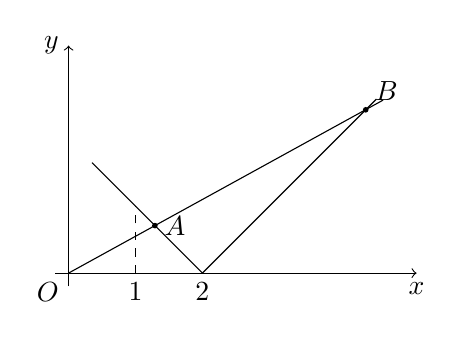
\begin{tikzpicture}[scale=0.85]
\draw[->] (-0.2,0) -- (5.2,0) node[below]{$x$};
\draw[->] (0,-0.2) -- (0,3.4) node[left]{$y$};
\node[below left] at (0,0) {$O$};
\draw (2,0) -- (0.35,1.65);
\draw (2,0) -- (4.6,2.6);
\draw (0,0) -- (4.7,2.585);
\draw[dashed] (1,0) -- (1,1);
\node[below] at (1,0) {$1$};
\node[below] at (2,0) {$2$};
\coordinate (A) at (1.29,0.71); \fill (A) circle (1.2pt); \node[right] at (A) {$A$};
\coordinate (B) at (4.44,2.44); \fill (B) circle (1.2pt); \node[above right] at (B) {$B$};
\end{tikzpicture}
\end{center}
\step{由 $0<k<1$，得 $x_A>1$，}
\step{所以关于 $x$ 的不等式 $k\lvert x\rvert-\lvert x-2\rvert>0$ 恰好有 $4$ 个整数解，是 $2,3,4,5$，}
\step{由 $\begin{cases}y=kx\\ y=x-2\end{cases}\Rightarrow x_B=\dfrac2{1-k}\in(5,6]$，故 $\dfrac35<k\leqslant\dfrac23$.}
\solend
\fi

\item 设集合 $S=\{1,2,3,\cdots,10\}$，$S$ 的子集 $A$ 满足 $A\cap\{1,2,3\}\neq\varnothing$，$A\cup\{4,5,6\}\neq S$，这样的子集 $A$ 的个数为\blankline[4.4em].

\ifanswer
\solbegin
\step{先求使 $A\cap\{1,2,3\}\neq\varnothing$ 成立的 $S$ 的子集 $A$ 的个数 $N_1$，}
\step{在 $\{1,2,3\}$ 中取出至少一个元素的方式有 $7$ 种，}
\step{而集合 $\{4,5,\cdots,10\}$ 的子集有 $2^7$ 个，因此 $N_1=7\times2^7=896$，}
% 注：下一行原卷印作“$A\cup\{4,5,6\}\neq S$”，按上下文应为“$=S$”，照录未改（见文件头“原卷笔误/存疑”①）。
\step{再扣除其中使 $A\cup\{4,5,6\}\neq S$ 的集合 $A$ 的个数 $N_2$，}
\step{这些取法中 $1$，$2$，$3$，$7$，$8$，$9$，$10$ 均被取出，}
\step{而集合 $\{4,5,6\}$ 的子集有 $2^3$ 个，因此 $N_2=2^3=8$，}
\step{从而满足条件的子集 $A$ 的个数为 $N_1-N_2=896-8=888$.}
\solend
\fi

\end{enumerate}

\bigsec{二、选择题}

\begin{enumerate}
\setcounter{enumi}{12}

\item 已知 $a>b$，下列不等式中一定成立是\mbox{（\quad）}

\keepwithprev
A. $a^2>b^2$\qquad B. $ac^2>bc^2$\qquad C. $\dfrac1a<\dfrac1b$\qquad D. $a+3>b-4$

\ifanswer
\solbegin
\step{对于 $A$，当 $a=-2$，$b=-4$ 时，不等式不成立，故 $A$ 错误；}
\step{对于 $B$，当 $c=0$ 时，不等式不成立，故 $B$ 错误；}
\step{对于 $C$，当 $a=2$，$b=-4$ 时，不等式不成立，故 $C$ 错误；}
\step{对于 $D$，因为 $a>b$，$3>-4$，必有 $a+3>b-4$ 成立，故 $D$ 正确.}
\solend
\fi

\item 已知集合 $M$ 满足 $\{2,3\}\subseteq M\subseteq\{1,2,3,4,5\}$，那么这样的集合 $M$ 的个数为\mbox{（\quad）}

\keepwithprev
A. $6$\qquad B. $7$\qquad C. $8$\qquad D. $9$

\ifanswer
\solbegin
\step{集合 $M$ 满足 $\{2,3\}\subseteq M\subseteq\{1,2,3,4,5\}$，所以 $2\in M$，$3\in M$，}
\step{故集合 $M$ 的个数为 $2^3=8$. 故选 $C$.}
\solend
\fi

\item 已知集合 $A=\{x\mid x=2k,k\in\Z\}$，$B=\{x\mid x=4m+6n,m,n\in\Z\}$，则\mbox{（\quad）}

\keepwithprev
A. $B\subset A$\qquad B. $A\subset B$\qquad C. $A=B$\qquad D. $B\neq A$

\ifanswer
\solbegin
\step{$B=\{x\mid x=4m+6n,m,n\in\Z\}$，$B$ 中的元素都是偶数，}
\step{所以 $B$ 的元素都是 $A$ 的元素，$B\subseteq A$；}
\step{$A=\{x\mid x=4(-k)+6k,k\in\Z\}$，则 $A$ 的元素都是 $B$ 的元素，$A\subseteq B$；}
\step{所以 $A=B$. 故选 $C$.}
\solend
\fi

\item 已知集合 $A=[1,a]\cup[a^3,a^4]$，集合 $B=\{x\mid x=x_1-x_2$，其中 $x_1,x_2\in A\}$. 若集合 $B$ 表示的区间为一个闭区间，则 $a$ 的取值范围为\mbox{（\quad）}

\keepwithprev
A. $a$ 取遍任意大于 $1$ 的实数\qquad B. $a\geqslant2$

C. $a\geqslant\dfrac{1+\sqrt5}2$\qquad D. $a\geqslant1+\sqrt2$

\ifanswer
\solbegin
\step{由题意得 $a^3>a>1$，则 $x_1-x_2$ 的最小值为 $1-a^4$，最大值为 $a^4-1$，}
\step{所以 $B=[1-a^4,a^4-1]$，}
\step{又因为 $a^4-a^3-(a-1)=a^3(a-1)-(a-1)=(a^3-1)(a-1)>0$，}
\step{所以 $a^4-a^3>a-1$，又集合 $B$ 表示的区间为一个闭区间，}
\step{则 $a^3-a\leqslant a^4-a^3$，化简得 $a^2-a-1\geqslant0$，又 $a>1$，解得 $a\geqslant\dfrac{1+\sqrt5}2$.}
\step{故选 $C$.}
\solend
\fi

\end{enumerate}

\bigsec{三、解答题}

\begin{enumerate}
\setcounter{enumi}{16}

\item 设全集 $U=\R$，集合 $A=\{x\mid\lvert x+3\rvert\leqslant4\}$，集合 $B=\{x\mid a-2\leqslant x\leqslant1+2a\}$，其中 $a\in\R$.

（1）若 $a=\dfrac12$，求 $A\cap B$；

（2）若 $A\cap B=\varnothing$，求 $a$ 的取值范围.

\ifanswer
\solbegin
\stepm{(1)}{由 $\lvert x+3\rvert\leqslant4$，得 $-4\leqslant x+3\leqslant4$，解得 $-7\leqslant x\leqslant1$，}
\step{所以 $A=\{x\mid-7\leqslant x\leqslant1\}$，}
\step{当 $a=\dfrac12$ 时，$a-2=\dfrac12-2=-\dfrac32$，$1+2a=1+2\times\dfrac12=2$，}
\step{$B=\left\{x\mid-\dfrac32\leqslant x\leqslant2\right\}$，$A\cap B=\left\{x\mid-\dfrac32\leqslant x\leqslant1\right\}$，即 $\left[-\dfrac32,1\right]$.}
\stepm{(2)}{若 $A\cap B=\varnothing$，分两种情况讨论，}
\step{①当 $B\neq\varnothing$ 时，$a-2\leqslant1+2a$，即 $a\geqslant-3$，}
\step{要满足 $A\cap B=\varnothing$，则 $1+2a<-7$ 或 $a-2>1$，}
\step{由 $1+2a<-7$，得 $a<-4$，与 $a\geqslant-3$ 无交集，无解，}
\step{由 $a-2>1$ 得 $a>3$，符合 $a\geqslant-3$，}
\step{②当 $B=\varnothing$ 时，有 $a-2>1+2a$，解得 $a<-3$，满足 $A\cap B=\varnothing$；}
\step{综上，$a$ 的取值范围是 $(-\infty,-3)\cup(3,+\infty)$.}
\solend
\fi

\ansspace

\item （1）已知 $a>b>0$，比较 $\dfrac{a+b}{a^2+b^2}$ 与 $\dfrac1{a-b}$ 的大小并说明理由；

（2）已知 $-2\leqslant x\leqslant-1$，$2\leqslant y\leqslant3$，求 $2x-y$ 的取值范围.

\ifanswer
\solbegin
\stepm{(1)}{$\dfrac{a+b}{a^2+b^2}-\dfrac1{a-b}=\dfrac{(a^2-b^2)-(a^2+b^2)}{(a^2+b^2)(a-b)}=\dfrac{-2b^2}{(a^2+b^2)(a-b)}$，}
\step{因为 $a>b>0$，所以 $a^2(a-b)-b^2(b-a)=(a^2+b^2)(a-b)>0$，}
\step{$\dfrac{-2b^2}{(a^2+b^2)(a-b)}<0$，即 $\dfrac{a+b}{a^2+b^2}-\dfrac1{a-b}<0$，所以 $\dfrac{a+b}{a^2+b^2}<\dfrac1{a-b}$；}
\stepm{(2)}{由 $-2\leqslant x\leqslant-1$，$2\leqslant y\leqslant3$，得 $-4\leqslant2x\leqslant-2$，$-3\leqslant-y\leqslant-2$，}
\step{得 $-7\leqslant2x-y\leqslant-4$，即 $2x-y$ 的取值范围为 $[-7,-4]$.}
\solend
\fi

\ansspace

\item 设 $x_1$、$x_2$ 是关于 $x$ 的方程 $x^2-2(m+2)x+m^2-1=0$ 的两个实数根.

（1）若 $\dfrac1{x_1}+\dfrac1{x_2}=-4$，求 $m$ 的值；

（2）若 $x_1$、$x_2$ 是两个不相等的正数，求实数 $m$ 的取值范围.

\ifanswer
\solbegin
\stepm{(1)}{因为 $x_1$、$x_2$ 是关于 $x$ 的方程的两个实数根，}
\step{所以 $\Delta=(-2(m+2))^2-4(m^2-1)=16m+20\geqslant0$，解得 $m\geqslant-\dfrac54$，}
\step{由韦达定理得 $x_1+x_2=2(m+2)$，$x_1x_2=m^2-1$，}
\step{所以 $\dfrac1{x_1}+\dfrac1{x_2}=\dfrac{x_2+x_1}{x_1x_2}=\dfrac{2(m+2)}{m^2-1}=-4$，即 $2m^2+m=0$，}
\step{解得 $m=0$ 或 $m=-\dfrac12$；}
\stepm{(2)}{由题意得 $\begin{cases}x_1+x_2>0\\ x_1x_2>0\\ \Delta>0\end{cases}$，即 $\begin{cases}2(m+2)>0\\ m^2-1>0\\ (-2(m+2))^2-4(m^2-1)>0\end{cases}$，}
\step{解得 $-\dfrac54<m<-1$ 或 $m>1$.}
\solend
\fi

\ansspace

\ifanswer\else\needvspace{10\baselineskip}\fi
\item 已知集合 $A=\{x\mid x\leqslant2\text{ 或 }x\geqslant a\}$.

（1）若 $B=\left\{x\mid(x-2)\left(x-\dfrac{12}{7-a}\right)<0\right\}$，$A\cap B=\varnothing$，$A\cup B=\R$，求实数 $a$ 的值；

（2）若 $a=3$ 且 $b<2$，$B=\{x\mid x^2-b(b+1)x+b^3<0\}$，$A\cap B\cap\Z$ 的子集个数为 $4$ 个，求实数 $b$ 的取值范围.

\ifanswer
\solbegin
\stepm{(1)}{当 $a\leqslant2$ 时，$A=\{x\mid x\leqslant2\text{ 或 }x\geqslant a\}=\R$，必有 $B=\varnothing$，}
\step{即不等式 $(x-2)\left(x-\dfrac{12}{7-a}\right)<0$ 无解，}
\step{必有 $\dfrac{12}{7-a}=2$，解得 $a=1$，符合题意，}
\step{当 $a>2$ 时，$A=(-\infty,2]\cup[a,+\infty)$，}
\step{若 $A\cap B=\varnothing$，$A\cup B=\R$，则 $B=(2,a)$，}
\step{即方程 $(x-2)\left(x-\dfrac{12}{7-a}\right)=0$ 的两个根是 $2$ 和 $a$，所以 $\dfrac{12}{7-a}=a$，}
\step{解得 $a=3$ 或 $a=4$，符合题意，}
\step{综上，实数 $a$ 的值为 $1$ 或 $3$ 或 $4$；}
\stepm{(2)}{由 $A\cap B\cap\Z$ 的子集个数为 $4$ 个，即 $A\cap B\cap\Z$ 中恰好有 $2$ 个整数元素，}
\step{由 $a=3$，则 $A=(-\infty,2]\cup[3,+\infty)$，}
\step{由 $x^2-b(b+1)x+b^3=(x-b^2)(x-b)<0$，又 $b<2$，}
\step{当 $1<b<2$ 时，$1<b^2<4$ 且 $b^2>b$，则 $B=(b,b^2)$，}
\step{则 $A\cap B=(b,2]\cup[3,b^2)$，}
\step{要使 $A\cap B\cap\Z$ 中恰好有 $2$ 个整数元素，即 $A\cap B\cap\Z=\{2,3\}$，}
\step{即 $\begin{cases}1<b<2\\ 3<b^2<4\end{cases}$，解得 $\sqrt3<b<2$，符合题意，}
\step{当 $b=1$ 或 $b=0$ 时，$B=\varnothing$，此时 $A\cap B\cap\Z=\varnothing$，不符合题意，舍去，}
\step{当 $0<b<1$ 时，$0<b^2<1$ 且 $b^2<b$，则 $B=(b^2,b)$，}
\step{此时 $A\cap B\cap\Z=\varnothing$，不符合题意，舍去，}
\step{当 $-1<b<0$ 时，$0<b^2<1$ 且 $b^2>b$，则 $B=(b,b^2)$，}
\step{此时 $A\cap B\cap\Z=\{0\}$，即 $A\cap B\cap\Z$ 中只有 $1$ 个元素，不符合题意，舍去，}
\step{当 $b\leqslant-1$ 时，$b^2\geqslant1$ 且 $b^2>b$，则 $B=(b,b^2)$，}
\step{此时 $A\cap B\cap\Z\supseteq\{-1,0,1\}$，即 $A\cap B\cap\Z$ 中至少有 $3$ 个元素，}
\step{不符合题意，舍去，}
\step{综上，实数 $b$ 的取值范围为 $(\sqrt3,2)$.}
\solend
\fi

\ansspace*[7]

\item 已知集合 $A=\{a_1,a_2,a_3,\cdots,a_n\}$ 中的元素均为正整数，其中 $n\in\N$ 且 $n\geqslant3$. 若对任意 $x,y\in A(x\neq y)$，都有 $\lvert x-y\rvert\geqslant\dfrac{xy}k$，则称集合 $A$ 具有性质 $M_k$.

（1）集合 $A=\{1,2,a\}$ 具有性质 $M_3$，求 $a$ 的最小值；

（2）若集合 $A$ 具有性质 $M_{24}$，且 $A$ 中最小元素和最大元素分别为 $a,b$，求证：$\dfrac1a-\dfrac1b\geqslant\dfrac{n-1}{24}$；

（3）已知集合 $A$ 具有性质 $M_{24}$，求 $A$ 中元素个数的最大值，并说明理由.

\ifanswer
\solbegin
\stepm{(1)}{由性质 $M_3$ 定义得 $\begin{cases}a-1\geqslant\dfrac a3\\ a-2\geqslant\dfrac{2a}3\end{cases}\Rightarrow\begin{cases}a\geqslant\dfrac32\\ a\geqslant6\end{cases}\Rightarrow a\geqslant6$，且 $a\subseteq\N^*$，}
% 注：上一行原卷印作“$a\subseteq\N^*$”，应为“$a\in\N^*$”，照录未改（见文件头“原卷笔误/存疑”②）。
\step{所以 $a$ 的最小值为 $6$.}
\stepm{(2)}{由题意得 $\lvert a_i-a_{i+1}\rvert\geqslant\dfrac{a_ia_{i+1}}{24}$，$(i=1,2,3,\cdots,n-1)$，且 $a_1<\cdots<a_n$，}
\step{所以 $a_{i+1}-a_i\geqslant\dfrac{a_ia_{i+1}}{24}\Rightarrow\dfrac1{a_i}-\dfrac1{a_{i+1}}\geqslant\dfrac1{24}$，$(i=1,2,3,\cdots,n-1)$，}
\step{所以 $\dfrac1{a_1}-\dfrac1{a_2}+\dfrac1{a_2}-\dfrac1{a_3}+\cdots+\dfrac1{a_{n-1}}-\dfrac1{a_n}=\dfrac1{a_1}-\dfrac1{a_n}\geqslant\dfrac{n-1}{24}$，得证.}
\stepm{(3)}{由 (2) 得 $\begin{cases}\dfrac1{a_1}\geqslant\dfrac{n-1}{24}\\ a_1\geqslant1\end{cases}\Rightarrow\dfrac{n-1}{24}<1\Rightarrow n<25$，}
\step{同 (2) 证明得 $\dfrac1{a_i}-\dfrac1{a_n}\geqslant\dfrac{n-i}{24}$ 且 $i=1,2,3,\cdots,n-1$，故 $\dfrac1{a_i}>\dfrac{n-i}{24}$，}
\step{又 $a_i\geqslant i$，所以 $\dfrac1i>\dfrac{n-i}{24}\Rightarrow i(n-i)<24$ 在 $i=1,2,3,\cdots,n-1$ 上恒成立，}
\step{当 $n\geqslant10$，取 $i=5$，则 $i(n-i)=5(n-5)>24$，故 $n<10$，}
\step{当 $n\leqslant9$，则 $i(n-i)\leqslant\dfrac{(i+n-i)^2}4=\dfrac{n^2}4<24\Rightarrow n<\sqrt{96}$，即 $n\leqslant9$.}
\step{综上，集合 $A$ 中元素个数的最大值为 $9$.}
\solend
\fi

\end{enumerate}

\end{document}
"
% 紧凑版：xelatex "\def\iscompact{1}% 高一79_南汇中学_10月月考.tex
%   —— 高一上数学“2026-2027 年南汇中学高一上 10 月月考”（讲评版）
% 试卷版：xelatex 高一79_南汇中学_10月月考.tex
% 答案版：xelatex "\def\isanswer{1}\input{高一79_南汇中学_10月月考.tex}"
% 紧凑版：xelatex "\def\iscompact{1}\input{高一79_南汇中学_10月月考.tex}"
%
% 原始材料：微信公众号“魔都数学加油站”文章，连载“27学年高一79”；
% 原文标题“27学年高一79——2026-2027年上海市南汇中学高一上10月月考”；
% 原文链接：https://mp.weixin.qq.com/s/bFvc7GVgPTaDGg_6JSSfGg。
% 页面标注发布时间 2026-10-24 21:00（上海）。
% 正文为 9 张 PNG 页（`原图/高一79_南汇中学_10月月考/01..09.png`），
% 尺寸混排（第 1、2、4、5、7、8 页为 4762×6735，第 3、6、9 页为 2560×3620），均按页序读取。
%
% 篇幅与题号：原卷自第 3 题起编号。填空题 3—12（10 题）、选择题 13—16（4 题）、
% 解答题 17—21（5 题），共 19 题。
%
% 讲评版：第 4 题只印【答案】，本稿只给 \ans{}；其余 18 题印【解析】。
% 选择题答案在解析末句“故选 D／C／C／C”。
%
% 副标题：原卷未印副标题。本稿按内容标作“集合与常用逻辑用语、不等式”。
%
% 原卷笔误/存疑（均照录未改，正文对应处另有 % 注）：
%   ① 第 12 题解析作“再扣除其中使 $A\cup\{4,5,6\}\neq S$ 的集合 $A$ 的个数 $N_2$”，
%      按上下文应为“$A\cup\{4,5,6\}=S$”，否则“这些取法中 $1,2,3,7,8,9,10$ 均被取出”
%      与 $N_2=2^3=8$ 都无法解释；原卷印作 $\neq$，照录未改。
%   ② 第 21 题 (1) 解析末作“且 $a\subseteq\N^*$”，$a$ 是集合的元素，应为 $a\in\N^*$；
%      原卷印作 $\subseteq$，照录未改。
%
% 与原卷的排版差异：
%   ① 原卷每题下直接印【答案】/【解析】，本稿按全稿惯例将答案与解析置于答案版；
%   ② 原卷未印副标题，本稿补出；填空横线统一排 \blankline[4.4em]；
%   ③ 原卷数集记号排斜体 $R$、$Z$、$N$，本稿按全稿惯例改用 $\R$、$\Z$、$\N$；
%   ④ 第 17—21 题的子问用行内“（1）（2）（3）”段，解析中的子问标号用 \stepm；
%   ⑤ 解答题按惯例加 \ansspace；选择题括号排 \mbox{（\quad）}；
%   ⑥ 第 11 题解析有一幅函数图象（$y=k\lvert x\rvert$ 与 $y=\lvert x-2\rvert$），
%      按原图形状用 TikZ 重排（仅答案版出）。
%
% 行数核对：逐题数 \step/\stepm 条数，合计 107 条（Q3：2；Q5：2；Q6：1；Q7：4；Q8：4；
% Q9：4；Q10：5；Q11：4；Q12：7；Q13：4；Q14：2；Q15：4；Q16：6；Q17：11；Q18：5；
% Q19：7；Q20：24；Q21：11）。原卷解析的换行按语意合并，未逐行强拆；第 4 题只印
% 【答案】，提 \ans{}，不计入 \step 账。
%
\documentclass[a4paper,11pt]{article}
\usepackage{common}

\begin{document}

\examtitlest[3]{2026--2027 年南汇中学高一上 10 月月考}{集合与常用逻辑用语、不等式}

\bigsec{一、填空题}

\begin{enumerate}
\setcounter{enumi}{2}

\item 不等式 $\dfrac{1-x}{x}>0$ 的解集为\blankline[4.4em].

\ifanswer
\solbegin
\step{原不等式化为 $x(x-1)<0$，转化为 $\begin{cases}x>0\\ x-1<0\end{cases}$ 或 $\begin{cases}x<0\\ x-1>0\end{cases}$，}
\step{解得 $0<x<1$，则不等式的解集为 $\{x\mid0<x<1\}$.}
\solend
\fi

\item 用反证法证明命题：“若 $x^2<1$，则 $-1<x<1$”时，应假设\blankline[4.4em].

\ifanswer
\ans{$x\geqslant1$ 或 $x\leqslant-1$}
\fi

\item 设 $k$ 为实数，关于 $x$ 的不等式 $kx^2+x+2<0$ 的解集为 $A$，若 $2\notin A$，则 $k$ 的取值范围是\blankline[4.4em].

\ifanswer
\solbegin
\step{因为关于 $x$ 的不等式 $kx^2+x+2<0$ 的解集为 $A$，且 $2\notin A$，}
\step{所以 $x=2$ 时，$k\times2^2+2+2\geqslant0$，解得 $k\geqslant-1$，则 $k$ 的取值范围为 $[-1,+\infty)$.}
\solend
\fi

\item 已知集合 $M=\{y\mid y=x^2-2x,x\in\R\}$，$N=\{x\mid y=\sqrt{4-x^2}\}$，则 $M\cup N=$\blankline[4.4em].

\ifanswer
\solbegin
\step{$M=[-1,+\infty)$，$N=[-2,2]$，则 $M\cup N=[-2,+\infty)$.}
\solend
\fi

\item 设集合 $A=\{-3,2\}$，集合 $B=\{x\mid mx+1=0\}$，且 $A\cup B=A$，则 $m$ 的值组成的集合是\blankline[4.4em].

\ifanswer
\solbegin
\step{由 $A\cup B=A$，得 $B\subseteq A$，}
\step{当 $m=0$ 时，$B=\varnothing$，满足题意，}
\step{当 $m\neq0$ 时，$B=\left\{-\dfrac1m\right\}$，所以 $-\dfrac1m=2$ 或 $-\dfrac1m=-3$，所以 $m=-\dfrac12$ 或 $m=\dfrac13$，}
\step{综上所述，$m$ 的值组成的集合是 $\left\{0,-\dfrac12,\dfrac13\right\}$.}
\solend
\fi

\item 若不等式 $\lvert x\rvert<a$ 的一个充分不必要条件为 $\dfrac{2x-1}{x-2}<1$，则实数 $a$ 的取值范围是\blankline[4.4em].

\ifanswer
\solbegin
\step{不等式 $\lvert x\rvert<a$，得 $-a<x<a$，}
\step{不等式 $\dfrac{2x-1}{x-2}<1$，即 $\dfrac{2x-1-(x-2)}{x-2}=\dfrac{x+1}{x-2}<0$，解得 $-1<x<2$，}
\step{又不等式 $\lvert x\rvert<a$ 的一个充分不必要条件为 $\dfrac{2x-1}{x-2}<1$，}
\step{得 $\begin{cases}a\geqslant2\\ -a\leqslant-1\end{cases}$，且两等号不同时成立，解得 $a\geqslant2$.}
\solend
\fi

\item 若对任意 $x\in\R$ 都有 $(m-1)x^2-(m-1)x-1<0$，则实数 $m$ 的取值范围是\blankline[4.4em].

\ifanswer
\solbegin
\step{当 $m-1\neq0$，即 $m\neq1$ 时，则有 $\begin{cases}m-1<0\\ (m-1)^2-4(m-1)\times(-1)<0\end{cases}$，}
\step{解得 $-3<m<1$；}
\step{当 $m-1=0$ 时，即当 $m=1$ 时，此时不等式为 $-1<0$ 恒成立，符合题意；}
\step{综上所述，实数 $m$ 的取值范围是 $(-3,1]$.}
\solend
\fi

\item 关于 $x$ 的方程 $\dfrac{x}{x-1}=\dfrac{k-x}{x^2-x}$ 的解集中只含有一个元素，则 $k$ 的可能取值构成的集合为\blankline[4.4em].

\ifanswer
\solbegin
\step{方程两边同时乘以 $x(x-1)$ 得 $x^2=k-x$，即 $x^2+x-k=0$，}
\step{①当其中一个解为增根时，方程也只有一个解，}
\step{(i) 若增根为 $0$ 时，$k=0$；(ii) 若增根为 $1$ 时，$k=2$；}
\step{②当 $\Delta=1+4k=0$，即 $k=-\dfrac14$ 时，方程 $x^2+x-k=0$ 只有一个解；}
\step{即 $k$ 的可能取值构成的集合为 $\left\{-\dfrac14,0,2\right\}$.}
\solend
\fi

\item 若关于 $x$ 的不等式 $k\lvert x\rvert>\lvert x-2\rvert$ 恰好有 $4$ 个整数解，则实数 $k$ 的取值范围是\blankline[4.4em].

\ifanswer
\solbegin
\step{由题意得 $0<k<1$，函数 $y=k\lvert x\rvert$ 与 $y=\lvert x-2\rvert$ 的图象如图：}
\begin{center}
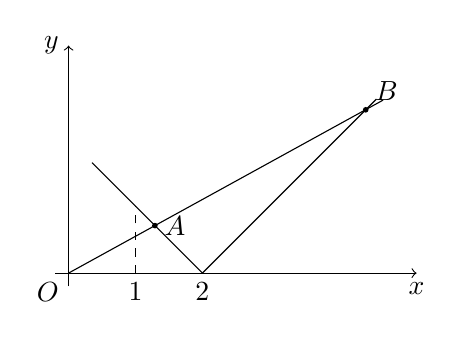
\begin{tikzpicture}[scale=0.85]
\draw[->] (-0.2,0) -- (5.2,0) node[below]{$x$};
\draw[->] (0,-0.2) -- (0,3.4) node[left]{$y$};
\node[below left] at (0,0) {$O$};
\draw (2,0) -- (0.35,1.65);
\draw (2,0) -- (4.6,2.6);
\draw (0,0) -- (4.7,2.585);
\draw[dashed] (1,0) -- (1,1);
\node[below] at (1,0) {$1$};
\node[below] at (2,0) {$2$};
\coordinate (A) at (1.29,0.71); \fill (A) circle (1.2pt); \node[right] at (A) {$A$};
\coordinate (B) at (4.44,2.44); \fill (B) circle (1.2pt); \node[above right] at (B) {$B$};
\end{tikzpicture}
\end{center}
\step{由 $0<k<1$，得 $x_A>1$，}
\step{所以关于 $x$ 的不等式 $k\lvert x\rvert-\lvert x-2\rvert>0$ 恰好有 $4$ 个整数解，是 $2,3,4,5$，}
\step{由 $\begin{cases}y=kx\\ y=x-2\end{cases}\Rightarrow x_B=\dfrac2{1-k}\in(5,6]$，故 $\dfrac35<k\leqslant\dfrac23$.}
\solend
\fi

\item 设集合 $S=\{1,2,3,\cdots,10\}$，$S$ 的子集 $A$ 满足 $A\cap\{1,2,3\}\neq\varnothing$，$A\cup\{4,5,6\}\neq S$，这样的子集 $A$ 的个数为\blankline[4.4em].

\ifanswer
\solbegin
\step{先求使 $A\cap\{1,2,3\}\neq\varnothing$ 成立的 $S$ 的子集 $A$ 的个数 $N_1$，}
\step{在 $\{1,2,3\}$ 中取出至少一个元素的方式有 $7$ 种，}
\step{而集合 $\{4,5,\cdots,10\}$ 的子集有 $2^7$ 个，因此 $N_1=7\times2^7=896$，}
% 注：下一行原卷印作“$A\cup\{4,5,6\}\neq S$”，按上下文应为“$=S$”，照录未改（见文件头“原卷笔误/存疑”①）。
\step{再扣除其中使 $A\cup\{4,5,6\}\neq S$ 的集合 $A$ 的个数 $N_2$，}
\step{这些取法中 $1$，$2$，$3$，$7$，$8$，$9$，$10$ 均被取出，}
\step{而集合 $\{4,5,6\}$ 的子集有 $2^3$ 个，因此 $N_2=2^3=8$，}
\step{从而满足条件的子集 $A$ 的个数为 $N_1-N_2=896-8=888$.}
\solend
\fi

\end{enumerate}

\bigsec{二、选择题}

\begin{enumerate}
\setcounter{enumi}{12}

\item 已知 $a>b$，下列不等式中一定成立是\mbox{（\quad）}

\keepwithprev
A. $a^2>b^2$\qquad B. $ac^2>bc^2$\qquad C. $\dfrac1a<\dfrac1b$\qquad D. $a+3>b-4$

\ifanswer
\solbegin
\step{对于 $A$，当 $a=-2$，$b=-4$ 时，不等式不成立，故 $A$ 错误；}
\step{对于 $B$，当 $c=0$ 时，不等式不成立，故 $B$ 错误；}
\step{对于 $C$，当 $a=2$，$b=-4$ 时，不等式不成立，故 $C$ 错误；}
\step{对于 $D$，因为 $a>b$，$3>-4$，必有 $a+3>b-4$ 成立，故 $D$ 正确.}
\solend
\fi

\item 已知集合 $M$ 满足 $\{2,3\}\subseteq M\subseteq\{1,2,3,4,5\}$，那么这样的集合 $M$ 的个数为\mbox{（\quad）}

\keepwithprev
A. $6$\qquad B. $7$\qquad C. $8$\qquad D. $9$

\ifanswer
\solbegin
\step{集合 $M$ 满足 $\{2,3\}\subseteq M\subseteq\{1,2,3,4,5\}$，所以 $2\in M$，$3\in M$，}
\step{故集合 $M$ 的个数为 $2^3=8$. 故选 $C$.}
\solend
\fi

\item 已知集合 $A=\{x\mid x=2k,k\in\Z\}$，$B=\{x\mid x=4m+6n,m,n\in\Z\}$，则\mbox{（\quad）}

\keepwithprev
A. $B\subset A$\qquad B. $A\subset B$\qquad C. $A=B$\qquad D. $B\neq A$

\ifanswer
\solbegin
\step{$B=\{x\mid x=4m+6n,m,n\in\Z\}$，$B$ 中的元素都是偶数，}
\step{所以 $B$ 的元素都是 $A$ 的元素，$B\subseteq A$；}
\step{$A=\{x\mid x=4(-k)+6k,k\in\Z\}$，则 $A$ 的元素都是 $B$ 的元素，$A\subseteq B$；}
\step{所以 $A=B$. 故选 $C$.}
\solend
\fi

\item 已知集合 $A=[1,a]\cup[a^3,a^4]$，集合 $B=\{x\mid x=x_1-x_2$，其中 $x_1,x_2\in A\}$. 若集合 $B$ 表示的区间为一个闭区间，则 $a$ 的取值范围为\mbox{（\quad）}

\keepwithprev
A. $a$ 取遍任意大于 $1$ 的实数\qquad B. $a\geqslant2$

C. $a\geqslant\dfrac{1+\sqrt5}2$\qquad D. $a\geqslant1+\sqrt2$

\ifanswer
\solbegin
\step{由题意得 $a^3>a>1$，则 $x_1-x_2$ 的最小值为 $1-a^4$，最大值为 $a^4-1$，}
\step{所以 $B=[1-a^4,a^4-1]$，}
\step{又因为 $a^4-a^3-(a-1)=a^3(a-1)-(a-1)=(a^3-1)(a-1)>0$，}
\step{所以 $a^4-a^3>a-1$，又集合 $B$ 表示的区间为一个闭区间，}
\step{则 $a^3-a\leqslant a^4-a^3$，化简得 $a^2-a-1\geqslant0$，又 $a>1$，解得 $a\geqslant\dfrac{1+\sqrt5}2$.}
\step{故选 $C$.}
\solend
\fi

\end{enumerate}

\bigsec{三、解答题}

\begin{enumerate}
\setcounter{enumi}{16}

\item 设全集 $U=\R$，集合 $A=\{x\mid\lvert x+3\rvert\leqslant4\}$，集合 $B=\{x\mid a-2\leqslant x\leqslant1+2a\}$，其中 $a\in\R$.

（1）若 $a=\dfrac12$，求 $A\cap B$；

（2）若 $A\cap B=\varnothing$，求 $a$ 的取值范围.

\ifanswer
\solbegin
\stepm{(1)}{由 $\lvert x+3\rvert\leqslant4$，得 $-4\leqslant x+3\leqslant4$，解得 $-7\leqslant x\leqslant1$，}
\step{所以 $A=\{x\mid-7\leqslant x\leqslant1\}$，}
\step{当 $a=\dfrac12$ 时，$a-2=\dfrac12-2=-\dfrac32$，$1+2a=1+2\times\dfrac12=2$，}
\step{$B=\left\{x\mid-\dfrac32\leqslant x\leqslant2\right\}$，$A\cap B=\left\{x\mid-\dfrac32\leqslant x\leqslant1\right\}$，即 $\left[-\dfrac32,1\right]$.}
\stepm{(2)}{若 $A\cap B=\varnothing$，分两种情况讨论，}
\step{①当 $B\neq\varnothing$ 时，$a-2\leqslant1+2a$，即 $a\geqslant-3$，}
\step{要满足 $A\cap B=\varnothing$，则 $1+2a<-7$ 或 $a-2>1$，}
\step{由 $1+2a<-7$，得 $a<-4$，与 $a\geqslant-3$ 无交集，无解，}
\step{由 $a-2>1$ 得 $a>3$，符合 $a\geqslant-3$，}
\step{②当 $B=\varnothing$ 时，有 $a-2>1+2a$，解得 $a<-3$，满足 $A\cap B=\varnothing$；}
\step{综上，$a$ 的取值范围是 $(-\infty,-3)\cup(3,+\infty)$.}
\solend
\fi

\ansspace

\item （1）已知 $a>b>0$，比较 $\dfrac{a+b}{a^2+b^2}$ 与 $\dfrac1{a-b}$ 的大小并说明理由；

（2）已知 $-2\leqslant x\leqslant-1$，$2\leqslant y\leqslant3$，求 $2x-y$ 的取值范围.

\ifanswer
\solbegin
\stepm{(1)}{$\dfrac{a+b}{a^2+b^2}-\dfrac1{a-b}=\dfrac{(a^2-b^2)-(a^2+b^2)}{(a^2+b^2)(a-b)}=\dfrac{-2b^2}{(a^2+b^2)(a-b)}$，}
\step{因为 $a>b>0$，所以 $a^2(a-b)-b^2(b-a)=(a^2+b^2)(a-b)>0$，}
\step{$\dfrac{-2b^2}{(a^2+b^2)(a-b)}<0$，即 $\dfrac{a+b}{a^2+b^2}-\dfrac1{a-b}<0$，所以 $\dfrac{a+b}{a^2+b^2}<\dfrac1{a-b}$；}
\stepm{(2)}{由 $-2\leqslant x\leqslant-1$，$2\leqslant y\leqslant3$，得 $-4\leqslant2x\leqslant-2$，$-3\leqslant-y\leqslant-2$，}
\step{得 $-7\leqslant2x-y\leqslant-4$，即 $2x-y$ 的取值范围为 $[-7,-4]$.}
\solend
\fi

\ansspace

\item 设 $x_1$、$x_2$ 是关于 $x$ 的方程 $x^2-2(m+2)x+m^2-1=0$ 的两个实数根.

（1）若 $\dfrac1{x_1}+\dfrac1{x_2}=-4$，求 $m$ 的值；

（2）若 $x_1$、$x_2$ 是两个不相等的正数，求实数 $m$ 的取值范围.

\ifanswer
\solbegin
\stepm{(1)}{因为 $x_1$、$x_2$ 是关于 $x$ 的方程的两个实数根，}
\step{所以 $\Delta=(-2(m+2))^2-4(m^2-1)=16m+20\geqslant0$，解得 $m\geqslant-\dfrac54$，}
\step{由韦达定理得 $x_1+x_2=2(m+2)$，$x_1x_2=m^2-1$，}
\step{所以 $\dfrac1{x_1}+\dfrac1{x_2}=\dfrac{x_2+x_1}{x_1x_2}=\dfrac{2(m+2)}{m^2-1}=-4$，即 $2m^2+m=0$，}
\step{解得 $m=0$ 或 $m=-\dfrac12$；}
\stepm{(2)}{由题意得 $\begin{cases}x_1+x_2>0\\ x_1x_2>0\\ \Delta>0\end{cases}$，即 $\begin{cases}2(m+2)>0\\ m^2-1>0\\ (-2(m+2))^2-4(m^2-1)>0\end{cases}$，}
\step{解得 $-\dfrac54<m<-1$ 或 $m>1$.}
\solend
\fi

\ansspace

\ifanswer\else\needvspace{10\baselineskip}\fi
\item 已知集合 $A=\{x\mid x\leqslant2\text{ 或 }x\geqslant a\}$.

（1）若 $B=\left\{x\mid(x-2)\left(x-\dfrac{12}{7-a}\right)<0\right\}$，$A\cap B=\varnothing$，$A\cup B=\R$，求实数 $a$ 的值；

（2）若 $a=3$ 且 $b<2$，$B=\{x\mid x^2-b(b+1)x+b^3<0\}$，$A\cap B\cap\Z$ 的子集个数为 $4$ 个，求实数 $b$ 的取值范围.

\ifanswer
\solbegin
\stepm{(1)}{当 $a\leqslant2$ 时，$A=\{x\mid x\leqslant2\text{ 或 }x\geqslant a\}=\R$，必有 $B=\varnothing$，}
\step{即不等式 $(x-2)\left(x-\dfrac{12}{7-a}\right)<0$ 无解，}
\step{必有 $\dfrac{12}{7-a}=2$，解得 $a=1$，符合题意，}
\step{当 $a>2$ 时，$A=(-\infty,2]\cup[a,+\infty)$，}
\step{若 $A\cap B=\varnothing$，$A\cup B=\R$，则 $B=(2,a)$，}
\step{即方程 $(x-2)\left(x-\dfrac{12}{7-a}\right)=0$ 的两个根是 $2$ 和 $a$，所以 $\dfrac{12}{7-a}=a$，}
\step{解得 $a=3$ 或 $a=4$，符合题意，}
\step{综上，实数 $a$ 的值为 $1$ 或 $3$ 或 $4$；}
\stepm{(2)}{由 $A\cap B\cap\Z$ 的子集个数为 $4$ 个，即 $A\cap B\cap\Z$ 中恰好有 $2$ 个整数元素，}
\step{由 $a=3$，则 $A=(-\infty,2]\cup[3,+\infty)$，}
\step{由 $x^2-b(b+1)x+b^3=(x-b^2)(x-b)<0$，又 $b<2$，}
\step{当 $1<b<2$ 时，$1<b^2<4$ 且 $b^2>b$，则 $B=(b,b^2)$，}
\step{则 $A\cap B=(b,2]\cup[3,b^2)$，}
\step{要使 $A\cap B\cap\Z$ 中恰好有 $2$ 个整数元素，即 $A\cap B\cap\Z=\{2,3\}$，}
\step{即 $\begin{cases}1<b<2\\ 3<b^2<4\end{cases}$，解得 $\sqrt3<b<2$，符合题意，}
\step{当 $b=1$ 或 $b=0$ 时，$B=\varnothing$，此时 $A\cap B\cap\Z=\varnothing$，不符合题意，舍去，}
\step{当 $0<b<1$ 时，$0<b^2<1$ 且 $b^2<b$，则 $B=(b^2,b)$，}
\step{此时 $A\cap B\cap\Z=\varnothing$，不符合题意，舍去，}
\step{当 $-1<b<0$ 时，$0<b^2<1$ 且 $b^2>b$，则 $B=(b,b^2)$，}
\step{此时 $A\cap B\cap\Z=\{0\}$，即 $A\cap B\cap\Z$ 中只有 $1$ 个元素，不符合题意，舍去，}
\step{当 $b\leqslant-1$ 时，$b^2\geqslant1$ 且 $b^2>b$，则 $B=(b,b^2)$，}
\step{此时 $A\cap B\cap\Z\supseteq\{-1,0,1\}$，即 $A\cap B\cap\Z$ 中至少有 $3$ 个元素，}
\step{不符合题意，舍去，}
\step{综上，实数 $b$ 的取值范围为 $(\sqrt3,2)$.}
\solend
\fi

\ansspace*[7]

\item 已知集合 $A=\{a_1,a_2,a_3,\cdots,a_n\}$ 中的元素均为正整数，其中 $n\in\N$ 且 $n\geqslant3$. 若对任意 $x,y\in A(x\neq y)$，都有 $\lvert x-y\rvert\geqslant\dfrac{xy}k$，则称集合 $A$ 具有性质 $M_k$.

（1）集合 $A=\{1,2,a\}$ 具有性质 $M_3$，求 $a$ 的最小值；

（2）若集合 $A$ 具有性质 $M_{24}$，且 $A$ 中最小元素和最大元素分别为 $a,b$，求证：$\dfrac1a-\dfrac1b\geqslant\dfrac{n-1}{24}$；

（3）已知集合 $A$ 具有性质 $M_{24}$，求 $A$ 中元素个数的最大值，并说明理由.

\ifanswer
\solbegin
\stepm{(1)}{由性质 $M_3$ 定义得 $\begin{cases}a-1\geqslant\dfrac a3\\ a-2\geqslant\dfrac{2a}3\end{cases}\Rightarrow\begin{cases}a\geqslant\dfrac32\\ a\geqslant6\end{cases}\Rightarrow a\geqslant6$，且 $a\subseteq\N^*$，}
% 注：上一行原卷印作“$a\subseteq\N^*$”，应为“$a\in\N^*$”，照录未改（见文件头“原卷笔误/存疑”②）。
\step{所以 $a$ 的最小值为 $6$.}
\stepm{(2)}{由题意得 $\lvert a_i-a_{i+1}\rvert\geqslant\dfrac{a_ia_{i+1}}{24}$，$(i=1,2,3,\cdots,n-1)$，且 $a_1<\cdots<a_n$，}
\step{所以 $a_{i+1}-a_i\geqslant\dfrac{a_ia_{i+1}}{24}\Rightarrow\dfrac1{a_i}-\dfrac1{a_{i+1}}\geqslant\dfrac1{24}$，$(i=1,2,3,\cdots,n-1)$，}
\step{所以 $\dfrac1{a_1}-\dfrac1{a_2}+\dfrac1{a_2}-\dfrac1{a_3}+\cdots+\dfrac1{a_{n-1}}-\dfrac1{a_n}=\dfrac1{a_1}-\dfrac1{a_n}\geqslant\dfrac{n-1}{24}$，得证.}
\stepm{(3)}{由 (2) 得 $\begin{cases}\dfrac1{a_1}\geqslant\dfrac{n-1}{24}\\ a_1\geqslant1\end{cases}\Rightarrow\dfrac{n-1}{24}<1\Rightarrow n<25$，}
\step{同 (2) 证明得 $\dfrac1{a_i}-\dfrac1{a_n}\geqslant\dfrac{n-i}{24}$ 且 $i=1,2,3,\cdots,n-1$，故 $\dfrac1{a_i}>\dfrac{n-i}{24}$，}
\step{又 $a_i\geqslant i$，所以 $\dfrac1i>\dfrac{n-i}{24}\Rightarrow i(n-i)<24$ 在 $i=1,2,3,\cdots,n-1$ 上恒成立，}
\step{当 $n\geqslant10$，取 $i=5$，则 $i(n-i)=5(n-5)>24$，故 $n<10$，}
\step{当 $n\leqslant9$，则 $i(n-i)\leqslant\dfrac{(i+n-i)^2}4=\dfrac{n^2}4<24\Rightarrow n<\sqrt{96}$，即 $n\leqslant9$.}
\step{综上，集合 $A$ 中元素个数的最大值为 $9$.}
\solend
\fi

\end{enumerate}

\end{document}
"
%
% 原始材料：微信公众号“魔都数学加油站”文章，连载“27学年高一79”；
% 原文标题“27学年高一79——2026-2027年上海市南汇中学高一上10月月考”；
% 原文链接：https://mp.weixin.qq.com/s/bFvc7GVgPTaDGg_6JSSfGg。
% 页面标注发布时间 2026-10-24 21:00（上海）。
% 正文为 9 张 PNG 页（`原图/高一79_南汇中学_10月月考/01..09.png`），
% 尺寸混排（第 1、2、4、5、7、8 页为 4762×6735，第 3、6、9 页为 2560×3620），均按页序读取。
%
% 篇幅与题号：原卷自第 3 题起编号。填空题 3—12（10 题）、选择题 13—16（4 题）、
% 解答题 17—21（5 题），共 19 题。
%
% 讲评版：第 4 题只印【答案】，本稿只给 \ans{}；其余 18 题印【解析】。
% 选择题答案在解析末句“故选 D／C／C／C”。
%
% 副标题：原卷未印副标题。本稿按内容标作“集合与常用逻辑用语、不等式”。
%
% 原卷笔误/存疑（均照录未改，正文对应处另有 % 注）：
%   ① 第 12 题解析作“再扣除其中使 $A\cup\{4,5,6\}\neq S$ 的集合 $A$ 的个数 $N_2$”，
%      按上下文应为“$A\cup\{4,5,6\}=S$”，否则“这些取法中 $1,2,3,7,8,9,10$ 均被取出”
%      与 $N_2=2^3=8$ 都无法解释；原卷印作 $\neq$，照录未改。
%   ② 第 21 题 (1) 解析末作“且 $a\subseteq\N^*$”，$a$ 是集合的元素，应为 $a\in\N^*$；
%      原卷印作 $\subseteq$，照录未改。
%
% 与原卷的排版差异：
%   ① 原卷每题下直接印【答案】/【解析】，本稿按全稿惯例将答案与解析置于答案版；
%   ② 原卷未印副标题，本稿补出；填空横线统一排 \blankline[4.4em]；
%   ③ 原卷数集记号排斜体 $R$、$Z$、$N$，本稿按全稿惯例改用 $\R$、$\Z$、$\N$；
%   ④ 第 17—21 题的子问用行内“（1）（2）（3）”段，解析中的子问标号用 \stepm；
%   ⑤ 解答题按惯例加 \ansspace；选择题括号排 \mbox{（\quad）}；
%   ⑥ 第 11 题解析有一幅函数图象（$y=k\lvert x\rvert$ 与 $y=\lvert x-2\rvert$），
%      按原图形状用 TikZ 重排（仅答案版出）。
%
% 行数核对：逐题数 \step/\stepm 条数，合计 107 条（Q3：2；Q5：2；Q6：1；Q7：4；Q8：4；
% Q9：4；Q10：5；Q11：4；Q12：7；Q13：4；Q14：2；Q15：4；Q16：6；Q17：11；Q18：5；
% Q19：7；Q20：24；Q21：11）。原卷解析的换行按语意合并，未逐行强拆；第 4 题只印
% 【答案】，提 \ans{}，不计入 \step 账。
%
\documentclass[a4paper,11pt]{article}
\usepackage{common}

\begin{document}

\examtitlest[3]{2026--2027 年南汇中学高一上 10 月月考}{集合与常用逻辑用语、不等式}

\bigsec{一、填空题}

\begin{enumerate}
\setcounter{enumi}{2}

\item 不等式 $\dfrac{1-x}{x}>0$ 的解集为\blankline[4.4em].

\ifanswer
\solbegin
\step{原不等式化为 $x(x-1)<0$，转化为 $\begin{cases}x>0\\ x-1<0\end{cases}$ 或 $\begin{cases}x<0\\ x-1>0\end{cases}$，}
\step{解得 $0<x<1$，则不等式的解集为 $\{x\mid0<x<1\}$.}
\solend
\fi

\item 用反证法证明命题：“若 $x^2<1$，则 $-1<x<1$”时，应假设\blankline[4.4em].

\ifanswer
\ans{$x\geqslant1$ 或 $x\leqslant-1$}
\fi

\item 设 $k$ 为实数，关于 $x$ 的不等式 $kx^2+x+2<0$ 的解集为 $A$，若 $2\notin A$，则 $k$ 的取值范围是\blankline[4.4em].

\ifanswer
\solbegin
\step{因为关于 $x$ 的不等式 $kx^2+x+2<0$ 的解集为 $A$，且 $2\notin A$，}
\step{所以 $x=2$ 时，$k\times2^2+2+2\geqslant0$，解得 $k\geqslant-1$，则 $k$ 的取值范围为 $[-1,+\infty)$.}
\solend
\fi

\item 已知集合 $M=\{y\mid y=x^2-2x,x\in\R\}$，$N=\{x\mid y=\sqrt{4-x^2}\}$，则 $M\cup N=$\blankline[4.4em].

\ifanswer
\solbegin
\step{$M=[-1,+\infty)$，$N=[-2,2]$，则 $M\cup N=[-2,+\infty)$.}
\solend
\fi

\item 设集合 $A=\{-3,2\}$，集合 $B=\{x\mid mx+1=0\}$，且 $A\cup B=A$，则 $m$ 的值组成的集合是\blankline[4.4em].

\ifanswer
\solbegin
\step{由 $A\cup B=A$，得 $B\subseteq A$，}
\step{当 $m=0$ 时，$B=\varnothing$，满足题意，}
\step{当 $m\neq0$ 时，$B=\left\{-\dfrac1m\right\}$，所以 $-\dfrac1m=2$ 或 $-\dfrac1m=-3$，所以 $m=-\dfrac12$ 或 $m=\dfrac13$，}
\step{综上所述，$m$ 的值组成的集合是 $\left\{0,-\dfrac12,\dfrac13\right\}$.}
\solend
\fi

\item 若不等式 $\lvert x\rvert<a$ 的一个充分不必要条件为 $\dfrac{2x-1}{x-2}<1$，则实数 $a$ 的取值范围是\blankline[4.4em].

\ifanswer
\solbegin
\step{不等式 $\lvert x\rvert<a$，得 $-a<x<a$，}
\step{不等式 $\dfrac{2x-1}{x-2}<1$，即 $\dfrac{2x-1-(x-2)}{x-2}=\dfrac{x+1}{x-2}<0$，解得 $-1<x<2$，}
\step{又不等式 $\lvert x\rvert<a$ 的一个充分不必要条件为 $\dfrac{2x-1}{x-2}<1$，}
\step{得 $\begin{cases}a\geqslant2\\ -a\leqslant-1\end{cases}$，且两等号不同时成立，解得 $a\geqslant2$.}
\solend
\fi

\item 若对任意 $x\in\R$ 都有 $(m-1)x^2-(m-1)x-1<0$，则实数 $m$ 的取值范围是\blankline[4.4em].

\ifanswer
\solbegin
\step{当 $m-1\neq0$，即 $m\neq1$ 时，则有 $\begin{cases}m-1<0\\ (m-1)^2-4(m-1)\times(-1)<0\end{cases}$，}
\step{解得 $-3<m<1$；}
\step{当 $m-1=0$ 时，即当 $m=1$ 时，此时不等式为 $-1<0$ 恒成立，符合题意；}
\step{综上所述，实数 $m$ 的取值范围是 $(-3,1]$.}
\solend
\fi

\item 关于 $x$ 的方程 $\dfrac{x}{x-1}=\dfrac{k-x}{x^2-x}$ 的解集中只含有一个元素，则 $k$ 的可能取值构成的集合为\blankline[4.4em].

\ifanswer
\solbegin
\step{方程两边同时乘以 $x(x-1)$ 得 $x^2=k-x$，即 $x^2+x-k=0$，}
\step{①当其中一个解为增根时，方程也只有一个解，}
\step{(i) 若增根为 $0$ 时，$k=0$；(ii) 若增根为 $1$ 时，$k=2$；}
\step{②当 $\Delta=1+4k=0$，即 $k=-\dfrac14$ 时，方程 $x^2+x-k=0$ 只有一个解；}
\step{即 $k$ 的可能取值构成的集合为 $\left\{-\dfrac14,0,2\right\}$.}
\solend
\fi

\item 若关于 $x$ 的不等式 $k\lvert x\rvert>\lvert x-2\rvert$ 恰好有 $4$ 个整数解，则实数 $k$ 的取值范围是\blankline[4.4em].

\ifanswer
\solbegin
\step{由题意得 $0<k<1$，函数 $y=k\lvert x\rvert$ 与 $y=\lvert x-2\rvert$ 的图象如图：}
\begin{center}
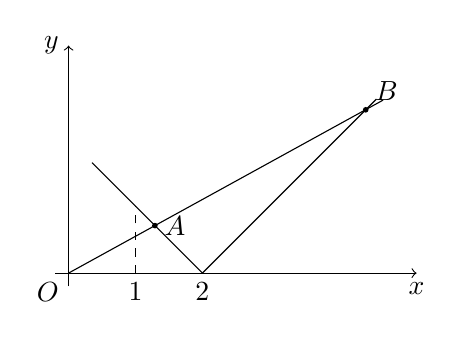
\begin{tikzpicture}[scale=0.85]
\draw[->] (-0.2,0) -- (5.2,0) node[below]{$x$};
\draw[->] (0,-0.2) -- (0,3.4) node[left]{$y$};
\node[below left] at (0,0) {$O$};
\draw (2,0) -- (0.35,1.65);
\draw (2,0) -- (4.6,2.6);
\draw (0,0) -- (4.7,2.585);
\draw[dashed] (1,0) -- (1,1);
\node[below] at (1,0) {$1$};
\node[below] at (2,0) {$2$};
\coordinate (A) at (1.29,0.71); \fill (A) circle (1.2pt); \node[right] at (A) {$A$};
\coordinate (B) at (4.44,2.44); \fill (B) circle (1.2pt); \node[above right] at (B) {$B$};
\end{tikzpicture}
\end{center}
\step{由 $0<k<1$，得 $x_A>1$，}
\step{所以关于 $x$ 的不等式 $k\lvert x\rvert-\lvert x-2\rvert>0$ 恰好有 $4$ 个整数解，是 $2,3,4,5$，}
\step{由 $\begin{cases}y=kx\\ y=x-2\end{cases}\Rightarrow x_B=\dfrac2{1-k}\in(5,6]$，故 $\dfrac35<k\leqslant\dfrac23$.}
\solend
\fi

\item 设集合 $S=\{1,2,3,\cdots,10\}$，$S$ 的子集 $A$ 满足 $A\cap\{1,2,3\}\neq\varnothing$，$A\cup\{4,5,6\}\neq S$，这样的子集 $A$ 的个数为\blankline[4.4em].

\ifanswer
\solbegin
\step{先求使 $A\cap\{1,2,3\}\neq\varnothing$ 成立的 $S$ 的子集 $A$ 的个数 $N_1$，}
\step{在 $\{1,2,3\}$ 中取出至少一个元素的方式有 $7$ 种，}
\step{而集合 $\{4,5,\cdots,10\}$ 的子集有 $2^7$ 个，因此 $N_1=7\times2^7=896$，}
% 注：下一行原卷印作“$A\cup\{4,5,6\}\neq S$”，按上下文应为“$=S$”，照录未改（见文件头“原卷笔误/存疑”①）。
\step{再扣除其中使 $A\cup\{4,5,6\}\neq S$ 的集合 $A$ 的个数 $N_2$，}
\step{这些取法中 $1$，$2$，$3$，$7$，$8$，$9$，$10$ 均被取出，}
\step{而集合 $\{4,5,6\}$ 的子集有 $2^3$ 个，因此 $N_2=2^3=8$，}
\step{从而满足条件的子集 $A$ 的个数为 $N_1-N_2=896-8=888$.}
\solend
\fi

\end{enumerate}

\bigsec{二、选择题}

\begin{enumerate}
\setcounter{enumi}{12}

\item 已知 $a>b$，下列不等式中一定成立是\mbox{（\quad）}

\keepwithprev
A. $a^2>b^2$\qquad B. $ac^2>bc^2$\qquad C. $\dfrac1a<\dfrac1b$\qquad D. $a+3>b-4$

\ifanswer
\solbegin
\step{对于 $A$，当 $a=-2$，$b=-4$ 时，不等式不成立，故 $A$ 错误；}
\step{对于 $B$，当 $c=0$ 时，不等式不成立，故 $B$ 错误；}
\step{对于 $C$，当 $a=2$，$b=-4$ 时，不等式不成立，故 $C$ 错误；}
\step{对于 $D$，因为 $a>b$，$3>-4$，必有 $a+3>b-4$ 成立，故 $D$ 正确.}
\solend
\fi

\item 已知集合 $M$ 满足 $\{2,3\}\subseteq M\subseteq\{1,2,3,4,5\}$，那么这样的集合 $M$ 的个数为\mbox{（\quad）}

\keepwithprev
A. $6$\qquad B. $7$\qquad C. $8$\qquad D. $9$

\ifanswer
\solbegin
\step{集合 $M$ 满足 $\{2,3\}\subseteq M\subseteq\{1,2,3,4,5\}$，所以 $2\in M$，$3\in M$，}
\step{故集合 $M$ 的个数为 $2^3=8$. 故选 $C$.}
\solend
\fi

\item 已知集合 $A=\{x\mid x=2k,k\in\Z\}$，$B=\{x\mid x=4m+6n,m,n\in\Z\}$，则\mbox{（\quad）}

\keepwithprev
A. $B\subset A$\qquad B. $A\subset B$\qquad C. $A=B$\qquad D. $B\neq A$

\ifanswer
\solbegin
\step{$B=\{x\mid x=4m+6n,m,n\in\Z\}$，$B$ 中的元素都是偶数，}
\step{所以 $B$ 的元素都是 $A$ 的元素，$B\subseteq A$；}
\step{$A=\{x\mid x=4(-k)+6k,k\in\Z\}$，则 $A$ 的元素都是 $B$ 的元素，$A\subseteq B$；}
\step{所以 $A=B$. 故选 $C$.}
\solend
\fi

\item 已知集合 $A=[1,a]\cup[a^3,a^4]$，集合 $B=\{x\mid x=x_1-x_2$，其中 $x_1,x_2\in A\}$. 若集合 $B$ 表示的区间为一个闭区间，则 $a$ 的取值范围为\mbox{（\quad）}

\keepwithprev
A. $a$ 取遍任意大于 $1$ 的实数\qquad B. $a\geqslant2$

C. $a\geqslant\dfrac{1+\sqrt5}2$\qquad D. $a\geqslant1+\sqrt2$

\ifanswer
\solbegin
\step{由题意得 $a^3>a>1$，则 $x_1-x_2$ 的最小值为 $1-a^4$，最大值为 $a^4-1$，}
\step{所以 $B=[1-a^4,a^4-1]$，}
\step{又因为 $a^4-a^3-(a-1)=a^3(a-1)-(a-1)=(a^3-1)(a-1)>0$，}
\step{所以 $a^4-a^3>a-1$，又集合 $B$ 表示的区间为一个闭区间，}
\step{则 $a^3-a\leqslant a^4-a^3$，化简得 $a^2-a-1\geqslant0$，又 $a>1$，解得 $a\geqslant\dfrac{1+\sqrt5}2$.}
\step{故选 $C$.}
\solend
\fi

\end{enumerate}

\bigsec{三、解答题}

\begin{enumerate}
\setcounter{enumi}{16}

\item 设全集 $U=\R$，集合 $A=\{x\mid\lvert x+3\rvert\leqslant4\}$，集合 $B=\{x\mid a-2\leqslant x\leqslant1+2a\}$，其中 $a\in\R$.

（1）若 $a=\dfrac12$，求 $A\cap B$；

（2）若 $A\cap B=\varnothing$，求 $a$ 的取值范围.

\ifanswer
\solbegin
\stepm{(1)}{由 $\lvert x+3\rvert\leqslant4$，得 $-4\leqslant x+3\leqslant4$，解得 $-7\leqslant x\leqslant1$，}
\step{所以 $A=\{x\mid-7\leqslant x\leqslant1\}$，}
\step{当 $a=\dfrac12$ 时，$a-2=\dfrac12-2=-\dfrac32$，$1+2a=1+2\times\dfrac12=2$，}
\step{$B=\left\{x\mid-\dfrac32\leqslant x\leqslant2\right\}$，$A\cap B=\left\{x\mid-\dfrac32\leqslant x\leqslant1\right\}$，即 $\left[-\dfrac32,1\right]$.}
\stepm{(2)}{若 $A\cap B=\varnothing$，分两种情况讨论，}
\step{①当 $B\neq\varnothing$ 时，$a-2\leqslant1+2a$，即 $a\geqslant-3$，}
\step{要满足 $A\cap B=\varnothing$，则 $1+2a<-7$ 或 $a-2>1$，}
\step{由 $1+2a<-7$，得 $a<-4$，与 $a\geqslant-3$ 无交集，无解，}
\step{由 $a-2>1$ 得 $a>3$，符合 $a\geqslant-3$，}
\step{②当 $B=\varnothing$ 时，有 $a-2>1+2a$，解得 $a<-3$，满足 $A\cap B=\varnothing$；}
\step{综上，$a$ 的取值范围是 $(-\infty,-3)\cup(3,+\infty)$.}
\solend
\fi

\ansspace

\item （1）已知 $a>b>0$，比较 $\dfrac{a+b}{a^2+b^2}$ 与 $\dfrac1{a-b}$ 的大小并说明理由；

（2）已知 $-2\leqslant x\leqslant-1$，$2\leqslant y\leqslant3$，求 $2x-y$ 的取值范围.

\ifanswer
\solbegin
\stepm{(1)}{$\dfrac{a+b}{a^2+b^2}-\dfrac1{a-b}=\dfrac{(a^2-b^2)-(a^2+b^2)}{(a^2+b^2)(a-b)}=\dfrac{-2b^2}{(a^2+b^2)(a-b)}$，}
\step{因为 $a>b>0$，所以 $a^2(a-b)-b^2(b-a)=(a^2+b^2)(a-b)>0$，}
\step{$\dfrac{-2b^2}{(a^2+b^2)(a-b)}<0$，即 $\dfrac{a+b}{a^2+b^2}-\dfrac1{a-b}<0$，所以 $\dfrac{a+b}{a^2+b^2}<\dfrac1{a-b}$；}
\stepm{(2)}{由 $-2\leqslant x\leqslant-1$，$2\leqslant y\leqslant3$，得 $-4\leqslant2x\leqslant-2$，$-3\leqslant-y\leqslant-2$，}
\step{得 $-7\leqslant2x-y\leqslant-4$，即 $2x-y$ 的取值范围为 $[-7,-4]$.}
\solend
\fi

\ansspace

\item 设 $x_1$、$x_2$ 是关于 $x$ 的方程 $x^2-2(m+2)x+m^2-1=0$ 的两个实数根.

（1）若 $\dfrac1{x_1}+\dfrac1{x_2}=-4$，求 $m$ 的值；

（2）若 $x_1$、$x_2$ 是两个不相等的正数，求实数 $m$ 的取值范围.

\ifanswer
\solbegin
\stepm{(1)}{因为 $x_1$、$x_2$ 是关于 $x$ 的方程的两个实数根，}
\step{所以 $\Delta=(-2(m+2))^2-4(m^2-1)=16m+20\geqslant0$，解得 $m\geqslant-\dfrac54$，}
\step{由韦达定理得 $x_1+x_2=2(m+2)$，$x_1x_2=m^2-1$，}
\step{所以 $\dfrac1{x_1}+\dfrac1{x_2}=\dfrac{x_2+x_1}{x_1x_2}=\dfrac{2(m+2)}{m^2-1}=-4$，即 $2m^2+m=0$，}
\step{解得 $m=0$ 或 $m=-\dfrac12$；}
\stepm{(2)}{由题意得 $\begin{cases}x_1+x_2>0\\ x_1x_2>0\\ \Delta>0\end{cases}$，即 $\begin{cases}2(m+2)>0\\ m^2-1>0\\ (-2(m+2))^2-4(m^2-1)>0\end{cases}$，}
\step{解得 $-\dfrac54<m<-1$ 或 $m>1$.}
\solend
\fi

\ansspace

\ifanswer\else\needvspace{10\baselineskip}\fi
\item 已知集合 $A=\{x\mid x\leqslant2\text{ 或 }x\geqslant a\}$.

（1）若 $B=\left\{x\mid(x-2)\left(x-\dfrac{12}{7-a}\right)<0\right\}$，$A\cap B=\varnothing$，$A\cup B=\R$，求实数 $a$ 的值；

（2）若 $a=3$ 且 $b<2$，$B=\{x\mid x^2-b(b+1)x+b^3<0\}$，$A\cap B\cap\Z$ 的子集个数为 $4$ 个，求实数 $b$ 的取值范围.

\ifanswer
\solbegin
\stepm{(1)}{当 $a\leqslant2$ 时，$A=\{x\mid x\leqslant2\text{ 或 }x\geqslant a\}=\R$，必有 $B=\varnothing$，}
\step{即不等式 $(x-2)\left(x-\dfrac{12}{7-a}\right)<0$ 无解，}
\step{必有 $\dfrac{12}{7-a}=2$，解得 $a=1$，符合题意，}
\step{当 $a>2$ 时，$A=(-\infty,2]\cup[a,+\infty)$，}
\step{若 $A\cap B=\varnothing$，$A\cup B=\R$，则 $B=(2,a)$，}
\step{即方程 $(x-2)\left(x-\dfrac{12}{7-a}\right)=0$ 的两个根是 $2$ 和 $a$，所以 $\dfrac{12}{7-a}=a$，}
\step{解得 $a=3$ 或 $a=4$，符合题意，}
\step{综上，实数 $a$ 的值为 $1$ 或 $3$ 或 $4$；}
\stepm{(2)}{由 $A\cap B\cap\Z$ 的子集个数为 $4$ 个，即 $A\cap B\cap\Z$ 中恰好有 $2$ 个整数元素，}
\step{由 $a=3$，则 $A=(-\infty,2]\cup[3,+\infty)$，}
\step{由 $x^2-b(b+1)x+b^3=(x-b^2)(x-b)<0$，又 $b<2$，}
\step{当 $1<b<2$ 时，$1<b^2<4$ 且 $b^2>b$，则 $B=(b,b^2)$，}
\step{则 $A\cap B=(b,2]\cup[3,b^2)$，}
\step{要使 $A\cap B\cap\Z$ 中恰好有 $2$ 个整数元素，即 $A\cap B\cap\Z=\{2,3\}$，}
\step{即 $\begin{cases}1<b<2\\ 3<b^2<4\end{cases}$，解得 $\sqrt3<b<2$，符合题意，}
\step{当 $b=1$ 或 $b=0$ 时，$B=\varnothing$，此时 $A\cap B\cap\Z=\varnothing$，不符合题意，舍去，}
\step{当 $0<b<1$ 时，$0<b^2<1$ 且 $b^2<b$，则 $B=(b^2,b)$，}
\step{此时 $A\cap B\cap\Z=\varnothing$，不符合题意，舍去，}
\step{当 $-1<b<0$ 时，$0<b^2<1$ 且 $b^2>b$，则 $B=(b,b^2)$，}
\step{此时 $A\cap B\cap\Z=\{0\}$，即 $A\cap B\cap\Z$ 中只有 $1$ 个元素，不符合题意，舍去，}
\step{当 $b\leqslant-1$ 时，$b^2\geqslant1$ 且 $b^2>b$，则 $B=(b,b^2)$，}
\step{此时 $A\cap B\cap\Z\supseteq\{-1,0,1\}$，即 $A\cap B\cap\Z$ 中至少有 $3$ 个元素，}
\step{不符合题意，舍去，}
\step{综上，实数 $b$ 的取值范围为 $(\sqrt3,2)$.}
\solend
\fi

\ansspace*[7]

\item 已知集合 $A=\{a_1,a_2,a_3,\cdots,a_n\}$ 中的元素均为正整数，其中 $n\in\N$ 且 $n\geqslant3$. 若对任意 $x,y\in A(x\neq y)$，都有 $\lvert x-y\rvert\geqslant\dfrac{xy}k$，则称集合 $A$ 具有性质 $M_k$.

（1）集合 $A=\{1,2,a\}$ 具有性质 $M_3$，求 $a$ 的最小值；

（2）若集合 $A$ 具有性质 $M_{24}$，且 $A$ 中最小元素和最大元素分别为 $a,b$，求证：$\dfrac1a-\dfrac1b\geqslant\dfrac{n-1}{24}$；

（3）已知集合 $A$ 具有性质 $M_{24}$，求 $A$ 中元素个数的最大值，并说明理由.

\ifanswer
\solbegin
\stepm{(1)}{由性质 $M_3$ 定义得 $\begin{cases}a-1\geqslant\dfrac a3\\ a-2\geqslant\dfrac{2a}3\end{cases}\Rightarrow\begin{cases}a\geqslant\dfrac32\\ a\geqslant6\end{cases}\Rightarrow a\geqslant6$，且 $a\subseteq\N^*$，}
% 注：上一行原卷印作“$a\subseteq\N^*$”，应为“$a\in\N^*$”，照录未改（见文件头“原卷笔误/存疑”②）。
\step{所以 $a$ 的最小值为 $6$.}
\stepm{(2)}{由题意得 $\lvert a_i-a_{i+1}\rvert\geqslant\dfrac{a_ia_{i+1}}{24}$，$(i=1,2,3,\cdots,n-1)$，且 $a_1<\cdots<a_n$，}
\step{所以 $a_{i+1}-a_i\geqslant\dfrac{a_ia_{i+1}}{24}\Rightarrow\dfrac1{a_i}-\dfrac1{a_{i+1}}\geqslant\dfrac1{24}$，$(i=1,2,3,\cdots,n-1)$，}
\step{所以 $\dfrac1{a_1}-\dfrac1{a_2}+\dfrac1{a_2}-\dfrac1{a_3}+\cdots+\dfrac1{a_{n-1}}-\dfrac1{a_n}=\dfrac1{a_1}-\dfrac1{a_n}\geqslant\dfrac{n-1}{24}$，得证.}
\stepm{(3)}{由 (2) 得 $\begin{cases}\dfrac1{a_1}\geqslant\dfrac{n-1}{24}\\ a_1\geqslant1\end{cases}\Rightarrow\dfrac{n-1}{24}<1\Rightarrow n<25$，}
\step{同 (2) 证明得 $\dfrac1{a_i}-\dfrac1{a_n}\geqslant\dfrac{n-i}{24}$ 且 $i=1,2,3,\cdots,n-1$，故 $\dfrac1{a_i}>\dfrac{n-i}{24}$，}
\step{又 $a_i\geqslant i$，所以 $\dfrac1i>\dfrac{n-i}{24}\Rightarrow i(n-i)<24$ 在 $i=1,2,3,\cdots,n-1$ 上恒成立，}
\step{当 $n\geqslant10$，取 $i=5$，则 $i(n-i)=5(n-5)>24$，故 $n<10$，}
\step{当 $n\leqslant9$，则 $i(n-i)\leqslant\dfrac{(i+n-i)^2}4=\dfrac{n^2}4<24\Rightarrow n<\sqrt{96}$，即 $n\leqslant9$.}
\step{综上，集合 $A$ 中元素个数的最大值为 $9$.}
\solend
\fi

\end{enumerate}

\end{document}
"
% 紧凑版：xelatex "\def\iscompact{1}% 高一79_南汇中学_10月月考.tex
%   —— 高一上数学“2026-2027 年南汇中学高一上 10 月月考”（讲评版）
% 试卷版：xelatex 高一79_南汇中学_10月月考.tex
% 答案版：xelatex "\def\isanswer{1}% 高一79_南汇中学_10月月考.tex
%   —— 高一上数学“2026-2027 年南汇中学高一上 10 月月考”（讲评版）
% 试卷版：xelatex 高一79_南汇中学_10月月考.tex
% 答案版：xelatex "\def\isanswer{1}\input{高一79_南汇中学_10月月考.tex}"
% 紧凑版：xelatex "\def\iscompact{1}\input{高一79_南汇中学_10月月考.tex}"
%
% 原始材料：微信公众号“魔都数学加油站”文章，连载“27学年高一79”；
% 原文标题“27学年高一79——2026-2027年上海市南汇中学高一上10月月考”；
% 原文链接：https://mp.weixin.qq.com/s/bFvc7GVgPTaDGg_6JSSfGg。
% 页面标注发布时间 2026-10-24 21:00（上海）。
% 正文为 9 张 PNG 页（`原图/高一79_南汇中学_10月月考/01..09.png`），
% 尺寸混排（第 1、2、4、5、7、8 页为 4762×6735，第 3、6、9 页为 2560×3620），均按页序读取。
%
% 篇幅与题号：原卷自第 3 题起编号。填空题 3—12（10 题）、选择题 13—16（4 题）、
% 解答题 17—21（5 题），共 19 题。
%
% 讲评版：第 4 题只印【答案】，本稿只给 \ans{}；其余 18 题印【解析】。
% 选择题答案在解析末句“故选 D／C／C／C”。
%
% 副标题：原卷未印副标题。本稿按内容标作“集合与常用逻辑用语、不等式”。
%
% 原卷笔误/存疑（均照录未改，正文对应处另有 % 注）：
%   ① 第 12 题解析作“再扣除其中使 $A\cup\{4,5,6\}\neq S$ 的集合 $A$ 的个数 $N_2$”，
%      按上下文应为“$A\cup\{4,5,6\}=S$”，否则“这些取法中 $1,2,3,7,8,9,10$ 均被取出”
%      与 $N_2=2^3=8$ 都无法解释；原卷印作 $\neq$，照录未改。
%   ② 第 21 题 (1) 解析末作“且 $a\subseteq\N^*$”，$a$ 是集合的元素，应为 $a\in\N^*$；
%      原卷印作 $\subseteq$，照录未改。
%
% 与原卷的排版差异：
%   ① 原卷每题下直接印【答案】/【解析】，本稿按全稿惯例将答案与解析置于答案版；
%   ② 原卷未印副标题，本稿补出；填空横线统一排 \blankline[4.4em]；
%   ③ 原卷数集记号排斜体 $R$、$Z$、$N$，本稿按全稿惯例改用 $\R$、$\Z$、$\N$；
%   ④ 第 17—21 题的子问用行内“（1）（2）（3）”段，解析中的子问标号用 \stepm；
%   ⑤ 解答题按惯例加 \ansspace；选择题括号排 \mbox{（\quad）}；
%   ⑥ 第 11 题解析有一幅函数图象（$y=k\lvert x\rvert$ 与 $y=\lvert x-2\rvert$），
%      按原图形状用 TikZ 重排（仅答案版出）。
%
% 行数核对：逐题数 \step/\stepm 条数，合计 107 条（Q3：2；Q5：2；Q6：1；Q7：4；Q8：4；
% Q9：4；Q10：5；Q11：4；Q12：7；Q13：4；Q14：2；Q15：4；Q16：6；Q17：11；Q18：5；
% Q19：7；Q20：24；Q21：11）。原卷解析的换行按语意合并，未逐行强拆；第 4 题只印
% 【答案】，提 \ans{}，不计入 \step 账。
%
\documentclass[a4paper,11pt]{article}
\usepackage{common}

\begin{document}

\examtitlest[3]{2026--2027 年南汇中学高一上 10 月月考}{集合与常用逻辑用语、不等式}

\bigsec{一、填空题}

\begin{enumerate}
\setcounter{enumi}{2}

\item 不等式 $\dfrac{1-x}{x}>0$ 的解集为\blankline[4.4em].

\ifanswer
\solbegin
\step{原不等式化为 $x(x-1)<0$，转化为 $\begin{cases}x>0\\ x-1<0\end{cases}$ 或 $\begin{cases}x<0\\ x-1>0\end{cases}$，}
\step{解得 $0<x<1$，则不等式的解集为 $\{x\mid0<x<1\}$.}
\solend
\fi

\item 用反证法证明命题：“若 $x^2<1$，则 $-1<x<1$”时，应假设\blankline[4.4em].

\ifanswer
\ans{$x\geqslant1$ 或 $x\leqslant-1$}
\fi

\item 设 $k$ 为实数，关于 $x$ 的不等式 $kx^2+x+2<0$ 的解集为 $A$，若 $2\notin A$，则 $k$ 的取值范围是\blankline[4.4em].

\ifanswer
\solbegin
\step{因为关于 $x$ 的不等式 $kx^2+x+2<0$ 的解集为 $A$，且 $2\notin A$，}
\step{所以 $x=2$ 时，$k\times2^2+2+2\geqslant0$，解得 $k\geqslant-1$，则 $k$ 的取值范围为 $[-1,+\infty)$.}
\solend
\fi

\item 已知集合 $M=\{y\mid y=x^2-2x,x\in\R\}$，$N=\{x\mid y=\sqrt{4-x^2}\}$，则 $M\cup N=$\blankline[4.4em].

\ifanswer
\solbegin
\step{$M=[-1,+\infty)$，$N=[-2,2]$，则 $M\cup N=[-2,+\infty)$.}
\solend
\fi

\item 设集合 $A=\{-3,2\}$，集合 $B=\{x\mid mx+1=0\}$，且 $A\cup B=A$，则 $m$ 的值组成的集合是\blankline[4.4em].

\ifanswer
\solbegin
\step{由 $A\cup B=A$，得 $B\subseteq A$，}
\step{当 $m=0$ 时，$B=\varnothing$，满足题意，}
\step{当 $m\neq0$ 时，$B=\left\{-\dfrac1m\right\}$，所以 $-\dfrac1m=2$ 或 $-\dfrac1m=-3$，所以 $m=-\dfrac12$ 或 $m=\dfrac13$，}
\step{综上所述，$m$ 的值组成的集合是 $\left\{0,-\dfrac12,\dfrac13\right\}$.}
\solend
\fi

\item 若不等式 $\lvert x\rvert<a$ 的一个充分不必要条件为 $\dfrac{2x-1}{x-2}<1$，则实数 $a$ 的取值范围是\blankline[4.4em].

\ifanswer
\solbegin
\step{不等式 $\lvert x\rvert<a$，得 $-a<x<a$，}
\step{不等式 $\dfrac{2x-1}{x-2}<1$，即 $\dfrac{2x-1-(x-2)}{x-2}=\dfrac{x+1}{x-2}<0$，解得 $-1<x<2$，}
\step{又不等式 $\lvert x\rvert<a$ 的一个充分不必要条件为 $\dfrac{2x-1}{x-2}<1$，}
\step{得 $\begin{cases}a\geqslant2\\ -a\leqslant-1\end{cases}$，且两等号不同时成立，解得 $a\geqslant2$.}
\solend
\fi

\item 若对任意 $x\in\R$ 都有 $(m-1)x^2-(m-1)x-1<0$，则实数 $m$ 的取值范围是\blankline[4.4em].

\ifanswer
\solbegin
\step{当 $m-1\neq0$，即 $m\neq1$ 时，则有 $\begin{cases}m-1<0\\ (m-1)^2-4(m-1)\times(-1)<0\end{cases}$，}
\step{解得 $-3<m<1$；}
\step{当 $m-1=0$ 时，即当 $m=1$ 时，此时不等式为 $-1<0$ 恒成立，符合题意；}
\step{综上所述，实数 $m$ 的取值范围是 $(-3,1]$.}
\solend
\fi

\item 关于 $x$ 的方程 $\dfrac{x}{x-1}=\dfrac{k-x}{x^2-x}$ 的解集中只含有一个元素，则 $k$ 的可能取值构成的集合为\blankline[4.4em].

\ifanswer
\solbegin
\step{方程两边同时乘以 $x(x-1)$ 得 $x^2=k-x$，即 $x^2+x-k=0$，}
\step{①当其中一个解为增根时，方程也只有一个解，}
\step{(i) 若增根为 $0$ 时，$k=0$；(ii) 若增根为 $1$ 时，$k=2$；}
\step{②当 $\Delta=1+4k=0$，即 $k=-\dfrac14$ 时，方程 $x^2+x-k=0$ 只有一个解；}
\step{即 $k$ 的可能取值构成的集合为 $\left\{-\dfrac14,0,2\right\}$.}
\solend
\fi

\item 若关于 $x$ 的不等式 $k\lvert x\rvert>\lvert x-2\rvert$ 恰好有 $4$ 个整数解，则实数 $k$ 的取值范围是\blankline[4.4em].

\ifanswer
\solbegin
\step{由题意得 $0<k<1$，函数 $y=k\lvert x\rvert$ 与 $y=\lvert x-2\rvert$ 的图象如图：}
\begin{center}
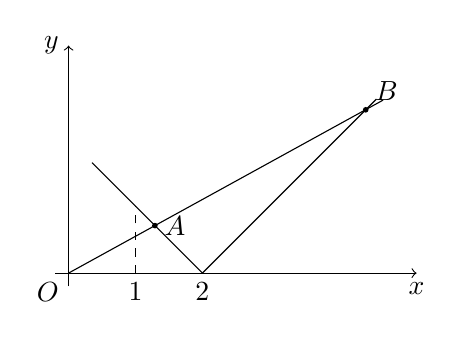
\begin{tikzpicture}[scale=0.85]
\draw[->] (-0.2,0) -- (5.2,0) node[below]{$x$};
\draw[->] (0,-0.2) -- (0,3.4) node[left]{$y$};
\node[below left] at (0,0) {$O$};
\draw (2,0) -- (0.35,1.65);
\draw (2,0) -- (4.6,2.6);
\draw (0,0) -- (4.7,2.585);
\draw[dashed] (1,0) -- (1,1);
\node[below] at (1,0) {$1$};
\node[below] at (2,0) {$2$};
\coordinate (A) at (1.29,0.71); \fill (A) circle (1.2pt); \node[right] at (A) {$A$};
\coordinate (B) at (4.44,2.44); \fill (B) circle (1.2pt); \node[above right] at (B) {$B$};
\end{tikzpicture}
\end{center}
\step{由 $0<k<1$，得 $x_A>1$，}
\step{所以关于 $x$ 的不等式 $k\lvert x\rvert-\lvert x-2\rvert>0$ 恰好有 $4$ 个整数解，是 $2,3,4,5$，}
\step{由 $\begin{cases}y=kx\\ y=x-2\end{cases}\Rightarrow x_B=\dfrac2{1-k}\in(5,6]$，故 $\dfrac35<k\leqslant\dfrac23$.}
\solend
\fi

\item 设集合 $S=\{1,2,3,\cdots,10\}$，$S$ 的子集 $A$ 满足 $A\cap\{1,2,3\}\neq\varnothing$，$A\cup\{4,5,6\}\neq S$，这样的子集 $A$ 的个数为\blankline[4.4em].

\ifanswer
\solbegin
\step{先求使 $A\cap\{1,2,3\}\neq\varnothing$ 成立的 $S$ 的子集 $A$ 的个数 $N_1$，}
\step{在 $\{1,2,3\}$ 中取出至少一个元素的方式有 $7$ 种，}
\step{而集合 $\{4,5,\cdots,10\}$ 的子集有 $2^7$ 个，因此 $N_1=7\times2^7=896$，}
% 注：下一行原卷印作“$A\cup\{4,5,6\}\neq S$”，按上下文应为“$=S$”，照录未改（见文件头“原卷笔误/存疑”①）。
\step{再扣除其中使 $A\cup\{4,5,6\}\neq S$ 的集合 $A$ 的个数 $N_2$，}
\step{这些取法中 $1$，$2$，$3$，$7$，$8$，$9$，$10$ 均被取出，}
\step{而集合 $\{4,5,6\}$ 的子集有 $2^3$ 个，因此 $N_2=2^3=8$，}
\step{从而满足条件的子集 $A$ 的个数为 $N_1-N_2=896-8=888$.}
\solend
\fi

\end{enumerate}

\bigsec{二、选择题}

\begin{enumerate}
\setcounter{enumi}{12}

\item 已知 $a>b$，下列不等式中一定成立是\mbox{（\quad）}

\keepwithprev
A. $a^2>b^2$\qquad B. $ac^2>bc^2$\qquad C. $\dfrac1a<\dfrac1b$\qquad D. $a+3>b-4$

\ifanswer
\solbegin
\step{对于 $A$，当 $a=-2$，$b=-4$ 时，不等式不成立，故 $A$ 错误；}
\step{对于 $B$，当 $c=0$ 时，不等式不成立，故 $B$ 错误；}
\step{对于 $C$，当 $a=2$，$b=-4$ 时，不等式不成立，故 $C$ 错误；}
\step{对于 $D$，因为 $a>b$，$3>-4$，必有 $a+3>b-4$ 成立，故 $D$ 正确.}
\solend
\fi

\item 已知集合 $M$ 满足 $\{2,3\}\subseteq M\subseteq\{1,2,3,4,5\}$，那么这样的集合 $M$ 的个数为\mbox{（\quad）}

\keepwithprev
A. $6$\qquad B. $7$\qquad C. $8$\qquad D. $9$

\ifanswer
\solbegin
\step{集合 $M$ 满足 $\{2,3\}\subseteq M\subseteq\{1,2,3,4,5\}$，所以 $2\in M$，$3\in M$，}
\step{故集合 $M$ 的个数为 $2^3=8$. 故选 $C$.}
\solend
\fi

\item 已知集合 $A=\{x\mid x=2k,k\in\Z\}$，$B=\{x\mid x=4m+6n,m,n\in\Z\}$，则\mbox{（\quad）}

\keepwithprev
A. $B\subset A$\qquad B. $A\subset B$\qquad C. $A=B$\qquad D. $B\neq A$

\ifanswer
\solbegin
\step{$B=\{x\mid x=4m+6n,m,n\in\Z\}$，$B$ 中的元素都是偶数，}
\step{所以 $B$ 的元素都是 $A$ 的元素，$B\subseteq A$；}
\step{$A=\{x\mid x=4(-k)+6k,k\in\Z\}$，则 $A$ 的元素都是 $B$ 的元素，$A\subseteq B$；}
\step{所以 $A=B$. 故选 $C$.}
\solend
\fi

\item 已知集合 $A=[1,a]\cup[a^3,a^4]$，集合 $B=\{x\mid x=x_1-x_2$，其中 $x_1,x_2\in A\}$. 若集合 $B$ 表示的区间为一个闭区间，则 $a$ 的取值范围为\mbox{（\quad）}

\keepwithprev
A. $a$ 取遍任意大于 $1$ 的实数\qquad B. $a\geqslant2$

C. $a\geqslant\dfrac{1+\sqrt5}2$\qquad D. $a\geqslant1+\sqrt2$

\ifanswer
\solbegin
\step{由题意得 $a^3>a>1$，则 $x_1-x_2$ 的最小值为 $1-a^4$，最大值为 $a^4-1$，}
\step{所以 $B=[1-a^4,a^4-1]$，}
\step{又因为 $a^4-a^3-(a-1)=a^3(a-1)-(a-1)=(a^3-1)(a-1)>0$，}
\step{所以 $a^4-a^3>a-1$，又集合 $B$ 表示的区间为一个闭区间，}
\step{则 $a^3-a\leqslant a^4-a^3$，化简得 $a^2-a-1\geqslant0$，又 $a>1$，解得 $a\geqslant\dfrac{1+\sqrt5}2$.}
\step{故选 $C$.}
\solend
\fi

\end{enumerate}

\bigsec{三、解答题}

\begin{enumerate}
\setcounter{enumi}{16}

\item 设全集 $U=\R$，集合 $A=\{x\mid\lvert x+3\rvert\leqslant4\}$，集合 $B=\{x\mid a-2\leqslant x\leqslant1+2a\}$，其中 $a\in\R$.

（1）若 $a=\dfrac12$，求 $A\cap B$；

（2）若 $A\cap B=\varnothing$，求 $a$ 的取值范围.

\ifanswer
\solbegin
\stepm{(1)}{由 $\lvert x+3\rvert\leqslant4$，得 $-4\leqslant x+3\leqslant4$，解得 $-7\leqslant x\leqslant1$，}
\step{所以 $A=\{x\mid-7\leqslant x\leqslant1\}$，}
\step{当 $a=\dfrac12$ 时，$a-2=\dfrac12-2=-\dfrac32$，$1+2a=1+2\times\dfrac12=2$，}
\step{$B=\left\{x\mid-\dfrac32\leqslant x\leqslant2\right\}$，$A\cap B=\left\{x\mid-\dfrac32\leqslant x\leqslant1\right\}$，即 $\left[-\dfrac32,1\right]$.}
\stepm{(2)}{若 $A\cap B=\varnothing$，分两种情况讨论，}
\step{①当 $B\neq\varnothing$ 时，$a-2\leqslant1+2a$，即 $a\geqslant-3$，}
\step{要满足 $A\cap B=\varnothing$，则 $1+2a<-7$ 或 $a-2>1$，}
\step{由 $1+2a<-7$，得 $a<-4$，与 $a\geqslant-3$ 无交集，无解，}
\step{由 $a-2>1$ 得 $a>3$，符合 $a\geqslant-3$，}
\step{②当 $B=\varnothing$ 时，有 $a-2>1+2a$，解得 $a<-3$，满足 $A\cap B=\varnothing$；}
\step{综上，$a$ 的取值范围是 $(-\infty,-3)\cup(3,+\infty)$.}
\solend
\fi

\ansspace

\item （1）已知 $a>b>0$，比较 $\dfrac{a+b}{a^2+b^2}$ 与 $\dfrac1{a-b}$ 的大小并说明理由；

（2）已知 $-2\leqslant x\leqslant-1$，$2\leqslant y\leqslant3$，求 $2x-y$ 的取值范围.

\ifanswer
\solbegin
\stepm{(1)}{$\dfrac{a+b}{a^2+b^2}-\dfrac1{a-b}=\dfrac{(a^2-b^2)-(a^2+b^2)}{(a^2+b^2)(a-b)}=\dfrac{-2b^2}{(a^2+b^2)(a-b)}$，}
\step{因为 $a>b>0$，所以 $a^2(a-b)-b^2(b-a)=(a^2+b^2)(a-b)>0$，}
\step{$\dfrac{-2b^2}{(a^2+b^2)(a-b)}<0$，即 $\dfrac{a+b}{a^2+b^2}-\dfrac1{a-b}<0$，所以 $\dfrac{a+b}{a^2+b^2}<\dfrac1{a-b}$；}
\stepm{(2)}{由 $-2\leqslant x\leqslant-1$，$2\leqslant y\leqslant3$，得 $-4\leqslant2x\leqslant-2$，$-3\leqslant-y\leqslant-2$，}
\step{得 $-7\leqslant2x-y\leqslant-4$，即 $2x-y$ 的取值范围为 $[-7,-4]$.}
\solend
\fi

\ansspace

\item 设 $x_1$、$x_2$ 是关于 $x$ 的方程 $x^2-2(m+2)x+m^2-1=0$ 的两个实数根.

（1）若 $\dfrac1{x_1}+\dfrac1{x_2}=-4$，求 $m$ 的值；

（2）若 $x_1$、$x_2$ 是两个不相等的正数，求实数 $m$ 的取值范围.

\ifanswer
\solbegin
\stepm{(1)}{因为 $x_1$、$x_2$ 是关于 $x$ 的方程的两个实数根，}
\step{所以 $\Delta=(-2(m+2))^2-4(m^2-1)=16m+20\geqslant0$，解得 $m\geqslant-\dfrac54$，}
\step{由韦达定理得 $x_1+x_2=2(m+2)$，$x_1x_2=m^2-1$，}
\step{所以 $\dfrac1{x_1}+\dfrac1{x_2}=\dfrac{x_2+x_1}{x_1x_2}=\dfrac{2(m+2)}{m^2-1}=-4$，即 $2m^2+m=0$，}
\step{解得 $m=0$ 或 $m=-\dfrac12$；}
\stepm{(2)}{由题意得 $\begin{cases}x_1+x_2>0\\ x_1x_2>0\\ \Delta>0\end{cases}$，即 $\begin{cases}2(m+2)>0\\ m^2-1>0\\ (-2(m+2))^2-4(m^2-1)>0\end{cases}$，}
\step{解得 $-\dfrac54<m<-1$ 或 $m>1$.}
\solend
\fi

\ansspace

\ifanswer\else\needvspace{10\baselineskip}\fi
\item 已知集合 $A=\{x\mid x\leqslant2\text{ 或 }x\geqslant a\}$.

（1）若 $B=\left\{x\mid(x-2)\left(x-\dfrac{12}{7-a}\right)<0\right\}$，$A\cap B=\varnothing$，$A\cup B=\R$，求实数 $a$ 的值；

（2）若 $a=3$ 且 $b<2$，$B=\{x\mid x^2-b(b+1)x+b^3<0\}$，$A\cap B\cap\Z$ 的子集个数为 $4$ 个，求实数 $b$ 的取值范围.

\ifanswer
\solbegin
\stepm{(1)}{当 $a\leqslant2$ 时，$A=\{x\mid x\leqslant2\text{ 或 }x\geqslant a\}=\R$，必有 $B=\varnothing$，}
\step{即不等式 $(x-2)\left(x-\dfrac{12}{7-a}\right)<0$ 无解，}
\step{必有 $\dfrac{12}{7-a}=2$，解得 $a=1$，符合题意，}
\step{当 $a>2$ 时，$A=(-\infty,2]\cup[a,+\infty)$，}
\step{若 $A\cap B=\varnothing$，$A\cup B=\R$，则 $B=(2,a)$，}
\step{即方程 $(x-2)\left(x-\dfrac{12}{7-a}\right)=0$ 的两个根是 $2$ 和 $a$，所以 $\dfrac{12}{7-a}=a$，}
\step{解得 $a=3$ 或 $a=4$，符合题意，}
\step{综上，实数 $a$ 的值为 $1$ 或 $3$ 或 $4$；}
\stepm{(2)}{由 $A\cap B\cap\Z$ 的子集个数为 $4$ 个，即 $A\cap B\cap\Z$ 中恰好有 $2$ 个整数元素，}
\step{由 $a=3$，则 $A=(-\infty,2]\cup[3,+\infty)$，}
\step{由 $x^2-b(b+1)x+b^3=(x-b^2)(x-b)<0$，又 $b<2$，}
\step{当 $1<b<2$ 时，$1<b^2<4$ 且 $b^2>b$，则 $B=(b,b^2)$，}
\step{则 $A\cap B=(b,2]\cup[3,b^2)$，}
\step{要使 $A\cap B\cap\Z$ 中恰好有 $2$ 个整数元素，即 $A\cap B\cap\Z=\{2,3\}$，}
\step{即 $\begin{cases}1<b<2\\ 3<b^2<4\end{cases}$，解得 $\sqrt3<b<2$，符合题意，}
\step{当 $b=1$ 或 $b=0$ 时，$B=\varnothing$，此时 $A\cap B\cap\Z=\varnothing$，不符合题意，舍去，}
\step{当 $0<b<1$ 时，$0<b^2<1$ 且 $b^2<b$，则 $B=(b^2,b)$，}
\step{此时 $A\cap B\cap\Z=\varnothing$，不符合题意，舍去，}
\step{当 $-1<b<0$ 时，$0<b^2<1$ 且 $b^2>b$，则 $B=(b,b^2)$，}
\step{此时 $A\cap B\cap\Z=\{0\}$，即 $A\cap B\cap\Z$ 中只有 $1$ 个元素，不符合题意，舍去，}
\step{当 $b\leqslant-1$ 时，$b^2\geqslant1$ 且 $b^2>b$，则 $B=(b,b^2)$，}
\step{此时 $A\cap B\cap\Z\supseteq\{-1,0,1\}$，即 $A\cap B\cap\Z$ 中至少有 $3$ 个元素，}
\step{不符合题意，舍去，}
\step{综上，实数 $b$ 的取值范围为 $(\sqrt3,2)$.}
\solend
\fi

\ansspace*[7]

\item 已知集合 $A=\{a_1,a_2,a_3,\cdots,a_n\}$ 中的元素均为正整数，其中 $n\in\N$ 且 $n\geqslant3$. 若对任意 $x,y\in A(x\neq y)$，都有 $\lvert x-y\rvert\geqslant\dfrac{xy}k$，则称集合 $A$ 具有性质 $M_k$.

（1）集合 $A=\{1,2,a\}$ 具有性质 $M_3$，求 $a$ 的最小值；

（2）若集合 $A$ 具有性质 $M_{24}$，且 $A$ 中最小元素和最大元素分别为 $a,b$，求证：$\dfrac1a-\dfrac1b\geqslant\dfrac{n-1}{24}$；

（3）已知集合 $A$ 具有性质 $M_{24}$，求 $A$ 中元素个数的最大值，并说明理由.

\ifanswer
\solbegin
\stepm{(1)}{由性质 $M_3$ 定义得 $\begin{cases}a-1\geqslant\dfrac a3\\ a-2\geqslant\dfrac{2a}3\end{cases}\Rightarrow\begin{cases}a\geqslant\dfrac32\\ a\geqslant6\end{cases}\Rightarrow a\geqslant6$，且 $a\subseteq\N^*$，}
% 注：上一行原卷印作“$a\subseteq\N^*$”，应为“$a\in\N^*$”，照录未改（见文件头“原卷笔误/存疑”②）。
\step{所以 $a$ 的最小值为 $6$.}
\stepm{(2)}{由题意得 $\lvert a_i-a_{i+1}\rvert\geqslant\dfrac{a_ia_{i+1}}{24}$，$(i=1,2,3,\cdots,n-1)$，且 $a_1<\cdots<a_n$，}
\step{所以 $a_{i+1}-a_i\geqslant\dfrac{a_ia_{i+1}}{24}\Rightarrow\dfrac1{a_i}-\dfrac1{a_{i+1}}\geqslant\dfrac1{24}$，$(i=1,2,3,\cdots,n-1)$，}
\step{所以 $\dfrac1{a_1}-\dfrac1{a_2}+\dfrac1{a_2}-\dfrac1{a_3}+\cdots+\dfrac1{a_{n-1}}-\dfrac1{a_n}=\dfrac1{a_1}-\dfrac1{a_n}\geqslant\dfrac{n-1}{24}$，得证.}
\stepm{(3)}{由 (2) 得 $\begin{cases}\dfrac1{a_1}\geqslant\dfrac{n-1}{24}\\ a_1\geqslant1\end{cases}\Rightarrow\dfrac{n-1}{24}<1\Rightarrow n<25$，}
\step{同 (2) 证明得 $\dfrac1{a_i}-\dfrac1{a_n}\geqslant\dfrac{n-i}{24}$ 且 $i=1,2,3,\cdots,n-1$，故 $\dfrac1{a_i}>\dfrac{n-i}{24}$，}
\step{又 $a_i\geqslant i$，所以 $\dfrac1i>\dfrac{n-i}{24}\Rightarrow i(n-i)<24$ 在 $i=1,2,3,\cdots,n-1$ 上恒成立，}
\step{当 $n\geqslant10$，取 $i=5$，则 $i(n-i)=5(n-5)>24$，故 $n<10$，}
\step{当 $n\leqslant9$，则 $i(n-i)\leqslant\dfrac{(i+n-i)^2}4=\dfrac{n^2}4<24\Rightarrow n<\sqrt{96}$，即 $n\leqslant9$.}
\step{综上，集合 $A$ 中元素个数的最大值为 $9$.}
\solend
\fi

\end{enumerate}

\end{document}
"
% 紧凑版：xelatex "\def\iscompact{1}% 高一79_南汇中学_10月月考.tex
%   —— 高一上数学“2026-2027 年南汇中学高一上 10 月月考”（讲评版）
% 试卷版：xelatex 高一79_南汇中学_10月月考.tex
% 答案版：xelatex "\def\isanswer{1}\input{高一79_南汇中学_10月月考.tex}"
% 紧凑版：xelatex "\def\iscompact{1}\input{高一79_南汇中学_10月月考.tex}"
%
% 原始材料：微信公众号“魔都数学加油站”文章，连载“27学年高一79”；
% 原文标题“27学年高一79——2026-2027年上海市南汇中学高一上10月月考”；
% 原文链接：https://mp.weixin.qq.com/s/bFvc7GVgPTaDGg_6JSSfGg。
% 页面标注发布时间 2026-10-24 21:00（上海）。
% 正文为 9 张 PNG 页（`原图/高一79_南汇中学_10月月考/01..09.png`），
% 尺寸混排（第 1、2、4、5、7、8 页为 4762×6735，第 3、6、9 页为 2560×3620），均按页序读取。
%
% 篇幅与题号：原卷自第 3 题起编号。填空题 3—12（10 题）、选择题 13—16（4 题）、
% 解答题 17—21（5 题），共 19 题。
%
% 讲评版：第 4 题只印【答案】，本稿只给 \ans{}；其余 18 题印【解析】。
% 选择题答案在解析末句“故选 D／C／C／C”。
%
% 副标题：原卷未印副标题。本稿按内容标作“集合与常用逻辑用语、不等式”。
%
% 原卷笔误/存疑（均照录未改，正文对应处另有 % 注）：
%   ① 第 12 题解析作“再扣除其中使 $A\cup\{4,5,6\}\neq S$ 的集合 $A$ 的个数 $N_2$”，
%      按上下文应为“$A\cup\{4,5,6\}=S$”，否则“这些取法中 $1,2,3,7,8,9,10$ 均被取出”
%      与 $N_2=2^3=8$ 都无法解释；原卷印作 $\neq$，照录未改。
%   ② 第 21 题 (1) 解析末作“且 $a\subseteq\N^*$”，$a$ 是集合的元素，应为 $a\in\N^*$；
%      原卷印作 $\subseteq$，照录未改。
%
% 与原卷的排版差异：
%   ① 原卷每题下直接印【答案】/【解析】，本稿按全稿惯例将答案与解析置于答案版；
%   ② 原卷未印副标题，本稿补出；填空横线统一排 \blankline[4.4em]；
%   ③ 原卷数集记号排斜体 $R$、$Z$、$N$，本稿按全稿惯例改用 $\R$、$\Z$、$\N$；
%   ④ 第 17—21 题的子问用行内“（1）（2）（3）”段，解析中的子问标号用 \stepm；
%   ⑤ 解答题按惯例加 \ansspace；选择题括号排 \mbox{（\quad）}；
%   ⑥ 第 11 题解析有一幅函数图象（$y=k\lvert x\rvert$ 与 $y=\lvert x-2\rvert$），
%      按原图形状用 TikZ 重排（仅答案版出）。
%
% 行数核对：逐题数 \step/\stepm 条数，合计 107 条（Q3：2；Q5：2；Q6：1；Q7：4；Q8：4；
% Q9：4；Q10：5；Q11：4；Q12：7；Q13：4；Q14：2；Q15：4；Q16：6；Q17：11；Q18：5；
% Q19：7；Q20：24；Q21：11）。原卷解析的换行按语意合并，未逐行强拆；第 4 题只印
% 【答案】，提 \ans{}，不计入 \step 账。
%
\documentclass[a4paper,11pt]{article}
\usepackage{common}

\begin{document}

\examtitlest[3]{2026--2027 年南汇中学高一上 10 月月考}{集合与常用逻辑用语、不等式}

\bigsec{一、填空题}

\begin{enumerate}
\setcounter{enumi}{2}

\item 不等式 $\dfrac{1-x}{x}>0$ 的解集为\blankline[4.4em].

\ifanswer
\solbegin
\step{原不等式化为 $x(x-1)<0$，转化为 $\begin{cases}x>0\\ x-1<0\end{cases}$ 或 $\begin{cases}x<0\\ x-1>0\end{cases}$，}
\step{解得 $0<x<1$，则不等式的解集为 $\{x\mid0<x<1\}$.}
\solend
\fi

\item 用反证法证明命题：“若 $x^2<1$，则 $-1<x<1$”时，应假设\blankline[4.4em].

\ifanswer
\ans{$x\geqslant1$ 或 $x\leqslant-1$}
\fi

\item 设 $k$ 为实数，关于 $x$ 的不等式 $kx^2+x+2<0$ 的解集为 $A$，若 $2\notin A$，则 $k$ 的取值范围是\blankline[4.4em].

\ifanswer
\solbegin
\step{因为关于 $x$ 的不等式 $kx^2+x+2<0$ 的解集为 $A$，且 $2\notin A$，}
\step{所以 $x=2$ 时，$k\times2^2+2+2\geqslant0$，解得 $k\geqslant-1$，则 $k$ 的取值范围为 $[-1,+\infty)$.}
\solend
\fi

\item 已知集合 $M=\{y\mid y=x^2-2x,x\in\R\}$，$N=\{x\mid y=\sqrt{4-x^2}\}$，则 $M\cup N=$\blankline[4.4em].

\ifanswer
\solbegin
\step{$M=[-1,+\infty)$，$N=[-2,2]$，则 $M\cup N=[-2,+\infty)$.}
\solend
\fi

\item 设集合 $A=\{-3,2\}$，集合 $B=\{x\mid mx+1=0\}$，且 $A\cup B=A$，则 $m$ 的值组成的集合是\blankline[4.4em].

\ifanswer
\solbegin
\step{由 $A\cup B=A$，得 $B\subseteq A$，}
\step{当 $m=0$ 时，$B=\varnothing$，满足题意，}
\step{当 $m\neq0$ 时，$B=\left\{-\dfrac1m\right\}$，所以 $-\dfrac1m=2$ 或 $-\dfrac1m=-3$，所以 $m=-\dfrac12$ 或 $m=\dfrac13$，}
\step{综上所述，$m$ 的值组成的集合是 $\left\{0,-\dfrac12,\dfrac13\right\}$.}
\solend
\fi

\item 若不等式 $\lvert x\rvert<a$ 的一个充分不必要条件为 $\dfrac{2x-1}{x-2}<1$，则实数 $a$ 的取值范围是\blankline[4.4em].

\ifanswer
\solbegin
\step{不等式 $\lvert x\rvert<a$，得 $-a<x<a$，}
\step{不等式 $\dfrac{2x-1}{x-2}<1$，即 $\dfrac{2x-1-(x-2)}{x-2}=\dfrac{x+1}{x-2}<0$，解得 $-1<x<2$，}
\step{又不等式 $\lvert x\rvert<a$ 的一个充分不必要条件为 $\dfrac{2x-1}{x-2}<1$，}
\step{得 $\begin{cases}a\geqslant2\\ -a\leqslant-1\end{cases}$，且两等号不同时成立，解得 $a\geqslant2$.}
\solend
\fi

\item 若对任意 $x\in\R$ 都有 $(m-1)x^2-(m-1)x-1<0$，则实数 $m$ 的取值范围是\blankline[4.4em].

\ifanswer
\solbegin
\step{当 $m-1\neq0$，即 $m\neq1$ 时，则有 $\begin{cases}m-1<0\\ (m-1)^2-4(m-1)\times(-1)<0\end{cases}$，}
\step{解得 $-3<m<1$；}
\step{当 $m-1=0$ 时，即当 $m=1$ 时，此时不等式为 $-1<0$ 恒成立，符合题意；}
\step{综上所述，实数 $m$ 的取值范围是 $(-3,1]$.}
\solend
\fi

\item 关于 $x$ 的方程 $\dfrac{x}{x-1}=\dfrac{k-x}{x^2-x}$ 的解集中只含有一个元素，则 $k$ 的可能取值构成的集合为\blankline[4.4em].

\ifanswer
\solbegin
\step{方程两边同时乘以 $x(x-1)$ 得 $x^2=k-x$，即 $x^2+x-k=0$，}
\step{①当其中一个解为增根时，方程也只有一个解，}
\step{(i) 若增根为 $0$ 时，$k=0$；(ii) 若增根为 $1$ 时，$k=2$；}
\step{②当 $\Delta=1+4k=0$，即 $k=-\dfrac14$ 时，方程 $x^2+x-k=0$ 只有一个解；}
\step{即 $k$ 的可能取值构成的集合为 $\left\{-\dfrac14,0,2\right\}$.}
\solend
\fi

\item 若关于 $x$ 的不等式 $k\lvert x\rvert>\lvert x-2\rvert$ 恰好有 $4$ 个整数解，则实数 $k$ 的取值范围是\blankline[4.4em].

\ifanswer
\solbegin
\step{由题意得 $0<k<1$，函数 $y=k\lvert x\rvert$ 与 $y=\lvert x-2\rvert$ 的图象如图：}
\begin{center}
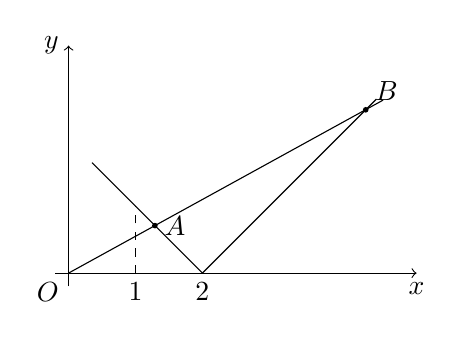
\begin{tikzpicture}[scale=0.85]
\draw[->] (-0.2,0) -- (5.2,0) node[below]{$x$};
\draw[->] (0,-0.2) -- (0,3.4) node[left]{$y$};
\node[below left] at (0,0) {$O$};
\draw (2,0) -- (0.35,1.65);
\draw (2,0) -- (4.6,2.6);
\draw (0,0) -- (4.7,2.585);
\draw[dashed] (1,0) -- (1,1);
\node[below] at (1,0) {$1$};
\node[below] at (2,0) {$2$};
\coordinate (A) at (1.29,0.71); \fill (A) circle (1.2pt); \node[right] at (A) {$A$};
\coordinate (B) at (4.44,2.44); \fill (B) circle (1.2pt); \node[above right] at (B) {$B$};
\end{tikzpicture}
\end{center}
\step{由 $0<k<1$，得 $x_A>1$，}
\step{所以关于 $x$ 的不等式 $k\lvert x\rvert-\lvert x-2\rvert>0$ 恰好有 $4$ 个整数解，是 $2,3,4,5$，}
\step{由 $\begin{cases}y=kx\\ y=x-2\end{cases}\Rightarrow x_B=\dfrac2{1-k}\in(5,6]$，故 $\dfrac35<k\leqslant\dfrac23$.}
\solend
\fi

\item 设集合 $S=\{1,2,3,\cdots,10\}$，$S$ 的子集 $A$ 满足 $A\cap\{1,2,3\}\neq\varnothing$，$A\cup\{4,5,6\}\neq S$，这样的子集 $A$ 的个数为\blankline[4.4em].

\ifanswer
\solbegin
\step{先求使 $A\cap\{1,2,3\}\neq\varnothing$ 成立的 $S$ 的子集 $A$ 的个数 $N_1$，}
\step{在 $\{1,2,3\}$ 中取出至少一个元素的方式有 $7$ 种，}
\step{而集合 $\{4,5,\cdots,10\}$ 的子集有 $2^7$ 个，因此 $N_1=7\times2^7=896$，}
% 注：下一行原卷印作“$A\cup\{4,5,6\}\neq S$”，按上下文应为“$=S$”，照录未改（见文件头“原卷笔误/存疑”①）。
\step{再扣除其中使 $A\cup\{4,5,6\}\neq S$ 的集合 $A$ 的个数 $N_2$，}
\step{这些取法中 $1$，$2$，$3$，$7$，$8$，$9$，$10$ 均被取出，}
\step{而集合 $\{4,5,6\}$ 的子集有 $2^3$ 个，因此 $N_2=2^3=8$，}
\step{从而满足条件的子集 $A$ 的个数为 $N_1-N_2=896-8=888$.}
\solend
\fi

\end{enumerate}

\bigsec{二、选择题}

\begin{enumerate}
\setcounter{enumi}{12}

\item 已知 $a>b$，下列不等式中一定成立是\mbox{（\quad）}

\keepwithprev
A. $a^2>b^2$\qquad B. $ac^2>bc^2$\qquad C. $\dfrac1a<\dfrac1b$\qquad D. $a+3>b-4$

\ifanswer
\solbegin
\step{对于 $A$，当 $a=-2$，$b=-4$ 时，不等式不成立，故 $A$ 错误；}
\step{对于 $B$，当 $c=0$ 时，不等式不成立，故 $B$ 错误；}
\step{对于 $C$，当 $a=2$，$b=-4$ 时，不等式不成立，故 $C$ 错误；}
\step{对于 $D$，因为 $a>b$，$3>-4$，必有 $a+3>b-4$ 成立，故 $D$ 正确.}
\solend
\fi

\item 已知集合 $M$ 满足 $\{2,3\}\subseteq M\subseteq\{1,2,3,4,5\}$，那么这样的集合 $M$ 的个数为\mbox{（\quad）}

\keepwithprev
A. $6$\qquad B. $7$\qquad C. $8$\qquad D. $9$

\ifanswer
\solbegin
\step{集合 $M$ 满足 $\{2,3\}\subseteq M\subseteq\{1,2,3,4,5\}$，所以 $2\in M$，$3\in M$，}
\step{故集合 $M$ 的个数为 $2^3=8$. 故选 $C$.}
\solend
\fi

\item 已知集合 $A=\{x\mid x=2k,k\in\Z\}$，$B=\{x\mid x=4m+6n,m,n\in\Z\}$，则\mbox{（\quad）}

\keepwithprev
A. $B\subset A$\qquad B. $A\subset B$\qquad C. $A=B$\qquad D. $B\neq A$

\ifanswer
\solbegin
\step{$B=\{x\mid x=4m+6n,m,n\in\Z\}$，$B$ 中的元素都是偶数，}
\step{所以 $B$ 的元素都是 $A$ 的元素，$B\subseteq A$；}
\step{$A=\{x\mid x=4(-k)+6k,k\in\Z\}$，则 $A$ 的元素都是 $B$ 的元素，$A\subseteq B$；}
\step{所以 $A=B$. 故选 $C$.}
\solend
\fi

\item 已知集合 $A=[1,a]\cup[a^3,a^4]$，集合 $B=\{x\mid x=x_1-x_2$，其中 $x_1,x_2\in A\}$. 若集合 $B$ 表示的区间为一个闭区间，则 $a$ 的取值范围为\mbox{（\quad）}

\keepwithprev
A. $a$ 取遍任意大于 $1$ 的实数\qquad B. $a\geqslant2$

C. $a\geqslant\dfrac{1+\sqrt5}2$\qquad D. $a\geqslant1+\sqrt2$

\ifanswer
\solbegin
\step{由题意得 $a^3>a>1$，则 $x_1-x_2$ 的最小值为 $1-a^4$，最大值为 $a^4-1$，}
\step{所以 $B=[1-a^4,a^4-1]$，}
\step{又因为 $a^4-a^3-(a-1)=a^3(a-1)-(a-1)=(a^3-1)(a-1)>0$，}
\step{所以 $a^4-a^3>a-1$，又集合 $B$ 表示的区间为一个闭区间，}
\step{则 $a^3-a\leqslant a^4-a^3$，化简得 $a^2-a-1\geqslant0$，又 $a>1$，解得 $a\geqslant\dfrac{1+\sqrt5}2$.}
\step{故选 $C$.}
\solend
\fi

\end{enumerate}

\bigsec{三、解答题}

\begin{enumerate}
\setcounter{enumi}{16}

\item 设全集 $U=\R$，集合 $A=\{x\mid\lvert x+3\rvert\leqslant4\}$，集合 $B=\{x\mid a-2\leqslant x\leqslant1+2a\}$，其中 $a\in\R$.

（1）若 $a=\dfrac12$，求 $A\cap B$；

（2）若 $A\cap B=\varnothing$，求 $a$ 的取值范围.

\ifanswer
\solbegin
\stepm{(1)}{由 $\lvert x+3\rvert\leqslant4$，得 $-4\leqslant x+3\leqslant4$，解得 $-7\leqslant x\leqslant1$，}
\step{所以 $A=\{x\mid-7\leqslant x\leqslant1\}$，}
\step{当 $a=\dfrac12$ 时，$a-2=\dfrac12-2=-\dfrac32$，$1+2a=1+2\times\dfrac12=2$，}
\step{$B=\left\{x\mid-\dfrac32\leqslant x\leqslant2\right\}$，$A\cap B=\left\{x\mid-\dfrac32\leqslant x\leqslant1\right\}$，即 $\left[-\dfrac32,1\right]$.}
\stepm{(2)}{若 $A\cap B=\varnothing$，分两种情况讨论，}
\step{①当 $B\neq\varnothing$ 时，$a-2\leqslant1+2a$，即 $a\geqslant-3$，}
\step{要满足 $A\cap B=\varnothing$，则 $1+2a<-7$ 或 $a-2>1$，}
\step{由 $1+2a<-7$，得 $a<-4$，与 $a\geqslant-3$ 无交集，无解，}
\step{由 $a-2>1$ 得 $a>3$，符合 $a\geqslant-3$，}
\step{②当 $B=\varnothing$ 时，有 $a-2>1+2a$，解得 $a<-3$，满足 $A\cap B=\varnothing$；}
\step{综上，$a$ 的取值范围是 $(-\infty,-3)\cup(3,+\infty)$.}
\solend
\fi

\ansspace

\item （1）已知 $a>b>0$，比较 $\dfrac{a+b}{a^2+b^2}$ 与 $\dfrac1{a-b}$ 的大小并说明理由；

（2）已知 $-2\leqslant x\leqslant-1$，$2\leqslant y\leqslant3$，求 $2x-y$ 的取值范围.

\ifanswer
\solbegin
\stepm{(1)}{$\dfrac{a+b}{a^2+b^2}-\dfrac1{a-b}=\dfrac{(a^2-b^2)-(a^2+b^2)}{(a^2+b^2)(a-b)}=\dfrac{-2b^2}{(a^2+b^2)(a-b)}$，}
\step{因为 $a>b>0$，所以 $a^2(a-b)-b^2(b-a)=(a^2+b^2)(a-b)>0$，}
\step{$\dfrac{-2b^2}{(a^2+b^2)(a-b)}<0$，即 $\dfrac{a+b}{a^2+b^2}-\dfrac1{a-b}<0$，所以 $\dfrac{a+b}{a^2+b^2}<\dfrac1{a-b}$；}
\stepm{(2)}{由 $-2\leqslant x\leqslant-1$，$2\leqslant y\leqslant3$，得 $-4\leqslant2x\leqslant-2$，$-3\leqslant-y\leqslant-2$，}
\step{得 $-7\leqslant2x-y\leqslant-4$，即 $2x-y$ 的取值范围为 $[-7,-4]$.}
\solend
\fi

\ansspace

\item 设 $x_1$、$x_2$ 是关于 $x$ 的方程 $x^2-2(m+2)x+m^2-1=0$ 的两个实数根.

（1）若 $\dfrac1{x_1}+\dfrac1{x_2}=-4$，求 $m$ 的值；

（2）若 $x_1$、$x_2$ 是两个不相等的正数，求实数 $m$ 的取值范围.

\ifanswer
\solbegin
\stepm{(1)}{因为 $x_1$、$x_2$ 是关于 $x$ 的方程的两个实数根，}
\step{所以 $\Delta=(-2(m+2))^2-4(m^2-1)=16m+20\geqslant0$，解得 $m\geqslant-\dfrac54$，}
\step{由韦达定理得 $x_1+x_2=2(m+2)$，$x_1x_2=m^2-1$，}
\step{所以 $\dfrac1{x_1}+\dfrac1{x_2}=\dfrac{x_2+x_1}{x_1x_2}=\dfrac{2(m+2)}{m^2-1}=-4$，即 $2m^2+m=0$，}
\step{解得 $m=0$ 或 $m=-\dfrac12$；}
\stepm{(2)}{由题意得 $\begin{cases}x_1+x_2>0\\ x_1x_2>0\\ \Delta>0\end{cases}$，即 $\begin{cases}2(m+2)>0\\ m^2-1>0\\ (-2(m+2))^2-4(m^2-1)>0\end{cases}$，}
\step{解得 $-\dfrac54<m<-1$ 或 $m>1$.}
\solend
\fi

\ansspace

\ifanswer\else\needvspace{10\baselineskip}\fi
\item 已知集合 $A=\{x\mid x\leqslant2\text{ 或 }x\geqslant a\}$.

（1）若 $B=\left\{x\mid(x-2)\left(x-\dfrac{12}{7-a}\right)<0\right\}$，$A\cap B=\varnothing$，$A\cup B=\R$，求实数 $a$ 的值；

（2）若 $a=3$ 且 $b<2$，$B=\{x\mid x^2-b(b+1)x+b^3<0\}$，$A\cap B\cap\Z$ 的子集个数为 $4$ 个，求实数 $b$ 的取值范围.

\ifanswer
\solbegin
\stepm{(1)}{当 $a\leqslant2$ 时，$A=\{x\mid x\leqslant2\text{ 或 }x\geqslant a\}=\R$，必有 $B=\varnothing$，}
\step{即不等式 $(x-2)\left(x-\dfrac{12}{7-a}\right)<0$ 无解，}
\step{必有 $\dfrac{12}{7-a}=2$，解得 $a=1$，符合题意，}
\step{当 $a>2$ 时，$A=(-\infty,2]\cup[a,+\infty)$，}
\step{若 $A\cap B=\varnothing$，$A\cup B=\R$，则 $B=(2,a)$，}
\step{即方程 $(x-2)\left(x-\dfrac{12}{7-a}\right)=0$ 的两个根是 $2$ 和 $a$，所以 $\dfrac{12}{7-a}=a$，}
\step{解得 $a=3$ 或 $a=4$，符合题意，}
\step{综上，实数 $a$ 的值为 $1$ 或 $3$ 或 $4$；}
\stepm{(2)}{由 $A\cap B\cap\Z$ 的子集个数为 $4$ 个，即 $A\cap B\cap\Z$ 中恰好有 $2$ 个整数元素，}
\step{由 $a=3$，则 $A=(-\infty,2]\cup[3,+\infty)$，}
\step{由 $x^2-b(b+1)x+b^3=(x-b^2)(x-b)<0$，又 $b<2$，}
\step{当 $1<b<2$ 时，$1<b^2<4$ 且 $b^2>b$，则 $B=(b,b^2)$，}
\step{则 $A\cap B=(b,2]\cup[3,b^2)$，}
\step{要使 $A\cap B\cap\Z$ 中恰好有 $2$ 个整数元素，即 $A\cap B\cap\Z=\{2,3\}$，}
\step{即 $\begin{cases}1<b<2\\ 3<b^2<4\end{cases}$，解得 $\sqrt3<b<2$，符合题意，}
\step{当 $b=1$ 或 $b=0$ 时，$B=\varnothing$，此时 $A\cap B\cap\Z=\varnothing$，不符合题意，舍去，}
\step{当 $0<b<1$ 时，$0<b^2<1$ 且 $b^2<b$，则 $B=(b^2,b)$，}
\step{此时 $A\cap B\cap\Z=\varnothing$，不符合题意，舍去，}
\step{当 $-1<b<0$ 时，$0<b^2<1$ 且 $b^2>b$，则 $B=(b,b^2)$，}
\step{此时 $A\cap B\cap\Z=\{0\}$，即 $A\cap B\cap\Z$ 中只有 $1$ 个元素，不符合题意，舍去，}
\step{当 $b\leqslant-1$ 时，$b^2\geqslant1$ 且 $b^2>b$，则 $B=(b,b^2)$，}
\step{此时 $A\cap B\cap\Z\supseteq\{-1,0,1\}$，即 $A\cap B\cap\Z$ 中至少有 $3$ 个元素，}
\step{不符合题意，舍去，}
\step{综上，实数 $b$ 的取值范围为 $(\sqrt3,2)$.}
\solend
\fi

\ansspace*[7]

\item 已知集合 $A=\{a_1,a_2,a_3,\cdots,a_n\}$ 中的元素均为正整数，其中 $n\in\N$ 且 $n\geqslant3$. 若对任意 $x,y\in A(x\neq y)$，都有 $\lvert x-y\rvert\geqslant\dfrac{xy}k$，则称集合 $A$ 具有性质 $M_k$.

（1）集合 $A=\{1,2,a\}$ 具有性质 $M_3$，求 $a$ 的最小值；

（2）若集合 $A$ 具有性质 $M_{24}$，且 $A$ 中最小元素和最大元素分别为 $a,b$，求证：$\dfrac1a-\dfrac1b\geqslant\dfrac{n-1}{24}$；

（3）已知集合 $A$ 具有性质 $M_{24}$，求 $A$ 中元素个数的最大值，并说明理由.

\ifanswer
\solbegin
\stepm{(1)}{由性质 $M_3$ 定义得 $\begin{cases}a-1\geqslant\dfrac a3\\ a-2\geqslant\dfrac{2a}3\end{cases}\Rightarrow\begin{cases}a\geqslant\dfrac32\\ a\geqslant6\end{cases}\Rightarrow a\geqslant6$，且 $a\subseteq\N^*$，}
% 注：上一行原卷印作“$a\subseteq\N^*$”，应为“$a\in\N^*$”，照录未改（见文件头“原卷笔误/存疑”②）。
\step{所以 $a$ 的最小值为 $6$.}
\stepm{(2)}{由题意得 $\lvert a_i-a_{i+1}\rvert\geqslant\dfrac{a_ia_{i+1}}{24}$，$(i=1,2,3,\cdots,n-1)$，且 $a_1<\cdots<a_n$，}
\step{所以 $a_{i+1}-a_i\geqslant\dfrac{a_ia_{i+1}}{24}\Rightarrow\dfrac1{a_i}-\dfrac1{a_{i+1}}\geqslant\dfrac1{24}$，$(i=1,2,3,\cdots,n-1)$，}
\step{所以 $\dfrac1{a_1}-\dfrac1{a_2}+\dfrac1{a_2}-\dfrac1{a_3}+\cdots+\dfrac1{a_{n-1}}-\dfrac1{a_n}=\dfrac1{a_1}-\dfrac1{a_n}\geqslant\dfrac{n-1}{24}$，得证.}
\stepm{(3)}{由 (2) 得 $\begin{cases}\dfrac1{a_1}\geqslant\dfrac{n-1}{24}\\ a_1\geqslant1\end{cases}\Rightarrow\dfrac{n-1}{24}<1\Rightarrow n<25$，}
\step{同 (2) 证明得 $\dfrac1{a_i}-\dfrac1{a_n}\geqslant\dfrac{n-i}{24}$ 且 $i=1,2,3,\cdots,n-1$，故 $\dfrac1{a_i}>\dfrac{n-i}{24}$，}
\step{又 $a_i\geqslant i$，所以 $\dfrac1i>\dfrac{n-i}{24}\Rightarrow i(n-i)<24$ 在 $i=1,2,3,\cdots,n-1$ 上恒成立，}
\step{当 $n\geqslant10$，取 $i=5$，则 $i(n-i)=5(n-5)>24$，故 $n<10$，}
\step{当 $n\leqslant9$，则 $i(n-i)\leqslant\dfrac{(i+n-i)^2}4=\dfrac{n^2}4<24\Rightarrow n<\sqrt{96}$，即 $n\leqslant9$.}
\step{综上，集合 $A$ 中元素个数的最大值为 $9$.}
\solend
\fi

\end{enumerate}

\end{document}
"
%
% 原始材料：微信公众号“魔都数学加油站”文章，连载“27学年高一79”；
% 原文标题“27学年高一79——2026-2027年上海市南汇中学高一上10月月考”；
% 原文链接：https://mp.weixin.qq.com/s/bFvc7GVgPTaDGg_6JSSfGg。
% 页面标注发布时间 2026-10-24 21:00（上海）。
% 正文为 9 张 PNG 页（`原图/高一79_南汇中学_10月月考/01..09.png`），
% 尺寸混排（第 1、2、4、5、7、8 页为 4762×6735，第 3、6、9 页为 2560×3620），均按页序读取。
%
% 篇幅与题号：原卷自第 3 题起编号。填空题 3—12（10 题）、选择题 13—16（4 题）、
% 解答题 17—21（5 题），共 19 题。
%
% 讲评版：第 4 题只印【答案】，本稿只给 \ans{}；其余 18 题印【解析】。
% 选择题答案在解析末句“故选 D／C／C／C”。
%
% 副标题：原卷未印副标题。本稿按内容标作“集合与常用逻辑用语、不等式”。
%
% 原卷笔误/存疑（均照录未改，正文对应处另有 % 注）：
%   ① 第 12 题解析作“再扣除其中使 $A\cup\{4,5,6\}\neq S$ 的集合 $A$ 的个数 $N_2$”，
%      按上下文应为“$A\cup\{4,5,6\}=S$”，否则“这些取法中 $1,2,3,7,8,9,10$ 均被取出”
%      与 $N_2=2^3=8$ 都无法解释；原卷印作 $\neq$，照录未改。
%   ② 第 21 题 (1) 解析末作“且 $a\subseteq\N^*$”，$a$ 是集合的元素，应为 $a\in\N^*$；
%      原卷印作 $\subseteq$，照录未改。
%
% 与原卷的排版差异：
%   ① 原卷每题下直接印【答案】/【解析】，本稿按全稿惯例将答案与解析置于答案版；
%   ② 原卷未印副标题，本稿补出；填空横线统一排 \blankline[4.4em]；
%   ③ 原卷数集记号排斜体 $R$、$Z$、$N$，本稿按全稿惯例改用 $\R$、$\Z$、$\N$；
%   ④ 第 17—21 题的子问用行内“（1）（2）（3）”段，解析中的子问标号用 \stepm；
%   ⑤ 解答题按惯例加 \ansspace；选择题括号排 \mbox{（\quad）}；
%   ⑥ 第 11 题解析有一幅函数图象（$y=k\lvert x\rvert$ 与 $y=\lvert x-2\rvert$），
%      按原图形状用 TikZ 重排（仅答案版出）。
%
% 行数核对：逐题数 \step/\stepm 条数，合计 107 条（Q3：2；Q5：2；Q6：1；Q7：4；Q8：4；
% Q9：4；Q10：5；Q11：4；Q12：7；Q13：4；Q14：2；Q15：4；Q16：6；Q17：11；Q18：5；
% Q19：7；Q20：24；Q21：11）。原卷解析的换行按语意合并，未逐行强拆；第 4 题只印
% 【答案】，提 \ans{}，不计入 \step 账。
%
\documentclass[a4paper,11pt]{article}
\usepackage{common}

\begin{document}

\examtitlest[3]{2026--2027 年南汇中学高一上 10 月月考}{集合与常用逻辑用语、不等式}

\bigsec{一、填空题}

\begin{enumerate}
\setcounter{enumi}{2}

\item 不等式 $\dfrac{1-x}{x}>0$ 的解集为\blankline[4.4em].

\ifanswer
\solbegin
\step{原不等式化为 $x(x-1)<0$，转化为 $\begin{cases}x>0\\ x-1<0\end{cases}$ 或 $\begin{cases}x<0\\ x-1>0\end{cases}$，}
\step{解得 $0<x<1$，则不等式的解集为 $\{x\mid0<x<1\}$.}
\solend
\fi

\item 用反证法证明命题：“若 $x^2<1$，则 $-1<x<1$”时，应假设\blankline[4.4em].

\ifanswer
\ans{$x\geqslant1$ 或 $x\leqslant-1$}
\fi

\item 设 $k$ 为实数，关于 $x$ 的不等式 $kx^2+x+2<0$ 的解集为 $A$，若 $2\notin A$，则 $k$ 的取值范围是\blankline[4.4em].

\ifanswer
\solbegin
\step{因为关于 $x$ 的不等式 $kx^2+x+2<0$ 的解集为 $A$，且 $2\notin A$，}
\step{所以 $x=2$ 时，$k\times2^2+2+2\geqslant0$，解得 $k\geqslant-1$，则 $k$ 的取值范围为 $[-1,+\infty)$.}
\solend
\fi

\item 已知集合 $M=\{y\mid y=x^2-2x,x\in\R\}$，$N=\{x\mid y=\sqrt{4-x^2}\}$，则 $M\cup N=$\blankline[4.4em].

\ifanswer
\solbegin
\step{$M=[-1,+\infty)$，$N=[-2,2]$，则 $M\cup N=[-2,+\infty)$.}
\solend
\fi

\item 设集合 $A=\{-3,2\}$，集合 $B=\{x\mid mx+1=0\}$，且 $A\cup B=A$，则 $m$ 的值组成的集合是\blankline[4.4em].

\ifanswer
\solbegin
\step{由 $A\cup B=A$，得 $B\subseteq A$，}
\step{当 $m=0$ 时，$B=\varnothing$，满足题意，}
\step{当 $m\neq0$ 时，$B=\left\{-\dfrac1m\right\}$，所以 $-\dfrac1m=2$ 或 $-\dfrac1m=-3$，所以 $m=-\dfrac12$ 或 $m=\dfrac13$，}
\step{综上所述，$m$ 的值组成的集合是 $\left\{0,-\dfrac12,\dfrac13\right\}$.}
\solend
\fi

\item 若不等式 $\lvert x\rvert<a$ 的一个充分不必要条件为 $\dfrac{2x-1}{x-2}<1$，则实数 $a$ 的取值范围是\blankline[4.4em].

\ifanswer
\solbegin
\step{不等式 $\lvert x\rvert<a$，得 $-a<x<a$，}
\step{不等式 $\dfrac{2x-1}{x-2}<1$，即 $\dfrac{2x-1-(x-2)}{x-2}=\dfrac{x+1}{x-2}<0$，解得 $-1<x<2$，}
\step{又不等式 $\lvert x\rvert<a$ 的一个充分不必要条件为 $\dfrac{2x-1}{x-2}<1$，}
\step{得 $\begin{cases}a\geqslant2\\ -a\leqslant-1\end{cases}$，且两等号不同时成立，解得 $a\geqslant2$.}
\solend
\fi

\item 若对任意 $x\in\R$ 都有 $(m-1)x^2-(m-1)x-1<0$，则实数 $m$ 的取值范围是\blankline[4.4em].

\ifanswer
\solbegin
\step{当 $m-1\neq0$，即 $m\neq1$ 时，则有 $\begin{cases}m-1<0\\ (m-1)^2-4(m-1)\times(-1)<0\end{cases}$，}
\step{解得 $-3<m<1$；}
\step{当 $m-1=0$ 时，即当 $m=1$ 时，此时不等式为 $-1<0$ 恒成立，符合题意；}
\step{综上所述，实数 $m$ 的取值范围是 $(-3,1]$.}
\solend
\fi

\item 关于 $x$ 的方程 $\dfrac{x}{x-1}=\dfrac{k-x}{x^2-x}$ 的解集中只含有一个元素，则 $k$ 的可能取值构成的集合为\blankline[4.4em].

\ifanswer
\solbegin
\step{方程两边同时乘以 $x(x-1)$ 得 $x^2=k-x$，即 $x^2+x-k=0$，}
\step{①当其中一个解为增根时，方程也只有一个解，}
\step{(i) 若增根为 $0$ 时，$k=0$；(ii) 若增根为 $1$ 时，$k=2$；}
\step{②当 $\Delta=1+4k=0$，即 $k=-\dfrac14$ 时，方程 $x^2+x-k=0$ 只有一个解；}
\step{即 $k$ 的可能取值构成的集合为 $\left\{-\dfrac14,0,2\right\}$.}
\solend
\fi

\item 若关于 $x$ 的不等式 $k\lvert x\rvert>\lvert x-2\rvert$ 恰好有 $4$ 个整数解，则实数 $k$ 的取值范围是\blankline[4.4em].

\ifanswer
\solbegin
\step{由题意得 $0<k<1$，函数 $y=k\lvert x\rvert$ 与 $y=\lvert x-2\rvert$ 的图象如图：}
\begin{center}
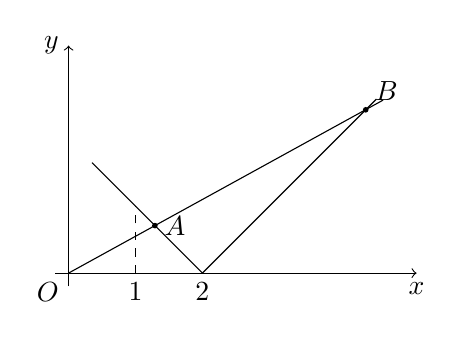
\begin{tikzpicture}[scale=0.85]
\draw[->] (-0.2,0) -- (5.2,0) node[below]{$x$};
\draw[->] (0,-0.2) -- (0,3.4) node[left]{$y$};
\node[below left] at (0,0) {$O$};
\draw (2,0) -- (0.35,1.65);
\draw (2,0) -- (4.6,2.6);
\draw (0,0) -- (4.7,2.585);
\draw[dashed] (1,0) -- (1,1);
\node[below] at (1,0) {$1$};
\node[below] at (2,0) {$2$};
\coordinate (A) at (1.29,0.71); \fill (A) circle (1.2pt); \node[right] at (A) {$A$};
\coordinate (B) at (4.44,2.44); \fill (B) circle (1.2pt); \node[above right] at (B) {$B$};
\end{tikzpicture}
\end{center}
\step{由 $0<k<1$，得 $x_A>1$，}
\step{所以关于 $x$ 的不等式 $k\lvert x\rvert-\lvert x-2\rvert>0$ 恰好有 $4$ 个整数解，是 $2,3,4,5$，}
\step{由 $\begin{cases}y=kx\\ y=x-2\end{cases}\Rightarrow x_B=\dfrac2{1-k}\in(5,6]$，故 $\dfrac35<k\leqslant\dfrac23$.}
\solend
\fi

\item 设集合 $S=\{1,2,3,\cdots,10\}$，$S$ 的子集 $A$ 满足 $A\cap\{1,2,3\}\neq\varnothing$，$A\cup\{4,5,6\}\neq S$，这样的子集 $A$ 的个数为\blankline[4.4em].

\ifanswer
\solbegin
\step{先求使 $A\cap\{1,2,3\}\neq\varnothing$ 成立的 $S$ 的子集 $A$ 的个数 $N_1$，}
\step{在 $\{1,2,3\}$ 中取出至少一个元素的方式有 $7$ 种，}
\step{而集合 $\{4,5,\cdots,10\}$ 的子集有 $2^7$ 个，因此 $N_1=7\times2^7=896$，}
% 注：下一行原卷印作“$A\cup\{4,5,6\}\neq S$”，按上下文应为“$=S$”，照录未改（见文件头“原卷笔误/存疑”①）。
\step{再扣除其中使 $A\cup\{4,5,6\}\neq S$ 的集合 $A$ 的个数 $N_2$，}
\step{这些取法中 $1$，$2$，$3$，$7$，$8$，$9$，$10$ 均被取出，}
\step{而集合 $\{4,5,6\}$ 的子集有 $2^3$ 个，因此 $N_2=2^3=8$，}
\step{从而满足条件的子集 $A$ 的个数为 $N_1-N_2=896-8=888$.}
\solend
\fi

\end{enumerate}

\bigsec{二、选择题}

\begin{enumerate}
\setcounter{enumi}{12}

\item 已知 $a>b$，下列不等式中一定成立是\mbox{（\quad）}

\keepwithprev
A. $a^2>b^2$\qquad B. $ac^2>bc^2$\qquad C. $\dfrac1a<\dfrac1b$\qquad D. $a+3>b-4$

\ifanswer
\solbegin
\step{对于 $A$，当 $a=-2$，$b=-4$ 时，不等式不成立，故 $A$ 错误；}
\step{对于 $B$，当 $c=0$ 时，不等式不成立，故 $B$ 错误；}
\step{对于 $C$，当 $a=2$，$b=-4$ 时，不等式不成立，故 $C$ 错误；}
\step{对于 $D$，因为 $a>b$，$3>-4$，必有 $a+3>b-4$ 成立，故 $D$ 正确.}
\solend
\fi

\item 已知集合 $M$ 满足 $\{2,3\}\subseteq M\subseteq\{1,2,3,4,5\}$，那么这样的集合 $M$ 的个数为\mbox{（\quad）}

\keepwithprev
A. $6$\qquad B. $7$\qquad C. $8$\qquad D. $9$

\ifanswer
\solbegin
\step{集合 $M$ 满足 $\{2,3\}\subseteq M\subseteq\{1,2,3,4,5\}$，所以 $2\in M$，$3\in M$，}
\step{故集合 $M$ 的个数为 $2^3=8$. 故选 $C$.}
\solend
\fi

\item 已知集合 $A=\{x\mid x=2k,k\in\Z\}$，$B=\{x\mid x=4m+6n,m,n\in\Z\}$，则\mbox{（\quad）}

\keepwithprev
A. $B\subset A$\qquad B. $A\subset B$\qquad C. $A=B$\qquad D. $B\neq A$

\ifanswer
\solbegin
\step{$B=\{x\mid x=4m+6n,m,n\in\Z\}$，$B$ 中的元素都是偶数，}
\step{所以 $B$ 的元素都是 $A$ 的元素，$B\subseteq A$；}
\step{$A=\{x\mid x=4(-k)+6k,k\in\Z\}$，则 $A$ 的元素都是 $B$ 的元素，$A\subseteq B$；}
\step{所以 $A=B$. 故选 $C$.}
\solend
\fi

\item 已知集合 $A=[1,a]\cup[a^3,a^4]$，集合 $B=\{x\mid x=x_1-x_2$，其中 $x_1,x_2\in A\}$. 若集合 $B$ 表示的区间为一个闭区间，则 $a$ 的取值范围为\mbox{（\quad）}

\keepwithprev
A. $a$ 取遍任意大于 $1$ 的实数\qquad B. $a\geqslant2$

C. $a\geqslant\dfrac{1+\sqrt5}2$\qquad D. $a\geqslant1+\sqrt2$

\ifanswer
\solbegin
\step{由题意得 $a^3>a>1$，则 $x_1-x_2$ 的最小值为 $1-a^4$，最大值为 $a^4-1$，}
\step{所以 $B=[1-a^4,a^4-1]$，}
\step{又因为 $a^4-a^3-(a-1)=a^3(a-1)-(a-1)=(a^3-1)(a-1)>0$，}
\step{所以 $a^4-a^3>a-1$，又集合 $B$ 表示的区间为一个闭区间，}
\step{则 $a^3-a\leqslant a^4-a^3$，化简得 $a^2-a-1\geqslant0$，又 $a>1$，解得 $a\geqslant\dfrac{1+\sqrt5}2$.}
\step{故选 $C$.}
\solend
\fi

\end{enumerate}

\bigsec{三、解答题}

\begin{enumerate}
\setcounter{enumi}{16}

\item 设全集 $U=\R$，集合 $A=\{x\mid\lvert x+3\rvert\leqslant4\}$，集合 $B=\{x\mid a-2\leqslant x\leqslant1+2a\}$，其中 $a\in\R$.

（1）若 $a=\dfrac12$，求 $A\cap B$；

（2）若 $A\cap B=\varnothing$，求 $a$ 的取值范围.

\ifanswer
\solbegin
\stepm{(1)}{由 $\lvert x+3\rvert\leqslant4$，得 $-4\leqslant x+3\leqslant4$，解得 $-7\leqslant x\leqslant1$，}
\step{所以 $A=\{x\mid-7\leqslant x\leqslant1\}$，}
\step{当 $a=\dfrac12$ 时，$a-2=\dfrac12-2=-\dfrac32$，$1+2a=1+2\times\dfrac12=2$，}
\step{$B=\left\{x\mid-\dfrac32\leqslant x\leqslant2\right\}$，$A\cap B=\left\{x\mid-\dfrac32\leqslant x\leqslant1\right\}$，即 $\left[-\dfrac32,1\right]$.}
\stepm{(2)}{若 $A\cap B=\varnothing$，分两种情况讨论，}
\step{①当 $B\neq\varnothing$ 时，$a-2\leqslant1+2a$，即 $a\geqslant-3$，}
\step{要满足 $A\cap B=\varnothing$，则 $1+2a<-7$ 或 $a-2>1$，}
\step{由 $1+2a<-7$，得 $a<-4$，与 $a\geqslant-3$ 无交集，无解，}
\step{由 $a-2>1$ 得 $a>3$，符合 $a\geqslant-3$，}
\step{②当 $B=\varnothing$ 时，有 $a-2>1+2a$，解得 $a<-3$，满足 $A\cap B=\varnothing$；}
\step{综上，$a$ 的取值范围是 $(-\infty,-3)\cup(3,+\infty)$.}
\solend
\fi

\ansspace

\item （1）已知 $a>b>0$，比较 $\dfrac{a+b}{a^2+b^2}$ 与 $\dfrac1{a-b}$ 的大小并说明理由；

（2）已知 $-2\leqslant x\leqslant-1$，$2\leqslant y\leqslant3$，求 $2x-y$ 的取值范围.

\ifanswer
\solbegin
\stepm{(1)}{$\dfrac{a+b}{a^2+b^2}-\dfrac1{a-b}=\dfrac{(a^2-b^2)-(a^2+b^2)}{(a^2+b^2)(a-b)}=\dfrac{-2b^2}{(a^2+b^2)(a-b)}$，}
\step{因为 $a>b>0$，所以 $a^2(a-b)-b^2(b-a)=(a^2+b^2)(a-b)>0$，}
\step{$\dfrac{-2b^2}{(a^2+b^2)(a-b)}<0$，即 $\dfrac{a+b}{a^2+b^2}-\dfrac1{a-b}<0$，所以 $\dfrac{a+b}{a^2+b^2}<\dfrac1{a-b}$；}
\stepm{(2)}{由 $-2\leqslant x\leqslant-1$，$2\leqslant y\leqslant3$，得 $-4\leqslant2x\leqslant-2$，$-3\leqslant-y\leqslant-2$，}
\step{得 $-7\leqslant2x-y\leqslant-4$，即 $2x-y$ 的取值范围为 $[-7,-4]$.}
\solend
\fi

\ansspace

\item 设 $x_1$、$x_2$ 是关于 $x$ 的方程 $x^2-2(m+2)x+m^2-1=0$ 的两个实数根.

（1）若 $\dfrac1{x_1}+\dfrac1{x_2}=-4$，求 $m$ 的值；

（2）若 $x_1$、$x_2$ 是两个不相等的正数，求实数 $m$ 的取值范围.

\ifanswer
\solbegin
\stepm{(1)}{因为 $x_1$、$x_2$ 是关于 $x$ 的方程的两个实数根，}
\step{所以 $\Delta=(-2(m+2))^2-4(m^2-1)=16m+20\geqslant0$，解得 $m\geqslant-\dfrac54$，}
\step{由韦达定理得 $x_1+x_2=2(m+2)$，$x_1x_2=m^2-1$，}
\step{所以 $\dfrac1{x_1}+\dfrac1{x_2}=\dfrac{x_2+x_1}{x_1x_2}=\dfrac{2(m+2)}{m^2-1}=-4$，即 $2m^2+m=0$，}
\step{解得 $m=0$ 或 $m=-\dfrac12$；}
\stepm{(2)}{由题意得 $\begin{cases}x_1+x_2>0\\ x_1x_2>0\\ \Delta>0\end{cases}$，即 $\begin{cases}2(m+2)>0\\ m^2-1>0\\ (-2(m+2))^2-4(m^2-1)>0\end{cases}$，}
\step{解得 $-\dfrac54<m<-1$ 或 $m>1$.}
\solend
\fi

\ansspace

\ifanswer\else\needvspace{10\baselineskip}\fi
\item 已知集合 $A=\{x\mid x\leqslant2\text{ 或 }x\geqslant a\}$.

（1）若 $B=\left\{x\mid(x-2)\left(x-\dfrac{12}{7-a}\right)<0\right\}$，$A\cap B=\varnothing$，$A\cup B=\R$，求实数 $a$ 的值；

（2）若 $a=3$ 且 $b<2$，$B=\{x\mid x^2-b(b+1)x+b^3<0\}$，$A\cap B\cap\Z$ 的子集个数为 $4$ 个，求实数 $b$ 的取值范围.

\ifanswer
\solbegin
\stepm{(1)}{当 $a\leqslant2$ 时，$A=\{x\mid x\leqslant2\text{ 或 }x\geqslant a\}=\R$，必有 $B=\varnothing$，}
\step{即不等式 $(x-2)\left(x-\dfrac{12}{7-a}\right)<0$ 无解，}
\step{必有 $\dfrac{12}{7-a}=2$，解得 $a=1$，符合题意，}
\step{当 $a>2$ 时，$A=(-\infty,2]\cup[a,+\infty)$，}
\step{若 $A\cap B=\varnothing$，$A\cup B=\R$，则 $B=(2,a)$，}
\step{即方程 $(x-2)\left(x-\dfrac{12}{7-a}\right)=0$ 的两个根是 $2$ 和 $a$，所以 $\dfrac{12}{7-a}=a$，}
\step{解得 $a=3$ 或 $a=4$，符合题意，}
\step{综上，实数 $a$ 的值为 $1$ 或 $3$ 或 $4$；}
\stepm{(2)}{由 $A\cap B\cap\Z$ 的子集个数为 $4$ 个，即 $A\cap B\cap\Z$ 中恰好有 $2$ 个整数元素，}
\step{由 $a=3$，则 $A=(-\infty,2]\cup[3,+\infty)$，}
\step{由 $x^2-b(b+1)x+b^3=(x-b^2)(x-b)<0$，又 $b<2$，}
\step{当 $1<b<2$ 时，$1<b^2<4$ 且 $b^2>b$，则 $B=(b,b^2)$，}
\step{则 $A\cap B=(b,2]\cup[3,b^2)$，}
\step{要使 $A\cap B\cap\Z$ 中恰好有 $2$ 个整数元素，即 $A\cap B\cap\Z=\{2,3\}$，}
\step{即 $\begin{cases}1<b<2\\ 3<b^2<4\end{cases}$，解得 $\sqrt3<b<2$，符合题意，}
\step{当 $b=1$ 或 $b=0$ 时，$B=\varnothing$，此时 $A\cap B\cap\Z=\varnothing$，不符合题意，舍去，}
\step{当 $0<b<1$ 时，$0<b^2<1$ 且 $b^2<b$，则 $B=(b^2,b)$，}
\step{此时 $A\cap B\cap\Z=\varnothing$，不符合题意，舍去，}
\step{当 $-1<b<0$ 时，$0<b^2<1$ 且 $b^2>b$，则 $B=(b,b^2)$，}
\step{此时 $A\cap B\cap\Z=\{0\}$，即 $A\cap B\cap\Z$ 中只有 $1$ 个元素，不符合题意，舍去，}
\step{当 $b\leqslant-1$ 时，$b^2\geqslant1$ 且 $b^2>b$，则 $B=(b,b^2)$，}
\step{此时 $A\cap B\cap\Z\supseteq\{-1,0,1\}$，即 $A\cap B\cap\Z$ 中至少有 $3$ 个元素，}
\step{不符合题意，舍去，}
\step{综上，实数 $b$ 的取值范围为 $(\sqrt3,2)$.}
\solend
\fi

\ansspace*[7]

\item 已知集合 $A=\{a_1,a_2,a_3,\cdots,a_n\}$ 中的元素均为正整数，其中 $n\in\N$ 且 $n\geqslant3$. 若对任意 $x,y\in A(x\neq y)$，都有 $\lvert x-y\rvert\geqslant\dfrac{xy}k$，则称集合 $A$ 具有性质 $M_k$.

（1）集合 $A=\{1,2,a\}$ 具有性质 $M_3$，求 $a$ 的最小值；

（2）若集合 $A$ 具有性质 $M_{24}$，且 $A$ 中最小元素和最大元素分别为 $a,b$，求证：$\dfrac1a-\dfrac1b\geqslant\dfrac{n-1}{24}$；

（3）已知集合 $A$ 具有性质 $M_{24}$，求 $A$ 中元素个数的最大值，并说明理由.

\ifanswer
\solbegin
\stepm{(1)}{由性质 $M_3$ 定义得 $\begin{cases}a-1\geqslant\dfrac a3\\ a-2\geqslant\dfrac{2a}3\end{cases}\Rightarrow\begin{cases}a\geqslant\dfrac32\\ a\geqslant6\end{cases}\Rightarrow a\geqslant6$，且 $a\subseteq\N^*$，}
% 注：上一行原卷印作“$a\subseteq\N^*$”，应为“$a\in\N^*$”，照录未改（见文件头“原卷笔误/存疑”②）。
\step{所以 $a$ 的最小值为 $6$.}
\stepm{(2)}{由题意得 $\lvert a_i-a_{i+1}\rvert\geqslant\dfrac{a_ia_{i+1}}{24}$，$(i=1,2,3,\cdots,n-1)$，且 $a_1<\cdots<a_n$，}
\step{所以 $a_{i+1}-a_i\geqslant\dfrac{a_ia_{i+1}}{24}\Rightarrow\dfrac1{a_i}-\dfrac1{a_{i+1}}\geqslant\dfrac1{24}$，$(i=1,2,3,\cdots,n-1)$，}
\step{所以 $\dfrac1{a_1}-\dfrac1{a_2}+\dfrac1{a_2}-\dfrac1{a_3}+\cdots+\dfrac1{a_{n-1}}-\dfrac1{a_n}=\dfrac1{a_1}-\dfrac1{a_n}\geqslant\dfrac{n-1}{24}$，得证.}
\stepm{(3)}{由 (2) 得 $\begin{cases}\dfrac1{a_1}\geqslant\dfrac{n-1}{24}\\ a_1\geqslant1\end{cases}\Rightarrow\dfrac{n-1}{24}<1\Rightarrow n<25$，}
\step{同 (2) 证明得 $\dfrac1{a_i}-\dfrac1{a_n}\geqslant\dfrac{n-i}{24}$ 且 $i=1,2,3,\cdots,n-1$，故 $\dfrac1{a_i}>\dfrac{n-i}{24}$，}
\step{又 $a_i\geqslant i$，所以 $\dfrac1i>\dfrac{n-i}{24}\Rightarrow i(n-i)<24$ 在 $i=1,2,3,\cdots,n-1$ 上恒成立，}
\step{当 $n\geqslant10$，取 $i=5$，则 $i(n-i)=5(n-5)>24$，故 $n<10$，}
\step{当 $n\leqslant9$，则 $i(n-i)\leqslant\dfrac{(i+n-i)^2}4=\dfrac{n^2}4<24\Rightarrow n<\sqrt{96}$，即 $n\leqslant9$.}
\step{综上，集合 $A$ 中元素个数的最大值为 $9$.}
\solend
\fi

\end{enumerate}

\end{document}
"
%
% 原始材料：微信公众号“魔都数学加油站”文章，连载“27学年高一79”；
% 原文标题“27学年高一79——2026-2027年上海市南汇中学高一上10月月考”；
% 原文链接：https://mp.weixin.qq.com/s/bFvc7GVgPTaDGg_6JSSfGg。
% 页面标注发布时间 2026-10-24 21:00（上海）。
% 正文为 9 张 PNG 页（`原图/高一79_南汇中学_10月月考/01..09.png`），
% 尺寸混排（第 1、2、4、5、7、8 页为 4762×6735，第 3、6、9 页为 2560×3620），均按页序读取。
%
% 篇幅与题号：原卷自第 3 题起编号。填空题 3—12（10 题）、选择题 13—16（4 题）、
% 解答题 17—21（5 题），共 19 题。
%
% 讲评版：第 4 题只印【答案】，本稿只给 \ans{}；其余 18 题印【解析】。
% 选择题答案在解析末句“故选 D／C／C／C”。
%
% 副标题：原卷未印副标题。本稿按内容标作“集合与常用逻辑用语、不等式”。
%
% 原卷笔误/存疑（均照录未改，正文对应处另有 % 注）：
%   ① 第 12 题解析作“再扣除其中使 $A\cup\{4,5,6\}\neq S$ 的集合 $A$ 的个数 $N_2$”，
%      按上下文应为“$A\cup\{4,5,6\}=S$”，否则“这些取法中 $1,2,3,7,8,9,10$ 均被取出”
%      与 $N_2=2^3=8$ 都无法解释；原卷印作 $\neq$，照录未改。
%   ② 第 21 题 (1) 解析末作“且 $a\subseteq\N^*$”，$a$ 是集合的元素，应为 $a\in\N^*$；
%      原卷印作 $\subseteq$，照录未改。
%
% 与原卷的排版差异：
%   ① 原卷每题下直接印【答案】/【解析】，本稿按全稿惯例将答案与解析置于答案版；
%   ② 原卷未印副标题，本稿补出；填空横线统一排 \blankline[4.4em]；
%   ③ 原卷数集记号排斜体 $R$、$Z$、$N$，本稿按全稿惯例改用 $\R$、$\Z$、$\N$；
%   ④ 第 17—21 题的子问用行内“（1）（2）（3）”段，解析中的子问标号用 \stepm；
%   ⑤ 解答题按惯例加 \ansspace；选择题括号排 \mbox{（\quad）}；
%   ⑥ 第 11 题解析有一幅函数图象（$y=k\lvert x\rvert$ 与 $y=\lvert x-2\rvert$），
%      按原图形状用 TikZ 重排（仅答案版出）。
%
% 行数核对：逐题数 \step/\stepm 条数，合计 107 条（Q3：2；Q5：2；Q6：1；Q7：4；Q8：4；
% Q9：4；Q10：5；Q11：4；Q12：7；Q13：4；Q14：2；Q15：4；Q16：6；Q17：11；Q18：5；
% Q19：7；Q20：24；Q21：11）。原卷解析的换行按语意合并，未逐行强拆；第 4 题只印
% 【答案】，提 \ans{}，不计入 \step 账。
%
\documentclass[a4paper,11pt]{article}
\usepackage{common}

\begin{document}

\examtitlest[3]{2026--2027 年南汇中学高一上 10 月月考}{集合与常用逻辑用语、不等式}

\bigsec{一、填空题}

\begin{enumerate}
\setcounter{enumi}{2}

\item 不等式 $\dfrac{1-x}{x}>0$ 的解集为\blankline[4.4em].

\ifanswer
\solbegin
\step{原不等式化为 $x(x-1)<0$，转化为 $\begin{cases}x>0\\ x-1<0\end{cases}$ 或 $\begin{cases}x<0\\ x-1>0\end{cases}$，}
\step{解得 $0<x<1$，则不等式的解集为 $\{x\mid0<x<1\}$.}
\solend
\fi

\item 用反证法证明命题：“若 $x^2<1$，则 $-1<x<1$”时，应假设\blankline[4.4em].

\ifanswer
\ans{$x\geqslant1$ 或 $x\leqslant-1$}
\fi

\item 设 $k$ 为实数，关于 $x$ 的不等式 $kx^2+x+2<0$ 的解集为 $A$，若 $2\notin A$，则 $k$ 的取值范围是\blankline[4.4em].

\ifanswer
\solbegin
\step{因为关于 $x$ 的不等式 $kx^2+x+2<0$ 的解集为 $A$，且 $2\notin A$，}
\step{所以 $x=2$ 时，$k\times2^2+2+2\geqslant0$，解得 $k\geqslant-1$，则 $k$ 的取值范围为 $[-1,+\infty)$.}
\solend
\fi

\item 已知集合 $M=\{y\mid y=x^2-2x,x\in\R\}$，$N=\{x\mid y=\sqrt{4-x^2}\}$，则 $M\cup N=$\blankline[4.4em].

\ifanswer
\solbegin
\step{$M=[-1,+\infty)$，$N=[-2,2]$，则 $M\cup N=[-2,+\infty)$.}
\solend
\fi

\item 设集合 $A=\{-3,2\}$，集合 $B=\{x\mid mx+1=0\}$，且 $A\cup B=A$，则 $m$ 的值组成的集合是\blankline[4.4em].

\ifanswer
\solbegin
\step{由 $A\cup B=A$，得 $B\subseteq A$，}
\step{当 $m=0$ 时，$B=\varnothing$，满足题意，}
\step{当 $m\neq0$ 时，$B=\left\{-\dfrac1m\right\}$，所以 $-\dfrac1m=2$ 或 $-\dfrac1m=-3$，所以 $m=-\dfrac12$ 或 $m=\dfrac13$，}
\step{综上所述，$m$ 的值组成的集合是 $\left\{0,-\dfrac12,\dfrac13\right\}$.}
\solend
\fi

\item 若不等式 $\lvert x\rvert<a$ 的一个充分不必要条件为 $\dfrac{2x-1}{x-2}<1$，则实数 $a$ 的取值范围是\blankline[4.4em].

\ifanswer
\solbegin
\step{不等式 $\lvert x\rvert<a$，得 $-a<x<a$，}
\step{不等式 $\dfrac{2x-1}{x-2}<1$，即 $\dfrac{2x-1-(x-2)}{x-2}=\dfrac{x+1}{x-2}<0$，解得 $-1<x<2$，}
\step{又不等式 $\lvert x\rvert<a$ 的一个充分不必要条件为 $\dfrac{2x-1}{x-2}<1$，}
\step{得 $\begin{cases}a\geqslant2\\ -a\leqslant-1\end{cases}$，且两等号不同时成立，解得 $a\geqslant2$.}
\solend
\fi

\item 若对任意 $x\in\R$ 都有 $(m-1)x^2-(m-1)x-1<0$，则实数 $m$ 的取值范围是\blankline[4.4em].

\ifanswer
\solbegin
\step{当 $m-1\neq0$，即 $m\neq1$ 时，则有 $\begin{cases}m-1<0\\ (m-1)^2-4(m-1)\times(-1)<0\end{cases}$，}
\step{解得 $-3<m<1$；}
\step{当 $m-1=0$ 时，即当 $m=1$ 时，此时不等式为 $-1<0$ 恒成立，符合题意；}
\step{综上所述，实数 $m$ 的取值范围是 $(-3,1]$.}
\solend
\fi

\item 关于 $x$ 的方程 $\dfrac{x}{x-1}=\dfrac{k-x}{x^2-x}$ 的解集中只含有一个元素，则 $k$ 的可能取值构成的集合为\blankline[4.4em].

\ifanswer
\solbegin
\step{方程两边同时乘以 $x(x-1)$ 得 $x^2=k-x$，即 $x^2+x-k=0$，}
\step{①当其中一个解为增根时，方程也只有一个解，}
\step{(i) 若增根为 $0$ 时，$k=0$；(ii) 若增根为 $1$ 时，$k=2$；}
\step{②当 $\Delta=1+4k=0$，即 $k=-\dfrac14$ 时，方程 $x^2+x-k=0$ 只有一个解；}
\step{即 $k$ 的可能取值构成的集合为 $\left\{-\dfrac14,0,2\right\}$.}
\solend
\fi

\item 若关于 $x$ 的不等式 $k\lvert x\rvert>\lvert x-2\rvert$ 恰好有 $4$ 个整数解，则实数 $k$ 的取值范围是\blankline[4.4em].

\ifanswer
\solbegin
\step{由题意得 $0<k<1$，函数 $y=k\lvert x\rvert$ 与 $y=\lvert x-2\rvert$ 的图象如图：}
\begin{center}
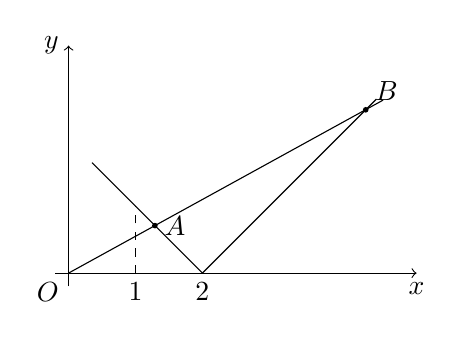
\begin{tikzpicture}[scale=0.85]
\draw[->] (-0.2,0) -- (5.2,0) node[below]{$x$};
\draw[->] (0,-0.2) -- (0,3.4) node[left]{$y$};
\node[below left] at (0,0) {$O$};
\draw (2,0) -- (0.35,1.65);
\draw (2,0) -- (4.6,2.6);
\draw (0,0) -- (4.7,2.585);
\draw[dashed] (1,0) -- (1,1);
\node[below] at (1,0) {$1$};
\node[below] at (2,0) {$2$};
\coordinate (A) at (1.29,0.71); \fill (A) circle (1.2pt); \node[right] at (A) {$A$};
\coordinate (B) at (4.44,2.44); \fill (B) circle (1.2pt); \node[above right] at (B) {$B$};
\end{tikzpicture}
\end{center}
\step{由 $0<k<1$，得 $x_A>1$，}
\step{所以关于 $x$ 的不等式 $k\lvert x\rvert-\lvert x-2\rvert>0$ 恰好有 $4$ 个整数解，是 $2,3,4,5$，}
\step{由 $\begin{cases}y=kx\\ y=x-2\end{cases}\Rightarrow x_B=\dfrac2{1-k}\in(5,6]$，故 $\dfrac35<k\leqslant\dfrac23$.}
\solend
\fi

\item 设集合 $S=\{1,2,3,\cdots,10\}$，$S$ 的子集 $A$ 满足 $A\cap\{1,2,3\}\neq\varnothing$，$A\cup\{4,5,6\}\neq S$，这样的子集 $A$ 的个数为\blankline[4.4em].

\ifanswer
\solbegin
\step{先求使 $A\cap\{1,2,3\}\neq\varnothing$ 成立的 $S$ 的子集 $A$ 的个数 $N_1$，}
\step{在 $\{1,2,3\}$ 中取出至少一个元素的方式有 $7$ 种，}
\step{而集合 $\{4,5,\cdots,10\}$ 的子集有 $2^7$ 个，因此 $N_1=7\times2^7=896$，}
% 注：下一行原卷印作“$A\cup\{4,5,6\}\neq S$”，按上下文应为“$=S$”，照录未改（见文件头“原卷笔误/存疑”①）。
\step{再扣除其中使 $A\cup\{4,5,6\}\neq S$ 的集合 $A$ 的个数 $N_2$，}
\step{这些取法中 $1$，$2$，$3$，$7$，$8$，$9$，$10$ 均被取出，}
\step{而集合 $\{4,5,6\}$ 的子集有 $2^3$ 个，因此 $N_2=2^3=8$，}
\step{从而满足条件的子集 $A$ 的个数为 $N_1-N_2=896-8=888$.}
\solend
\fi

\end{enumerate}

\bigsec{二、选择题}

\begin{enumerate}
\setcounter{enumi}{12}

\item 已知 $a>b$，下列不等式中一定成立是\mbox{（\quad）}

\keepwithprev
A. $a^2>b^2$\qquad B. $ac^2>bc^2$\qquad C. $\dfrac1a<\dfrac1b$\qquad D. $a+3>b-4$

\ifanswer
\solbegin
\step{对于 $A$，当 $a=-2$，$b=-4$ 时，不等式不成立，故 $A$ 错误；}
\step{对于 $B$，当 $c=0$ 时，不等式不成立，故 $B$ 错误；}
\step{对于 $C$，当 $a=2$，$b=-4$ 时，不等式不成立，故 $C$ 错误；}
\step{对于 $D$，因为 $a>b$，$3>-4$，必有 $a+3>b-4$ 成立，故 $D$ 正确.}
\solend
\fi

\item 已知集合 $M$ 满足 $\{2,3\}\subseteq M\subseteq\{1,2,3,4,5\}$，那么这样的集合 $M$ 的个数为\mbox{（\quad）}

\keepwithprev
A. $6$\qquad B. $7$\qquad C. $8$\qquad D. $9$

\ifanswer
\solbegin
\step{集合 $M$ 满足 $\{2,3\}\subseteq M\subseteq\{1,2,3,4,5\}$，所以 $2\in M$，$3\in M$，}
\step{故集合 $M$ 的个数为 $2^3=8$. 故选 $C$.}
\solend
\fi

\item 已知集合 $A=\{x\mid x=2k,k\in\Z\}$，$B=\{x\mid x=4m+6n,m,n\in\Z\}$，则\mbox{（\quad）}

\keepwithprev
A. $B\subset A$\qquad B. $A\subset B$\qquad C. $A=B$\qquad D. $B\neq A$

\ifanswer
\solbegin
\step{$B=\{x\mid x=4m+6n,m,n\in\Z\}$，$B$ 中的元素都是偶数，}
\step{所以 $B$ 的元素都是 $A$ 的元素，$B\subseteq A$；}
\step{$A=\{x\mid x=4(-k)+6k,k\in\Z\}$，则 $A$ 的元素都是 $B$ 的元素，$A\subseteq B$；}
\step{所以 $A=B$. 故选 $C$.}
\solend
\fi

\item 已知集合 $A=[1,a]\cup[a^3,a^4]$，集合 $B=\{x\mid x=x_1-x_2$，其中 $x_1,x_2\in A\}$. 若集合 $B$ 表示的区间为一个闭区间，则 $a$ 的取值范围为\mbox{（\quad）}

\keepwithprev
A. $a$ 取遍任意大于 $1$ 的实数\qquad B. $a\geqslant2$

C. $a\geqslant\dfrac{1+\sqrt5}2$\qquad D. $a\geqslant1+\sqrt2$

\ifanswer
\solbegin
\step{由题意得 $a^3>a>1$，则 $x_1-x_2$ 的最小值为 $1-a^4$，最大值为 $a^4-1$，}
\step{所以 $B=[1-a^4,a^4-1]$，}
\step{又因为 $a^4-a^3-(a-1)=a^3(a-1)-(a-1)=(a^3-1)(a-1)>0$，}
\step{所以 $a^4-a^3>a-1$，又集合 $B$ 表示的区间为一个闭区间，}
\step{则 $a^3-a\leqslant a^4-a^3$，化简得 $a^2-a-1\geqslant0$，又 $a>1$，解得 $a\geqslant\dfrac{1+\sqrt5}2$.}
\step{故选 $C$.}
\solend
\fi

\end{enumerate}

\bigsec{三、解答题}

\begin{enumerate}
\setcounter{enumi}{16}

\item 设全集 $U=\R$，集合 $A=\{x\mid\lvert x+3\rvert\leqslant4\}$，集合 $B=\{x\mid a-2\leqslant x\leqslant1+2a\}$，其中 $a\in\R$.

（1）若 $a=\dfrac12$，求 $A\cap B$；

（2）若 $A\cap B=\varnothing$，求 $a$ 的取值范围.

\ifanswer
\solbegin
\stepm{(1)}{由 $\lvert x+3\rvert\leqslant4$，得 $-4\leqslant x+3\leqslant4$，解得 $-7\leqslant x\leqslant1$，}
\step{所以 $A=\{x\mid-7\leqslant x\leqslant1\}$，}
\step{当 $a=\dfrac12$ 时，$a-2=\dfrac12-2=-\dfrac32$，$1+2a=1+2\times\dfrac12=2$，}
\step{$B=\left\{x\mid-\dfrac32\leqslant x\leqslant2\right\}$，$A\cap B=\left\{x\mid-\dfrac32\leqslant x\leqslant1\right\}$，即 $\left[-\dfrac32,1\right]$.}
\stepm{(2)}{若 $A\cap B=\varnothing$，分两种情况讨论，}
\step{①当 $B\neq\varnothing$ 时，$a-2\leqslant1+2a$，即 $a\geqslant-3$，}
\step{要满足 $A\cap B=\varnothing$，则 $1+2a<-7$ 或 $a-2>1$，}
\step{由 $1+2a<-7$，得 $a<-4$，与 $a\geqslant-3$ 无交集，无解，}
\step{由 $a-2>1$ 得 $a>3$，符合 $a\geqslant-3$，}
\step{②当 $B=\varnothing$ 时，有 $a-2>1+2a$，解得 $a<-3$，满足 $A\cap B=\varnothing$；}
\step{综上，$a$ 的取值范围是 $(-\infty,-3)\cup(3,+\infty)$.}
\solend
\fi

\ansspace

\item （1）已知 $a>b>0$，比较 $\dfrac{a+b}{a^2+b^2}$ 与 $\dfrac1{a-b}$ 的大小并说明理由；

（2）已知 $-2\leqslant x\leqslant-1$，$2\leqslant y\leqslant3$，求 $2x-y$ 的取值范围.

\ifanswer
\solbegin
\stepm{(1)}{$\dfrac{a+b}{a^2+b^2}-\dfrac1{a-b}=\dfrac{(a^2-b^2)-(a^2+b^2)}{(a^2+b^2)(a-b)}=\dfrac{-2b^2}{(a^2+b^2)(a-b)}$，}
\step{因为 $a>b>0$，所以 $a^2(a-b)-b^2(b-a)=(a^2+b^2)(a-b)>0$，}
\step{$\dfrac{-2b^2}{(a^2+b^2)(a-b)}<0$，即 $\dfrac{a+b}{a^2+b^2}-\dfrac1{a-b}<0$，所以 $\dfrac{a+b}{a^2+b^2}<\dfrac1{a-b}$；}
\stepm{(2)}{由 $-2\leqslant x\leqslant-1$，$2\leqslant y\leqslant3$，得 $-4\leqslant2x\leqslant-2$，$-3\leqslant-y\leqslant-2$，}
\step{得 $-7\leqslant2x-y\leqslant-4$，即 $2x-y$ 的取值范围为 $[-7,-4]$.}
\solend
\fi

\ansspace

\item 设 $x_1$、$x_2$ 是关于 $x$ 的方程 $x^2-2(m+2)x+m^2-1=0$ 的两个实数根.

（1）若 $\dfrac1{x_1}+\dfrac1{x_2}=-4$，求 $m$ 的值；

（2）若 $x_1$、$x_2$ 是两个不相等的正数，求实数 $m$ 的取值范围.

\ifanswer
\solbegin
\stepm{(1)}{因为 $x_1$、$x_2$ 是关于 $x$ 的方程的两个实数根，}
\step{所以 $\Delta=(-2(m+2))^2-4(m^2-1)=16m+20\geqslant0$，解得 $m\geqslant-\dfrac54$，}
\step{由韦达定理得 $x_1+x_2=2(m+2)$，$x_1x_2=m^2-1$，}
\step{所以 $\dfrac1{x_1}+\dfrac1{x_2}=\dfrac{x_2+x_1}{x_1x_2}=\dfrac{2(m+2)}{m^2-1}=-4$，即 $2m^2+m=0$，}
\step{解得 $m=0$ 或 $m=-\dfrac12$；}
\stepm{(2)}{由题意得 $\begin{cases}x_1+x_2>0\\ x_1x_2>0\\ \Delta>0\end{cases}$，即 $\begin{cases}2(m+2)>0\\ m^2-1>0\\ (-2(m+2))^2-4(m^2-1)>0\end{cases}$，}
\step{解得 $-\dfrac54<m<-1$ 或 $m>1$.}
\solend
\fi

\ansspace

\ifanswer\else\needvspace{10\baselineskip}\fi
\item 已知集合 $A=\{x\mid x\leqslant2\text{ 或 }x\geqslant a\}$.

（1）若 $B=\left\{x\mid(x-2)\left(x-\dfrac{12}{7-a}\right)<0\right\}$，$A\cap B=\varnothing$，$A\cup B=\R$，求实数 $a$ 的值；

（2）若 $a=3$ 且 $b<2$，$B=\{x\mid x^2-b(b+1)x+b^3<0\}$，$A\cap B\cap\Z$ 的子集个数为 $4$ 个，求实数 $b$ 的取值范围.

\ifanswer
\solbegin
\stepm{(1)}{当 $a\leqslant2$ 时，$A=\{x\mid x\leqslant2\text{ 或 }x\geqslant a\}=\R$，必有 $B=\varnothing$，}
\step{即不等式 $(x-2)\left(x-\dfrac{12}{7-a}\right)<0$ 无解，}
\step{必有 $\dfrac{12}{7-a}=2$，解得 $a=1$，符合题意，}
\step{当 $a>2$ 时，$A=(-\infty,2]\cup[a,+\infty)$，}
\step{若 $A\cap B=\varnothing$，$A\cup B=\R$，则 $B=(2,a)$，}
\step{即方程 $(x-2)\left(x-\dfrac{12}{7-a}\right)=0$ 的两个根是 $2$ 和 $a$，所以 $\dfrac{12}{7-a}=a$，}
\step{解得 $a=3$ 或 $a=4$，符合题意，}
\step{综上，实数 $a$ 的值为 $1$ 或 $3$ 或 $4$；}
\stepm{(2)}{由 $A\cap B\cap\Z$ 的子集个数为 $4$ 个，即 $A\cap B\cap\Z$ 中恰好有 $2$ 个整数元素，}
\step{由 $a=3$，则 $A=(-\infty,2]\cup[3,+\infty)$，}
\step{由 $x^2-b(b+1)x+b^3=(x-b^2)(x-b)<0$，又 $b<2$，}
\step{当 $1<b<2$ 时，$1<b^2<4$ 且 $b^2>b$，则 $B=(b,b^2)$，}
\step{则 $A\cap B=(b,2]\cup[3,b^2)$，}
\step{要使 $A\cap B\cap\Z$ 中恰好有 $2$ 个整数元素，即 $A\cap B\cap\Z=\{2,3\}$，}
\step{即 $\begin{cases}1<b<2\\ 3<b^2<4\end{cases}$，解得 $\sqrt3<b<2$，符合题意，}
\step{当 $b=1$ 或 $b=0$ 时，$B=\varnothing$，此时 $A\cap B\cap\Z=\varnothing$，不符合题意，舍去，}
\step{当 $0<b<1$ 时，$0<b^2<1$ 且 $b^2<b$，则 $B=(b^2,b)$，}
\step{此时 $A\cap B\cap\Z=\varnothing$，不符合题意，舍去，}
\step{当 $-1<b<0$ 时，$0<b^2<1$ 且 $b^2>b$，则 $B=(b,b^2)$，}
\step{此时 $A\cap B\cap\Z=\{0\}$，即 $A\cap B\cap\Z$ 中只有 $1$ 个元素，不符合题意，舍去，}
\step{当 $b\leqslant-1$ 时，$b^2\geqslant1$ 且 $b^2>b$，则 $B=(b,b^2)$，}
\step{此时 $A\cap B\cap\Z\supseteq\{-1,0,1\}$，即 $A\cap B\cap\Z$ 中至少有 $3$ 个元素，}
\step{不符合题意，舍去，}
\step{综上，实数 $b$ 的取值范围为 $(\sqrt3,2)$.}
\solend
\fi

\ansspace*[7]

\item 已知集合 $A=\{a_1,a_2,a_3,\cdots,a_n\}$ 中的元素均为正整数，其中 $n\in\N$ 且 $n\geqslant3$. 若对任意 $x,y\in A(x\neq y)$，都有 $\lvert x-y\rvert\geqslant\dfrac{xy}k$，则称集合 $A$ 具有性质 $M_k$.

（1）集合 $A=\{1,2,a\}$ 具有性质 $M_3$，求 $a$ 的最小值；

（2）若集合 $A$ 具有性质 $M_{24}$，且 $A$ 中最小元素和最大元素分别为 $a,b$，求证：$\dfrac1a-\dfrac1b\geqslant\dfrac{n-1}{24}$；

（3）已知集合 $A$ 具有性质 $M_{24}$，求 $A$ 中元素个数的最大值，并说明理由.

\ifanswer
\solbegin
\stepm{(1)}{由性质 $M_3$ 定义得 $\begin{cases}a-1\geqslant\dfrac a3\\ a-2\geqslant\dfrac{2a}3\end{cases}\Rightarrow\begin{cases}a\geqslant\dfrac32\\ a\geqslant6\end{cases}\Rightarrow a\geqslant6$，且 $a\subseteq\N^*$，}
% 注：上一行原卷印作“$a\subseteq\N^*$”，应为“$a\in\N^*$”，照录未改（见文件头“原卷笔误/存疑”②）。
\step{所以 $a$ 的最小值为 $6$.}
\stepm{(2)}{由题意得 $\lvert a_i-a_{i+1}\rvert\geqslant\dfrac{a_ia_{i+1}}{24}$，$(i=1,2,3,\cdots,n-1)$，且 $a_1<\cdots<a_n$，}
\step{所以 $a_{i+1}-a_i\geqslant\dfrac{a_ia_{i+1}}{24}\Rightarrow\dfrac1{a_i}-\dfrac1{a_{i+1}}\geqslant\dfrac1{24}$，$(i=1,2,3,\cdots,n-1)$，}
\step{所以 $\dfrac1{a_1}-\dfrac1{a_2}+\dfrac1{a_2}-\dfrac1{a_3}+\cdots+\dfrac1{a_{n-1}}-\dfrac1{a_n}=\dfrac1{a_1}-\dfrac1{a_n}\geqslant\dfrac{n-1}{24}$，得证.}
\stepm{(3)}{由 (2) 得 $\begin{cases}\dfrac1{a_1}\geqslant\dfrac{n-1}{24}\\ a_1\geqslant1\end{cases}\Rightarrow\dfrac{n-1}{24}<1\Rightarrow n<25$，}
\step{同 (2) 证明得 $\dfrac1{a_i}-\dfrac1{a_n}\geqslant\dfrac{n-i}{24}$ 且 $i=1,2,3,\cdots,n-1$，故 $\dfrac1{a_i}>\dfrac{n-i}{24}$，}
\step{又 $a_i\geqslant i$，所以 $\dfrac1i>\dfrac{n-i}{24}\Rightarrow i(n-i)<24$ 在 $i=1,2,3,\cdots,n-1$ 上恒成立，}
\step{当 $n\geqslant10$，取 $i=5$，则 $i(n-i)=5(n-5)>24$，故 $n<10$，}
\step{当 $n\leqslant9$，则 $i(n-i)\leqslant\dfrac{(i+n-i)^2}4=\dfrac{n^2}4<24\Rightarrow n<\sqrt{96}$，即 $n\leqslant9$.}
\step{综上，集合 $A$ 中元素个数的最大值为 $9$.}
\solend
\fi

\end{enumerate}

\end{document}
"
% 紧凑版：xelatex "\def\iscompact{1}% 高一79_南汇中学_10月月考.tex
%   —— 高一上数学“2026-2027 年南汇中学高一上 10 月月考”（讲评版）
% 试卷版：xelatex 高一79_南汇中学_10月月考.tex
% 答案版：xelatex "\def\isanswer{1}% 高一79_南汇中学_10月月考.tex
%   —— 高一上数学“2026-2027 年南汇中学高一上 10 月月考”（讲评版）
% 试卷版：xelatex 高一79_南汇中学_10月月考.tex
% 答案版：xelatex "\def\isanswer{1}% 高一79_南汇中学_10月月考.tex
%   —— 高一上数学“2026-2027 年南汇中学高一上 10 月月考”（讲评版）
% 试卷版：xelatex 高一79_南汇中学_10月月考.tex
% 答案版：xelatex "\def\isanswer{1}\input{高一79_南汇中学_10月月考.tex}"
% 紧凑版：xelatex "\def\iscompact{1}\input{高一79_南汇中学_10月月考.tex}"
%
% 原始材料：微信公众号“魔都数学加油站”文章，连载“27学年高一79”；
% 原文标题“27学年高一79——2026-2027年上海市南汇中学高一上10月月考”；
% 原文链接：https://mp.weixin.qq.com/s/bFvc7GVgPTaDGg_6JSSfGg。
% 页面标注发布时间 2026-10-24 21:00（上海）。
% 正文为 9 张 PNG 页（`原图/高一79_南汇中学_10月月考/01..09.png`），
% 尺寸混排（第 1、2、4、5、7、8 页为 4762×6735，第 3、6、9 页为 2560×3620），均按页序读取。
%
% 篇幅与题号：原卷自第 3 题起编号。填空题 3—12（10 题）、选择题 13—16（4 题）、
% 解答题 17—21（5 题），共 19 题。
%
% 讲评版：第 4 题只印【答案】，本稿只给 \ans{}；其余 18 题印【解析】。
% 选择题答案在解析末句“故选 D／C／C／C”。
%
% 副标题：原卷未印副标题。本稿按内容标作“集合与常用逻辑用语、不等式”。
%
% 原卷笔误/存疑（均照录未改，正文对应处另有 % 注）：
%   ① 第 12 题解析作“再扣除其中使 $A\cup\{4,5,6\}\neq S$ 的集合 $A$ 的个数 $N_2$”，
%      按上下文应为“$A\cup\{4,5,6\}=S$”，否则“这些取法中 $1,2,3,7,8,9,10$ 均被取出”
%      与 $N_2=2^3=8$ 都无法解释；原卷印作 $\neq$，照录未改。
%   ② 第 21 题 (1) 解析末作“且 $a\subseteq\N^*$”，$a$ 是集合的元素，应为 $a\in\N^*$；
%      原卷印作 $\subseteq$，照录未改。
%
% 与原卷的排版差异：
%   ① 原卷每题下直接印【答案】/【解析】，本稿按全稿惯例将答案与解析置于答案版；
%   ② 原卷未印副标题，本稿补出；填空横线统一排 \blankline[4.4em]；
%   ③ 原卷数集记号排斜体 $R$、$Z$、$N$，本稿按全稿惯例改用 $\R$、$\Z$、$\N$；
%   ④ 第 17—21 题的子问用行内“（1）（2）（3）”段，解析中的子问标号用 \stepm；
%   ⑤ 解答题按惯例加 \ansspace；选择题括号排 \mbox{（\quad）}；
%   ⑥ 第 11 题解析有一幅函数图象（$y=k\lvert x\rvert$ 与 $y=\lvert x-2\rvert$），
%      按原图形状用 TikZ 重排（仅答案版出）。
%
% 行数核对：逐题数 \step/\stepm 条数，合计 107 条（Q3：2；Q5：2；Q6：1；Q7：4；Q8：4；
% Q9：4；Q10：5；Q11：4；Q12：7；Q13：4；Q14：2；Q15：4；Q16：6；Q17：11；Q18：5；
% Q19：7；Q20：24；Q21：11）。原卷解析的换行按语意合并，未逐行强拆；第 4 题只印
% 【答案】，提 \ans{}，不计入 \step 账。
%
\documentclass[a4paper,11pt]{article}
\usepackage{common}

\begin{document}

\examtitlest[3]{2026--2027 年南汇中学高一上 10 月月考}{集合与常用逻辑用语、不等式}

\bigsec{一、填空题}

\begin{enumerate}
\setcounter{enumi}{2}

\item 不等式 $\dfrac{1-x}{x}>0$ 的解集为\blankline[4.4em].

\ifanswer
\solbegin
\step{原不等式化为 $x(x-1)<0$，转化为 $\begin{cases}x>0\\ x-1<0\end{cases}$ 或 $\begin{cases}x<0\\ x-1>0\end{cases}$，}
\step{解得 $0<x<1$，则不等式的解集为 $\{x\mid0<x<1\}$.}
\solend
\fi

\item 用反证法证明命题：“若 $x^2<1$，则 $-1<x<1$”时，应假设\blankline[4.4em].

\ifanswer
\ans{$x\geqslant1$ 或 $x\leqslant-1$}
\fi

\item 设 $k$ 为实数，关于 $x$ 的不等式 $kx^2+x+2<0$ 的解集为 $A$，若 $2\notin A$，则 $k$ 的取值范围是\blankline[4.4em].

\ifanswer
\solbegin
\step{因为关于 $x$ 的不等式 $kx^2+x+2<0$ 的解集为 $A$，且 $2\notin A$，}
\step{所以 $x=2$ 时，$k\times2^2+2+2\geqslant0$，解得 $k\geqslant-1$，则 $k$ 的取值范围为 $[-1,+\infty)$.}
\solend
\fi

\item 已知集合 $M=\{y\mid y=x^2-2x,x\in\R\}$，$N=\{x\mid y=\sqrt{4-x^2}\}$，则 $M\cup N=$\blankline[4.4em].

\ifanswer
\solbegin
\step{$M=[-1,+\infty)$，$N=[-2,2]$，则 $M\cup N=[-2,+\infty)$.}
\solend
\fi

\item 设集合 $A=\{-3,2\}$，集合 $B=\{x\mid mx+1=0\}$，且 $A\cup B=A$，则 $m$ 的值组成的集合是\blankline[4.4em].

\ifanswer
\solbegin
\step{由 $A\cup B=A$，得 $B\subseteq A$，}
\step{当 $m=0$ 时，$B=\varnothing$，满足题意，}
\step{当 $m\neq0$ 时，$B=\left\{-\dfrac1m\right\}$，所以 $-\dfrac1m=2$ 或 $-\dfrac1m=-3$，所以 $m=-\dfrac12$ 或 $m=\dfrac13$，}
\step{综上所述，$m$ 的值组成的集合是 $\left\{0,-\dfrac12,\dfrac13\right\}$.}
\solend
\fi

\item 若不等式 $\lvert x\rvert<a$ 的一个充分不必要条件为 $\dfrac{2x-1}{x-2}<1$，则实数 $a$ 的取值范围是\blankline[4.4em].

\ifanswer
\solbegin
\step{不等式 $\lvert x\rvert<a$，得 $-a<x<a$，}
\step{不等式 $\dfrac{2x-1}{x-2}<1$，即 $\dfrac{2x-1-(x-2)}{x-2}=\dfrac{x+1}{x-2}<0$，解得 $-1<x<2$，}
\step{又不等式 $\lvert x\rvert<a$ 的一个充分不必要条件为 $\dfrac{2x-1}{x-2}<1$，}
\step{得 $\begin{cases}a\geqslant2\\ -a\leqslant-1\end{cases}$，且两等号不同时成立，解得 $a\geqslant2$.}
\solend
\fi

\item 若对任意 $x\in\R$ 都有 $(m-1)x^2-(m-1)x-1<0$，则实数 $m$ 的取值范围是\blankline[4.4em].

\ifanswer
\solbegin
\step{当 $m-1\neq0$，即 $m\neq1$ 时，则有 $\begin{cases}m-1<0\\ (m-1)^2-4(m-1)\times(-1)<0\end{cases}$，}
\step{解得 $-3<m<1$；}
\step{当 $m-1=0$ 时，即当 $m=1$ 时，此时不等式为 $-1<0$ 恒成立，符合题意；}
\step{综上所述，实数 $m$ 的取值范围是 $(-3,1]$.}
\solend
\fi

\item 关于 $x$ 的方程 $\dfrac{x}{x-1}=\dfrac{k-x}{x^2-x}$ 的解集中只含有一个元素，则 $k$ 的可能取值构成的集合为\blankline[4.4em].

\ifanswer
\solbegin
\step{方程两边同时乘以 $x(x-1)$ 得 $x^2=k-x$，即 $x^2+x-k=0$，}
\step{①当其中一个解为增根时，方程也只有一个解，}
\step{(i) 若增根为 $0$ 时，$k=0$；(ii) 若增根为 $1$ 时，$k=2$；}
\step{②当 $\Delta=1+4k=0$，即 $k=-\dfrac14$ 时，方程 $x^2+x-k=0$ 只有一个解；}
\step{即 $k$ 的可能取值构成的集合为 $\left\{-\dfrac14,0,2\right\}$.}
\solend
\fi

\item 若关于 $x$ 的不等式 $k\lvert x\rvert>\lvert x-2\rvert$ 恰好有 $4$ 个整数解，则实数 $k$ 的取值范围是\blankline[4.4em].

\ifanswer
\solbegin
\step{由题意得 $0<k<1$，函数 $y=k\lvert x\rvert$ 与 $y=\lvert x-2\rvert$ 的图象如图：}
\begin{center}
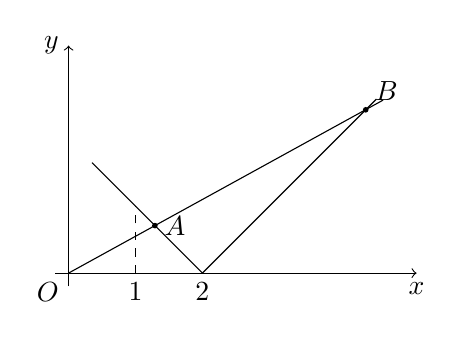
\begin{tikzpicture}[scale=0.85]
\draw[->] (-0.2,0) -- (5.2,0) node[below]{$x$};
\draw[->] (0,-0.2) -- (0,3.4) node[left]{$y$};
\node[below left] at (0,0) {$O$};
\draw (2,0) -- (0.35,1.65);
\draw (2,0) -- (4.6,2.6);
\draw (0,0) -- (4.7,2.585);
\draw[dashed] (1,0) -- (1,1);
\node[below] at (1,0) {$1$};
\node[below] at (2,0) {$2$};
\coordinate (A) at (1.29,0.71); \fill (A) circle (1.2pt); \node[right] at (A) {$A$};
\coordinate (B) at (4.44,2.44); \fill (B) circle (1.2pt); \node[above right] at (B) {$B$};
\end{tikzpicture}
\end{center}
\step{由 $0<k<1$，得 $x_A>1$，}
\step{所以关于 $x$ 的不等式 $k\lvert x\rvert-\lvert x-2\rvert>0$ 恰好有 $4$ 个整数解，是 $2,3,4,5$，}
\step{由 $\begin{cases}y=kx\\ y=x-2\end{cases}\Rightarrow x_B=\dfrac2{1-k}\in(5,6]$，故 $\dfrac35<k\leqslant\dfrac23$.}
\solend
\fi

\item 设集合 $S=\{1,2,3,\cdots,10\}$，$S$ 的子集 $A$ 满足 $A\cap\{1,2,3\}\neq\varnothing$，$A\cup\{4,5,6\}\neq S$，这样的子集 $A$ 的个数为\blankline[4.4em].

\ifanswer
\solbegin
\step{先求使 $A\cap\{1,2,3\}\neq\varnothing$ 成立的 $S$ 的子集 $A$ 的个数 $N_1$，}
\step{在 $\{1,2,3\}$ 中取出至少一个元素的方式有 $7$ 种，}
\step{而集合 $\{4,5,\cdots,10\}$ 的子集有 $2^7$ 个，因此 $N_1=7\times2^7=896$，}
% 注：下一行原卷印作“$A\cup\{4,5,6\}\neq S$”，按上下文应为“$=S$”，照录未改（见文件头“原卷笔误/存疑”①）。
\step{再扣除其中使 $A\cup\{4,5,6\}\neq S$ 的集合 $A$ 的个数 $N_2$，}
\step{这些取法中 $1$，$2$，$3$，$7$，$8$，$9$，$10$ 均被取出，}
\step{而集合 $\{4,5,6\}$ 的子集有 $2^3$ 个，因此 $N_2=2^3=8$，}
\step{从而满足条件的子集 $A$ 的个数为 $N_1-N_2=896-8=888$.}
\solend
\fi

\end{enumerate}

\bigsec{二、选择题}

\begin{enumerate}
\setcounter{enumi}{12}

\item 已知 $a>b$，下列不等式中一定成立是\mbox{（\quad）}

\keepwithprev
A. $a^2>b^2$\qquad B. $ac^2>bc^2$\qquad C. $\dfrac1a<\dfrac1b$\qquad D. $a+3>b-4$

\ifanswer
\solbegin
\step{对于 $A$，当 $a=-2$，$b=-4$ 时，不等式不成立，故 $A$ 错误；}
\step{对于 $B$，当 $c=0$ 时，不等式不成立，故 $B$ 错误；}
\step{对于 $C$，当 $a=2$，$b=-4$ 时，不等式不成立，故 $C$ 错误；}
\step{对于 $D$，因为 $a>b$，$3>-4$，必有 $a+3>b-4$ 成立，故 $D$ 正确.}
\solend
\fi

\item 已知集合 $M$ 满足 $\{2,3\}\subseteq M\subseteq\{1,2,3,4,5\}$，那么这样的集合 $M$ 的个数为\mbox{（\quad）}

\keepwithprev
A. $6$\qquad B. $7$\qquad C. $8$\qquad D. $9$

\ifanswer
\solbegin
\step{集合 $M$ 满足 $\{2,3\}\subseteq M\subseteq\{1,2,3,4,5\}$，所以 $2\in M$，$3\in M$，}
\step{故集合 $M$ 的个数为 $2^3=8$. 故选 $C$.}
\solend
\fi

\item 已知集合 $A=\{x\mid x=2k,k\in\Z\}$，$B=\{x\mid x=4m+6n,m,n\in\Z\}$，则\mbox{（\quad）}

\keepwithprev
A. $B\subset A$\qquad B. $A\subset B$\qquad C. $A=B$\qquad D. $B\neq A$

\ifanswer
\solbegin
\step{$B=\{x\mid x=4m+6n,m,n\in\Z\}$，$B$ 中的元素都是偶数，}
\step{所以 $B$ 的元素都是 $A$ 的元素，$B\subseteq A$；}
\step{$A=\{x\mid x=4(-k)+6k,k\in\Z\}$，则 $A$ 的元素都是 $B$ 的元素，$A\subseteq B$；}
\step{所以 $A=B$. 故选 $C$.}
\solend
\fi

\item 已知集合 $A=[1,a]\cup[a^3,a^4]$，集合 $B=\{x\mid x=x_1-x_2$，其中 $x_1,x_2\in A\}$. 若集合 $B$ 表示的区间为一个闭区间，则 $a$ 的取值范围为\mbox{（\quad）}

\keepwithprev
A. $a$ 取遍任意大于 $1$ 的实数\qquad B. $a\geqslant2$

C. $a\geqslant\dfrac{1+\sqrt5}2$\qquad D. $a\geqslant1+\sqrt2$

\ifanswer
\solbegin
\step{由题意得 $a^3>a>1$，则 $x_1-x_2$ 的最小值为 $1-a^4$，最大值为 $a^4-1$，}
\step{所以 $B=[1-a^4,a^4-1]$，}
\step{又因为 $a^4-a^3-(a-1)=a^3(a-1)-(a-1)=(a^3-1)(a-1)>0$，}
\step{所以 $a^4-a^3>a-1$，又集合 $B$ 表示的区间为一个闭区间，}
\step{则 $a^3-a\leqslant a^4-a^3$，化简得 $a^2-a-1\geqslant0$，又 $a>1$，解得 $a\geqslant\dfrac{1+\sqrt5}2$.}
\step{故选 $C$.}
\solend
\fi

\end{enumerate}

\bigsec{三、解答题}

\begin{enumerate}
\setcounter{enumi}{16}

\item 设全集 $U=\R$，集合 $A=\{x\mid\lvert x+3\rvert\leqslant4\}$，集合 $B=\{x\mid a-2\leqslant x\leqslant1+2a\}$，其中 $a\in\R$.

（1）若 $a=\dfrac12$，求 $A\cap B$；

（2）若 $A\cap B=\varnothing$，求 $a$ 的取值范围.

\ifanswer
\solbegin
\stepm{(1)}{由 $\lvert x+3\rvert\leqslant4$，得 $-4\leqslant x+3\leqslant4$，解得 $-7\leqslant x\leqslant1$，}
\step{所以 $A=\{x\mid-7\leqslant x\leqslant1\}$，}
\step{当 $a=\dfrac12$ 时，$a-2=\dfrac12-2=-\dfrac32$，$1+2a=1+2\times\dfrac12=2$，}
\step{$B=\left\{x\mid-\dfrac32\leqslant x\leqslant2\right\}$，$A\cap B=\left\{x\mid-\dfrac32\leqslant x\leqslant1\right\}$，即 $\left[-\dfrac32,1\right]$.}
\stepm{(2)}{若 $A\cap B=\varnothing$，分两种情况讨论，}
\step{①当 $B\neq\varnothing$ 时，$a-2\leqslant1+2a$，即 $a\geqslant-3$，}
\step{要满足 $A\cap B=\varnothing$，则 $1+2a<-7$ 或 $a-2>1$，}
\step{由 $1+2a<-7$，得 $a<-4$，与 $a\geqslant-3$ 无交集，无解，}
\step{由 $a-2>1$ 得 $a>3$，符合 $a\geqslant-3$，}
\step{②当 $B=\varnothing$ 时，有 $a-2>1+2a$，解得 $a<-3$，满足 $A\cap B=\varnothing$；}
\step{综上，$a$ 的取值范围是 $(-\infty,-3)\cup(3,+\infty)$.}
\solend
\fi

\ansspace

\item （1）已知 $a>b>0$，比较 $\dfrac{a+b}{a^2+b^2}$ 与 $\dfrac1{a-b}$ 的大小并说明理由；

（2）已知 $-2\leqslant x\leqslant-1$，$2\leqslant y\leqslant3$，求 $2x-y$ 的取值范围.

\ifanswer
\solbegin
\stepm{(1)}{$\dfrac{a+b}{a^2+b^2}-\dfrac1{a-b}=\dfrac{(a^2-b^2)-(a^2+b^2)}{(a^2+b^2)(a-b)}=\dfrac{-2b^2}{(a^2+b^2)(a-b)}$，}
\step{因为 $a>b>0$，所以 $a^2(a-b)-b^2(b-a)=(a^2+b^2)(a-b)>0$，}
\step{$\dfrac{-2b^2}{(a^2+b^2)(a-b)}<0$，即 $\dfrac{a+b}{a^2+b^2}-\dfrac1{a-b}<0$，所以 $\dfrac{a+b}{a^2+b^2}<\dfrac1{a-b}$；}
\stepm{(2)}{由 $-2\leqslant x\leqslant-1$，$2\leqslant y\leqslant3$，得 $-4\leqslant2x\leqslant-2$，$-3\leqslant-y\leqslant-2$，}
\step{得 $-7\leqslant2x-y\leqslant-4$，即 $2x-y$ 的取值范围为 $[-7,-4]$.}
\solend
\fi

\ansspace

\item 设 $x_1$、$x_2$ 是关于 $x$ 的方程 $x^2-2(m+2)x+m^2-1=0$ 的两个实数根.

（1）若 $\dfrac1{x_1}+\dfrac1{x_2}=-4$，求 $m$ 的值；

（2）若 $x_1$、$x_2$ 是两个不相等的正数，求实数 $m$ 的取值范围.

\ifanswer
\solbegin
\stepm{(1)}{因为 $x_1$、$x_2$ 是关于 $x$ 的方程的两个实数根，}
\step{所以 $\Delta=(-2(m+2))^2-4(m^2-1)=16m+20\geqslant0$，解得 $m\geqslant-\dfrac54$，}
\step{由韦达定理得 $x_1+x_2=2(m+2)$，$x_1x_2=m^2-1$，}
\step{所以 $\dfrac1{x_1}+\dfrac1{x_2}=\dfrac{x_2+x_1}{x_1x_2}=\dfrac{2(m+2)}{m^2-1}=-4$，即 $2m^2+m=0$，}
\step{解得 $m=0$ 或 $m=-\dfrac12$；}
\stepm{(2)}{由题意得 $\begin{cases}x_1+x_2>0\\ x_1x_2>0\\ \Delta>0\end{cases}$，即 $\begin{cases}2(m+2)>0\\ m^2-1>0\\ (-2(m+2))^2-4(m^2-1)>0\end{cases}$，}
\step{解得 $-\dfrac54<m<-1$ 或 $m>1$.}
\solend
\fi

\ansspace

\ifanswer\else\needvspace{10\baselineskip}\fi
\item 已知集合 $A=\{x\mid x\leqslant2\text{ 或 }x\geqslant a\}$.

（1）若 $B=\left\{x\mid(x-2)\left(x-\dfrac{12}{7-a}\right)<0\right\}$，$A\cap B=\varnothing$，$A\cup B=\R$，求实数 $a$ 的值；

（2）若 $a=3$ 且 $b<2$，$B=\{x\mid x^2-b(b+1)x+b^3<0\}$，$A\cap B\cap\Z$ 的子集个数为 $4$ 个，求实数 $b$ 的取值范围.

\ifanswer
\solbegin
\stepm{(1)}{当 $a\leqslant2$ 时，$A=\{x\mid x\leqslant2\text{ 或 }x\geqslant a\}=\R$，必有 $B=\varnothing$，}
\step{即不等式 $(x-2)\left(x-\dfrac{12}{7-a}\right)<0$ 无解，}
\step{必有 $\dfrac{12}{7-a}=2$，解得 $a=1$，符合题意，}
\step{当 $a>2$ 时，$A=(-\infty,2]\cup[a,+\infty)$，}
\step{若 $A\cap B=\varnothing$，$A\cup B=\R$，则 $B=(2,a)$，}
\step{即方程 $(x-2)\left(x-\dfrac{12}{7-a}\right)=0$ 的两个根是 $2$ 和 $a$，所以 $\dfrac{12}{7-a}=a$，}
\step{解得 $a=3$ 或 $a=4$，符合题意，}
\step{综上，实数 $a$ 的值为 $1$ 或 $3$ 或 $4$；}
\stepm{(2)}{由 $A\cap B\cap\Z$ 的子集个数为 $4$ 个，即 $A\cap B\cap\Z$ 中恰好有 $2$ 个整数元素，}
\step{由 $a=3$，则 $A=(-\infty,2]\cup[3,+\infty)$，}
\step{由 $x^2-b(b+1)x+b^3=(x-b^2)(x-b)<0$，又 $b<2$，}
\step{当 $1<b<2$ 时，$1<b^2<4$ 且 $b^2>b$，则 $B=(b,b^2)$，}
\step{则 $A\cap B=(b,2]\cup[3,b^2)$，}
\step{要使 $A\cap B\cap\Z$ 中恰好有 $2$ 个整数元素，即 $A\cap B\cap\Z=\{2,3\}$，}
\step{即 $\begin{cases}1<b<2\\ 3<b^2<4\end{cases}$，解得 $\sqrt3<b<2$，符合题意，}
\step{当 $b=1$ 或 $b=0$ 时，$B=\varnothing$，此时 $A\cap B\cap\Z=\varnothing$，不符合题意，舍去，}
\step{当 $0<b<1$ 时，$0<b^2<1$ 且 $b^2<b$，则 $B=(b^2,b)$，}
\step{此时 $A\cap B\cap\Z=\varnothing$，不符合题意，舍去，}
\step{当 $-1<b<0$ 时，$0<b^2<1$ 且 $b^2>b$，则 $B=(b,b^2)$，}
\step{此时 $A\cap B\cap\Z=\{0\}$，即 $A\cap B\cap\Z$ 中只有 $1$ 个元素，不符合题意，舍去，}
\step{当 $b\leqslant-1$ 时，$b^2\geqslant1$ 且 $b^2>b$，则 $B=(b,b^2)$，}
\step{此时 $A\cap B\cap\Z\supseteq\{-1,0,1\}$，即 $A\cap B\cap\Z$ 中至少有 $3$ 个元素，}
\step{不符合题意，舍去，}
\step{综上，实数 $b$ 的取值范围为 $(\sqrt3,2)$.}
\solend
\fi

\ansspace*[7]

\item 已知集合 $A=\{a_1,a_2,a_3,\cdots,a_n\}$ 中的元素均为正整数，其中 $n\in\N$ 且 $n\geqslant3$. 若对任意 $x,y\in A(x\neq y)$，都有 $\lvert x-y\rvert\geqslant\dfrac{xy}k$，则称集合 $A$ 具有性质 $M_k$.

（1）集合 $A=\{1,2,a\}$ 具有性质 $M_3$，求 $a$ 的最小值；

（2）若集合 $A$ 具有性质 $M_{24}$，且 $A$ 中最小元素和最大元素分别为 $a,b$，求证：$\dfrac1a-\dfrac1b\geqslant\dfrac{n-1}{24}$；

（3）已知集合 $A$ 具有性质 $M_{24}$，求 $A$ 中元素个数的最大值，并说明理由.

\ifanswer
\solbegin
\stepm{(1)}{由性质 $M_3$ 定义得 $\begin{cases}a-1\geqslant\dfrac a3\\ a-2\geqslant\dfrac{2a}3\end{cases}\Rightarrow\begin{cases}a\geqslant\dfrac32\\ a\geqslant6\end{cases}\Rightarrow a\geqslant6$，且 $a\subseteq\N^*$，}
% 注：上一行原卷印作“$a\subseteq\N^*$”，应为“$a\in\N^*$”，照录未改（见文件头“原卷笔误/存疑”②）。
\step{所以 $a$ 的最小值为 $6$.}
\stepm{(2)}{由题意得 $\lvert a_i-a_{i+1}\rvert\geqslant\dfrac{a_ia_{i+1}}{24}$，$(i=1,2,3,\cdots,n-1)$，且 $a_1<\cdots<a_n$，}
\step{所以 $a_{i+1}-a_i\geqslant\dfrac{a_ia_{i+1}}{24}\Rightarrow\dfrac1{a_i}-\dfrac1{a_{i+1}}\geqslant\dfrac1{24}$，$(i=1,2,3,\cdots,n-1)$，}
\step{所以 $\dfrac1{a_1}-\dfrac1{a_2}+\dfrac1{a_2}-\dfrac1{a_3}+\cdots+\dfrac1{a_{n-1}}-\dfrac1{a_n}=\dfrac1{a_1}-\dfrac1{a_n}\geqslant\dfrac{n-1}{24}$，得证.}
\stepm{(3)}{由 (2) 得 $\begin{cases}\dfrac1{a_1}\geqslant\dfrac{n-1}{24}\\ a_1\geqslant1\end{cases}\Rightarrow\dfrac{n-1}{24}<1\Rightarrow n<25$，}
\step{同 (2) 证明得 $\dfrac1{a_i}-\dfrac1{a_n}\geqslant\dfrac{n-i}{24}$ 且 $i=1,2,3,\cdots,n-1$，故 $\dfrac1{a_i}>\dfrac{n-i}{24}$，}
\step{又 $a_i\geqslant i$，所以 $\dfrac1i>\dfrac{n-i}{24}\Rightarrow i(n-i)<24$ 在 $i=1,2,3,\cdots,n-1$ 上恒成立，}
\step{当 $n\geqslant10$，取 $i=5$，则 $i(n-i)=5(n-5)>24$，故 $n<10$，}
\step{当 $n\leqslant9$，则 $i(n-i)\leqslant\dfrac{(i+n-i)^2}4=\dfrac{n^2}4<24\Rightarrow n<\sqrt{96}$，即 $n\leqslant9$.}
\step{综上，集合 $A$ 中元素个数的最大值为 $9$.}
\solend
\fi

\end{enumerate}

\end{document}
"
% 紧凑版：xelatex "\def\iscompact{1}% 高一79_南汇中学_10月月考.tex
%   —— 高一上数学“2026-2027 年南汇中学高一上 10 月月考”（讲评版）
% 试卷版：xelatex 高一79_南汇中学_10月月考.tex
% 答案版：xelatex "\def\isanswer{1}\input{高一79_南汇中学_10月月考.tex}"
% 紧凑版：xelatex "\def\iscompact{1}\input{高一79_南汇中学_10月月考.tex}"
%
% 原始材料：微信公众号“魔都数学加油站”文章，连载“27学年高一79”；
% 原文标题“27学年高一79——2026-2027年上海市南汇中学高一上10月月考”；
% 原文链接：https://mp.weixin.qq.com/s/bFvc7GVgPTaDGg_6JSSfGg。
% 页面标注发布时间 2026-10-24 21:00（上海）。
% 正文为 9 张 PNG 页（`原图/高一79_南汇中学_10月月考/01..09.png`），
% 尺寸混排（第 1、2、4、5、7、8 页为 4762×6735，第 3、6、9 页为 2560×3620），均按页序读取。
%
% 篇幅与题号：原卷自第 3 题起编号。填空题 3—12（10 题）、选择题 13—16（4 题）、
% 解答题 17—21（5 题），共 19 题。
%
% 讲评版：第 4 题只印【答案】，本稿只给 \ans{}；其余 18 题印【解析】。
% 选择题答案在解析末句“故选 D／C／C／C”。
%
% 副标题：原卷未印副标题。本稿按内容标作“集合与常用逻辑用语、不等式”。
%
% 原卷笔误/存疑（均照录未改，正文对应处另有 % 注）：
%   ① 第 12 题解析作“再扣除其中使 $A\cup\{4,5,6\}\neq S$ 的集合 $A$ 的个数 $N_2$”，
%      按上下文应为“$A\cup\{4,5,6\}=S$”，否则“这些取法中 $1,2,3,7,8,9,10$ 均被取出”
%      与 $N_2=2^3=8$ 都无法解释；原卷印作 $\neq$，照录未改。
%   ② 第 21 题 (1) 解析末作“且 $a\subseteq\N^*$”，$a$ 是集合的元素，应为 $a\in\N^*$；
%      原卷印作 $\subseteq$，照录未改。
%
% 与原卷的排版差异：
%   ① 原卷每题下直接印【答案】/【解析】，本稿按全稿惯例将答案与解析置于答案版；
%   ② 原卷未印副标题，本稿补出；填空横线统一排 \blankline[4.4em]；
%   ③ 原卷数集记号排斜体 $R$、$Z$、$N$，本稿按全稿惯例改用 $\R$、$\Z$、$\N$；
%   ④ 第 17—21 题的子问用行内“（1）（2）（3）”段，解析中的子问标号用 \stepm；
%   ⑤ 解答题按惯例加 \ansspace；选择题括号排 \mbox{（\quad）}；
%   ⑥ 第 11 题解析有一幅函数图象（$y=k\lvert x\rvert$ 与 $y=\lvert x-2\rvert$），
%      按原图形状用 TikZ 重排（仅答案版出）。
%
% 行数核对：逐题数 \step/\stepm 条数，合计 107 条（Q3：2；Q5：2；Q6：1；Q7：4；Q8：4；
% Q9：4；Q10：5；Q11：4；Q12：7；Q13：4；Q14：2；Q15：4；Q16：6；Q17：11；Q18：5；
% Q19：7；Q20：24；Q21：11）。原卷解析的换行按语意合并，未逐行强拆；第 4 题只印
% 【答案】，提 \ans{}，不计入 \step 账。
%
\documentclass[a4paper,11pt]{article}
\usepackage{common}

\begin{document}

\examtitlest[3]{2026--2027 年南汇中学高一上 10 月月考}{集合与常用逻辑用语、不等式}

\bigsec{一、填空题}

\begin{enumerate}
\setcounter{enumi}{2}

\item 不等式 $\dfrac{1-x}{x}>0$ 的解集为\blankline[4.4em].

\ifanswer
\solbegin
\step{原不等式化为 $x(x-1)<0$，转化为 $\begin{cases}x>0\\ x-1<0\end{cases}$ 或 $\begin{cases}x<0\\ x-1>0\end{cases}$，}
\step{解得 $0<x<1$，则不等式的解集为 $\{x\mid0<x<1\}$.}
\solend
\fi

\item 用反证法证明命题：“若 $x^2<1$，则 $-1<x<1$”时，应假设\blankline[4.4em].

\ifanswer
\ans{$x\geqslant1$ 或 $x\leqslant-1$}
\fi

\item 设 $k$ 为实数，关于 $x$ 的不等式 $kx^2+x+2<0$ 的解集为 $A$，若 $2\notin A$，则 $k$ 的取值范围是\blankline[4.4em].

\ifanswer
\solbegin
\step{因为关于 $x$ 的不等式 $kx^2+x+2<0$ 的解集为 $A$，且 $2\notin A$，}
\step{所以 $x=2$ 时，$k\times2^2+2+2\geqslant0$，解得 $k\geqslant-1$，则 $k$ 的取值范围为 $[-1,+\infty)$.}
\solend
\fi

\item 已知集合 $M=\{y\mid y=x^2-2x,x\in\R\}$，$N=\{x\mid y=\sqrt{4-x^2}\}$，则 $M\cup N=$\blankline[4.4em].

\ifanswer
\solbegin
\step{$M=[-1,+\infty)$，$N=[-2,2]$，则 $M\cup N=[-2,+\infty)$.}
\solend
\fi

\item 设集合 $A=\{-3,2\}$，集合 $B=\{x\mid mx+1=0\}$，且 $A\cup B=A$，则 $m$ 的值组成的集合是\blankline[4.4em].

\ifanswer
\solbegin
\step{由 $A\cup B=A$，得 $B\subseteq A$，}
\step{当 $m=0$ 时，$B=\varnothing$，满足题意，}
\step{当 $m\neq0$ 时，$B=\left\{-\dfrac1m\right\}$，所以 $-\dfrac1m=2$ 或 $-\dfrac1m=-3$，所以 $m=-\dfrac12$ 或 $m=\dfrac13$，}
\step{综上所述，$m$ 的值组成的集合是 $\left\{0,-\dfrac12,\dfrac13\right\}$.}
\solend
\fi

\item 若不等式 $\lvert x\rvert<a$ 的一个充分不必要条件为 $\dfrac{2x-1}{x-2}<1$，则实数 $a$ 的取值范围是\blankline[4.4em].

\ifanswer
\solbegin
\step{不等式 $\lvert x\rvert<a$，得 $-a<x<a$，}
\step{不等式 $\dfrac{2x-1}{x-2}<1$，即 $\dfrac{2x-1-(x-2)}{x-2}=\dfrac{x+1}{x-2}<0$，解得 $-1<x<2$，}
\step{又不等式 $\lvert x\rvert<a$ 的一个充分不必要条件为 $\dfrac{2x-1}{x-2}<1$，}
\step{得 $\begin{cases}a\geqslant2\\ -a\leqslant-1\end{cases}$，且两等号不同时成立，解得 $a\geqslant2$.}
\solend
\fi

\item 若对任意 $x\in\R$ 都有 $(m-1)x^2-(m-1)x-1<0$，则实数 $m$ 的取值范围是\blankline[4.4em].

\ifanswer
\solbegin
\step{当 $m-1\neq0$，即 $m\neq1$ 时，则有 $\begin{cases}m-1<0\\ (m-1)^2-4(m-1)\times(-1)<0\end{cases}$，}
\step{解得 $-3<m<1$；}
\step{当 $m-1=0$ 时，即当 $m=1$ 时，此时不等式为 $-1<0$ 恒成立，符合题意；}
\step{综上所述，实数 $m$ 的取值范围是 $(-3,1]$.}
\solend
\fi

\item 关于 $x$ 的方程 $\dfrac{x}{x-1}=\dfrac{k-x}{x^2-x}$ 的解集中只含有一个元素，则 $k$ 的可能取值构成的集合为\blankline[4.4em].

\ifanswer
\solbegin
\step{方程两边同时乘以 $x(x-1)$ 得 $x^2=k-x$，即 $x^2+x-k=0$，}
\step{①当其中一个解为增根时，方程也只有一个解，}
\step{(i) 若增根为 $0$ 时，$k=0$；(ii) 若增根为 $1$ 时，$k=2$；}
\step{②当 $\Delta=1+4k=0$，即 $k=-\dfrac14$ 时，方程 $x^2+x-k=0$ 只有一个解；}
\step{即 $k$ 的可能取值构成的集合为 $\left\{-\dfrac14,0,2\right\}$.}
\solend
\fi

\item 若关于 $x$ 的不等式 $k\lvert x\rvert>\lvert x-2\rvert$ 恰好有 $4$ 个整数解，则实数 $k$ 的取值范围是\blankline[4.4em].

\ifanswer
\solbegin
\step{由题意得 $0<k<1$，函数 $y=k\lvert x\rvert$ 与 $y=\lvert x-2\rvert$ 的图象如图：}
\begin{center}
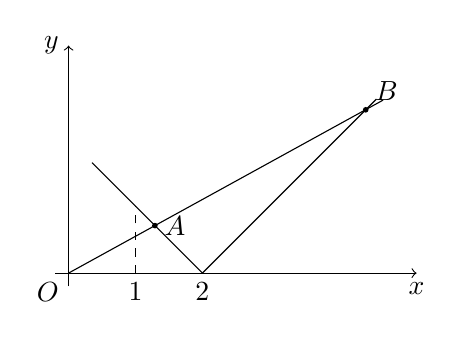
\begin{tikzpicture}[scale=0.85]
\draw[->] (-0.2,0) -- (5.2,0) node[below]{$x$};
\draw[->] (0,-0.2) -- (0,3.4) node[left]{$y$};
\node[below left] at (0,0) {$O$};
\draw (2,0) -- (0.35,1.65);
\draw (2,0) -- (4.6,2.6);
\draw (0,0) -- (4.7,2.585);
\draw[dashed] (1,0) -- (1,1);
\node[below] at (1,0) {$1$};
\node[below] at (2,0) {$2$};
\coordinate (A) at (1.29,0.71); \fill (A) circle (1.2pt); \node[right] at (A) {$A$};
\coordinate (B) at (4.44,2.44); \fill (B) circle (1.2pt); \node[above right] at (B) {$B$};
\end{tikzpicture}
\end{center}
\step{由 $0<k<1$，得 $x_A>1$，}
\step{所以关于 $x$ 的不等式 $k\lvert x\rvert-\lvert x-2\rvert>0$ 恰好有 $4$ 个整数解，是 $2,3,4,5$，}
\step{由 $\begin{cases}y=kx\\ y=x-2\end{cases}\Rightarrow x_B=\dfrac2{1-k}\in(5,6]$，故 $\dfrac35<k\leqslant\dfrac23$.}
\solend
\fi

\item 设集合 $S=\{1,2,3,\cdots,10\}$，$S$ 的子集 $A$ 满足 $A\cap\{1,2,3\}\neq\varnothing$，$A\cup\{4,5,6\}\neq S$，这样的子集 $A$ 的个数为\blankline[4.4em].

\ifanswer
\solbegin
\step{先求使 $A\cap\{1,2,3\}\neq\varnothing$ 成立的 $S$ 的子集 $A$ 的个数 $N_1$，}
\step{在 $\{1,2,3\}$ 中取出至少一个元素的方式有 $7$ 种，}
\step{而集合 $\{4,5,\cdots,10\}$ 的子集有 $2^7$ 个，因此 $N_1=7\times2^7=896$，}
% 注：下一行原卷印作“$A\cup\{4,5,6\}\neq S$”，按上下文应为“$=S$”，照录未改（见文件头“原卷笔误/存疑”①）。
\step{再扣除其中使 $A\cup\{4,5,6\}\neq S$ 的集合 $A$ 的个数 $N_2$，}
\step{这些取法中 $1$，$2$，$3$，$7$，$8$，$9$，$10$ 均被取出，}
\step{而集合 $\{4,5,6\}$ 的子集有 $2^3$ 个，因此 $N_2=2^3=8$，}
\step{从而满足条件的子集 $A$ 的个数为 $N_1-N_2=896-8=888$.}
\solend
\fi

\end{enumerate}

\bigsec{二、选择题}

\begin{enumerate}
\setcounter{enumi}{12}

\item 已知 $a>b$，下列不等式中一定成立是\mbox{（\quad）}

\keepwithprev
A. $a^2>b^2$\qquad B. $ac^2>bc^2$\qquad C. $\dfrac1a<\dfrac1b$\qquad D. $a+3>b-4$

\ifanswer
\solbegin
\step{对于 $A$，当 $a=-2$，$b=-4$ 时，不等式不成立，故 $A$ 错误；}
\step{对于 $B$，当 $c=0$ 时，不等式不成立，故 $B$ 错误；}
\step{对于 $C$，当 $a=2$，$b=-4$ 时，不等式不成立，故 $C$ 错误；}
\step{对于 $D$，因为 $a>b$，$3>-4$，必有 $a+3>b-4$ 成立，故 $D$ 正确.}
\solend
\fi

\item 已知集合 $M$ 满足 $\{2,3\}\subseteq M\subseteq\{1,2,3,4,5\}$，那么这样的集合 $M$ 的个数为\mbox{（\quad）}

\keepwithprev
A. $6$\qquad B. $7$\qquad C. $8$\qquad D. $9$

\ifanswer
\solbegin
\step{集合 $M$ 满足 $\{2,3\}\subseteq M\subseteq\{1,2,3,4,5\}$，所以 $2\in M$，$3\in M$，}
\step{故集合 $M$ 的个数为 $2^3=8$. 故选 $C$.}
\solend
\fi

\item 已知集合 $A=\{x\mid x=2k,k\in\Z\}$，$B=\{x\mid x=4m+6n,m,n\in\Z\}$，则\mbox{（\quad）}

\keepwithprev
A. $B\subset A$\qquad B. $A\subset B$\qquad C. $A=B$\qquad D. $B\neq A$

\ifanswer
\solbegin
\step{$B=\{x\mid x=4m+6n,m,n\in\Z\}$，$B$ 中的元素都是偶数，}
\step{所以 $B$ 的元素都是 $A$ 的元素，$B\subseteq A$；}
\step{$A=\{x\mid x=4(-k)+6k,k\in\Z\}$，则 $A$ 的元素都是 $B$ 的元素，$A\subseteq B$；}
\step{所以 $A=B$. 故选 $C$.}
\solend
\fi

\item 已知集合 $A=[1,a]\cup[a^3,a^4]$，集合 $B=\{x\mid x=x_1-x_2$，其中 $x_1,x_2\in A\}$. 若集合 $B$ 表示的区间为一个闭区间，则 $a$ 的取值范围为\mbox{（\quad）}

\keepwithprev
A. $a$ 取遍任意大于 $1$ 的实数\qquad B. $a\geqslant2$

C. $a\geqslant\dfrac{1+\sqrt5}2$\qquad D. $a\geqslant1+\sqrt2$

\ifanswer
\solbegin
\step{由题意得 $a^3>a>1$，则 $x_1-x_2$ 的最小值为 $1-a^4$，最大值为 $a^4-1$，}
\step{所以 $B=[1-a^4,a^4-1]$，}
\step{又因为 $a^4-a^3-(a-1)=a^3(a-1)-(a-1)=(a^3-1)(a-1)>0$，}
\step{所以 $a^4-a^3>a-1$，又集合 $B$ 表示的区间为一个闭区间，}
\step{则 $a^3-a\leqslant a^4-a^3$，化简得 $a^2-a-1\geqslant0$，又 $a>1$，解得 $a\geqslant\dfrac{1+\sqrt5}2$.}
\step{故选 $C$.}
\solend
\fi

\end{enumerate}

\bigsec{三、解答题}

\begin{enumerate}
\setcounter{enumi}{16}

\item 设全集 $U=\R$，集合 $A=\{x\mid\lvert x+3\rvert\leqslant4\}$，集合 $B=\{x\mid a-2\leqslant x\leqslant1+2a\}$，其中 $a\in\R$.

（1）若 $a=\dfrac12$，求 $A\cap B$；

（2）若 $A\cap B=\varnothing$，求 $a$ 的取值范围.

\ifanswer
\solbegin
\stepm{(1)}{由 $\lvert x+3\rvert\leqslant4$，得 $-4\leqslant x+3\leqslant4$，解得 $-7\leqslant x\leqslant1$，}
\step{所以 $A=\{x\mid-7\leqslant x\leqslant1\}$，}
\step{当 $a=\dfrac12$ 时，$a-2=\dfrac12-2=-\dfrac32$，$1+2a=1+2\times\dfrac12=2$，}
\step{$B=\left\{x\mid-\dfrac32\leqslant x\leqslant2\right\}$，$A\cap B=\left\{x\mid-\dfrac32\leqslant x\leqslant1\right\}$，即 $\left[-\dfrac32,1\right]$.}
\stepm{(2)}{若 $A\cap B=\varnothing$，分两种情况讨论，}
\step{①当 $B\neq\varnothing$ 时，$a-2\leqslant1+2a$，即 $a\geqslant-3$，}
\step{要满足 $A\cap B=\varnothing$，则 $1+2a<-7$ 或 $a-2>1$，}
\step{由 $1+2a<-7$，得 $a<-4$，与 $a\geqslant-3$ 无交集，无解，}
\step{由 $a-2>1$ 得 $a>3$，符合 $a\geqslant-3$，}
\step{②当 $B=\varnothing$ 时，有 $a-2>1+2a$，解得 $a<-3$，满足 $A\cap B=\varnothing$；}
\step{综上，$a$ 的取值范围是 $(-\infty,-3)\cup(3,+\infty)$.}
\solend
\fi

\ansspace

\item （1）已知 $a>b>0$，比较 $\dfrac{a+b}{a^2+b^2}$ 与 $\dfrac1{a-b}$ 的大小并说明理由；

（2）已知 $-2\leqslant x\leqslant-1$，$2\leqslant y\leqslant3$，求 $2x-y$ 的取值范围.

\ifanswer
\solbegin
\stepm{(1)}{$\dfrac{a+b}{a^2+b^2}-\dfrac1{a-b}=\dfrac{(a^2-b^2)-(a^2+b^2)}{(a^2+b^2)(a-b)}=\dfrac{-2b^2}{(a^2+b^2)(a-b)}$，}
\step{因为 $a>b>0$，所以 $a^2(a-b)-b^2(b-a)=(a^2+b^2)(a-b)>0$，}
\step{$\dfrac{-2b^2}{(a^2+b^2)(a-b)}<0$，即 $\dfrac{a+b}{a^2+b^2}-\dfrac1{a-b}<0$，所以 $\dfrac{a+b}{a^2+b^2}<\dfrac1{a-b}$；}
\stepm{(2)}{由 $-2\leqslant x\leqslant-1$，$2\leqslant y\leqslant3$，得 $-4\leqslant2x\leqslant-2$，$-3\leqslant-y\leqslant-2$，}
\step{得 $-7\leqslant2x-y\leqslant-4$，即 $2x-y$ 的取值范围为 $[-7,-4]$.}
\solend
\fi

\ansspace

\item 设 $x_1$、$x_2$ 是关于 $x$ 的方程 $x^2-2(m+2)x+m^2-1=0$ 的两个实数根.

（1）若 $\dfrac1{x_1}+\dfrac1{x_2}=-4$，求 $m$ 的值；

（2）若 $x_1$、$x_2$ 是两个不相等的正数，求实数 $m$ 的取值范围.

\ifanswer
\solbegin
\stepm{(1)}{因为 $x_1$、$x_2$ 是关于 $x$ 的方程的两个实数根，}
\step{所以 $\Delta=(-2(m+2))^2-4(m^2-1)=16m+20\geqslant0$，解得 $m\geqslant-\dfrac54$，}
\step{由韦达定理得 $x_1+x_2=2(m+2)$，$x_1x_2=m^2-1$，}
\step{所以 $\dfrac1{x_1}+\dfrac1{x_2}=\dfrac{x_2+x_1}{x_1x_2}=\dfrac{2(m+2)}{m^2-1}=-4$，即 $2m^2+m=0$，}
\step{解得 $m=0$ 或 $m=-\dfrac12$；}
\stepm{(2)}{由题意得 $\begin{cases}x_1+x_2>0\\ x_1x_2>0\\ \Delta>0\end{cases}$，即 $\begin{cases}2(m+2)>0\\ m^2-1>0\\ (-2(m+2))^2-4(m^2-1)>0\end{cases}$，}
\step{解得 $-\dfrac54<m<-1$ 或 $m>1$.}
\solend
\fi

\ansspace

\ifanswer\else\needvspace{10\baselineskip}\fi
\item 已知集合 $A=\{x\mid x\leqslant2\text{ 或 }x\geqslant a\}$.

（1）若 $B=\left\{x\mid(x-2)\left(x-\dfrac{12}{7-a}\right)<0\right\}$，$A\cap B=\varnothing$，$A\cup B=\R$，求实数 $a$ 的值；

（2）若 $a=3$ 且 $b<2$，$B=\{x\mid x^2-b(b+1)x+b^3<0\}$，$A\cap B\cap\Z$ 的子集个数为 $4$ 个，求实数 $b$ 的取值范围.

\ifanswer
\solbegin
\stepm{(1)}{当 $a\leqslant2$ 时，$A=\{x\mid x\leqslant2\text{ 或 }x\geqslant a\}=\R$，必有 $B=\varnothing$，}
\step{即不等式 $(x-2)\left(x-\dfrac{12}{7-a}\right)<0$ 无解，}
\step{必有 $\dfrac{12}{7-a}=2$，解得 $a=1$，符合题意，}
\step{当 $a>2$ 时，$A=(-\infty,2]\cup[a,+\infty)$，}
\step{若 $A\cap B=\varnothing$，$A\cup B=\R$，则 $B=(2,a)$，}
\step{即方程 $(x-2)\left(x-\dfrac{12}{7-a}\right)=0$ 的两个根是 $2$ 和 $a$，所以 $\dfrac{12}{7-a}=a$，}
\step{解得 $a=3$ 或 $a=4$，符合题意，}
\step{综上，实数 $a$ 的值为 $1$ 或 $3$ 或 $4$；}
\stepm{(2)}{由 $A\cap B\cap\Z$ 的子集个数为 $4$ 个，即 $A\cap B\cap\Z$ 中恰好有 $2$ 个整数元素，}
\step{由 $a=3$，则 $A=(-\infty,2]\cup[3,+\infty)$，}
\step{由 $x^2-b(b+1)x+b^3=(x-b^2)(x-b)<0$，又 $b<2$，}
\step{当 $1<b<2$ 时，$1<b^2<4$ 且 $b^2>b$，则 $B=(b,b^2)$，}
\step{则 $A\cap B=(b,2]\cup[3,b^2)$，}
\step{要使 $A\cap B\cap\Z$ 中恰好有 $2$ 个整数元素，即 $A\cap B\cap\Z=\{2,3\}$，}
\step{即 $\begin{cases}1<b<2\\ 3<b^2<4\end{cases}$，解得 $\sqrt3<b<2$，符合题意，}
\step{当 $b=1$ 或 $b=0$ 时，$B=\varnothing$，此时 $A\cap B\cap\Z=\varnothing$，不符合题意，舍去，}
\step{当 $0<b<1$ 时，$0<b^2<1$ 且 $b^2<b$，则 $B=(b^2,b)$，}
\step{此时 $A\cap B\cap\Z=\varnothing$，不符合题意，舍去，}
\step{当 $-1<b<0$ 时，$0<b^2<1$ 且 $b^2>b$，则 $B=(b,b^2)$，}
\step{此时 $A\cap B\cap\Z=\{0\}$，即 $A\cap B\cap\Z$ 中只有 $1$ 个元素，不符合题意，舍去，}
\step{当 $b\leqslant-1$ 时，$b^2\geqslant1$ 且 $b^2>b$，则 $B=(b,b^2)$，}
\step{此时 $A\cap B\cap\Z\supseteq\{-1,0,1\}$，即 $A\cap B\cap\Z$ 中至少有 $3$ 个元素，}
\step{不符合题意，舍去，}
\step{综上，实数 $b$ 的取值范围为 $(\sqrt3,2)$.}
\solend
\fi

\ansspace*[7]

\item 已知集合 $A=\{a_1,a_2,a_3,\cdots,a_n\}$ 中的元素均为正整数，其中 $n\in\N$ 且 $n\geqslant3$. 若对任意 $x,y\in A(x\neq y)$，都有 $\lvert x-y\rvert\geqslant\dfrac{xy}k$，则称集合 $A$ 具有性质 $M_k$.

（1）集合 $A=\{1,2,a\}$ 具有性质 $M_3$，求 $a$ 的最小值；

（2）若集合 $A$ 具有性质 $M_{24}$，且 $A$ 中最小元素和最大元素分别为 $a,b$，求证：$\dfrac1a-\dfrac1b\geqslant\dfrac{n-1}{24}$；

（3）已知集合 $A$ 具有性质 $M_{24}$，求 $A$ 中元素个数的最大值，并说明理由.

\ifanswer
\solbegin
\stepm{(1)}{由性质 $M_3$ 定义得 $\begin{cases}a-1\geqslant\dfrac a3\\ a-2\geqslant\dfrac{2a}3\end{cases}\Rightarrow\begin{cases}a\geqslant\dfrac32\\ a\geqslant6\end{cases}\Rightarrow a\geqslant6$，且 $a\subseteq\N^*$，}
% 注：上一行原卷印作“$a\subseteq\N^*$”，应为“$a\in\N^*$”，照录未改（见文件头“原卷笔误/存疑”②）。
\step{所以 $a$ 的最小值为 $6$.}
\stepm{(2)}{由题意得 $\lvert a_i-a_{i+1}\rvert\geqslant\dfrac{a_ia_{i+1}}{24}$，$(i=1,2,3,\cdots,n-1)$，且 $a_1<\cdots<a_n$，}
\step{所以 $a_{i+1}-a_i\geqslant\dfrac{a_ia_{i+1}}{24}\Rightarrow\dfrac1{a_i}-\dfrac1{a_{i+1}}\geqslant\dfrac1{24}$，$(i=1,2,3,\cdots,n-1)$，}
\step{所以 $\dfrac1{a_1}-\dfrac1{a_2}+\dfrac1{a_2}-\dfrac1{a_3}+\cdots+\dfrac1{a_{n-1}}-\dfrac1{a_n}=\dfrac1{a_1}-\dfrac1{a_n}\geqslant\dfrac{n-1}{24}$，得证.}
\stepm{(3)}{由 (2) 得 $\begin{cases}\dfrac1{a_1}\geqslant\dfrac{n-1}{24}\\ a_1\geqslant1\end{cases}\Rightarrow\dfrac{n-1}{24}<1\Rightarrow n<25$，}
\step{同 (2) 证明得 $\dfrac1{a_i}-\dfrac1{a_n}\geqslant\dfrac{n-i}{24}$ 且 $i=1,2,3,\cdots,n-1$，故 $\dfrac1{a_i}>\dfrac{n-i}{24}$，}
\step{又 $a_i\geqslant i$，所以 $\dfrac1i>\dfrac{n-i}{24}\Rightarrow i(n-i)<24$ 在 $i=1,2,3,\cdots,n-1$ 上恒成立，}
\step{当 $n\geqslant10$，取 $i=5$，则 $i(n-i)=5(n-5)>24$，故 $n<10$，}
\step{当 $n\leqslant9$，则 $i(n-i)\leqslant\dfrac{(i+n-i)^2}4=\dfrac{n^2}4<24\Rightarrow n<\sqrt{96}$，即 $n\leqslant9$.}
\step{综上，集合 $A$ 中元素个数的最大值为 $9$.}
\solend
\fi

\end{enumerate}

\end{document}
"
%
% 原始材料：微信公众号“魔都数学加油站”文章，连载“27学年高一79”；
% 原文标题“27学年高一79——2026-2027年上海市南汇中学高一上10月月考”；
% 原文链接：https://mp.weixin.qq.com/s/bFvc7GVgPTaDGg_6JSSfGg。
% 页面标注发布时间 2026-10-24 21:00（上海）。
% 正文为 9 张 PNG 页（`原图/高一79_南汇中学_10月月考/01..09.png`），
% 尺寸混排（第 1、2、4、5、7、8 页为 4762×6735，第 3、6、9 页为 2560×3620），均按页序读取。
%
% 篇幅与题号：原卷自第 3 题起编号。填空题 3—12（10 题）、选择题 13—16（4 题）、
% 解答题 17—21（5 题），共 19 题。
%
% 讲评版：第 4 题只印【答案】，本稿只给 \ans{}；其余 18 题印【解析】。
% 选择题答案在解析末句“故选 D／C／C／C”。
%
% 副标题：原卷未印副标题。本稿按内容标作“集合与常用逻辑用语、不等式”。
%
% 原卷笔误/存疑（均照录未改，正文对应处另有 % 注）：
%   ① 第 12 题解析作“再扣除其中使 $A\cup\{4,5,6\}\neq S$ 的集合 $A$ 的个数 $N_2$”，
%      按上下文应为“$A\cup\{4,5,6\}=S$”，否则“这些取法中 $1,2,3,7,8,9,10$ 均被取出”
%      与 $N_2=2^3=8$ 都无法解释；原卷印作 $\neq$，照录未改。
%   ② 第 21 题 (1) 解析末作“且 $a\subseteq\N^*$”，$a$ 是集合的元素，应为 $a\in\N^*$；
%      原卷印作 $\subseteq$，照录未改。
%
% 与原卷的排版差异：
%   ① 原卷每题下直接印【答案】/【解析】，本稿按全稿惯例将答案与解析置于答案版；
%   ② 原卷未印副标题，本稿补出；填空横线统一排 \blankline[4.4em]；
%   ③ 原卷数集记号排斜体 $R$、$Z$、$N$，本稿按全稿惯例改用 $\R$、$\Z$、$\N$；
%   ④ 第 17—21 题的子问用行内“（1）（2）（3）”段，解析中的子问标号用 \stepm；
%   ⑤ 解答题按惯例加 \ansspace；选择题括号排 \mbox{（\quad）}；
%   ⑥ 第 11 题解析有一幅函数图象（$y=k\lvert x\rvert$ 与 $y=\lvert x-2\rvert$），
%      按原图形状用 TikZ 重排（仅答案版出）。
%
% 行数核对：逐题数 \step/\stepm 条数，合计 107 条（Q3：2；Q5：2；Q6：1；Q7：4；Q8：4；
% Q9：4；Q10：5；Q11：4；Q12：7；Q13：4；Q14：2；Q15：4；Q16：6；Q17：11；Q18：5；
% Q19：7；Q20：24；Q21：11）。原卷解析的换行按语意合并，未逐行强拆；第 4 题只印
% 【答案】，提 \ans{}，不计入 \step 账。
%
\documentclass[a4paper,11pt]{article}
\usepackage{common}

\begin{document}

\examtitlest[3]{2026--2027 年南汇中学高一上 10 月月考}{集合与常用逻辑用语、不等式}

\bigsec{一、填空题}

\begin{enumerate}
\setcounter{enumi}{2}

\item 不等式 $\dfrac{1-x}{x}>0$ 的解集为\blankline[4.4em].

\ifanswer
\solbegin
\step{原不等式化为 $x(x-1)<0$，转化为 $\begin{cases}x>0\\ x-1<0\end{cases}$ 或 $\begin{cases}x<0\\ x-1>0\end{cases}$，}
\step{解得 $0<x<1$，则不等式的解集为 $\{x\mid0<x<1\}$.}
\solend
\fi

\item 用反证法证明命题：“若 $x^2<1$，则 $-1<x<1$”时，应假设\blankline[4.4em].

\ifanswer
\ans{$x\geqslant1$ 或 $x\leqslant-1$}
\fi

\item 设 $k$ 为实数，关于 $x$ 的不等式 $kx^2+x+2<0$ 的解集为 $A$，若 $2\notin A$，则 $k$ 的取值范围是\blankline[4.4em].

\ifanswer
\solbegin
\step{因为关于 $x$ 的不等式 $kx^2+x+2<0$ 的解集为 $A$，且 $2\notin A$，}
\step{所以 $x=2$ 时，$k\times2^2+2+2\geqslant0$，解得 $k\geqslant-1$，则 $k$ 的取值范围为 $[-1,+\infty)$.}
\solend
\fi

\item 已知集合 $M=\{y\mid y=x^2-2x,x\in\R\}$，$N=\{x\mid y=\sqrt{4-x^2}\}$，则 $M\cup N=$\blankline[4.4em].

\ifanswer
\solbegin
\step{$M=[-1,+\infty)$，$N=[-2,2]$，则 $M\cup N=[-2,+\infty)$.}
\solend
\fi

\item 设集合 $A=\{-3,2\}$，集合 $B=\{x\mid mx+1=0\}$，且 $A\cup B=A$，则 $m$ 的值组成的集合是\blankline[4.4em].

\ifanswer
\solbegin
\step{由 $A\cup B=A$，得 $B\subseteq A$，}
\step{当 $m=0$ 时，$B=\varnothing$，满足题意，}
\step{当 $m\neq0$ 时，$B=\left\{-\dfrac1m\right\}$，所以 $-\dfrac1m=2$ 或 $-\dfrac1m=-3$，所以 $m=-\dfrac12$ 或 $m=\dfrac13$，}
\step{综上所述，$m$ 的值组成的集合是 $\left\{0,-\dfrac12,\dfrac13\right\}$.}
\solend
\fi

\item 若不等式 $\lvert x\rvert<a$ 的一个充分不必要条件为 $\dfrac{2x-1}{x-2}<1$，则实数 $a$ 的取值范围是\blankline[4.4em].

\ifanswer
\solbegin
\step{不等式 $\lvert x\rvert<a$，得 $-a<x<a$，}
\step{不等式 $\dfrac{2x-1}{x-2}<1$，即 $\dfrac{2x-1-(x-2)}{x-2}=\dfrac{x+1}{x-2}<0$，解得 $-1<x<2$，}
\step{又不等式 $\lvert x\rvert<a$ 的一个充分不必要条件为 $\dfrac{2x-1}{x-2}<1$，}
\step{得 $\begin{cases}a\geqslant2\\ -a\leqslant-1\end{cases}$，且两等号不同时成立，解得 $a\geqslant2$.}
\solend
\fi

\item 若对任意 $x\in\R$ 都有 $(m-1)x^2-(m-1)x-1<0$，则实数 $m$ 的取值范围是\blankline[4.4em].

\ifanswer
\solbegin
\step{当 $m-1\neq0$，即 $m\neq1$ 时，则有 $\begin{cases}m-1<0\\ (m-1)^2-4(m-1)\times(-1)<0\end{cases}$，}
\step{解得 $-3<m<1$；}
\step{当 $m-1=0$ 时，即当 $m=1$ 时，此时不等式为 $-1<0$ 恒成立，符合题意；}
\step{综上所述，实数 $m$ 的取值范围是 $(-3,1]$.}
\solend
\fi

\item 关于 $x$ 的方程 $\dfrac{x}{x-1}=\dfrac{k-x}{x^2-x}$ 的解集中只含有一个元素，则 $k$ 的可能取值构成的集合为\blankline[4.4em].

\ifanswer
\solbegin
\step{方程两边同时乘以 $x(x-1)$ 得 $x^2=k-x$，即 $x^2+x-k=0$，}
\step{①当其中一个解为增根时，方程也只有一个解，}
\step{(i) 若增根为 $0$ 时，$k=0$；(ii) 若增根为 $1$ 时，$k=2$；}
\step{②当 $\Delta=1+4k=0$，即 $k=-\dfrac14$ 时，方程 $x^2+x-k=0$ 只有一个解；}
\step{即 $k$ 的可能取值构成的集合为 $\left\{-\dfrac14,0,2\right\}$.}
\solend
\fi

\item 若关于 $x$ 的不等式 $k\lvert x\rvert>\lvert x-2\rvert$ 恰好有 $4$ 个整数解，则实数 $k$ 的取值范围是\blankline[4.4em].

\ifanswer
\solbegin
\step{由题意得 $0<k<1$，函数 $y=k\lvert x\rvert$ 与 $y=\lvert x-2\rvert$ 的图象如图：}
\begin{center}
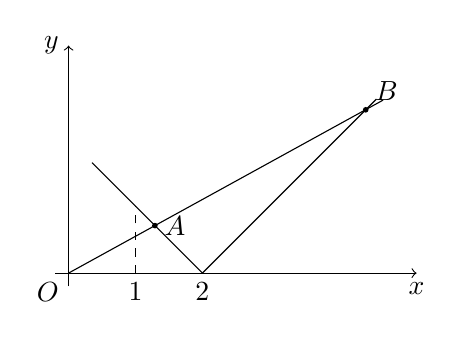
\begin{tikzpicture}[scale=0.85]
\draw[->] (-0.2,0) -- (5.2,0) node[below]{$x$};
\draw[->] (0,-0.2) -- (0,3.4) node[left]{$y$};
\node[below left] at (0,0) {$O$};
\draw (2,0) -- (0.35,1.65);
\draw (2,0) -- (4.6,2.6);
\draw (0,0) -- (4.7,2.585);
\draw[dashed] (1,0) -- (1,1);
\node[below] at (1,0) {$1$};
\node[below] at (2,0) {$2$};
\coordinate (A) at (1.29,0.71); \fill (A) circle (1.2pt); \node[right] at (A) {$A$};
\coordinate (B) at (4.44,2.44); \fill (B) circle (1.2pt); \node[above right] at (B) {$B$};
\end{tikzpicture}
\end{center}
\step{由 $0<k<1$，得 $x_A>1$，}
\step{所以关于 $x$ 的不等式 $k\lvert x\rvert-\lvert x-2\rvert>0$ 恰好有 $4$ 个整数解，是 $2,3,4,5$，}
\step{由 $\begin{cases}y=kx\\ y=x-2\end{cases}\Rightarrow x_B=\dfrac2{1-k}\in(5,6]$，故 $\dfrac35<k\leqslant\dfrac23$.}
\solend
\fi

\item 设集合 $S=\{1,2,3,\cdots,10\}$，$S$ 的子集 $A$ 满足 $A\cap\{1,2,3\}\neq\varnothing$，$A\cup\{4,5,6\}\neq S$，这样的子集 $A$ 的个数为\blankline[4.4em].

\ifanswer
\solbegin
\step{先求使 $A\cap\{1,2,3\}\neq\varnothing$ 成立的 $S$ 的子集 $A$ 的个数 $N_1$，}
\step{在 $\{1,2,3\}$ 中取出至少一个元素的方式有 $7$ 种，}
\step{而集合 $\{4,5,\cdots,10\}$ 的子集有 $2^7$ 个，因此 $N_1=7\times2^7=896$，}
% 注：下一行原卷印作“$A\cup\{4,5,6\}\neq S$”，按上下文应为“$=S$”，照录未改（见文件头“原卷笔误/存疑”①）。
\step{再扣除其中使 $A\cup\{4,5,6\}\neq S$ 的集合 $A$ 的个数 $N_2$，}
\step{这些取法中 $1$，$2$，$3$，$7$，$8$，$9$，$10$ 均被取出，}
\step{而集合 $\{4,5,6\}$ 的子集有 $2^3$ 个，因此 $N_2=2^3=8$，}
\step{从而满足条件的子集 $A$ 的个数为 $N_1-N_2=896-8=888$.}
\solend
\fi

\end{enumerate}

\bigsec{二、选择题}

\begin{enumerate}
\setcounter{enumi}{12}

\item 已知 $a>b$，下列不等式中一定成立是\mbox{（\quad）}

\keepwithprev
A. $a^2>b^2$\qquad B. $ac^2>bc^2$\qquad C. $\dfrac1a<\dfrac1b$\qquad D. $a+3>b-4$

\ifanswer
\solbegin
\step{对于 $A$，当 $a=-2$，$b=-4$ 时，不等式不成立，故 $A$ 错误；}
\step{对于 $B$，当 $c=0$ 时，不等式不成立，故 $B$ 错误；}
\step{对于 $C$，当 $a=2$，$b=-4$ 时，不等式不成立，故 $C$ 错误；}
\step{对于 $D$，因为 $a>b$，$3>-4$，必有 $a+3>b-4$ 成立，故 $D$ 正确.}
\solend
\fi

\item 已知集合 $M$ 满足 $\{2,3\}\subseteq M\subseteq\{1,2,3,4,5\}$，那么这样的集合 $M$ 的个数为\mbox{（\quad）}

\keepwithprev
A. $6$\qquad B. $7$\qquad C. $8$\qquad D. $9$

\ifanswer
\solbegin
\step{集合 $M$ 满足 $\{2,3\}\subseteq M\subseteq\{1,2,3,4,5\}$，所以 $2\in M$，$3\in M$，}
\step{故集合 $M$ 的个数为 $2^3=8$. 故选 $C$.}
\solend
\fi

\item 已知集合 $A=\{x\mid x=2k,k\in\Z\}$，$B=\{x\mid x=4m+6n,m,n\in\Z\}$，则\mbox{（\quad）}

\keepwithprev
A. $B\subset A$\qquad B. $A\subset B$\qquad C. $A=B$\qquad D. $B\neq A$

\ifanswer
\solbegin
\step{$B=\{x\mid x=4m+6n,m,n\in\Z\}$，$B$ 中的元素都是偶数，}
\step{所以 $B$ 的元素都是 $A$ 的元素，$B\subseteq A$；}
\step{$A=\{x\mid x=4(-k)+6k,k\in\Z\}$，则 $A$ 的元素都是 $B$ 的元素，$A\subseteq B$；}
\step{所以 $A=B$. 故选 $C$.}
\solend
\fi

\item 已知集合 $A=[1,a]\cup[a^3,a^4]$，集合 $B=\{x\mid x=x_1-x_2$，其中 $x_1,x_2\in A\}$. 若集合 $B$ 表示的区间为一个闭区间，则 $a$ 的取值范围为\mbox{（\quad）}

\keepwithprev
A. $a$ 取遍任意大于 $1$ 的实数\qquad B. $a\geqslant2$

C. $a\geqslant\dfrac{1+\sqrt5}2$\qquad D. $a\geqslant1+\sqrt2$

\ifanswer
\solbegin
\step{由题意得 $a^3>a>1$，则 $x_1-x_2$ 的最小值为 $1-a^4$，最大值为 $a^4-1$，}
\step{所以 $B=[1-a^4,a^4-1]$，}
\step{又因为 $a^4-a^3-(a-1)=a^3(a-1)-(a-1)=(a^3-1)(a-1)>0$，}
\step{所以 $a^4-a^3>a-1$，又集合 $B$ 表示的区间为一个闭区间，}
\step{则 $a^3-a\leqslant a^4-a^3$，化简得 $a^2-a-1\geqslant0$，又 $a>1$，解得 $a\geqslant\dfrac{1+\sqrt5}2$.}
\step{故选 $C$.}
\solend
\fi

\end{enumerate}

\bigsec{三、解答题}

\begin{enumerate}
\setcounter{enumi}{16}

\item 设全集 $U=\R$，集合 $A=\{x\mid\lvert x+3\rvert\leqslant4\}$，集合 $B=\{x\mid a-2\leqslant x\leqslant1+2a\}$，其中 $a\in\R$.

（1）若 $a=\dfrac12$，求 $A\cap B$；

（2）若 $A\cap B=\varnothing$，求 $a$ 的取值范围.

\ifanswer
\solbegin
\stepm{(1)}{由 $\lvert x+3\rvert\leqslant4$，得 $-4\leqslant x+3\leqslant4$，解得 $-7\leqslant x\leqslant1$，}
\step{所以 $A=\{x\mid-7\leqslant x\leqslant1\}$，}
\step{当 $a=\dfrac12$ 时，$a-2=\dfrac12-2=-\dfrac32$，$1+2a=1+2\times\dfrac12=2$，}
\step{$B=\left\{x\mid-\dfrac32\leqslant x\leqslant2\right\}$，$A\cap B=\left\{x\mid-\dfrac32\leqslant x\leqslant1\right\}$，即 $\left[-\dfrac32,1\right]$.}
\stepm{(2)}{若 $A\cap B=\varnothing$，分两种情况讨论，}
\step{①当 $B\neq\varnothing$ 时，$a-2\leqslant1+2a$，即 $a\geqslant-3$，}
\step{要满足 $A\cap B=\varnothing$，则 $1+2a<-7$ 或 $a-2>1$，}
\step{由 $1+2a<-7$，得 $a<-4$，与 $a\geqslant-3$ 无交集，无解，}
\step{由 $a-2>1$ 得 $a>3$，符合 $a\geqslant-3$，}
\step{②当 $B=\varnothing$ 时，有 $a-2>1+2a$，解得 $a<-3$，满足 $A\cap B=\varnothing$；}
\step{综上，$a$ 的取值范围是 $(-\infty,-3)\cup(3,+\infty)$.}
\solend
\fi

\ansspace

\item （1）已知 $a>b>0$，比较 $\dfrac{a+b}{a^2+b^2}$ 与 $\dfrac1{a-b}$ 的大小并说明理由；

（2）已知 $-2\leqslant x\leqslant-1$，$2\leqslant y\leqslant3$，求 $2x-y$ 的取值范围.

\ifanswer
\solbegin
\stepm{(1)}{$\dfrac{a+b}{a^2+b^2}-\dfrac1{a-b}=\dfrac{(a^2-b^2)-(a^2+b^2)}{(a^2+b^2)(a-b)}=\dfrac{-2b^2}{(a^2+b^2)(a-b)}$，}
\step{因为 $a>b>0$，所以 $a^2(a-b)-b^2(b-a)=(a^2+b^2)(a-b)>0$，}
\step{$\dfrac{-2b^2}{(a^2+b^2)(a-b)}<0$，即 $\dfrac{a+b}{a^2+b^2}-\dfrac1{a-b}<0$，所以 $\dfrac{a+b}{a^2+b^2}<\dfrac1{a-b}$；}
\stepm{(2)}{由 $-2\leqslant x\leqslant-1$，$2\leqslant y\leqslant3$，得 $-4\leqslant2x\leqslant-2$，$-3\leqslant-y\leqslant-2$，}
\step{得 $-7\leqslant2x-y\leqslant-4$，即 $2x-y$ 的取值范围为 $[-7,-4]$.}
\solend
\fi

\ansspace

\item 设 $x_1$、$x_2$ 是关于 $x$ 的方程 $x^2-2(m+2)x+m^2-1=0$ 的两个实数根.

（1）若 $\dfrac1{x_1}+\dfrac1{x_2}=-4$，求 $m$ 的值；

（2）若 $x_1$、$x_2$ 是两个不相等的正数，求实数 $m$ 的取值范围.

\ifanswer
\solbegin
\stepm{(1)}{因为 $x_1$、$x_2$ 是关于 $x$ 的方程的两个实数根，}
\step{所以 $\Delta=(-2(m+2))^2-4(m^2-1)=16m+20\geqslant0$，解得 $m\geqslant-\dfrac54$，}
\step{由韦达定理得 $x_1+x_2=2(m+2)$，$x_1x_2=m^2-1$，}
\step{所以 $\dfrac1{x_1}+\dfrac1{x_2}=\dfrac{x_2+x_1}{x_1x_2}=\dfrac{2(m+2)}{m^2-1}=-4$，即 $2m^2+m=0$，}
\step{解得 $m=0$ 或 $m=-\dfrac12$；}
\stepm{(2)}{由题意得 $\begin{cases}x_1+x_2>0\\ x_1x_2>0\\ \Delta>0\end{cases}$，即 $\begin{cases}2(m+2)>0\\ m^2-1>0\\ (-2(m+2))^2-4(m^2-1)>0\end{cases}$，}
\step{解得 $-\dfrac54<m<-1$ 或 $m>1$.}
\solend
\fi

\ansspace

\ifanswer\else\needvspace{10\baselineskip}\fi
\item 已知集合 $A=\{x\mid x\leqslant2\text{ 或 }x\geqslant a\}$.

（1）若 $B=\left\{x\mid(x-2)\left(x-\dfrac{12}{7-a}\right)<0\right\}$，$A\cap B=\varnothing$，$A\cup B=\R$，求实数 $a$ 的值；

（2）若 $a=3$ 且 $b<2$，$B=\{x\mid x^2-b(b+1)x+b^3<0\}$，$A\cap B\cap\Z$ 的子集个数为 $4$ 个，求实数 $b$ 的取值范围.

\ifanswer
\solbegin
\stepm{(1)}{当 $a\leqslant2$ 时，$A=\{x\mid x\leqslant2\text{ 或 }x\geqslant a\}=\R$，必有 $B=\varnothing$，}
\step{即不等式 $(x-2)\left(x-\dfrac{12}{7-a}\right)<0$ 无解，}
\step{必有 $\dfrac{12}{7-a}=2$，解得 $a=1$，符合题意，}
\step{当 $a>2$ 时，$A=(-\infty,2]\cup[a,+\infty)$，}
\step{若 $A\cap B=\varnothing$，$A\cup B=\R$，则 $B=(2,a)$，}
\step{即方程 $(x-2)\left(x-\dfrac{12}{7-a}\right)=0$ 的两个根是 $2$ 和 $a$，所以 $\dfrac{12}{7-a}=a$，}
\step{解得 $a=3$ 或 $a=4$，符合题意，}
\step{综上，实数 $a$ 的值为 $1$ 或 $3$ 或 $4$；}
\stepm{(2)}{由 $A\cap B\cap\Z$ 的子集个数为 $4$ 个，即 $A\cap B\cap\Z$ 中恰好有 $2$ 个整数元素，}
\step{由 $a=3$，则 $A=(-\infty,2]\cup[3,+\infty)$，}
\step{由 $x^2-b(b+1)x+b^3=(x-b^2)(x-b)<0$，又 $b<2$，}
\step{当 $1<b<2$ 时，$1<b^2<4$ 且 $b^2>b$，则 $B=(b,b^2)$，}
\step{则 $A\cap B=(b,2]\cup[3,b^2)$，}
\step{要使 $A\cap B\cap\Z$ 中恰好有 $2$ 个整数元素，即 $A\cap B\cap\Z=\{2,3\}$，}
\step{即 $\begin{cases}1<b<2\\ 3<b^2<4\end{cases}$，解得 $\sqrt3<b<2$，符合题意，}
\step{当 $b=1$ 或 $b=0$ 时，$B=\varnothing$，此时 $A\cap B\cap\Z=\varnothing$，不符合题意，舍去，}
\step{当 $0<b<1$ 时，$0<b^2<1$ 且 $b^2<b$，则 $B=(b^2,b)$，}
\step{此时 $A\cap B\cap\Z=\varnothing$，不符合题意，舍去，}
\step{当 $-1<b<0$ 时，$0<b^2<1$ 且 $b^2>b$，则 $B=(b,b^2)$，}
\step{此时 $A\cap B\cap\Z=\{0\}$，即 $A\cap B\cap\Z$ 中只有 $1$ 个元素，不符合题意，舍去，}
\step{当 $b\leqslant-1$ 时，$b^2\geqslant1$ 且 $b^2>b$，则 $B=(b,b^2)$，}
\step{此时 $A\cap B\cap\Z\supseteq\{-1,0,1\}$，即 $A\cap B\cap\Z$ 中至少有 $3$ 个元素，}
\step{不符合题意，舍去，}
\step{综上，实数 $b$ 的取值范围为 $(\sqrt3,2)$.}
\solend
\fi

\ansspace*[7]

\item 已知集合 $A=\{a_1,a_2,a_3,\cdots,a_n\}$ 中的元素均为正整数，其中 $n\in\N$ 且 $n\geqslant3$. 若对任意 $x,y\in A(x\neq y)$，都有 $\lvert x-y\rvert\geqslant\dfrac{xy}k$，则称集合 $A$ 具有性质 $M_k$.

（1）集合 $A=\{1,2,a\}$ 具有性质 $M_3$，求 $a$ 的最小值；

（2）若集合 $A$ 具有性质 $M_{24}$，且 $A$ 中最小元素和最大元素分别为 $a,b$，求证：$\dfrac1a-\dfrac1b\geqslant\dfrac{n-1}{24}$；

（3）已知集合 $A$ 具有性质 $M_{24}$，求 $A$ 中元素个数的最大值，并说明理由.

\ifanswer
\solbegin
\stepm{(1)}{由性质 $M_3$ 定义得 $\begin{cases}a-1\geqslant\dfrac a3\\ a-2\geqslant\dfrac{2a}3\end{cases}\Rightarrow\begin{cases}a\geqslant\dfrac32\\ a\geqslant6\end{cases}\Rightarrow a\geqslant6$，且 $a\subseteq\N^*$，}
% 注：上一行原卷印作“$a\subseteq\N^*$”，应为“$a\in\N^*$”，照录未改（见文件头“原卷笔误/存疑”②）。
\step{所以 $a$ 的最小值为 $6$.}
\stepm{(2)}{由题意得 $\lvert a_i-a_{i+1}\rvert\geqslant\dfrac{a_ia_{i+1}}{24}$，$(i=1,2,3,\cdots,n-1)$，且 $a_1<\cdots<a_n$，}
\step{所以 $a_{i+1}-a_i\geqslant\dfrac{a_ia_{i+1}}{24}\Rightarrow\dfrac1{a_i}-\dfrac1{a_{i+1}}\geqslant\dfrac1{24}$，$(i=1,2,3,\cdots,n-1)$，}
\step{所以 $\dfrac1{a_1}-\dfrac1{a_2}+\dfrac1{a_2}-\dfrac1{a_3}+\cdots+\dfrac1{a_{n-1}}-\dfrac1{a_n}=\dfrac1{a_1}-\dfrac1{a_n}\geqslant\dfrac{n-1}{24}$，得证.}
\stepm{(3)}{由 (2) 得 $\begin{cases}\dfrac1{a_1}\geqslant\dfrac{n-1}{24}\\ a_1\geqslant1\end{cases}\Rightarrow\dfrac{n-1}{24}<1\Rightarrow n<25$，}
\step{同 (2) 证明得 $\dfrac1{a_i}-\dfrac1{a_n}\geqslant\dfrac{n-i}{24}$ 且 $i=1,2,3,\cdots,n-1$，故 $\dfrac1{a_i}>\dfrac{n-i}{24}$，}
\step{又 $a_i\geqslant i$，所以 $\dfrac1i>\dfrac{n-i}{24}\Rightarrow i(n-i)<24$ 在 $i=1,2,3,\cdots,n-1$ 上恒成立，}
\step{当 $n\geqslant10$，取 $i=5$，则 $i(n-i)=5(n-5)>24$，故 $n<10$，}
\step{当 $n\leqslant9$，则 $i(n-i)\leqslant\dfrac{(i+n-i)^2}4=\dfrac{n^2}4<24\Rightarrow n<\sqrt{96}$，即 $n\leqslant9$.}
\step{综上，集合 $A$ 中元素个数的最大值为 $9$.}
\solend
\fi

\end{enumerate}

\end{document}
"
% 紧凑版：xelatex "\def\iscompact{1}% 高一79_南汇中学_10月月考.tex
%   —— 高一上数学“2026-2027 年南汇中学高一上 10 月月考”（讲评版）
% 试卷版：xelatex 高一79_南汇中学_10月月考.tex
% 答案版：xelatex "\def\isanswer{1}% 高一79_南汇中学_10月月考.tex
%   —— 高一上数学“2026-2027 年南汇中学高一上 10 月月考”（讲评版）
% 试卷版：xelatex 高一79_南汇中学_10月月考.tex
% 答案版：xelatex "\def\isanswer{1}\input{高一79_南汇中学_10月月考.tex}"
% 紧凑版：xelatex "\def\iscompact{1}\input{高一79_南汇中学_10月月考.tex}"
%
% 原始材料：微信公众号“魔都数学加油站”文章，连载“27学年高一79”；
% 原文标题“27学年高一79——2026-2027年上海市南汇中学高一上10月月考”；
% 原文链接：https://mp.weixin.qq.com/s/bFvc7GVgPTaDGg_6JSSfGg。
% 页面标注发布时间 2026-10-24 21:00（上海）。
% 正文为 9 张 PNG 页（`原图/高一79_南汇中学_10月月考/01..09.png`），
% 尺寸混排（第 1、2、4、5、7、8 页为 4762×6735，第 3、6、9 页为 2560×3620），均按页序读取。
%
% 篇幅与题号：原卷自第 3 题起编号。填空题 3—12（10 题）、选择题 13—16（4 题）、
% 解答题 17—21（5 题），共 19 题。
%
% 讲评版：第 4 题只印【答案】，本稿只给 \ans{}；其余 18 题印【解析】。
% 选择题答案在解析末句“故选 D／C／C／C”。
%
% 副标题：原卷未印副标题。本稿按内容标作“集合与常用逻辑用语、不等式”。
%
% 原卷笔误/存疑（均照录未改，正文对应处另有 % 注）：
%   ① 第 12 题解析作“再扣除其中使 $A\cup\{4,5,6\}\neq S$ 的集合 $A$ 的个数 $N_2$”，
%      按上下文应为“$A\cup\{4,5,6\}=S$”，否则“这些取法中 $1,2,3,7,8,9,10$ 均被取出”
%      与 $N_2=2^3=8$ 都无法解释；原卷印作 $\neq$，照录未改。
%   ② 第 21 题 (1) 解析末作“且 $a\subseteq\N^*$”，$a$ 是集合的元素，应为 $a\in\N^*$；
%      原卷印作 $\subseteq$，照录未改。
%
% 与原卷的排版差异：
%   ① 原卷每题下直接印【答案】/【解析】，本稿按全稿惯例将答案与解析置于答案版；
%   ② 原卷未印副标题，本稿补出；填空横线统一排 \blankline[4.4em]；
%   ③ 原卷数集记号排斜体 $R$、$Z$、$N$，本稿按全稿惯例改用 $\R$、$\Z$、$\N$；
%   ④ 第 17—21 题的子问用行内“（1）（2）（3）”段，解析中的子问标号用 \stepm；
%   ⑤ 解答题按惯例加 \ansspace；选择题括号排 \mbox{（\quad）}；
%   ⑥ 第 11 题解析有一幅函数图象（$y=k\lvert x\rvert$ 与 $y=\lvert x-2\rvert$），
%      按原图形状用 TikZ 重排（仅答案版出）。
%
% 行数核对：逐题数 \step/\stepm 条数，合计 107 条（Q3：2；Q5：2；Q6：1；Q7：4；Q8：4；
% Q9：4；Q10：5；Q11：4；Q12：7；Q13：4；Q14：2；Q15：4；Q16：6；Q17：11；Q18：5；
% Q19：7；Q20：24；Q21：11）。原卷解析的换行按语意合并，未逐行强拆；第 4 题只印
% 【答案】，提 \ans{}，不计入 \step 账。
%
\documentclass[a4paper,11pt]{article}
\usepackage{common}

\begin{document}

\examtitlest[3]{2026--2027 年南汇中学高一上 10 月月考}{集合与常用逻辑用语、不等式}

\bigsec{一、填空题}

\begin{enumerate}
\setcounter{enumi}{2}

\item 不等式 $\dfrac{1-x}{x}>0$ 的解集为\blankline[4.4em].

\ifanswer
\solbegin
\step{原不等式化为 $x(x-1)<0$，转化为 $\begin{cases}x>0\\ x-1<0\end{cases}$ 或 $\begin{cases}x<0\\ x-1>0\end{cases}$，}
\step{解得 $0<x<1$，则不等式的解集为 $\{x\mid0<x<1\}$.}
\solend
\fi

\item 用反证法证明命题：“若 $x^2<1$，则 $-1<x<1$”时，应假设\blankline[4.4em].

\ifanswer
\ans{$x\geqslant1$ 或 $x\leqslant-1$}
\fi

\item 设 $k$ 为实数，关于 $x$ 的不等式 $kx^2+x+2<0$ 的解集为 $A$，若 $2\notin A$，则 $k$ 的取值范围是\blankline[4.4em].

\ifanswer
\solbegin
\step{因为关于 $x$ 的不等式 $kx^2+x+2<0$ 的解集为 $A$，且 $2\notin A$，}
\step{所以 $x=2$ 时，$k\times2^2+2+2\geqslant0$，解得 $k\geqslant-1$，则 $k$ 的取值范围为 $[-1,+\infty)$.}
\solend
\fi

\item 已知集合 $M=\{y\mid y=x^2-2x,x\in\R\}$，$N=\{x\mid y=\sqrt{4-x^2}\}$，则 $M\cup N=$\blankline[4.4em].

\ifanswer
\solbegin
\step{$M=[-1,+\infty)$，$N=[-2,2]$，则 $M\cup N=[-2,+\infty)$.}
\solend
\fi

\item 设集合 $A=\{-3,2\}$，集合 $B=\{x\mid mx+1=0\}$，且 $A\cup B=A$，则 $m$ 的值组成的集合是\blankline[4.4em].

\ifanswer
\solbegin
\step{由 $A\cup B=A$，得 $B\subseteq A$，}
\step{当 $m=0$ 时，$B=\varnothing$，满足题意，}
\step{当 $m\neq0$ 时，$B=\left\{-\dfrac1m\right\}$，所以 $-\dfrac1m=2$ 或 $-\dfrac1m=-3$，所以 $m=-\dfrac12$ 或 $m=\dfrac13$，}
\step{综上所述，$m$ 的值组成的集合是 $\left\{0,-\dfrac12,\dfrac13\right\}$.}
\solend
\fi

\item 若不等式 $\lvert x\rvert<a$ 的一个充分不必要条件为 $\dfrac{2x-1}{x-2}<1$，则实数 $a$ 的取值范围是\blankline[4.4em].

\ifanswer
\solbegin
\step{不等式 $\lvert x\rvert<a$，得 $-a<x<a$，}
\step{不等式 $\dfrac{2x-1}{x-2}<1$，即 $\dfrac{2x-1-(x-2)}{x-2}=\dfrac{x+1}{x-2}<0$，解得 $-1<x<2$，}
\step{又不等式 $\lvert x\rvert<a$ 的一个充分不必要条件为 $\dfrac{2x-1}{x-2}<1$，}
\step{得 $\begin{cases}a\geqslant2\\ -a\leqslant-1\end{cases}$，且两等号不同时成立，解得 $a\geqslant2$.}
\solend
\fi

\item 若对任意 $x\in\R$ 都有 $(m-1)x^2-(m-1)x-1<0$，则实数 $m$ 的取值范围是\blankline[4.4em].

\ifanswer
\solbegin
\step{当 $m-1\neq0$，即 $m\neq1$ 时，则有 $\begin{cases}m-1<0\\ (m-1)^2-4(m-1)\times(-1)<0\end{cases}$，}
\step{解得 $-3<m<1$；}
\step{当 $m-1=0$ 时，即当 $m=1$ 时，此时不等式为 $-1<0$ 恒成立，符合题意；}
\step{综上所述，实数 $m$ 的取值范围是 $(-3,1]$.}
\solend
\fi

\item 关于 $x$ 的方程 $\dfrac{x}{x-1}=\dfrac{k-x}{x^2-x}$ 的解集中只含有一个元素，则 $k$ 的可能取值构成的集合为\blankline[4.4em].

\ifanswer
\solbegin
\step{方程两边同时乘以 $x(x-1)$ 得 $x^2=k-x$，即 $x^2+x-k=0$，}
\step{①当其中一个解为增根时，方程也只有一个解，}
\step{(i) 若增根为 $0$ 时，$k=0$；(ii) 若增根为 $1$ 时，$k=2$；}
\step{②当 $\Delta=1+4k=0$，即 $k=-\dfrac14$ 时，方程 $x^2+x-k=0$ 只有一个解；}
\step{即 $k$ 的可能取值构成的集合为 $\left\{-\dfrac14,0,2\right\}$.}
\solend
\fi

\item 若关于 $x$ 的不等式 $k\lvert x\rvert>\lvert x-2\rvert$ 恰好有 $4$ 个整数解，则实数 $k$ 的取值范围是\blankline[4.4em].

\ifanswer
\solbegin
\step{由题意得 $0<k<1$，函数 $y=k\lvert x\rvert$ 与 $y=\lvert x-2\rvert$ 的图象如图：}
\begin{center}
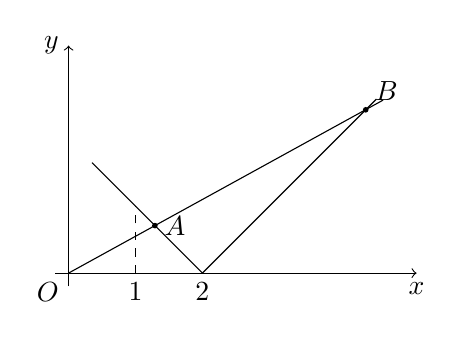
\begin{tikzpicture}[scale=0.85]
\draw[->] (-0.2,0) -- (5.2,0) node[below]{$x$};
\draw[->] (0,-0.2) -- (0,3.4) node[left]{$y$};
\node[below left] at (0,0) {$O$};
\draw (2,0) -- (0.35,1.65);
\draw (2,0) -- (4.6,2.6);
\draw (0,0) -- (4.7,2.585);
\draw[dashed] (1,0) -- (1,1);
\node[below] at (1,0) {$1$};
\node[below] at (2,0) {$2$};
\coordinate (A) at (1.29,0.71); \fill (A) circle (1.2pt); \node[right] at (A) {$A$};
\coordinate (B) at (4.44,2.44); \fill (B) circle (1.2pt); \node[above right] at (B) {$B$};
\end{tikzpicture}
\end{center}
\step{由 $0<k<1$，得 $x_A>1$，}
\step{所以关于 $x$ 的不等式 $k\lvert x\rvert-\lvert x-2\rvert>0$ 恰好有 $4$ 个整数解，是 $2,3,4,5$，}
\step{由 $\begin{cases}y=kx\\ y=x-2\end{cases}\Rightarrow x_B=\dfrac2{1-k}\in(5,6]$，故 $\dfrac35<k\leqslant\dfrac23$.}
\solend
\fi

\item 设集合 $S=\{1,2,3,\cdots,10\}$，$S$ 的子集 $A$ 满足 $A\cap\{1,2,3\}\neq\varnothing$，$A\cup\{4,5,6\}\neq S$，这样的子集 $A$ 的个数为\blankline[4.4em].

\ifanswer
\solbegin
\step{先求使 $A\cap\{1,2,3\}\neq\varnothing$ 成立的 $S$ 的子集 $A$ 的个数 $N_1$，}
\step{在 $\{1,2,3\}$ 中取出至少一个元素的方式有 $7$ 种，}
\step{而集合 $\{4,5,\cdots,10\}$ 的子集有 $2^7$ 个，因此 $N_1=7\times2^7=896$，}
% 注：下一行原卷印作“$A\cup\{4,5,6\}\neq S$”，按上下文应为“$=S$”，照录未改（见文件头“原卷笔误/存疑”①）。
\step{再扣除其中使 $A\cup\{4,5,6\}\neq S$ 的集合 $A$ 的个数 $N_2$，}
\step{这些取法中 $1$，$2$，$3$，$7$，$8$，$9$，$10$ 均被取出，}
\step{而集合 $\{4,5,6\}$ 的子集有 $2^3$ 个，因此 $N_2=2^3=8$，}
\step{从而满足条件的子集 $A$ 的个数为 $N_1-N_2=896-8=888$.}
\solend
\fi

\end{enumerate}

\bigsec{二、选择题}

\begin{enumerate}
\setcounter{enumi}{12}

\item 已知 $a>b$，下列不等式中一定成立是\mbox{（\quad）}

\keepwithprev
A. $a^2>b^2$\qquad B. $ac^2>bc^2$\qquad C. $\dfrac1a<\dfrac1b$\qquad D. $a+3>b-4$

\ifanswer
\solbegin
\step{对于 $A$，当 $a=-2$，$b=-4$ 时，不等式不成立，故 $A$ 错误；}
\step{对于 $B$，当 $c=0$ 时，不等式不成立，故 $B$ 错误；}
\step{对于 $C$，当 $a=2$，$b=-4$ 时，不等式不成立，故 $C$ 错误；}
\step{对于 $D$，因为 $a>b$，$3>-4$，必有 $a+3>b-4$ 成立，故 $D$ 正确.}
\solend
\fi

\item 已知集合 $M$ 满足 $\{2,3\}\subseteq M\subseteq\{1,2,3,4,5\}$，那么这样的集合 $M$ 的个数为\mbox{（\quad）}

\keepwithprev
A. $6$\qquad B. $7$\qquad C. $8$\qquad D. $9$

\ifanswer
\solbegin
\step{集合 $M$ 满足 $\{2,3\}\subseteq M\subseteq\{1,2,3,4,5\}$，所以 $2\in M$，$3\in M$，}
\step{故集合 $M$ 的个数为 $2^3=8$. 故选 $C$.}
\solend
\fi

\item 已知集合 $A=\{x\mid x=2k,k\in\Z\}$，$B=\{x\mid x=4m+6n,m,n\in\Z\}$，则\mbox{（\quad）}

\keepwithprev
A. $B\subset A$\qquad B. $A\subset B$\qquad C. $A=B$\qquad D. $B\neq A$

\ifanswer
\solbegin
\step{$B=\{x\mid x=4m+6n,m,n\in\Z\}$，$B$ 中的元素都是偶数，}
\step{所以 $B$ 的元素都是 $A$ 的元素，$B\subseteq A$；}
\step{$A=\{x\mid x=4(-k)+6k,k\in\Z\}$，则 $A$ 的元素都是 $B$ 的元素，$A\subseteq B$；}
\step{所以 $A=B$. 故选 $C$.}
\solend
\fi

\item 已知集合 $A=[1,a]\cup[a^3,a^4]$，集合 $B=\{x\mid x=x_1-x_2$，其中 $x_1,x_2\in A\}$. 若集合 $B$ 表示的区间为一个闭区间，则 $a$ 的取值范围为\mbox{（\quad）}

\keepwithprev
A. $a$ 取遍任意大于 $1$ 的实数\qquad B. $a\geqslant2$

C. $a\geqslant\dfrac{1+\sqrt5}2$\qquad D. $a\geqslant1+\sqrt2$

\ifanswer
\solbegin
\step{由题意得 $a^3>a>1$，则 $x_1-x_2$ 的最小值为 $1-a^4$，最大值为 $a^4-1$，}
\step{所以 $B=[1-a^4,a^4-1]$，}
\step{又因为 $a^4-a^3-(a-1)=a^3(a-1)-(a-1)=(a^3-1)(a-1)>0$，}
\step{所以 $a^4-a^3>a-1$，又集合 $B$ 表示的区间为一个闭区间，}
\step{则 $a^3-a\leqslant a^4-a^3$，化简得 $a^2-a-1\geqslant0$，又 $a>1$，解得 $a\geqslant\dfrac{1+\sqrt5}2$.}
\step{故选 $C$.}
\solend
\fi

\end{enumerate}

\bigsec{三、解答题}

\begin{enumerate}
\setcounter{enumi}{16}

\item 设全集 $U=\R$，集合 $A=\{x\mid\lvert x+3\rvert\leqslant4\}$，集合 $B=\{x\mid a-2\leqslant x\leqslant1+2a\}$，其中 $a\in\R$.

（1）若 $a=\dfrac12$，求 $A\cap B$；

（2）若 $A\cap B=\varnothing$，求 $a$ 的取值范围.

\ifanswer
\solbegin
\stepm{(1)}{由 $\lvert x+3\rvert\leqslant4$，得 $-4\leqslant x+3\leqslant4$，解得 $-7\leqslant x\leqslant1$，}
\step{所以 $A=\{x\mid-7\leqslant x\leqslant1\}$，}
\step{当 $a=\dfrac12$ 时，$a-2=\dfrac12-2=-\dfrac32$，$1+2a=1+2\times\dfrac12=2$，}
\step{$B=\left\{x\mid-\dfrac32\leqslant x\leqslant2\right\}$，$A\cap B=\left\{x\mid-\dfrac32\leqslant x\leqslant1\right\}$，即 $\left[-\dfrac32,1\right]$.}
\stepm{(2)}{若 $A\cap B=\varnothing$，分两种情况讨论，}
\step{①当 $B\neq\varnothing$ 时，$a-2\leqslant1+2a$，即 $a\geqslant-3$，}
\step{要满足 $A\cap B=\varnothing$，则 $1+2a<-7$ 或 $a-2>1$，}
\step{由 $1+2a<-7$，得 $a<-4$，与 $a\geqslant-3$ 无交集，无解，}
\step{由 $a-2>1$ 得 $a>3$，符合 $a\geqslant-3$，}
\step{②当 $B=\varnothing$ 时，有 $a-2>1+2a$，解得 $a<-3$，满足 $A\cap B=\varnothing$；}
\step{综上，$a$ 的取值范围是 $(-\infty,-3)\cup(3,+\infty)$.}
\solend
\fi

\ansspace

\item （1）已知 $a>b>0$，比较 $\dfrac{a+b}{a^2+b^2}$ 与 $\dfrac1{a-b}$ 的大小并说明理由；

（2）已知 $-2\leqslant x\leqslant-1$，$2\leqslant y\leqslant3$，求 $2x-y$ 的取值范围.

\ifanswer
\solbegin
\stepm{(1)}{$\dfrac{a+b}{a^2+b^2}-\dfrac1{a-b}=\dfrac{(a^2-b^2)-(a^2+b^2)}{(a^2+b^2)(a-b)}=\dfrac{-2b^2}{(a^2+b^2)(a-b)}$，}
\step{因为 $a>b>0$，所以 $a^2(a-b)-b^2(b-a)=(a^2+b^2)(a-b)>0$，}
\step{$\dfrac{-2b^2}{(a^2+b^2)(a-b)}<0$，即 $\dfrac{a+b}{a^2+b^2}-\dfrac1{a-b}<0$，所以 $\dfrac{a+b}{a^2+b^2}<\dfrac1{a-b}$；}
\stepm{(2)}{由 $-2\leqslant x\leqslant-1$，$2\leqslant y\leqslant3$，得 $-4\leqslant2x\leqslant-2$，$-3\leqslant-y\leqslant-2$，}
\step{得 $-7\leqslant2x-y\leqslant-4$，即 $2x-y$ 的取值范围为 $[-7,-4]$.}
\solend
\fi

\ansspace

\item 设 $x_1$、$x_2$ 是关于 $x$ 的方程 $x^2-2(m+2)x+m^2-1=0$ 的两个实数根.

（1）若 $\dfrac1{x_1}+\dfrac1{x_2}=-4$，求 $m$ 的值；

（2）若 $x_1$、$x_2$ 是两个不相等的正数，求实数 $m$ 的取值范围.

\ifanswer
\solbegin
\stepm{(1)}{因为 $x_1$、$x_2$ 是关于 $x$ 的方程的两个实数根，}
\step{所以 $\Delta=(-2(m+2))^2-4(m^2-1)=16m+20\geqslant0$，解得 $m\geqslant-\dfrac54$，}
\step{由韦达定理得 $x_1+x_2=2(m+2)$，$x_1x_2=m^2-1$，}
\step{所以 $\dfrac1{x_1}+\dfrac1{x_2}=\dfrac{x_2+x_1}{x_1x_2}=\dfrac{2(m+2)}{m^2-1}=-4$，即 $2m^2+m=0$，}
\step{解得 $m=0$ 或 $m=-\dfrac12$；}
\stepm{(2)}{由题意得 $\begin{cases}x_1+x_2>0\\ x_1x_2>0\\ \Delta>0\end{cases}$，即 $\begin{cases}2(m+2)>0\\ m^2-1>0\\ (-2(m+2))^2-4(m^2-1)>0\end{cases}$，}
\step{解得 $-\dfrac54<m<-1$ 或 $m>1$.}
\solend
\fi

\ansspace

\ifanswer\else\needvspace{10\baselineskip}\fi
\item 已知集合 $A=\{x\mid x\leqslant2\text{ 或 }x\geqslant a\}$.

（1）若 $B=\left\{x\mid(x-2)\left(x-\dfrac{12}{7-a}\right)<0\right\}$，$A\cap B=\varnothing$，$A\cup B=\R$，求实数 $a$ 的值；

（2）若 $a=3$ 且 $b<2$，$B=\{x\mid x^2-b(b+1)x+b^3<0\}$，$A\cap B\cap\Z$ 的子集个数为 $4$ 个，求实数 $b$ 的取值范围.

\ifanswer
\solbegin
\stepm{(1)}{当 $a\leqslant2$ 时，$A=\{x\mid x\leqslant2\text{ 或 }x\geqslant a\}=\R$，必有 $B=\varnothing$，}
\step{即不等式 $(x-2)\left(x-\dfrac{12}{7-a}\right)<0$ 无解，}
\step{必有 $\dfrac{12}{7-a}=2$，解得 $a=1$，符合题意，}
\step{当 $a>2$ 时，$A=(-\infty,2]\cup[a,+\infty)$，}
\step{若 $A\cap B=\varnothing$，$A\cup B=\R$，则 $B=(2,a)$，}
\step{即方程 $(x-2)\left(x-\dfrac{12}{7-a}\right)=0$ 的两个根是 $2$ 和 $a$，所以 $\dfrac{12}{7-a}=a$，}
\step{解得 $a=3$ 或 $a=4$，符合题意，}
\step{综上，实数 $a$ 的值为 $1$ 或 $3$ 或 $4$；}
\stepm{(2)}{由 $A\cap B\cap\Z$ 的子集个数为 $4$ 个，即 $A\cap B\cap\Z$ 中恰好有 $2$ 个整数元素，}
\step{由 $a=3$，则 $A=(-\infty,2]\cup[3,+\infty)$，}
\step{由 $x^2-b(b+1)x+b^3=(x-b^2)(x-b)<0$，又 $b<2$，}
\step{当 $1<b<2$ 时，$1<b^2<4$ 且 $b^2>b$，则 $B=(b,b^2)$，}
\step{则 $A\cap B=(b,2]\cup[3,b^2)$，}
\step{要使 $A\cap B\cap\Z$ 中恰好有 $2$ 个整数元素，即 $A\cap B\cap\Z=\{2,3\}$，}
\step{即 $\begin{cases}1<b<2\\ 3<b^2<4\end{cases}$，解得 $\sqrt3<b<2$，符合题意，}
\step{当 $b=1$ 或 $b=0$ 时，$B=\varnothing$，此时 $A\cap B\cap\Z=\varnothing$，不符合题意，舍去，}
\step{当 $0<b<1$ 时，$0<b^2<1$ 且 $b^2<b$，则 $B=(b^2,b)$，}
\step{此时 $A\cap B\cap\Z=\varnothing$，不符合题意，舍去，}
\step{当 $-1<b<0$ 时，$0<b^2<1$ 且 $b^2>b$，则 $B=(b,b^2)$，}
\step{此时 $A\cap B\cap\Z=\{0\}$，即 $A\cap B\cap\Z$ 中只有 $1$ 个元素，不符合题意，舍去，}
\step{当 $b\leqslant-1$ 时，$b^2\geqslant1$ 且 $b^2>b$，则 $B=(b,b^2)$，}
\step{此时 $A\cap B\cap\Z\supseteq\{-1,0,1\}$，即 $A\cap B\cap\Z$ 中至少有 $3$ 个元素，}
\step{不符合题意，舍去，}
\step{综上，实数 $b$ 的取值范围为 $(\sqrt3,2)$.}
\solend
\fi

\ansspace*[7]

\item 已知集合 $A=\{a_1,a_2,a_3,\cdots,a_n\}$ 中的元素均为正整数，其中 $n\in\N$ 且 $n\geqslant3$. 若对任意 $x,y\in A(x\neq y)$，都有 $\lvert x-y\rvert\geqslant\dfrac{xy}k$，则称集合 $A$ 具有性质 $M_k$.

（1）集合 $A=\{1,2,a\}$ 具有性质 $M_3$，求 $a$ 的最小值；

（2）若集合 $A$ 具有性质 $M_{24}$，且 $A$ 中最小元素和最大元素分别为 $a,b$，求证：$\dfrac1a-\dfrac1b\geqslant\dfrac{n-1}{24}$；

（3）已知集合 $A$ 具有性质 $M_{24}$，求 $A$ 中元素个数的最大值，并说明理由.

\ifanswer
\solbegin
\stepm{(1)}{由性质 $M_3$ 定义得 $\begin{cases}a-1\geqslant\dfrac a3\\ a-2\geqslant\dfrac{2a}3\end{cases}\Rightarrow\begin{cases}a\geqslant\dfrac32\\ a\geqslant6\end{cases}\Rightarrow a\geqslant6$，且 $a\subseteq\N^*$，}
% 注：上一行原卷印作“$a\subseteq\N^*$”，应为“$a\in\N^*$”，照录未改（见文件头“原卷笔误/存疑”②）。
\step{所以 $a$ 的最小值为 $6$.}
\stepm{(2)}{由题意得 $\lvert a_i-a_{i+1}\rvert\geqslant\dfrac{a_ia_{i+1}}{24}$，$(i=1,2,3,\cdots,n-1)$，且 $a_1<\cdots<a_n$，}
\step{所以 $a_{i+1}-a_i\geqslant\dfrac{a_ia_{i+1}}{24}\Rightarrow\dfrac1{a_i}-\dfrac1{a_{i+1}}\geqslant\dfrac1{24}$，$(i=1,2,3,\cdots,n-1)$，}
\step{所以 $\dfrac1{a_1}-\dfrac1{a_2}+\dfrac1{a_2}-\dfrac1{a_3}+\cdots+\dfrac1{a_{n-1}}-\dfrac1{a_n}=\dfrac1{a_1}-\dfrac1{a_n}\geqslant\dfrac{n-1}{24}$，得证.}
\stepm{(3)}{由 (2) 得 $\begin{cases}\dfrac1{a_1}\geqslant\dfrac{n-1}{24}\\ a_1\geqslant1\end{cases}\Rightarrow\dfrac{n-1}{24}<1\Rightarrow n<25$，}
\step{同 (2) 证明得 $\dfrac1{a_i}-\dfrac1{a_n}\geqslant\dfrac{n-i}{24}$ 且 $i=1,2,3,\cdots,n-1$，故 $\dfrac1{a_i}>\dfrac{n-i}{24}$，}
\step{又 $a_i\geqslant i$，所以 $\dfrac1i>\dfrac{n-i}{24}\Rightarrow i(n-i)<24$ 在 $i=1,2,3,\cdots,n-1$ 上恒成立，}
\step{当 $n\geqslant10$，取 $i=5$，则 $i(n-i)=5(n-5)>24$，故 $n<10$，}
\step{当 $n\leqslant9$，则 $i(n-i)\leqslant\dfrac{(i+n-i)^2}4=\dfrac{n^2}4<24\Rightarrow n<\sqrt{96}$，即 $n\leqslant9$.}
\step{综上，集合 $A$ 中元素个数的最大值为 $9$.}
\solend
\fi

\end{enumerate}

\end{document}
"
% 紧凑版：xelatex "\def\iscompact{1}% 高一79_南汇中学_10月月考.tex
%   —— 高一上数学“2026-2027 年南汇中学高一上 10 月月考”（讲评版）
% 试卷版：xelatex 高一79_南汇中学_10月月考.tex
% 答案版：xelatex "\def\isanswer{1}\input{高一79_南汇中学_10月月考.tex}"
% 紧凑版：xelatex "\def\iscompact{1}\input{高一79_南汇中学_10月月考.tex}"
%
% 原始材料：微信公众号“魔都数学加油站”文章，连载“27学年高一79”；
% 原文标题“27学年高一79——2026-2027年上海市南汇中学高一上10月月考”；
% 原文链接：https://mp.weixin.qq.com/s/bFvc7GVgPTaDGg_6JSSfGg。
% 页面标注发布时间 2026-10-24 21:00（上海）。
% 正文为 9 张 PNG 页（`原图/高一79_南汇中学_10月月考/01..09.png`），
% 尺寸混排（第 1、2、4、5、7、8 页为 4762×6735，第 3、6、9 页为 2560×3620），均按页序读取。
%
% 篇幅与题号：原卷自第 3 题起编号。填空题 3—12（10 题）、选择题 13—16（4 题）、
% 解答题 17—21（5 题），共 19 题。
%
% 讲评版：第 4 题只印【答案】，本稿只给 \ans{}；其余 18 题印【解析】。
% 选择题答案在解析末句“故选 D／C／C／C”。
%
% 副标题：原卷未印副标题。本稿按内容标作“集合与常用逻辑用语、不等式”。
%
% 原卷笔误/存疑（均照录未改，正文对应处另有 % 注）：
%   ① 第 12 题解析作“再扣除其中使 $A\cup\{4,5,6\}\neq S$ 的集合 $A$ 的个数 $N_2$”，
%      按上下文应为“$A\cup\{4,5,6\}=S$”，否则“这些取法中 $1,2,3,7,8,9,10$ 均被取出”
%      与 $N_2=2^3=8$ 都无法解释；原卷印作 $\neq$，照录未改。
%   ② 第 21 题 (1) 解析末作“且 $a\subseteq\N^*$”，$a$ 是集合的元素，应为 $a\in\N^*$；
%      原卷印作 $\subseteq$，照录未改。
%
% 与原卷的排版差异：
%   ① 原卷每题下直接印【答案】/【解析】，本稿按全稿惯例将答案与解析置于答案版；
%   ② 原卷未印副标题，本稿补出；填空横线统一排 \blankline[4.4em]；
%   ③ 原卷数集记号排斜体 $R$、$Z$、$N$，本稿按全稿惯例改用 $\R$、$\Z$、$\N$；
%   ④ 第 17—21 题的子问用行内“（1）（2）（3）”段，解析中的子问标号用 \stepm；
%   ⑤ 解答题按惯例加 \ansspace；选择题括号排 \mbox{（\quad）}；
%   ⑥ 第 11 题解析有一幅函数图象（$y=k\lvert x\rvert$ 与 $y=\lvert x-2\rvert$），
%      按原图形状用 TikZ 重排（仅答案版出）。
%
% 行数核对：逐题数 \step/\stepm 条数，合计 107 条（Q3：2；Q5：2；Q6：1；Q7：4；Q8：4；
% Q9：4；Q10：5；Q11：4；Q12：7；Q13：4；Q14：2；Q15：4；Q16：6；Q17：11；Q18：5；
% Q19：7；Q20：24；Q21：11）。原卷解析的换行按语意合并，未逐行强拆；第 4 题只印
% 【答案】，提 \ans{}，不计入 \step 账。
%
\documentclass[a4paper,11pt]{article}
\usepackage{common}

\begin{document}

\examtitlest[3]{2026--2027 年南汇中学高一上 10 月月考}{集合与常用逻辑用语、不等式}

\bigsec{一、填空题}

\begin{enumerate}
\setcounter{enumi}{2}

\item 不等式 $\dfrac{1-x}{x}>0$ 的解集为\blankline[4.4em].

\ifanswer
\solbegin
\step{原不等式化为 $x(x-1)<0$，转化为 $\begin{cases}x>0\\ x-1<0\end{cases}$ 或 $\begin{cases}x<0\\ x-1>0\end{cases}$，}
\step{解得 $0<x<1$，则不等式的解集为 $\{x\mid0<x<1\}$.}
\solend
\fi

\item 用反证法证明命题：“若 $x^2<1$，则 $-1<x<1$”时，应假设\blankline[4.4em].

\ifanswer
\ans{$x\geqslant1$ 或 $x\leqslant-1$}
\fi

\item 设 $k$ 为实数，关于 $x$ 的不等式 $kx^2+x+2<0$ 的解集为 $A$，若 $2\notin A$，则 $k$ 的取值范围是\blankline[4.4em].

\ifanswer
\solbegin
\step{因为关于 $x$ 的不等式 $kx^2+x+2<0$ 的解集为 $A$，且 $2\notin A$，}
\step{所以 $x=2$ 时，$k\times2^2+2+2\geqslant0$，解得 $k\geqslant-1$，则 $k$ 的取值范围为 $[-1,+\infty)$.}
\solend
\fi

\item 已知集合 $M=\{y\mid y=x^2-2x,x\in\R\}$，$N=\{x\mid y=\sqrt{4-x^2}\}$，则 $M\cup N=$\blankline[4.4em].

\ifanswer
\solbegin
\step{$M=[-1,+\infty)$，$N=[-2,2]$，则 $M\cup N=[-2,+\infty)$.}
\solend
\fi

\item 设集合 $A=\{-3,2\}$，集合 $B=\{x\mid mx+1=0\}$，且 $A\cup B=A$，则 $m$ 的值组成的集合是\blankline[4.4em].

\ifanswer
\solbegin
\step{由 $A\cup B=A$，得 $B\subseteq A$，}
\step{当 $m=0$ 时，$B=\varnothing$，满足题意，}
\step{当 $m\neq0$ 时，$B=\left\{-\dfrac1m\right\}$，所以 $-\dfrac1m=2$ 或 $-\dfrac1m=-3$，所以 $m=-\dfrac12$ 或 $m=\dfrac13$，}
\step{综上所述，$m$ 的值组成的集合是 $\left\{0,-\dfrac12,\dfrac13\right\}$.}
\solend
\fi

\item 若不等式 $\lvert x\rvert<a$ 的一个充分不必要条件为 $\dfrac{2x-1}{x-2}<1$，则实数 $a$ 的取值范围是\blankline[4.4em].

\ifanswer
\solbegin
\step{不等式 $\lvert x\rvert<a$，得 $-a<x<a$，}
\step{不等式 $\dfrac{2x-1}{x-2}<1$，即 $\dfrac{2x-1-(x-2)}{x-2}=\dfrac{x+1}{x-2}<0$，解得 $-1<x<2$，}
\step{又不等式 $\lvert x\rvert<a$ 的一个充分不必要条件为 $\dfrac{2x-1}{x-2}<1$，}
\step{得 $\begin{cases}a\geqslant2\\ -a\leqslant-1\end{cases}$，且两等号不同时成立，解得 $a\geqslant2$.}
\solend
\fi

\item 若对任意 $x\in\R$ 都有 $(m-1)x^2-(m-1)x-1<0$，则实数 $m$ 的取值范围是\blankline[4.4em].

\ifanswer
\solbegin
\step{当 $m-1\neq0$，即 $m\neq1$ 时，则有 $\begin{cases}m-1<0\\ (m-1)^2-4(m-1)\times(-1)<0\end{cases}$，}
\step{解得 $-3<m<1$；}
\step{当 $m-1=0$ 时，即当 $m=1$ 时，此时不等式为 $-1<0$ 恒成立，符合题意；}
\step{综上所述，实数 $m$ 的取值范围是 $(-3,1]$.}
\solend
\fi

\item 关于 $x$ 的方程 $\dfrac{x}{x-1}=\dfrac{k-x}{x^2-x}$ 的解集中只含有一个元素，则 $k$ 的可能取值构成的集合为\blankline[4.4em].

\ifanswer
\solbegin
\step{方程两边同时乘以 $x(x-1)$ 得 $x^2=k-x$，即 $x^2+x-k=0$，}
\step{①当其中一个解为增根时，方程也只有一个解，}
\step{(i) 若增根为 $0$ 时，$k=0$；(ii) 若增根为 $1$ 时，$k=2$；}
\step{②当 $\Delta=1+4k=0$，即 $k=-\dfrac14$ 时，方程 $x^2+x-k=0$ 只有一个解；}
\step{即 $k$ 的可能取值构成的集合为 $\left\{-\dfrac14,0,2\right\}$.}
\solend
\fi

\item 若关于 $x$ 的不等式 $k\lvert x\rvert>\lvert x-2\rvert$ 恰好有 $4$ 个整数解，则实数 $k$ 的取值范围是\blankline[4.4em].

\ifanswer
\solbegin
\step{由题意得 $0<k<1$，函数 $y=k\lvert x\rvert$ 与 $y=\lvert x-2\rvert$ 的图象如图：}
\begin{center}
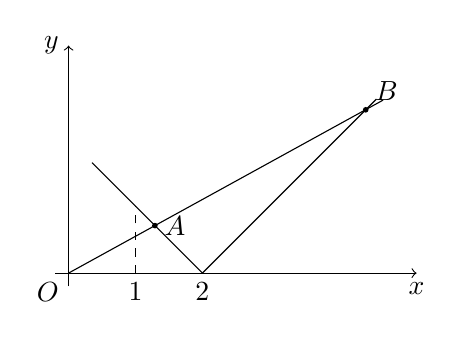
\begin{tikzpicture}[scale=0.85]
\draw[->] (-0.2,0) -- (5.2,0) node[below]{$x$};
\draw[->] (0,-0.2) -- (0,3.4) node[left]{$y$};
\node[below left] at (0,0) {$O$};
\draw (2,0) -- (0.35,1.65);
\draw (2,0) -- (4.6,2.6);
\draw (0,0) -- (4.7,2.585);
\draw[dashed] (1,0) -- (1,1);
\node[below] at (1,0) {$1$};
\node[below] at (2,0) {$2$};
\coordinate (A) at (1.29,0.71); \fill (A) circle (1.2pt); \node[right] at (A) {$A$};
\coordinate (B) at (4.44,2.44); \fill (B) circle (1.2pt); \node[above right] at (B) {$B$};
\end{tikzpicture}
\end{center}
\step{由 $0<k<1$，得 $x_A>1$，}
\step{所以关于 $x$ 的不等式 $k\lvert x\rvert-\lvert x-2\rvert>0$ 恰好有 $4$ 个整数解，是 $2,3,4,5$，}
\step{由 $\begin{cases}y=kx\\ y=x-2\end{cases}\Rightarrow x_B=\dfrac2{1-k}\in(5,6]$，故 $\dfrac35<k\leqslant\dfrac23$.}
\solend
\fi

\item 设集合 $S=\{1,2,3,\cdots,10\}$，$S$ 的子集 $A$ 满足 $A\cap\{1,2,3\}\neq\varnothing$，$A\cup\{4,5,6\}\neq S$，这样的子集 $A$ 的个数为\blankline[4.4em].

\ifanswer
\solbegin
\step{先求使 $A\cap\{1,2,3\}\neq\varnothing$ 成立的 $S$ 的子集 $A$ 的个数 $N_1$，}
\step{在 $\{1,2,3\}$ 中取出至少一个元素的方式有 $7$ 种，}
\step{而集合 $\{4,5,\cdots,10\}$ 的子集有 $2^7$ 个，因此 $N_1=7\times2^7=896$，}
% 注：下一行原卷印作“$A\cup\{4,5,6\}\neq S$”，按上下文应为“$=S$”，照录未改（见文件头“原卷笔误/存疑”①）。
\step{再扣除其中使 $A\cup\{4,5,6\}\neq S$ 的集合 $A$ 的个数 $N_2$，}
\step{这些取法中 $1$，$2$，$3$，$7$，$8$，$9$，$10$ 均被取出，}
\step{而集合 $\{4,5,6\}$ 的子集有 $2^3$ 个，因此 $N_2=2^3=8$，}
\step{从而满足条件的子集 $A$ 的个数为 $N_1-N_2=896-8=888$.}
\solend
\fi

\end{enumerate}

\bigsec{二、选择题}

\begin{enumerate}
\setcounter{enumi}{12}

\item 已知 $a>b$，下列不等式中一定成立是\mbox{（\quad）}

\keepwithprev
A. $a^2>b^2$\qquad B. $ac^2>bc^2$\qquad C. $\dfrac1a<\dfrac1b$\qquad D. $a+3>b-4$

\ifanswer
\solbegin
\step{对于 $A$，当 $a=-2$，$b=-4$ 时，不等式不成立，故 $A$ 错误；}
\step{对于 $B$，当 $c=0$ 时，不等式不成立，故 $B$ 错误；}
\step{对于 $C$，当 $a=2$，$b=-4$ 时，不等式不成立，故 $C$ 错误；}
\step{对于 $D$，因为 $a>b$，$3>-4$，必有 $a+3>b-4$ 成立，故 $D$ 正确.}
\solend
\fi

\item 已知集合 $M$ 满足 $\{2,3\}\subseteq M\subseteq\{1,2,3,4,5\}$，那么这样的集合 $M$ 的个数为\mbox{（\quad）}

\keepwithprev
A. $6$\qquad B. $7$\qquad C. $8$\qquad D. $9$

\ifanswer
\solbegin
\step{集合 $M$ 满足 $\{2,3\}\subseteq M\subseteq\{1,2,3,4,5\}$，所以 $2\in M$，$3\in M$，}
\step{故集合 $M$ 的个数为 $2^3=8$. 故选 $C$.}
\solend
\fi

\item 已知集合 $A=\{x\mid x=2k,k\in\Z\}$，$B=\{x\mid x=4m+6n,m,n\in\Z\}$，则\mbox{（\quad）}

\keepwithprev
A. $B\subset A$\qquad B. $A\subset B$\qquad C. $A=B$\qquad D. $B\neq A$

\ifanswer
\solbegin
\step{$B=\{x\mid x=4m+6n,m,n\in\Z\}$，$B$ 中的元素都是偶数，}
\step{所以 $B$ 的元素都是 $A$ 的元素，$B\subseteq A$；}
\step{$A=\{x\mid x=4(-k)+6k,k\in\Z\}$，则 $A$ 的元素都是 $B$ 的元素，$A\subseteq B$；}
\step{所以 $A=B$. 故选 $C$.}
\solend
\fi

\item 已知集合 $A=[1,a]\cup[a^3,a^4]$，集合 $B=\{x\mid x=x_1-x_2$，其中 $x_1,x_2\in A\}$. 若集合 $B$ 表示的区间为一个闭区间，则 $a$ 的取值范围为\mbox{（\quad）}

\keepwithprev
A. $a$ 取遍任意大于 $1$ 的实数\qquad B. $a\geqslant2$

C. $a\geqslant\dfrac{1+\sqrt5}2$\qquad D. $a\geqslant1+\sqrt2$

\ifanswer
\solbegin
\step{由题意得 $a^3>a>1$，则 $x_1-x_2$ 的最小值为 $1-a^4$，最大值为 $a^4-1$，}
\step{所以 $B=[1-a^4,a^4-1]$，}
\step{又因为 $a^4-a^3-(a-1)=a^3(a-1)-(a-1)=(a^3-1)(a-1)>0$，}
\step{所以 $a^4-a^3>a-1$，又集合 $B$ 表示的区间为一个闭区间，}
\step{则 $a^3-a\leqslant a^4-a^3$，化简得 $a^2-a-1\geqslant0$，又 $a>1$，解得 $a\geqslant\dfrac{1+\sqrt5}2$.}
\step{故选 $C$.}
\solend
\fi

\end{enumerate}

\bigsec{三、解答题}

\begin{enumerate}
\setcounter{enumi}{16}

\item 设全集 $U=\R$，集合 $A=\{x\mid\lvert x+3\rvert\leqslant4\}$，集合 $B=\{x\mid a-2\leqslant x\leqslant1+2a\}$，其中 $a\in\R$.

（1）若 $a=\dfrac12$，求 $A\cap B$；

（2）若 $A\cap B=\varnothing$，求 $a$ 的取值范围.

\ifanswer
\solbegin
\stepm{(1)}{由 $\lvert x+3\rvert\leqslant4$，得 $-4\leqslant x+3\leqslant4$，解得 $-7\leqslant x\leqslant1$，}
\step{所以 $A=\{x\mid-7\leqslant x\leqslant1\}$，}
\step{当 $a=\dfrac12$ 时，$a-2=\dfrac12-2=-\dfrac32$，$1+2a=1+2\times\dfrac12=2$，}
\step{$B=\left\{x\mid-\dfrac32\leqslant x\leqslant2\right\}$，$A\cap B=\left\{x\mid-\dfrac32\leqslant x\leqslant1\right\}$，即 $\left[-\dfrac32,1\right]$.}
\stepm{(2)}{若 $A\cap B=\varnothing$，分两种情况讨论，}
\step{①当 $B\neq\varnothing$ 时，$a-2\leqslant1+2a$，即 $a\geqslant-3$，}
\step{要满足 $A\cap B=\varnothing$，则 $1+2a<-7$ 或 $a-2>1$，}
\step{由 $1+2a<-7$，得 $a<-4$，与 $a\geqslant-3$ 无交集，无解，}
\step{由 $a-2>1$ 得 $a>3$，符合 $a\geqslant-3$，}
\step{②当 $B=\varnothing$ 时，有 $a-2>1+2a$，解得 $a<-3$，满足 $A\cap B=\varnothing$；}
\step{综上，$a$ 的取值范围是 $(-\infty,-3)\cup(3,+\infty)$.}
\solend
\fi

\ansspace

\item （1）已知 $a>b>0$，比较 $\dfrac{a+b}{a^2+b^2}$ 与 $\dfrac1{a-b}$ 的大小并说明理由；

（2）已知 $-2\leqslant x\leqslant-1$，$2\leqslant y\leqslant3$，求 $2x-y$ 的取值范围.

\ifanswer
\solbegin
\stepm{(1)}{$\dfrac{a+b}{a^2+b^2}-\dfrac1{a-b}=\dfrac{(a^2-b^2)-(a^2+b^2)}{(a^2+b^2)(a-b)}=\dfrac{-2b^2}{(a^2+b^2)(a-b)}$，}
\step{因为 $a>b>0$，所以 $a^2(a-b)-b^2(b-a)=(a^2+b^2)(a-b)>0$，}
\step{$\dfrac{-2b^2}{(a^2+b^2)(a-b)}<0$，即 $\dfrac{a+b}{a^2+b^2}-\dfrac1{a-b}<0$，所以 $\dfrac{a+b}{a^2+b^2}<\dfrac1{a-b}$；}
\stepm{(2)}{由 $-2\leqslant x\leqslant-1$，$2\leqslant y\leqslant3$，得 $-4\leqslant2x\leqslant-2$，$-3\leqslant-y\leqslant-2$，}
\step{得 $-7\leqslant2x-y\leqslant-4$，即 $2x-y$ 的取值范围为 $[-7,-4]$.}
\solend
\fi

\ansspace

\item 设 $x_1$、$x_2$ 是关于 $x$ 的方程 $x^2-2(m+2)x+m^2-1=0$ 的两个实数根.

（1）若 $\dfrac1{x_1}+\dfrac1{x_2}=-4$，求 $m$ 的值；

（2）若 $x_1$、$x_2$ 是两个不相等的正数，求实数 $m$ 的取值范围.

\ifanswer
\solbegin
\stepm{(1)}{因为 $x_1$、$x_2$ 是关于 $x$ 的方程的两个实数根，}
\step{所以 $\Delta=(-2(m+2))^2-4(m^2-1)=16m+20\geqslant0$，解得 $m\geqslant-\dfrac54$，}
\step{由韦达定理得 $x_1+x_2=2(m+2)$，$x_1x_2=m^2-1$，}
\step{所以 $\dfrac1{x_1}+\dfrac1{x_2}=\dfrac{x_2+x_1}{x_1x_2}=\dfrac{2(m+2)}{m^2-1}=-4$，即 $2m^2+m=0$，}
\step{解得 $m=0$ 或 $m=-\dfrac12$；}
\stepm{(2)}{由题意得 $\begin{cases}x_1+x_2>0\\ x_1x_2>0\\ \Delta>0\end{cases}$，即 $\begin{cases}2(m+2)>0\\ m^2-1>0\\ (-2(m+2))^2-4(m^2-1)>0\end{cases}$，}
\step{解得 $-\dfrac54<m<-1$ 或 $m>1$.}
\solend
\fi

\ansspace

\ifanswer\else\needvspace{10\baselineskip}\fi
\item 已知集合 $A=\{x\mid x\leqslant2\text{ 或 }x\geqslant a\}$.

（1）若 $B=\left\{x\mid(x-2)\left(x-\dfrac{12}{7-a}\right)<0\right\}$，$A\cap B=\varnothing$，$A\cup B=\R$，求实数 $a$ 的值；

（2）若 $a=3$ 且 $b<2$，$B=\{x\mid x^2-b(b+1)x+b^3<0\}$，$A\cap B\cap\Z$ 的子集个数为 $4$ 个，求实数 $b$ 的取值范围.

\ifanswer
\solbegin
\stepm{(1)}{当 $a\leqslant2$ 时，$A=\{x\mid x\leqslant2\text{ 或 }x\geqslant a\}=\R$，必有 $B=\varnothing$，}
\step{即不等式 $(x-2)\left(x-\dfrac{12}{7-a}\right)<0$ 无解，}
\step{必有 $\dfrac{12}{7-a}=2$，解得 $a=1$，符合题意，}
\step{当 $a>2$ 时，$A=(-\infty,2]\cup[a,+\infty)$，}
\step{若 $A\cap B=\varnothing$，$A\cup B=\R$，则 $B=(2,a)$，}
\step{即方程 $(x-2)\left(x-\dfrac{12}{7-a}\right)=0$ 的两个根是 $2$ 和 $a$，所以 $\dfrac{12}{7-a}=a$，}
\step{解得 $a=3$ 或 $a=4$，符合题意，}
\step{综上，实数 $a$ 的值为 $1$ 或 $3$ 或 $4$；}
\stepm{(2)}{由 $A\cap B\cap\Z$ 的子集个数为 $4$ 个，即 $A\cap B\cap\Z$ 中恰好有 $2$ 个整数元素，}
\step{由 $a=3$，则 $A=(-\infty,2]\cup[3,+\infty)$，}
\step{由 $x^2-b(b+1)x+b^3=(x-b^2)(x-b)<0$，又 $b<2$，}
\step{当 $1<b<2$ 时，$1<b^2<4$ 且 $b^2>b$，则 $B=(b,b^2)$，}
\step{则 $A\cap B=(b,2]\cup[3,b^2)$，}
\step{要使 $A\cap B\cap\Z$ 中恰好有 $2$ 个整数元素，即 $A\cap B\cap\Z=\{2,3\}$，}
\step{即 $\begin{cases}1<b<2\\ 3<b^2<4\end{cases}$，解得 $\sqrt3<b<2$，符合题意，}
\step{当 $b=1$ 或 $b=0$ 时，$B=\varnothing$，此时 $A\cap B\cap\Z=\varnothing$，不符合题意，舍去，}
\step{当 $0<b<1$ 时，$0<b^2<1$ 且 $b^2<b$，则 $B=(b^2,b)$，}
\step{此时 $A\cap B\cap\Z=\varnothing$，不符合题意，舍去，}
\step{当 $-1<b<0$ 时，$0<b^2<1$ 且 $b^2>b$，则 $B=(b,b^2)$，}
\step{此时 $A\cap B\cap\Z=\{0\}$，即 $A\cap B\cap\Z$ 中只有 $1$ 个元素，不符合题意，舍去，}
\step{当 $b\leqslant-1$ 时，$b^2\geqslant1$ 且 $b^2>b$，则 $B=(b,b^2)$，}
\step{此时 $A\cap B\cap\Z\supseteq\{-1,0,1\}$，即 $A\cap B\cap\Z$ 中至少有 $3$ 个元素，}
\step{不符合题意，舍去，}
\step{综上，实数 $b$ 的取值范围为 $(\sqrt3,2)$.}
\solend
\fi

\ansspace*[7]

\item 已知集合 $A=\{a_1,a_2,a_3,\cdots,a_n\}$ 中的元素均为正整数，其中 $n\in\N$ 且 $n\geqslant3$. 若对任意 $x,y\in A(x\neq y)$，都有 $\lvert x-y\rvert\geqslant\dfrac{xy}k$，则称集合 $A$ 具有性质 $M_k$.

（1）集合 $A=\{1,2,a\}$ 具有性质 $M_3$，求 $a$ 的最小值；

（2）若集合 $A$ 具有性质 $M_{24}$，且 $A$ 中最小元素和最大元素分别为 $a,b$，求证：$\dfrac1a-\dfrac1b\geqslant\dfrac{n-1}{24}$；

（3）已知集合 $A$ 具有性质 $M_{24}$，求 $A$ 中元素个数的最大值，并说明理由.

\ifanswer
\solbegin
\stepm{(1)}{由性质 $M_3$ 定义得 $\begin{cases}a-1\geqslant\dfrac a3\\ a-2\geqslant\dfrac{2a}3\end{cases}\Rightarrow\begin{cases}a\geqslant\dfrac32\\ a\geqslant6\end{cases}\Rightarrow a\geqslant6$，且 $a\subseteq\N^*$，}
% 注：上一行原卷印作“$a\subseteq\N^*$”，应为“$a\in\N^*$”，照录未改（见文件头“原卷笔误/存疑”②）。
\step{所以 $a$ 的最小值为 $6$.}
\stepm{(2)}{由题意得 $\lvert a_i-a_{i+1}\rvert\geqslant\dfrac{a_ia_{i+1}}{24}$，$(i=1,2,3,\cdots,n-1)$，且 $a_1<\cdots<a_n$，}
\step{所以 $a_{i+1}-a_i\geqslant\dfrac{a_ia_{i+1}}{24}\Rightarrow\dfrac1{a_i}-\dfrac1{a_{i+1}}\geqslant\dfrac1{24}$，$(i=1,2,3,\cdots,n-1)$，}
\step{所以 $\dfrac1{a_1}-\dfrac1{a_2}+\dfrac1{a_2}-\dfrac1{a_3}+\cdots+\dfrac1{a_{n-1}}-\dfrac1{a_n}=\dfrac1{a_1}-\dfrac1{a_n}\geqslant\dfrac{n-1}{24}$，得证.}
\stepm{(3)}{由 (2) 得 $\begin{cases}\dfrac1{a_1}\geqslant\dfrac{n-1}{24}\\ a_1\geqslant1\end{cases}\Rightarrow\dfrac{n-1}{24}<1\Rightarrow n<25$，}
\step{同 (2) 证明得 $\dfrac1{a_i}-\dfrac1{a_n}\geqslant\dfrac{n-i}{24}$ 且 $i=1,2,3,\cdots,n-1$，故 $\dfrac1{a_i}>\dfrac{n-i}{24}$，}
\step{又 $a_i\geqslant i$，所以 $\dfrac1i>\dfrac{n-i}{24}\Rightarrow i(n-i)<24$ 在 $i=1,2,3,\cdots,n-1$ 上恒成立，}
\step{当 $n\geqslant10$，取 $i=5$，则 $i(n-i)=5(n-5)>24$，故 $n<10$，}
\step{当 $n\leqslant9$，则 $i(n-i)\leqslant\dfrac{(i+n-i)^2}4=\dfrac{n^2}4<24\Rightarrow n<\sqrt{96}$，即 $n\leqslant9$.}
\step{综上，集合 $A$ 中元素个数的最大值为 $9$.}
\solend
\fi

\end{enumerate}

\end{document}
"
%
% 原始材料：微信公众号“魔都数学加油站”文章，连载“27学年高一79”；
% 原文标题“27学年高一79——2026-2027年上海市南汇中学高一上10月月考”；
% 原文链接：https://mp.weixin.qq.com/s/bFvc7GVgPTaDGg_6JSSfGg。
% 页面标注发布时间 2026-10-24 21:00（上海）。
% 正文为 9 张 PNG 页（`原图/高一79_南汇中学_10月月考/01..09.png`），
% 尺寸混排（第 1、2、4、5、7、8 页为 4762×6735，第 3、6、9 页为 2560×3620），均按页序读取。
%
% 篇幅与题号：原卷自第 3 题起编号。填空题 3—12（10 题）、选择题 13—16（4 题）、
% 解答题 17—21（5 题），共 19 题。
%
% 讲评版：第 4 题只印【答案】，本稿只给 \ans{}；其余 18 题印【解析】。
% 选择题答案在解析末句“故选 D／C／C／C”。
%
% 副标题：原卷未印副标题。本稿按内容标作“集合与常用逻辑用语、不等式”。
%
% 原卷笔误/存疑（均照录未改，正文对应处另有 % 注）：
%   ① 第 12 题解析作“再扣除其中使 $A\cup\{4,5,6\}\neq S$ 的集合 $A$ 的个数 $N_2$”，
%      按上下文应为“$A\cup\{4,5,6\}=S$”，否则“这些取法中 $1,2,3,7,8,9,10$ 均被取出”
%      与 $N_2=2^3=8$ 都无法解释；原卷印作 $\neq$，照录未改。
%   ② 第 21 题 (1) 解析末作“且 $a\subseteq\N^*$”，$a$ 是集合的元素，应为 $a\in\N^*$；
%      原卷印作 $\subseteq$，照录未改。
%
% 与原卷的排版差异：
%   ① 原卷每题下直接印【答案】/【解析】，本稿按全稿惯例将答案与解析置于答案版；
%   ② 原卷未印副标题，本稿补出；填空横线统一排 \blankline[4.4em]；
%   ③ 原卷数集记号排斜体 $R$、$Z$、$N$，本稿按全稿惯例改用 $\R$、$\Z$、$\N$；
%   ④ 第 17—21 题的子问用行内“（1）（2）（3）”段，解析中的子问标号用 \stepm；
%   ⑤ 解答题按惯例加 \ansspace；选择题括号排 \mbox{（\quad）}；
%   ⑥ 第 11 题解析有一幅函数图象（$y=k\lvert x\rvert$ 与 $y=\lvert x-2\rvert$），
%      按原图形状用 TikZ 重排（仅答案版出）。
%
% 行数核对：逐题数 \step/\stepm 条数，合计 107 条（Q3：2；Q5：2；Q6：1；Q7：4；Q8：4；
% Q9：4；Q10：5；Q11：4；Q12：7；Q13：4；Q14：2；Q15：4；Q16：6；Q17：11；Q18：5；
% Q19：7；Q20：24；Q21：11）。原卷解析的换行按语意合并，未逐行强拆；第 4 题只印
% 【答案】，提 \ans{}，不计入 \step 账。
%
\documentclass[a4paper,11pt]{article}
\usepackage{common}

\begin{document}

\examtitlest[3]{2026--2027 年南汇中学高一上 10 月月考}{集合与常用逻辑用语、不等式}

\bigsec{一、填空题}

\begin{enumerate}
\setcounter{enumi}{2}

\item 不等式 $\dfrac{1-x}{x}>0$ 的解集为\blankline[4.4em].

\ifanswer
\solbegin
\step{原不等式化为 $x(x-1)<0$，转化为 $\begin{cases}x>0\\ x-1<0\end{cases}$ 或 $\begin{cases}x<0\\ x-1>0\end{cases}$，}
\step{解得 $0<x<1$，则不等式的解集为 $\{x\mid0<x<1\}$.}
\solend
\fi

\item 用反证法证明命题：“若 $x^2<1$，则 $-1<x<1$”时，应假设\blankline[4.4em].

\ifanswer
\ans{$x\geqslant1$ 或 $x\leqslant-1$}
\fi

\item 设 $k$ 为实数，关于 $x$ 的不等式 $kx^2+x+2<0$ 的解集为 $A$，若 $2\notin A$，则 $k$ 的取值范围是\blankline[4.4em].

\ifanswer
\solbegin
\step{因为关于 $x$ 的不等式 $kx^2+x+2<0$ 的解集为 $A$，且 $2\notin A$，}
\step{所以 $x=2$ 时，$k\times2^2+2+2\geqslant0$，解得 $k\geqslant-1$，则 $k$ 的取值范围为 $[-1,+\infty)$.}
\solend
\fi

\item 已知集合 $M=\{y\mid y=x^2-2x,x\in\R\}$，$N=\{x\mid y=\sqrt{4-x^2}\}$，则 $M\cup N=$\blankline[4.4em].

\ifanswer
\solbegin
\step{$M=[-1,+\infty)$，$N=[-2,2]$，则 $M\cup N=[-2,+\infty)$.}
\solend
\fi

\item 设集合 $A=\{-3,2\}$，集合 $B=\{x\mid mx+1=0\}$，且 $A\cup B=A$，则 $m$ 的值组成的集合是\blankline[4.4em].

\ifanswer
\solbegin
\step{由 $A\cup B=A$，得 $B\subseteq A$，}
\step{当 $m=0$ 时，$B=\varnothing$，满足题意，}
\step{当 $m\neq0$ 时，$B=\left\{-\dfrac1m\right\}$，所以 $-\dfrac1m=2$ 或 $-\dfrac1m=-3$，所以 $m=-\dfrac12$ 或 $m=\dfrac13$，}
\step{综上所述，$m$ 的值组成的集合是 $\left\{0,-\dfrac12,\dfrac13\right\}$.}
\solend
\fi

\item 若不等式 $\lvert x\rvert<a$ 的一个充分不必要条件为 $\dfrac{2x-1}{x-2}<1$，则实数 $a$ 的取值范围是\blankline[4.4em].

\ifanswer
\solbegin
\step{不等式 $\lvert x\rvert<a$，得 $-a<x<a$，}
\step{不等式 $\dfrac{2x-1}{x-2}<1$，即 $\dfrac{2x-1-(x-2)}{x-2}=\dfrac{x+1}{x-2}<0$，解得 $-1<x<2$，}
\step{又不等式 $\lvert x\rvert<a$ 的一个充分不必要条件为 $\dfrac{2x-1}{x-2}<1$，}
\step{得 $\begin{cases}a\geqslant2\\ -a\leqslant-1\end{cases}$，且两等号不同时成立，解得 $a\geqslant2$.}
\solend
\fi

\item 若对任意 $x\in\R$ 都有 $(m-1)x^2-(m-1)x-1<0$，则实数 $m$ 的取值范围是\blankline[4.4em].

\ifanswer
\solbegin
\step{当 $m-1\neq0$，即 $m\neq1$ 时，则有 $\begin{cases}m-1<0\\ (m-1)^2-4(m-1)\times(-1)<0\end{cases}$，}
\step{解得 $-3<m<1$；}
\step{当 $m-1=0$ 时，即当 $m=1$ 时，此时不等式为 $-1<0$ 恒成立，符合题意；}
\step{综上所述，实数 $m$ 的取值范围是 $(-3,1]$.}
\solend
\fi

\item 关于 $x$ 的方程 $\dfrac{x}{x-1}=\dfrac{k-x}{x^2-x}$ 的解集中只含有一个元素，则 $k$ 的可能取值构成的集合为\blankline[4.4em].

\ifanswer
\solbegin
\step{方程两边同时乘以 $x(x-1)$ 得 $x^2=k-x$，即 $x^2+x-k=0$，}
\step{①当其中一个解为增根时，方程也只有一个解，}
\step{(i) 若增根为 $0$ 时，$k=0$；(ii) 若增根为 $1$ 时，$k=2$；}
\step{②当 $\Delta=1+4k=0$，即 $k=-\dfrac14$ 时，方程 $x^2+x-k=0$ 只有一个解；}
\step{即 $k$ 的可能取值构成的集合为 $\left\{-\dfrac14,0,2\right\}$.}
\solend
\fi

\item 若关于 $x$ 的不等式 $k\lvert x\rvert>\lvert x-2\rvert$ 恰好有 $4$ 个整数解，则实数 $k$ 的取值范围是\blankline[4.4em].

\ifanswer
\solbegin
\step{由题意得 $0<k<1$，函数 $y=k\lvert x\rvert$ 与 $y=\lvert x-2\rvert$ 的图象如图：}
\begin{center}
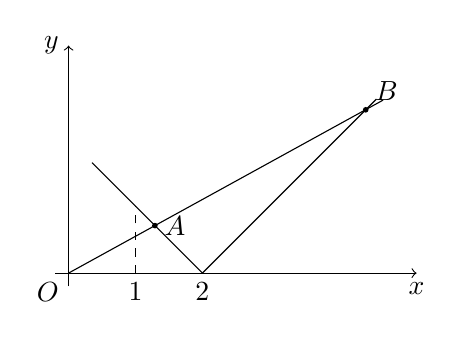
\begin{tikzpicture}[scale=0.85]
\draw[->] (-0.2,0) -- (5.2,0) node[below]{$x$};
\draw[->] (0,-0.2) -- (0,3.4) node[left]{$y$};
\node[below left] at (0,0) {$O$};
\draw (2,0) -- (0.35,1.65);
\draw (2,0) -- (4.6,2.6);
\draw (0,0) -- (4.7,2.585);
\draw[dashed] (1,0) -- (1,1);
\node[below] at (1,0) {$1$};
\node[below] at (2,0) {$2$};
\coordinate (A) at (1.29,0.71); \fill (A) circle (1.2pt); \node[right] at (A) {$A$};
\coordinate (B) at (4.44,2.44); \fill (B) circle (1.2pt); \node[above right] at (B) {$B$};
\end{tikzpicture}
\end{center}
\step{由 $0<k<1$，得 $x_A>1$，}
\step{所以关于 $x$ 的不等式 $k\lvert x\rvert-\lvert x-2\rvert>0$ 恰好有 $4$ 个整数解，是 $2,3,4,5$，}
\step{由 $\begin{cases}y=kx\\ y=x-2\end{cases}\Rightarrow x_B=\dfrac2{1-k}\in(5,6]$，故 $\dfrac35<k\leqslant\dfrac23$.}
\solend
\fi

\item 设集合 $S=\{1,2,3,\cdots,10\}$，$S$ 的子集 $A$ 满足 $A\cap\{1,2,3\}\neq\varnothing$，$A\cup\{4,5,6\}\neq S$，这样的子集 $A$ 的个数为\blankline[4.4em].

\ifanswer
\solbegin
\step{先求使 $A\cap\{1,2,3\}\neq\varnothing$ 成立的 $S$ 的子集 $A$ 的个数 $N_1$，}
\step{在 $\{1,2,3\}$ 中取出至少一个元素的方式有 $7$ 种，}
\step{而集合 $\{4,5,\cdots,10\}$ 的子集有 $2^7$ 个，因此 $N_1=7\times2^7=896$，}
% 注：下一行原卷印作“$A\cup\{4,5,6\}\neq S$”，按上下文应为“$=S$”，照录未改（见文件头“原卷笔误/存疑”①）。
\step{再扣除其中使 $A\cup\{4,5,6\}\neq S$ 的集合 $A$ 的个数 $N_2$，}
\step{这些取法中 $1$，$2$，$3$，$7$，$8$，$9$，$10$ 均被取出，}
\step{而集合 $\{4,5,6\}$ 的子集有 $2^3$ 个，因此 $N_2=2^3=8$，}
\step{从而满足条件的子集 $A$ 的个数为 $N_1-N_2=896-8=888$.}
\solend
\fi

\end{enumerate}

\bigsec{二、选择题}

\begin{enumerate}
\setcounter{enumi}{12}

\item 已知 $a>b$，下列不等式中一定成立是\mbox{（\quad）}

\keepwithprev
A. $a^2>b^2$\qquad B. $ac^2>bc^2$\qquad C. $\dfrac1a<\dfrac1b$\qquad D. $a+3>b-4$

\ifanswer
\solbegin
\step{对于 $A$，当 $a=-2$，$b=-4$ 时，不等式不成立，故 $A$ 错误；}
\step{对于 $B$，当 $c=0$ 时，不等式不成立，故 $B$ 错误；}
\step{对于 $C$，当 $a=2$，$b=-4$ 时，不等式不成立，故 $C$ 错误；}
\step{对于 $D$，因为 $a>b$，$3>-4$，必有 $a+3>b-4$ 成立，故 $D$ 正确.}
\solend
\fi

\item 已知集合 $M$ 满足 $\{2,3\}\subseteq M\subseteq\{1,2,3,4,5\}$，那么这样的集合 $M$ 的个数为\mbox{（\quad）}

\keepwithprev
A. $6$\qquad B. $7$\qquad C. $8$\qquad D. $9$

\ifanswer
\solbegin
\step{集合 $M$ 满足 $\{2,3\}\subseteq M\subseteq\{1,2,3,4,5\}$，所以 $2\in M$，$3\in M$，}
\step{故集合 $M$ 的个数为 $2^3=8$. 故选 $C$.}
\solend
\fi

\item 已知集合 $A=\{x\mid x=2k,k\in\Z\}$，$B=\{x\mid x=4m+6n,m,n\in\Z\}$，则\mbox{（\quad）}

\keepwithprev
A. $B\subset A$\qquad B. $A\subset B$\qquad C. $A=B$\qquad D. $B\neq A$

\ifanswer
\solbegin
\step{$B=\{x\mid x=4m+6n,m,n\in\Z\}$，$B$ 中的元素都是偶数，}
\step{所以 $B$ 的元素都是 $A$ 的元素，$B\subseteq A$；}
\step{$A=\{x\mid x=4(-k)+6k,k\in\Z\}$，则 $A$ 的元素都是 $B$ 的元素，$A\subseteq B$；}
\step{所以 $A=B$. 故选 $C$.}
\solend
\fi

\item 已知集合 $A=[1,a]\cup[a^3,a^4]$，集合 $B=\{x\mid x=x_1-x_2$，其中 $x_1,x_2\in A\}$. 若集合 $B$ 表示的区间为一个闭区间，则 $a$ 的取值范围为\mbox{（\quad）}

\keepwithprev
A. $a$ 取遍任意大于 $1$ 的实数\qquad B. $a\geqslant2$

C. $a\geqslant\dfrac{1+\sqrt5}2$\qquad D. $a\geqslant1+\sqrt2$

\ifanswer
\solbegin
\step{由题意得 $a^3>a>1$，则 $x_1-x_2$ 的最小值为 $1-a^4$，最大值为 $a^4-1$，}
\step{所以 $B=[1-a^4,a^4-1]$，}
\step{又因为 $a^4-a^3-(a-1)=a^3(a-1)-(a-1)=(a^3-1)(a-1)>0$，}
\step{所以 $a^4-a^3>a-1$，又集合 $B$ 表示的区间为一个闭区间，}
\step{则 $a^3-a\leqslant a^4-a^3$，化简得 $a^2-a-1\geqslant0$，又 $a>1$，解得 $a\geqslant\dfrac{1+\sqrt5}2$.}
\step{故选 $C$.}
\solend
\fi

\end{enumerate}

\bigsec{三、解答题}

\begin{enumerate}
\setcounter{enumi}{16}

\item 设全集 $U=\R$，集合 $A=\{x\mid\lvert x+3\rvert\leqslant4\}$，集合 $B=\{x\mid a-2\leqslant x\leqslant1+2a\}$，其中 $a\in\R$.

（1）若 $a=\dfrac12$，求 $A\cap B$；

（2）若 $A\cap B=\varnothing$，求 $a$ 的取值范围.

\ifanswer
\solbegin
\stepm{(1)}{由 $\lvert x+3\rvert\leqslant4$，得 $-4\leqslant x+3\leqslant4$，解得 $-7\leqslant x\leqslant1$，}
\step{所以 $A=\{x\mid-7\leqslant x\leqslant1\}$，}
\step{当 $a=\dfrac12$ 时，$a-2=\dfrac12-2=-\dfrac32$，$1+2a=1+2\times\dfrac12=2$，}
\step{$B=\left\{x\mid-\dfrac32\leqslant x\leqslant2\right\}$，$A\cap B=\left\{x\mid-\dfrac32\leqslant x\leqslant1\right\}$，即 $\left[-\dfrac32,1\right]$.}
\stepm{(2)}{若 $A\cap B=\varnothing$，分两种情况讨论，}
\step{①当 $B\neq\varnothing$ 时，$a-2\leqslant1+2a$，即 $a\geqslant-3$，}
\step{要满足 $A\cap B=\varnothing$，则 $1+2a<-7$ 或 $a-2>1$，}
\step{由 $1+2a<-7$，得 $a<-4$，与 $a\geqslant-3$ 无交集，无解，}
\step{由 $a-2>1$ 得 $a>3$，符合 $a\geqslant-3$，}
\step{②当 $B=\varnothing$ 时，有 $a-2>1+2a$，解得 $a<-3$，满足 $A\cap B=\varnothing$；}
\step{综上，$a$ 的取值范围是 $(-\infty,-3)\cup(3,+\infty)$.}
\solend
\fi

\ansspace

\item （1）已知 $a>b>0$，比较 $\dfrac{a+b}{a^2+b^2}$ 与 $\dfrac1{a-b}$ 的大小并说明理由；

（2）已知 $-2\leqslant x\leqslant-1$，$2\leqslant y\leqslant3$，求 $2x-y$ 的取值范围.

\ifanswer
\solbegin
\stepm{(1)}{$\dfrac{a+b}{a^2+b^2}-\dfrac1{a-b}=\dfrac{(a^2-b^2)-(a^2+b^2)}{(a^2+b^2)(a-b)}=\dfrac{-2b^2}{(a^2+b^2)(a-b)}$，}
\step{因为 $a>b>0$，所以 $a^2(a-b)-b^2(b-a)=(a^2+b^2)(a-b)>0$，}
\step{$\dfrac{-2b^2}{(a^2+b^2)(a-b)}<0$，即 $\dfrac{a+b}{a^2+b^2}-\dfrac1{a-b}<0$，所以 $\dfrac{a+b}{a^2+b^2}<\dfrac1{a-b}$；}
\stepm{(2)}{由 $-2\leqslant x\leqslant-1$，$2\leqslant y\leqslant3$，得 $-4\leqslant2x\leqslant-2$，$-3\leqslant-y\leqslant-2$，}
\step{得 $-7\leqslant2x-y\leqslant-4$，即 $2x-y$ 的取值范围为 $[-7,-4]$.}
\solend
\fi

\ansspace

\item 设 $x_1$、$x_2$ 是关于 $x$ 的方程 $x^2-2(m+2)x+m^2-1=0$ 的两个实数根.

（1）若 $\dfrac1{x_1}+\dfrac1{x_2}=-4$，求 $m$ 的值；

（2）若 $x_1$、$x_2$ 是两个不相等的正数，求实数 $m$ 的取值范围.

\ifanswer
\solbegin
\stepm{(1)}{因为 $x_1$、$x_2$ 是关于 $x$ 的方程的两个实数根，}
\step{所以 $\Delta=(-2(m+2))^2-4(m^2-1)=16m+20\geqslant0$，解得 $m\geqslant-\dfrac54$，}
\step{由韦达定理得 $x_1+x_2=2(m+2)$，$x_1x_2=m^2-1$，}
\step{所以 $\dfrac1{x_1}+\dfrac1{x_2}=\dfrac{x_2+x_1}{x_1x_2}=\dfrac{2(m+2)}{m^2-1}=-4$，即 $2m^2+m=0$，}
\step{解得 $m=0$ 或 $m=-\dfrac12$；}
\stepm{(2)}{由题意得 $\begin{cases}x_1+x_2>0\\ x_1x_2>0\\ \Delta>0\end{cases}$，即 $\begin{cases}2(m+2)>0\\ m^2-1>0\\ (-2(m+2))^2-4(m^2-1)>0\end{cases}$，}
\step{解得 $-\dfrac54<m<-1$ 或 $m>1$.}
\solend
\fi

\ansspace

\ifanswer\else\needvspace{10\baselineskip}\fi
\item 已知集合 $A=\{x\mid x\leqslant2\text{ 或 }x\geqslant a\}$.

（1）若 $B=\left\{x\mid(x-2)\left(x-\dfrac{12}{7-a}\right)<0\right\}$，$A\cap B=\varnothing$，$A\cup B=\R$，求实数 $a$ 的值；

（2）若 $a=3$ 且 $b<2$，$B=\{x\mid x^2-b(b+1)x+b^3<0\}$，$A\cap B\cap\Z$ 的子集个数为 $4$ 个，求实数 $b$ 的取值范围.

\ifanswer
\solbegin
\stepm{(1)}{当 $a\leqslant2$ 时，$A=\{x\mid x\leqslant2\text{ 或 }x\geqslant a\}=\R$，必有 $B=\varnothing$，}
\step{即不等式 $(x-2)\left(x-\dfrac{12}{7-a}\right)<0$ 无解，}
\step{必有 $\dfrac{12}{7-a}=2$，解得 $a=1$，符合题意，}
\step{当 $a>2$ 时，$A=(-\infty,2]\cup[a,+\infty)$，}
\step{若 $A\cap B=\varnothing$，$A\cup B=\R$，则 $B=(2,a)$，}
\step{即方程 $(x-2)\left(x-\dfrac{12}{7-a}\right)=0$ 的两个根是 $2$ 和 $a$，所以 $\dfrac{12}{7-a}=a$，}
\step{解得 $a=3$ 或 $a=4$，符合题意，}
\step{综上，实数 $a$ 的值为 $1$ 或 $3$ 或 $4$；}
\stepm{(2)}{由 $A\cap B\cap\Z$ 的子集个数为 $4$ 个，即 $A\cap B\cap\Z$ 中恰好有 $2$ 个整数元素，}
\step{由 $a=3$，则 $A=(-\infty,2]\cup[3,+\infty)$，}
\step{由 $x^2-b(b+1)x+b^3=(x-b^2)(x-b)<0$，又 $b<2$，}
\step{当 $1<b<2$ 时，$1<b^2<4$ 且 $b^2>b$，则 $B=(b,b^2)$，}
\step{则 $A\cap B=(b,2]\cup[3,b^2)$，}
\step{要使 $A\cap B\cap\Z$ 中恰好有 $2$ 个整数元素，即 $A\cap B\cap\Z=\{2,3\}$，}
\step{即 $\begin{cases}1<b<2\\ 3<b^2<4\end{cases}$，解得 $\sqrt3<b<2$，符合题意，}
\step{当 $b=1$ 或 $b=0$ 时，$B=\varnothing$，此时 $A\cap B\cap\Z=\varnothing$，不符合题意，舍去，}
\step{当 $0<b<1$ 时，$0<b^2<1$ 且 $b^2<b$，则 $B=(b^2,b)$，}
\step{此时 $A\cap B\cap\Z=\varnothing$，不符合题意，舍去，}
\step{当 $-1<b<0$ 时，$0<b^2<1$ 且 $b^2>b$，则 $B=(b,b^2)$，}
\step{此时 $A\cap B\cap\Z=\{0\}$，即 $A\cap B\cap\Z$ 中只有 $1$ 个元素，不符合题意，舍去，}
\step{当 $b\leqslant-1$ 时，$b^2\geqslant1$ 且 $b^2>b$，则 $B=(b,b^2)$，}
\step{此时 $A\cap B\cap\Z\supseteq\{-1,0,1\}$，即 $A\cap B\cap\Z$ 中至少有 $3$ 个元素，}
\step{不符合题意，舍去，}
\step{综上，实数 $b$ 的取值范围为 $(\sqrt3,2)$.}
\solend
\fi

\ansspace*[7]

\item 已知集合 $A=\{a_1,a_2,a_3,\cdots,a_n\}$ 中的元素均为正整数，其中 $n\in\N$ 且 $n\geqslant3$. 若对任意 $x,y\in A(x\neq y)$，都有 $\lvert x-y\rvert\geqslant\dfrac{xy}k$，则称集合 $A$ 具有性质 $M_k$.

（1）集合 $A=\{1,2,a\}$ 具有性质 $M_3$，求 $a$ 的最小值；

（2）若集合 $A$ 具有性质 $M_{24}$，且 $A$ 中最小元素和最大元素分别为 $a,b$，求证：$\dfrac1a-\dfrac1b\geqslant\dfrac{n-1}{24}$；

（3）已知集合 $A$ 具有性质 $M_{24}$，求 $A$ 中元素个数的最大值，并说明理由.

\ifanswer
\solbegin
\stepm{(1)}{由性质 $M_3$ 定义得 $\begin{cases}a-1\geqslant\dfrac a3\\ a-2\geqslant\dfrac{2a}3\end{cases}\Rightarrow\begin{cases}a\geqslant\dfrac32\\ a\geqslant6\end{cases}\Rightarrow a\geqslant6$，且 $a\subseteq\N^*$，}
% 注：上一行原卷印作“$a\subseteq\N^*$”，应为“$a\in\N^*$”，照录未改（见文件头“原卷笔误/存疑”②）。
\step{所以 $a$ 的最小值为 $6$.}
\stepm{(2)}{由题意得 $\lvert a_i-a_{i+1}\rvert\geqslant\dfrac{a_ia_{i+1}}{24}$，$(i=1,2,3,\cdots,n-1)$，且 $a_1<\cdots<a_n$，}
\step{所以 $a_{i+1}-a_i\geqslant\dfrac{a_ia_{i+1}}{24}\Rightarrow\dfrac1{a_i}-\dfrac1{a_{i+1}}\geqslant\dfrac1{24}$，$(i=1,2,3,\cdots,n-1)$，}
\step{所以 $\dfrac1{a_1}-\dfrac1{a_2}+\dfrac1{a_2}-\dfrac1{a_3}+\cdots+\dfrac1{a_{n-1}}-\dfrac1{a_n}=\dfrac1{a_1}-\dfrac1{a_n}\geqslant\dfrac{n-1}{24}$，得证.}
\stepm{(3)}{由 (2) 得 $\begin{cases}\dfrac1{a_1}\geqslant\dfrac{n-1}{24}\\ a_1\geqslant1\end{cases}\Rightarrow\dfrac{n-1}{24}<1\Rightarrow n<25$，}
\step{同 (2) 证明得 $\dfrac1{a_i}-\dfrac1{a_n}\geqslant\dfrac{n-i}{24}$ 且 $i=1,2,3,\cdots,n-1$，故 $\dfrac1{a_i}>\dfrac{n-i}{24}$，}
\step{又 $a_i\geqslant i$，所以 $\dfrac1i>\dfrac{n-i}{24}\Rightarrow i(n-i)<24$ 在 $i=1,2,3,\cdots,n-1$ 上恒成立，}
\step{当 $n\geqslant10$，取 $i=5$，则 $i(n-i)=5(n-5)>24$，故 $n<10$，}
\step{当 $n\leqslant9$，则 $i(n-i)\leqslant\dfrac{(i+n-i)^2}4=\dfrac{n^2}4<24\Rightarrow n<\sqrt{96}$，即 $n\leqslant9$.}
\step{综上，集合 $A$ 中元素个数的最大值为 $9$.}
\solend
\fi

\end{enumerate}

\end{document}
"
%
% 原始材料：微信公众号“魔都数学加油站”文章，连载“27学年高一79”；
% 原文标题“27学年高一79——2026-2027年上海市南汇中学高一上10月月考”；
% 原文链接：https://mp.weixin.qq.com/s/bFvc7GVgPTaDGg_6JSSfGg。
% 页面标注发布时间 2026-10-24 21:00（上海）。
% 正文为 9 张 PNG 页（`原图/高一79_南汇中学_10月月考/01..09.png`），
% 尺寸混排（第 1、2、4、5、7、8 页为 4762×6735，第 3、6、9 页为 2560×3620），均按页序读取。
%
% 篇幅与题号：原卷自第 3 题起编号。填空题 3—12（10 题）、选择题 13—16（4 题）、
% 解答题 17—21（5 题），共 19 题。
%
% 讲评版：第 4 题只印【答案】，本稿只给 \ans{}；其余 18 题印【解析】。
% 选择题答案在解析末句“故选 D／C／C／C”。
%
% 副标题：原卷未印副标题。本稿按内容标作“集合与常用逻辑用语、不等式”。
%
% 原卷笔误/存疑（均照录未改，正文对应处另有 % 注）：
%   ① 第 12 题解析作“再扣除其中使 $A\cup\{4,5,6\}\neq S$ 的集合 $A$ 的个数 $N_2$”，
%      按上下文应为“$A\cup\{4,5,6\}=S$”，否则“这些取法中 $1,2,3,7,8,9,10$ 均被取出”
%      与 $N_2=2^3=8$ 都无法解释；原卷印作 $\neq$，照录未改。
%   ② 第 21 题 (1) 解析末作“且 $a\subseteq\N^*$”，$a$ 是集合的元素，应为 $a\in\N^*$；
%      原卷印作 $\subseteq$，照录未改。
%
% 与原卷的排版差异：
%   ① 原卷每题下直接印【答案】/【解析】，本稿按全稿惯例将答案与解析置于答案版；
%   ② 原卷未印副标题，本稿补出；填空横线统一排 \blankline[4.4em]；
%   ③ 原卷数集记号排斜体 $R$、$Z$、$N$，本稿按全稿惯例改用 $\R$、$\Z$、$\N$；
%   ④ 第 17—21 题的子问用行内“（1）（2）（3）”段，解析中的子问标号用 \stepm；
%   ⑤ 解答题按惯例加 \ansspace；选择题括号排 \mbox{（\quad）}；
%   ⑥ 第 11 题解析有一幅函数图象（$y=k\lvert x\rvert$ 与 $y=\lvert x-2\rvert$），
%      按原图形状用 TikZ 重排（仅答案版出）。
%
% 行数核对：逐题数 \step/\stepm 条数，合计 107 条（Q3：2；Q5：2；Q6：1；Q7：4；Q8：4；
% Q9：4；Q10：5；Q11：4；Q12：7；Q13：4；Q14：2；Q15：4；Q16：6；Q17：11；Q18：5；
% Q19：7；Q20：24；Q21：11）。原卷解析的换行按语意合并，未逐行强拆；第 4 题只印
% 【答案】，提 \ans{}，不计入 \step 账。
%
\documentclass[a4paper,11pt]{article}
\usepackage{common}

\begin{document}

\examtitlest[3]{2026--2027 年南汇中学高一上 10 月月考}{集合与常用逻辑用语、不等式}

\bigsec{一、填空题}

\begin{enumerate}
\setcounter{enumi}{2}

\item 不等式 $\dfrac{1-x}{x}>0$ 的解集为\blankline[4.4em].

\ifanswer
\solbegin
\step{原不等式化为 $x(x-1)<0$，转化为 $\begin{cases}x>0\\ x-1<0\end{cases}$ 或 $\begin{cases}x<0\\ x-1>0\end{cases}$，}
\step{解得 $0<x<1$，则不等式的解集为 $\{x\mid0<x<1\}$.}
\solend
\fi

\item 用反证法证明命题：“若 $x^2<1$，则 $-1<x<1$”时，应假设\blankline[4.4em].

\ifanswer
\ans{$x\geqslant1$ 或 $x\leqslant-1$}
\fi

\item 设 $k$ 为实数，关于 $x$ 的不等式 $kx^2+x+2<0$ 的解集为 $A$，若 $2\notin A$，则 $k$ 的取值范围是\blankline[4.4em].

\ifanswer
\solbegin
\step{因为关于 $x$ 的不等式 $kx^2+x+2<0$ 的解集为 $A$，且 $2\notin A$，}
\step{所以 $x=2$ 时，$k\times2^2+2+2\geqslant0$，解得 $k\geqslant-1$，则 $k$ 的取值范围为 $[-1,+\infty)$.}
\solend
\fi

\item 已知集合 $M=\{y\mid y=x^2-2x,x\in\R\}$，$N=\{x\mid y=\sqrt{4-x^2}\}$，则 $M\cup N=$\blankline[4.4em].

\ifanswer
\solbegin
\step{$M=[-1,+\infty)$，$N=[-2,2]$，则 $M\cup N=[-2,+\infty)$.}
\solend
\fi

\item 设集合 $A=\{-3,2\}$，集合 $B=\{x\mid mx+1=0\}$，且 $A\cup B=A$，则 $m$ 的值组成的集合是\blankline[4.4em].

\ifanswer
\solbegin
\step{由 $A\cup B=A$，得 $B\subseteq A$，}
\step{当 $m=0$ 时，$B=\varnothing$，满足题意，}
\step{当 $m\neq0$ 时，$B=\left\{-\dfrac1m\right\}$，所以 $-\dfrac1m=2$ 或 $-\dfrac1m=-3$，所以 $m=-\dfrac12$ 或 $m=\dfrac13$，}
\step{综上所述，$m$ 的值组成的集合是 $\left\{0,-\dfrac12,\dfrac13\right\}$.}
\solend
\fi

\item 若不等式 $\lvert x\rvert<a$ 的一个充分不必要条件为 $\dfrac{2x-1}{x-2}<1$，则实数 $a$ 的取值范围是\blankline[4.4em].

\ifanswer
\solbegin
\step{不等式 $\lvert x\rvert<a$，得 $-a<x<a$，}
\step{不等式 $\dfrac{2x-1}{x-2}<1$，即 $\dfrac{2x-1-(x-2)}{x-2}=\dfrac{x+1}{x-2}<0$，解得 $-1<x<2$，}
\step{又不等式 $\lvert x\rvert<a$ 的一个充分不必要条件为 $\dfrac{2x-1}{x-2}<1$，}
\step{得 $\begin{cases}a\geqslant2\\ -a\leqslant-1\end{cases}$，且两等号不同时成立，解得 $a\geqslant2$.}
\solend
\fi

\item 若对任意 $x\in\R$ 都有 $(m-1)x^2-(m-1)x-1<0$，则实数 $m$ 的取值范围是\blankline[4.4em].

\ifanswer
\solbegin
\step{当 $m-1\neq0$，即 $m\neq1$ 时，则有 $\begin{cases}m-1<0\\ (m-1)^2-4(m-1)\times(-1)<0\end{cases}$，}
\step{解得 $-3<m<1$；}
\step{当 $m-1=0$ 时，即当 $m=1$ 时，此时不等式为 $-1<0$ 恒成立，符合题意；}
\step{综上所述，实数 $m$ 的取值范围是 $(-3,1]$.}
\solend
\fi

\item 关于 $x$ 的方程 $\dfrac{x}{x-1}=\dfrac{k-x}{x^2-x}$ 的解集中只含有一个元素，则 $k$ 的可能取值构成的集合为\blankline[4.4em].

\ifanswer
\solbegin
\step{方程两边同时乘以 $x(x-1)$ 得 $x^2=k-x$，即 $x^2+x-k=0$，}
\step{①当其中一个解为增根时，方程也只有一个解，}
\step{(i) 若增根为 $0$ 时，$k=0$；(ii) 若增根为 $1$ 时，$k=2$；}
\step{②当 $\Delta=1+4k=0$，即 $k=-\dfrac14$ 时，方程 $x^2+x-k=0$ 只有一个解；}
\step{即 $k$ 的可能取值构成的集合为 $\left\{-\dfrac14,0,2\right\}$.}
\solend
\fi

\item 若关于 $x$ 的不等式 $k\lvert x\rvert>\lvert x-2\rvert$ 恰好有 $4$ 个整数解，则实数 $k$ 的取值范围是\blankline[4.4em].

\ifanswer
\solbegin
\step{由题意得 $0<k<1$，函数 $y=k\lvert x\rvert$ 与 $y=\lvert x-2\rvert$ 的图象如图：}
\begin{center}
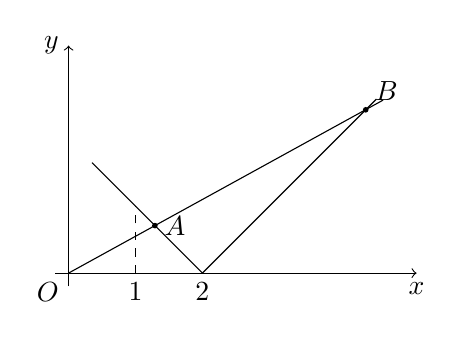
\begin{tikzpicture}[scale=0.85]
\draw[->] (-0.2,0) -- (5.2,0) node[below]{$x$};
\draw[->] (0,-0.2) -- (0,3.4) node[left]{$y$};
\node[below left] at (0,0) {$O$};
\draw (2,0) -- (0.35,1.65);
\draw (2,0) -- (4.6,2.6);
\draw (0,0) -- (4.7,2.585);
\draw[dashed] (1,0) -- (1,1);
\node[below] at (1,0) {$1$};
\node[below] at (2,0) {$2$};
\coordinate (A) at (1.29,0.71); \fill (A) circle (1.2pt); \node[right] at (A) {$A$};
\coordinate (B) at (4.44,2.44); \fill (B) circle (1.2pt); \node[above right] at (B) {$B$};
\end{tikzpicture}
\end{center}
\step{由 $0<k<1$，得 $x_A>1$，}
\step{所以关于 $x$ 的不等式 $k\lvert x\rvert-\lvert x-2\rvert>0$ 恰好有 $4$ 个整数解，是 $2,3,4,5$，}
\step{由 $\begin{cases}y=kx\\ y=x-2\end{cases}\Rightarrow x_B=\dfrac2{1-k}\in(5,6]$，故 $\dfrac35<k\leqslant\dfrac23$.}
\solend
\fi

\item 设集合 $S=\{1,2,3,\cdots,10\}$，$S$ 的子集 $A$ 满足 $A\cap\{1,2,3\}\neq\varnothing$，$A\cup\{4,5,6\}\neq S$，这样的子集 $A$ 的个数为\blankline[4.4em].

\ifanswer
\solbegin
\step{先求使 $A\cap\{1,2,3\}\neq\varnothing$ 成立的 $S$ 的子集 $A$ 的个数 $N_1$，}
\step{在 $\{1,2,3\}$ 中取出至少一个元素的方式有 $7$ 种，}
\step{而集合 $\{4,5,\cdots,10\}$ 的子集有 $2^7$ 个，因此 $N_1=7\times2^7=896$，}
% 注：下一行原卷印作“$A\cup\{4,5,6\}\neq S$”，按上下文应为“$=S$”，照录未改（见文件头“原卷笔误/存疑”①）。
\step{再扣除其中使 $A\cup\{4,5,6\}\neq S$ 的集合 $A$ 的个数 $N_2$，}
\step{这些取法中 $1$，$2$，$3$，$7$，$8$，$9$，$10$ 均被取出，}
\step{而集合 $\{4,5,6\}$ 的子集有 $2^3$ 个，因此 $N_2=2^3=8$，}
\step{从而满足条件的子集 $A$ 的个数为 $N_1-N_2=896-8=888$.}
\solend
\fi

\end{enumerate}

\bigsec{二、选择题}

\begin{enumerate}
\setcounter{enumi}{12}

\item 已知 $a>b$，下列不等式中一定成立是\mbox{（\quad）}

\keepwithprev
A. $a^2>b^2$\qquad B. $ac^2>bc^2$\qquad C. $\dfrac1a<\dfrac1b$\qquad D. $a+3>b-4$

\ifanswer
\solbegin
\step{对于 $A$，当 $a=-2$，$b=-4$ 时，不等式不成立，故 $A$ 错误；}
\step{对于 $B$，当 $c=0$ 时，不等式不成立，故 $B$ 错误；}
\step{对于 $C$，当 $a=2$，$b=-4$ 时，不等式不成立，故 $C$ 错误；}
\step{对于 $D$，因为 $a>b$，$3>-4$，必有 $a+3>b-4$ 成立，故 $D$ 正确.}
\solend
\fi

\item 已知集合 $M$ 满足 $\{2,3\}\subseteq M\subseteq\{1,2,3,4,5\}$，那么这样的集合 $M$ 的个数为\mbox{（\quad）}

\keepwithprev
A. $6$\qquad B. $7$\qquad C. $8$\qquad D. $9$

\ifanswer
\solbegin
\step{集合 $M$ 满足 $\{2,3\}\subseteq M\subseteq\{1,2,3,4,5\}$，所以 $2\in M$，$3\in M$，}
\step{故集合 $M$ 的个数为 $2^3=8$. 故选 $C$.}
\solend
\fi

\item 已知集合 $A=\{x\mid x=2k,k\in\Z\}$，$B=\{x\mid x=4m+6n,m,n\in\Z\}$，则\mbox{（\quad）}

\keepwithprev
A. $B\subset A$\qquad B. $A\subset B$\qquad C. $A=B$\qquad D. $B\neq A$

\ifanswer
\solbegin
\step{$B=\{x\mid x=4m+6n,m,n\in\Z\}$，$B$ 中的元素都是偶数，}
\step{所以 $B$ 的元素都是 $A$ 的元素，$B\subseteq A$；}
\step{$A=\{x\mid x=4(-k)+6k,k\in\Z\}$，则 $A$ 的元素都是 $B$ 的元素，$A\subseteq B$；}
\step{所以 $A=B$. 故选 $C$.}
\solend
\fi

\item 已知集合 $A=[1,a]\cup[a^3,a^4]$，集合 $B=\{x\mid x=x_1-x_2$，其中 $x_1,x_2\in A\}$. 若集合 $B$ 表示的区间为一个闭区间，则 $a$ 的取值范围为\mbox{（\quad）}

\keepwithprev
A. $a$ 取遍任意大于 $1$ 的实数\qquad B. $a\geqslant2$

C. $a\geqslant\dfrac{1+\sqrt5}2$\qquad D. $a\geqslant1+\sqrt2$

\ifanswer
\solbegin
\step{由题意得 $a^3>a>1$，则 $x_1-x_2$ 的最小值为 $1-a^4$，最大值为 $a^4-1$，}
\step{所以 $B=[1-a^4,a^4-1]$，}
\step{又因为 $a^4-a^3-(a-1)=a^3(a-1)-(a-1)=(a^3-1)(a-1)>0$，}
\step{所以 $a^4-a^3>a-1$，又集合 $B$ 表示的区间为一个闭区间，}
\step{则 $a^3-a\leqslant a^4-a^3$，化简得 $a^2-a-1\geqslant0$，又 $a>1$，解得 $a\geqslant\dfrac{1+\sqrt5}2$.}
\step{故选 $C$.}
\solend
\fi

\end{enumerate}

\bigsec{三、解答题}

\begin{enumerate}
\setcounter{enumi}{16}

\item 设全集 $U=\R$，集合 $A=\{x\mid\lvert x+3\rvert\leqslant4\}$，集合 $B=\{x\mid a-2\leqslant x\leqslant1+2a\}$，其中 $a\in\R$.

（1）若 $a=\dfrac12$，求 $A\cap B$；

（2）若 $A\cap B=\varnothing$，求 $a$ 的取值范围.

\ifanswer
\solbegin
\stepm{(1)}{由 $\lvert x+3\rvert\leqslant4$，得 $-4\leqslant x+3\leqslant4$，解得 $-7\leqslant x\leqslant1$，}
\step{所以 $A=\{x\mid-7\leqslant x\leqslant1\}$，}
\step{当 $a=\dfrac12$ 时，$a-2=\dfrac12-2=-\dfrac32$，$1+2a=1+2\times\dfrac12=2$，}
\step{$B=\left\{x\mid-\dfrac32\leqslant x\leqslant2\right\}$，$A\cap B=\left\{x\mid-\dfrac32\leqslant x\leqslant1\right\}$，即 $\left[-\dfrac32,1\right]$.}
\stepm{(2)}{若 $A\cap B=\varnothing$，分两种情况讨论，}
\step{①当 $B\neq\varnothing$ 时，$a-2\leqslant1+2a$，即 $a\geqslant-3$，}
\step{要满足 $A\cap B=\varnothing$，则 $1+2a<-7$ 或 $a-2>1$，}
\step{由 $1+2a<-7$，得 $a<-4$，与 $a\geqslant-3$ 无交集，无解，}
\step{由 $a-2>1$ 得 $a>3$，符合 $a\geqslant-3$，}
\step{②当 $B=\varnothing$ 时，有 $a-2>1+2a$，解得 $a<-3$，满足 $A\cap B=\varnothing$；}
\step{综上，$a$ 的取值范围是 $(-\infty,-3)\cup(3,+\infty)$.}
\solend
\fi

\ansspace

\item （1）已知 $a>b>0$，比较 $\dfrac{a+b}{a^2+b^2}$ 与 $\dfrac1{a-b}$ 的大小并说明理由；

（2）已知 $-2\leqslant x\leqslant-1$，$2\leqslant y\leqslant3$，求 $2x-y$ 的取值范围.

\ifanswer
\solbegin
\stepm{(1)}{$\dfrac{a+b}{a^2+b^2}-\dfrac1{a-b}=\dfrac{(a^2-b^2)-(a^2+b^2)}{(a^2+b^2)(a-b)}=\dfrac{-2b^2}{(a^2+b^2)(a-b)}$，}
\step{因为 $a>b>0$，所以 $a^2(a-b)-b^2(b-a)=(a^2+b^2)(a-b)>0$，}
\step{$\dfrac{-2b^2}{(a^2+b^2)(a-b)}<0$，即 $\dfrac{a+b}{a^2+b^2}-\dfrac1{a-b}<0$，所以 $\dfrac{a+b}{a^2+b^2}<\dfrac1{a-b}$；}
\stepm{(2)}{由 $-2\leqslant x\leqslant-1$，$2\leqslant y\leqslant3$，得 $-4\leqslant2x\leqslant-2$，$-3\leqslant-y\leqslant-2$，}
\step{得 $-7\leqslant2x-y\leqslant-4$，即 $2x-y$ 的取值范围为 $[-7,-4]$.}
\solend
\fi

\ansspace

\item 设 $x_1$、$x_2$ 是关于 $x$ 的方程 $x^2-2(m+2)x+m^2-1=0$ 的两个实数根.

（1）若 $\dfrac1{x_1}+\dfrac1{x_2}=-4$，求 $m$ 的值；

（2）若 $x_1$、$x_2$ 是两个不相等的正数，求实数 $m$ 的取值范围.

\ifanswer
\solbegin
\stepm{(1)}{因为 $x_1$、$x_2$ 是关于 $x$ 的方程的两个实数根，}
\step{所以 $\Delta=(-2(m+2))^2-4(m^2-1)=16m+20\geqslant0$，解得 $m\geqslant-\dfrac54$，}
\step{由韦达定理得 $x_1+x_2=2(m+2)$，$x_1x_2=m^2-1$，}
\step{所以 $\dfrac1{x_1}+\dfrac1{x_2}=\dfrac{x_2+x_1}{x_1x_2}=\dfrac{2(m+2)}{m^2-1}=-4$，即 $2m^2+m=0$，}
\step{解得 $m=0$ 或 $m=-\dfrac12$；}
\stepm{(2)}{由题意得 $\begin{cases}x_1+x_2>0\\ x_1x_2>0\\ \Delta>0\end{cases}$，即 $\begin{cases}2(m+2)>0\\ m^2-1>0\\ (-2(m+2))^2-4(m^2-1)>0\end{cases}$，}
\step{解得 $-\dfrac54<m<-1$ 或 $m>1$.}
\solend
\fi

\ansspace

\ifanswer\else\needvspace{10\baselineskip}\fi
\item 已知集合 $A=\{x\mid x\leqslant2\text{ 或 }x\geqslant a\}$.

（1）若 $B=\left\{x\mid(x-2)\left(x-\dfrac{12}{7-a}\right)<0\right\}$，$A\cap B=\varnothing$，$A\cup B=\R$，求实数 $a$ 的值；

（2）若 $a=3$ 且 $b<2$，$B=\{x\mid x^2-b(b+1)x+b^3<0\}$，$A\cap B\cap\Z$ 的子集个数为 $4$ 个，求实数 $b$ 的取值范围.

\ifanswer
\solbegin
\stepm{(1)}{当 $a\leqslant2$ 时，$A=\{x\mid x\leqslant2\text{ 或 }x\geqslant a\}=\R$，必有 $B=\varnothing$，}
\step{即不等式 $(x-2)\left(x-\dfrac{12}{7-a}\right)<0$ 无解，}
\step{必有 $\dfrac{12}{7-a}=2$，解得 $a=1$，符合题意，}
\step{当 $a>2$ 时，$A=(-\infty,2]\cup[a,+\infty)$，}
\step{若 $A\cap B=\varnothing$，$A\cup B=\R$，则 $B=(2,a)$，}
\step{即方程 $(x-2)\left(x-\dfrac{12}{7-a}\right)=0$ 的两个根是 $2$ 和 $a$，所以 $\dfrac{12}{7-a}=a$，}
\step{解得 $a=3$ 或 $a=4$，符合题意，}
\step{综上，实数 $a$ 的值为 $1$ 或 $3$ 或 $4$；}
\stepm{(2)}{由 $A\cap B\cap\Z$ 的子集个数为 $4$ 个，即 $A\cap B\cap\Z$ 中恰好有 $2$ 个整数元素，}
\step{由 $a=3$，则 $A=(-\infty,2]\cup[3,+\infty)$，}
\step{由 $x^2-b(b+1)x+b^3=(x-b^2)(x-b)<0$，又 $b<2$，}
\step{当 $1<b<2$ 时，$1<b^2<4$ 且 $b^2>b$，则 $B=(b,b^2)$，}
\step{则 $A\cap B=(b,2]\cup[3,b^2)$，}
\step{要使 $A\cap B\cap\Z$ 中恰好有 $2$ 个整数元素，即 $A\cap B\cap\Z=\{2,3\}$，}
\step{即 $\begin{cases}1<b<2\\ 3<b^2<4\end{cases}$，解得 $\sqrt3<b<2$，符合题意，}
\step{当 $b=1$ 或 $b=0$ 时，$B=\varnothing$，此时 $A\cap B\cap\Z=\varnothing$，不符合题意，舍去，}
\step{当 $0<b<1$ 时，$0<b^2<1$ 且 $b^2<b$，则 $B=(b^2,b)$，}
\step{此时 $A\cap B\cap\Z=\varnothing$，不符合题意，舍去，}
\step{当 $-1<b<0$ 时，$0<b^2<1$ 且 $b^2>b$，则 $B=(b,b^2)$，}
\step{此时 $A\cap B\cap\Z=\{0\}$，即 $A\cap B\cap\Z$ 中只有 $1$ 个元素，不符合题意，舍去，}
\step{当 $b\leqslant-1$ 时，$b^2\geqslant1$ 且 $b^2>b$，则 $B=(b,b^2)$，}
\step{此时 $A\cap B\cap\Z\supseteq\{-1,0,1\}$，即 $A\cap B\cap\Z$ 中至少有 $3$ 个元素，}
\step{不符合题意，舍去，}
\step{综上，实数 $b$ 的取值范围为 $(\sqrt3,2)$.}
\solend
\fi

\ansspace*[7]

\item 已知集合 $A=\{a_1,a_2,a_3,\cdots,a_n\}$ 中的元素均为正整数，其中 $n\in\N$ 且 $n\geqslant3$. 若对任意 $x,y\in A(x\neq y)$，都有 $\lvert x-y\rvert\geqslant\dfrac{xy}k$，则称集合 $A$ 具有性质 $M_k$.

（1）集合 $A=\{1,2,a\}$ 具有性质 $M_3$，求 $a$ 的最小值；

（2）若集合 $A$ 具有性质 $M_{24}$，且 $A$ 中最小元素和最大元素分别为 $a,b$，求证：$\dfrac1a-\dfrac1b\geqslant\dfrac{n-1}{24}$；

（3）已知集合 $A$ 具有性质 $M_{24}$，求 $A$ 中元素个数的最大值，并说明理由.

\ifanswer
\solbegin
\stepm{(1)}{由性质 $M_3$ 定义得 $\begin{cases}a-1\geqslant\dfrac a3\\ a-2\geqslant\dfrac{2a}3\end{cases}\Rightarrow\begin{cases}a\geqslant\dfrac32\\ a\geqslant6\end{cases}\Rightarrow a\geqslant6$，且 $a\subseteq\N^*$，}
% 注：上一行原卷印作“$a\subseteq\N^*$”，应为“$a\in\N^*$”，照录未改（见文件头“原卷笔误/存疑”②）。
\step{所以 $a$ 的最小值为 $6$.}
\stepm{(2)}{由题意得 $\lvert a_i-a_{i+1}\rvert\geqslant\dfrac{a_ia_{i+1}}{24}$，$(i=1,2,3,\cdots,n-1)$，且 $a_1<\cdots<a_n$，}
\step{所以 $a_{i+1}-a_i\geqslant\dfrac{a_ia_{i+1}}{24}\Rightarrow\dfrac1{a_i}-\dfrac1{a_{i+1}}\geqslant\dfrac1{24}$，$(i=1,2,3,\cdots,n-1)$，}
\step{所以 $\dfrac1{a_1}-\dfrac1{a_2}+\dfrac1{a_2}-\dfrac1{a_3}+\cdots+\dfrac1{a_{n-1}}-\dfrac1{a_n}=\dfrac1{a_1}-\dfrac1{a_n}\geqslant\dfrac{n-1}{24}$，得证.}
\stepm{(3)}{由 (2) 得 $\begin{cases}\dfrac1{a_1}\geqslant\dfrac{n-1}{24}\\ a_1\geqslant1\end{cases}\Rightarrow\dfrac{n-1}{24}<1\Rightarrow n<25$，}
\step{同 (2) 证明得 $\dfrac1{a_i}-\dfrac1{a_n}\geqslant\dfrac{n-i}{24}$ 且 $i=1,2,3,\cdots,n-1$，故 $\dfrac1{a_i}>\dfrac{n-i}{24}$，}
\step{又 $a_i\geqslant i$，所以 $\dfrac1i>\dfrac{n-i}{24}\Rightarrow i(n-i)<24$ 在 $i=1,2,3,\cdots,n-1$ 上恒成立，}
\step{当 $n\geqslant10$，取 $i=5$，则 $i(n-i)=5(n-5)>24$，故 $n<10$，}
\step{当 $n\leqslant9$，则 $i(n-i)\leqslant\dfrac{(i+n-i)^2}4=\dfrac{n^2}4<24\Rightarrow n<\sqrt{96}$，即 $n\leqslant9$.}
\step{综上，集合 $A$ 中元素个数的最大值为 $9$.}
\solend
\fi

\end{enumerate}

\end{document}
"
%
% 原始材料：微信公众号“魔都数学加油站”文章，连载“27学年高一79”；
% 原文标题“27学年高一79——2026-2027年上海市南汇中学高一上10月月考”；
% 原文链接：https://mp.weixin.qq.com/s/bFvc7GVgPTaDGg_6JSSfGg。
% 页面标注发布时间 2026-10-24 21:00（上海）。
% 正文为 9 张 PNG 页（`原图/高一79_南汇中学_10月月考/01..09.png`），
% 尺寸混排（第 1、2、4、5、7、8 页为 4762×6735，第 3、6、9 页为 2560×3620），均按页序读取。
%
% 篇幅与题号：原卷自第 3 题起编号。填空题 3—12（10 题）、选择题 13—16（4 题）、
% 解答题 17—21（5 题），共 19 题。
%
% 讲评版：第 4 题只印【答案】，本稿只给 \ans{}；其余 18 题印【解析】。
% 选择题答案在解析末句“故选 D／C／C／C”。
%
% 副标题：原卷未印副标题。本稿按内容标作“集合与常用逻辑用语、不等式”。
%
% 原卷笔误/存疑（均照录未改，正文对应处另有 % 注）：
%   ① 第 12 题解析作“再扣除其中使 $A\cup\{4,5,6\}\neq S$ 的集合 $A$ 的个数 $N_2$”，
%      按上下文应为“$A\cup\{4,5,6\}=S$”，否则“这些取法中 $1,2,3,7,8,9,10$ 均被取出”
%      与 $N_2=2^3=8$ 都无法解释；原卷印作 $\neq$，照录未改。
%   ② 第 21 题 (1) 解析末作“且 $a\subseteq\N^*$”，$a$ 是集合的元素，应为 $a\in\N^*$；
%      原卷印作 $\subseteq$，照录未改。
%
% 与原卷的排版差异：
%   ① 原卷每题下直接印【答案】/【解析】，本稿按全稿惯例将答案与解析置于答案版；
%   ② 原卷未印副标题，本稿补出；填空横线统一排 \blankline[4.4em]；
%   ③ 原卷数集记号排斜体 $R$、$Z$、$N$，本稿按全稿惯例改用 $\R$、$\Z$、$\N$；
%   ④ 第 17—21 题的子问用行内“（1）（2）（3）”段，解析中的子问标号用 \stepm；
%   ⑤ 解答题按惯例加 \ansspace；选择题括号排 \mbox{（\quad）}；
%   ⑥ 第 11 题解析有一幅函数图象（$y=k\lvert x\rvert$ 与 $y=\lvert x-2\rvert$），
%      按原图形状用 TikZ 重排（仅答案版出）。
%
% 行数核对：逐题数 \step/\stepm 条数，合计 107 条（Q3：2；Q5：2；Q6：1；Q7：4；Q8：4；
% Q9：4；Q10：5；Q11：4；Q12：7；Q13：4；Q14：2；Q15：4；Q16：6；Q17：11；Q18：5；
% Q19：7；Q20：24；Q21：11）。原卷解析的换行按语意合并，未逐行强拆；第 4 题只印
% 【答案】，提 \ans{}，不计入 \step 账。
%
\documentclass[a4paper,11pt]{article}
\usepackage{common}

\begin{document}

\examtitlest[3]{2026--2027 年南汇中学高一上 10 月月考}{集合与常用逻辑用语、不等式}

\bigsec{一、填空题}

\begin{enumerate}
\setcounter{enumi}{2}

\item 不等式 $\dfrac{1-x}{x}>0$ 的解集为\blankline[4.4em].

\ifanswer
\solbegin
\step{原不等式化为 $x(x-1)<0$，转化为 $\begin{cases}x>0\\ x-1<0\end{cases}$ 或 $\begin{cases}x<0\\ x-1>0\end{cases}$，}
\step{解得 $0<x<1$，则不等式的解集为 $\{x\mid0<x<1\}$.}
\solend
\fi

\item 用反证法证明命题：“若 $x^2<1$，则 $-1<x<1$”时，应假设\blankline[4.4em].

\ifanswer
\ans{$x\geqslant1$ 或 $x\leqslant-1$}
\fi

\item 设 $k$ 为实数，关于 $x$ 的不等式 $kx^2+x+2<0$ 的解集为 $A$，若 $2\notin A$，则 $k$ 的取值范围是\blankline[4.4em].

\ifanswer
\solbegin
\step{因为关于 $x$ 的不等式 $kx^2+x+2<0$ 的解集为 $A$，且 $2\notin A$，}
\step{所以 $x=2$ 时，$k\times2^2+2+2\geqslant0$，解得 $k\geqslant-1$，则 $k$ 的取值范围为 $[-1,+\infty)$.}
\solend
\fi

\item 已知集合 $M=\{y\mid y=x^2-2x,x\in\R\}$，$N=\{x\mid y=\sqrt{4-x^2}\}$，则 $M\cup N=$\blankline[4.4em].

\ifanswer
\solbegin
\step{$M=[-1,+\infty)$，$N=[-2,2]$，则 $M\cup N=[-2,+\infty)$.}
\solend
\fi

\item 设集合 $A=\{-3,2\}$，集合 $B=\{x\mid mx+1=0\}$，且 $A\cup B=A$，则 $m$ 的值组成的集合是\blankline[4.4em].

\ifanswer
\solbegin
\step{由 $A\cup B=A$，得 $B\subseteq A$，}
\step{当 $m=0$ 时，$B=\varnothing$，满足题意，}
\step{当 $m\neq0$ 时，$B=\left\{-\dfrac1m\right\}$，所以 $-\dfrac1m=2$ 或 $-\dfrac1m=-3$，所以 $m=-\dfrac12$ 或 $m=\dfrac13$，}
\step{综上所述，$m$ 的值组成的集合是 $\left\{0,-\dfrac12,\dfrac13\right\}$.}
\solend
\fi

\item 若不等式 $\lvert x\rvert<a$ 的一个充分不必要条件为 $\dfrac{2x-1}{x-2}<1$，则实数 $a$ 的取值范围是\blankline[4.4em].

\ifanswer
\solbegin
\step{不等式 $\lvert x\rvert<a$，得 $-a<x<a$，}
\step{不等式 $\dfrac{2x-1}{x-2}<1$，即 $\dfrac{2x-1-(x-2)}{x-2}=\dfrac{x+1}{x-2}<0$，解得 $-1<x<2$，}
\step{又不等式 $\lvert x\rvert<a$ 的一个充分不必要条件为 $\dfrac{2x-1}{x-2}<1$，}
\step{得 $\begin{cases}a\geqslant2\\ -a\leqslant-1\end{cases}$，且两等号不同时成立，解得 $a\geqslant2$.}
\solend
\fi

\item 若对任意 $x\in\R$ 都有 $(m-1)x^2-(m-1)x-1<0$，则实数 $m$ 的取值范围是\blankline[4.4em].

\ifanswer
\solbegin
\step{当 $m-1\neq0$，即 $m\neq1$ 时，则有 $\begin{cases}m-1<0\\ (m-1)^2-4(m-1)\times(-1)<0\end{cases}$，}
\step{解得 $-3<m<1$；}
\step{当 $m-1=0$ 时，即当 $m=1$ 时，此时不等式为 $-1<0$ 恒成立，符合题意；}
\step{综上所述，实数 $m$ 的取值范围是 $(-3,1]$.}
\solend
\fi

\item 关于 $x$ 的方程 $\dfrac{x}{x-1}=\dfrac{k-x}{x^2-x}$ 的解集中只含有一个元素，则 $k$ 的可能取值构成的集合为\blankline[4.4em].

\ifanswer
\solbegin
\step{方程两边同时乘以 $x(x-1)$ 得 $x^2=k-x$，即 $x^2+x-k=0$，}
\step{①当其中一个解为增根时，方程也只有一个解，}
\step{(i) 若增根为 $0$ 时，$k=0$；(ii) 若增根为 $1$ 时，$k=2$；}
\step{②当 $\Delta=1+4k=0$，即 $k=-\dfrac14$ 时，方程 $x^2+x-k=0$ 只有一个解；}
\step{即 $k$ 的可能取值构成的集合为 $\left\{-\dfrac14,0,2\right\}$.}
\solend
\fi

\item 若关于 $x$ 的不等式 $k\lvert x\rvert>\lvert x-2\rvert$ 恰好有 $4$ 个整数解，则实数 $k$ 的取值范围是\blankline[4.4em].

\ifanswer
\solbegin
\step{由题意得 $0<k<1$，函数 $y=k\lvert x\rvert$ 与 $y=\lvert x-2\rvert$ 的图象如图：}
\begin{center}
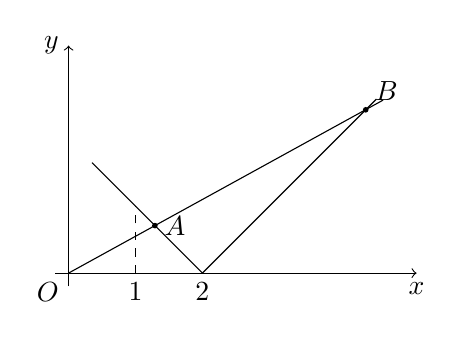
\begin{tikzpicture}[scale=0.85]
\draw[->] (-0.2,0) -- (5.2,0) node[below]{$x$};
\draw[->] (0,-0.2) -- (0,3.4) node[left]{$y$};
\node[below left] at (0,0) {$O$};
\draw (2,0) -- (0.35,1.65);
\draw (2,0) -- (4.6,2.6);
\draw (0,0) -- (4.7,2.585);
\draw[dashed] (1,0) -- (1,1);
\node[below] at (1,0) {$1$};
\node[below] at (2,0) {$2$};
\coordinate (A) at (1.29,0.71); \fill (A) circle (1.2pt); \node[right] at (A) {$A$};
\coordinate (B) at (4.44,2.44); \fill (B) circle (1.2pt); \node[above right] at (B) {$B$};
\end{tikzpicture}
\end{center}
\step{由 $0<k<1$，得 $x_A>1$，}
\step{所以关于 $x$ 的不等式 $k\lvert x\rvert-\lvert x-2\rvert>0$ 恰好有 $4$ 个整数解，是 $2,3,4,5$，}
\step{由 $\begin{cases}y=kx\\ y=x-2\end{cases}\Rightarrow x_B=\dfrac2{1-k}\in(5,6]$，故 $\dfrac35<k\leqslant\dfrac23$.}
\solend
\fi

\item 设集合 $S=\{1,2,3,\cdots,10\}$，$S$ 的子集 $A$ 满足 $A\cap\{1,2,3\}\neq\varnothing$，$A\cup\{4,5,6\}\neq S$，这样的子集 $A$ 的个数为\blankline[4.4em].

\ifanswer
\solbegin
\step{先求使 $A\cap\{1,2,3\}\neq\varnothing$ 成立的 $S$ 的子集 $A$ 的个数 $N_1$，}
\step{在 $\{1,2,3\}$ 中取出至少一个元素的方式有 $7$ 种，}
\step{而集合 $\{4,5,\cdots,10\}$ 的子集有 $2^7$ 个，因此 $N_1=7\times2^7=896$，}
% 注：下一行原卷印作“$A\cup\{4,5,6\}\neq S$”，按上下文应为“$=S$”，照录未改（见文件头“原卷笔误/存疑”①）。
\step{再扣除其中使 $A\cup\{4,5,6\}\neq S$ 的集合 $A$ 的个数 $N_2$，}
\step{这些取法中 $1$，$2$，$3$，$7$，$8$，$9$，$10$ 均被取出，}
\step{而集合 $\{4,5,6\}$ 的子集有 $2^3$ 个，因此 $N_2=2^3=8$，}
\step{从而满足条件的子集 $A$ 的个数为 $N_1-N_2=896-8=888$.}
\solend
\fi

\end{enumerate}

\bigsec{二、选择题}

\begin{enumerate}
\setcounter{enumi}{12}

\item 已知 $a>b$，下列不等式中一定成立是\mbox{（\quad）}

\keepwithprev
A. $a^2>b^2$\qquad B. $ac^2>bc^2$\qquad C. $\dfrac1a<\dfrac1b$\qquad D. $a+3>b-4$

\ifanswer
\solbegin
\step{对于 $A$，当 $a=-2$，$b=-4$ 时，不等式不成立，故 $A$ 错误；}
\step{对于 $B$，当 $c=0$ 时，不等式不成立，故 $B$ 错误；}
\step{对于 $C$，当 $a=2$，$b=-4$ 时，不等式不成立，故 $C$ 错误；}
\step{对于 $D$，因为 $a>b$，$3>-4$，必有 $a+3>b-4$ 成立，故 $D$ 正确.}
\solend
\fi

\item 已知集合 $M$ 满足 $\{2,3\}\subseteq M\subseteq\{1,2,3,4,5\}$，那么这样的集合 $M$ 的个数为\mbox{（\quad）}

\keepwithprev
A. $6$\qquad B. $7$\qquad C. $8$\qquad D. $9$

\ifanswer
\solbegin
\step{集合 $M$ 满足 $\{2,3\}\subseteq M\subseteq\{1,2,3,4,5\}$，所以 $2\in M$，$3\in M$，}
\step{故集合 $M$ 的个数为 $2^3=8$. 故选 $C$.}
\solend
\fi

\item 已知集合 $A=\{x\mid x=2k,k\in\Z\}$，$B=\{x\mid x=4m+6n,m,n\in\Z\}$，则\mbox{（\quad）}

\keepwithprev
A. $B\subset A$\qquad B. $A\subset B$\qquad C. $A=B$\qquad D. $B\neq A$

\ifanswer
\solbegin
\step{$B=\{x\mid x=4m+6n,m,n\in\Z\}$，$B$ 中的元素都是偶数，}
\step{所以 $B$ 的元素都是 $A$ 的元素，$B\subseteq A$；}
\step{$A=\{x\mid x=4(-k)+6k,k\in\Z\}$，则 $A$ 的元素都是 $B$ 的元素，$A\subseteq B$；}
\step{所以 $A=B$. 故选 $C$.}
\solend
\fi

\item 已知集合 $A=[1,a]\cup[a^3,a^4]$，集合 $B=\{x\mid x=x_1-x_2$，其中 $x_1,x_2\in A\}$. 若集合 $B$ 表示的区间为一个闭区间，则 $a$ 的取值范围为\mbox{（\quad）}

\keepwithprev
A. $a$ 取遍任意大于 $1$ 的实数\qquad B. $a\geqslant2$

C. $a\geqslant\dfrac{1+\sqrt5}2$\qquad D. $a\geqslant1+\sqrt2$

\ifanswer
\solbegin
\step{由题意得 $a^3>a>1$，则 $x_1-x_2$ 的最小值为 $1-a^4$，最大值为 $a^4-1$，}
\step{所以 $B=[1-a^4,a^4-1]$，}
\step{又因为 $a^4-a^3-(a-1)=a^3(a-1)-(a-1)=(a^3-1)(a-1)>0$，}
\step{所以 $a^4-a^3>a-1$，又集合 $B$ 表示的区间为一个闭区间，}
\step{则 $a^3-a\leqslant a^4-a^3$，化简得 $a^2-a-1\geqslant0$，又 $a>1$，解得 $a\geqslant\dfrac{1+\sqrt5}2$.}
\step{故选 $C$.}
\solend
\fi

\end{enumerate}

\bigsec{三、解答题}

\begin{enumerate}
\setcounter{enumi}{16}

\item 设全集 $U=\R$，集合 $A=\{x\mid\lvert x+3\rvert\leqslant4\}$，集合 $B=\{x\mid a-2\leqslant x\leqslant1+2a\}$，其中 $a\in\R$.

（1）若 $a=\dfrac12$，求 $A\cap B$；

（2）若 $A\cap B=\varnothing$，求 $a$ 的取值范围.

\ifanswer
\solbegin
\stepm{(1)}{由 $\lvert x+3\rvert\leqslant4$，得 $-4\leqslant x+3\leqslant4$，解得 $-7\leqslant x\leqslant1$，}
\step{所以 $A=\{x\mid-7\leqslant x\leqslant1\}$，}
\step{当 $a=\dfrac12$ 时，$a-2=\dfrac12-2=-\dfrac32$，$1+2a=1+2\times\dfrac12=2$，}
\step{$B=\left\{x\mid-\dfrac32\leqslant x\leqslant2\right\}$，$A\cap B=\left\{x\mid-\dfrac32\leqslant x\leqslant1\right\}$，即 $\left[-\dfrac32,1\right]$.}
\stepm{(2)}{若 $A\cap B=\varnothing$，分两种情况讨论，}
\step{①当 $B\neq\varnothing$ 时，$a-2\leqslant1+2a$，即 $a\geqslant-3$，}
\step{要满足 $A\cap B=\varnothing$，则 $1+2a<-7$ 或 $a-2>1$，}
\step{由 $1+2a<-7$，得 $a<-4$，与 $a\geqslant-3$ 无交集，无解，}
\step{由 $a-2>1$ 得 $a>3$，符合 $a\geqslant-3$，}
\step{②当 $B=\varnothing$ 时，有 $a-2>1+2a$，解得 $a<-3$，满足 $A\cap B=\varnothing$；}
\step{综上，$a$ 的取值范围是 $(-\infty,-3)\cup(3,+\infty)$.}
\solend
\fi

\ansspace

\item （1）已知 $a>b>0$，比较 $\dfrac{a+b}{a^2+b^2}$ 与 $\dfrac1{a-b}$ 的大小并说明理由；

（2）已知 $-2\leqslant x\leqslant-1$，$2\leqslant y\leqslant3$，求 $2x-y$ 的取值范围.

\ifanswer
\solbegin
\stepm{(1)}{$\dfrac{a+b}{a^2+b^2}-\dfrac1{a-b}=\dfrac{(a^2-b^2)-(a^2+b^2)}{(a^2+b^2)(a-b)}=\dfrac{-2b^2}{(a^2+b^2)(a-b)}$，}
\step{因为 $a>b>0$，所以 $a^2(a-b)-b^2(b-a)=(a^2+b^2)(a-b)>0$，}
\step{$\dfrac{-2b^2}{(a^2+b^2)(a-b)}<0$，即 $\dfrac{a+b}{a^2+b^2}-\dfrac1{a-b}<0$，所以 $\dfrac{a+b}{a^2+b^2}<\dfrac1{a-b}$；}
\stepm{(2)}{由 $-2\leqslant x\leqslant-1$，$2\leqslant y\leqslant3$，得 $-4\leqslant2x\leqslant-2$，$-3\leqslant-y\leqslant-2$，}
\step{得 $-7\leqslant2x-y\leqslant-4$，即 $2x-y$ 的取值范围为 $[-7,-4]$.}
\solend
\fi

\ansspace

\item 设 $x_1$、$x_2$ 是关于 $x$ 的方程 $x^2-2(m+2)x+m^2-1=0$ 的两个实数根.

（1）若 $\dfrac1{x_1}+\dfrac1{x_2}=-4$，求 $m$ 的值；

（2）若 $x_1$、$x_2$ 是两个不相等的正数，求实数 $m$ 的取值范围.

\ifanswer
\solbegin
\stepm{(1)}{因为 $x_1$、$x_2$ 是关于 $x$ 的方程的两个实数根，}
\step{所以 $\Delta=(-2(m+2))^2-4(m^2-1)=16m+20\geqslant0$，解得 $m\geqslant-\dfrac54$，}
\step{由韦达定理得 $x_1+x_2=2(m+2)$，$x_1x_2=m^2-1$，}
\step{所以 $\dfrac1{x_1}+\dfrac1{x_2}=\dfrac{x_2+x_1}{x_1x_2}=\dfrac{2(m+2)}{m^2-1}=-4$，即 $2m^2+m=0$，}
\step{解得 $m=0$ 或 $m=-\dfrac12$；}
\stepm{(2)}{由题意得 $\begin{cases}x_1+x_2>0\\ x_1x_2>0\\ \Delta>0\end{cases}$，即 $\begin{cases}2(m+2)>0\\ m^2-1>0\\ (-2(m+2))^2-4(m^2-1)>0\end{cases}$，}
\step{解得 $-\dfrac54<m<-1$ 或 $m>1$.}
\solend
\fi

\ansspace

\ifanswer\else\needvspace{10\baselineskip}\fi
\item 已知集合 $A=\{x\mid x\leqslant2\text{ 或 }x\geqslant a\}$.

（1）若 $B=\left\{x\mid(x-2)\left(x-\dfrac{12}{7-a}\right)<0\right\}$，$A\cap B=\varnothing$，$A\cup B=\R$，求实数 $a$ 的值；

（2）若 $a=3$ 且 $b<2$，$B=\{x\mid x^2-b(b+1)x+b^3<0\}$，$A\cap B\cap\Z$ 的子集个数为 $4$ 个，求实数 $b$ 的取值范围.

\ifanswer
\solbegin
\stepm{(1)}{当 $a\leqslant2$ 时，$A=\{x\mid x\leqslant2\text{ 或 }x\geqslant a\}=\R$，必有 $B=\varnothing$，}
\step{即不等式 $(x-2)\left(x-\dfrac{12}{7-a}\right)<0$ 无解，}
\step{必有 $\dfrac{12}{7-a}=2$，解得 $a=1$，符合题意，}
\step{当 $a>2$ 时，$A=(-\infty,2]\cup[a,+\infty)$，}
\step{若 $A\cap B=\varnothing$，$A\cup B=\R$，则 $B=(2,a)$，}
\step{即方程 $(x-2)\left(x-\dfrac{12}{7-a}\right)=0$ 的两个根是 $2$ 和 $a$，所以 $\dfrac{12}{7-a}=a$，}
\step{解得 $a=3$ 或 $a=4$，符合题意，}
\step{综上，实数 $a$ 的值为 $1$ 或 $3$ 或 $4$；}
\stepm{(2)}{由 $A\cap B\cap\Z$ 的子集个数为 $4$ 个，即 $A\cap B\cap\Z$ 中恰好有 $2$ 个整数元素，}
\step{由 $a=3$，则 $A=(-\infty,2]\cup[3,+\infty)$，}
\step{由 $x^2-b(b+1)x+b^3=(x-b^2)(x-b)<0$，又 $b<2$，}
\step{当 $1<b<2$ 时，$1<b^2<4$ 且 $b^2>b$，则 $B=(b,b^2)$，}
\step{则 $A\cap B=(b,2]\cup[3,b^2)$，}
\step{要使 $A\cap B\cap\Z$ 中恰好有 $2$ 个整数元素，即 $A\cap B\cap\Z=\{2,3\}$，}
\step{即 $\begin{cases}1<b<2\\ 3<b^2<4\end{cases}$，解得 $\sqrt3<b<2$，符合题意，}
\step{当 $b=1$ 或 $b=0$ 时，$B=\varnothing$，此时 $A\cap B\cap\Z=\varnothing$，不符合题意，舍去，}
\step{当 $0<b<1$ 时，$0<b^2<1$ 且 $b^2<b$，则 $B=(b^2,b)$，}
\step{此时 $A\cap B\cap\Z=\varnothing$，不符合题意，舍去，}
\step{当 $-1<b<0$ 时，$0<b^2<1$ 且 $b^2>b$，则 $B=(b,b^2)$，}
\step{此时 $A\cap B\cap\Z=\{0\}$，即 $A\cap B\cap\Z$ 中只有 $1$ 个元素，不符合题意，舍去，}
\step{当 $b\leqslant-1$ 时，$b^2\geqslant1$ 且 $b^2>b$，则 $B=(b,b^2)$，}
\step{此时 $A\cap B\cap\Z\supseteq\{-1,0,1\}$，即 $A\cap B\cap\Z$ 中至少有 $3$ 个元素，}
\step{不符合题意，舍去，}
\step{综上，实数 $b$ 的取值范围为 $(\sqrt3,2)$.}
\solend
\fi

\ansspace*[7]

\item 已知集合 $A=\{a_1,a_2,a_3,\cdots,a_n\}$ 中的元素均为正整数，其中 $n\in\N$ 且 $n\geqslant3$. 若对任意 $x,y\in A(x\neq y)$，都有 $\lvert x-y\rvert\geqslant\dfrac{xy}k$，则称集合 $A$ 具有性质 $M_k$.

（1）集合 $A=\{1,2,a\}$ 具有性质 $M_3$，求 $a$ 的最小值；

（2）若集合 $A$ 具有性质 $M_{24}$，且 $A$ 中最小元素和最大元素分别为 $a,b$，求证：$\dfrac1a-\dfrac1b\geqslant\dfrac{n-1}{24}$；

（3）已知集合 $A$ 具有性质 $M_{24}$，求 $A$ 中元素个数的最大值，并说明理由.

\ifanswer
\solbegin
\stepm{(1)}{由性质 $M_3$ 定义得 $\begin{cases}a-1\geqslant\dfrac a3\\ a-2\geqslant\dfrac{2a}3\end{cases}\Rightarrow\begin{cases}a\geqslant\dfrac32\\ a\geqslant6\end{cases}\Rightarrow a\geqslant6$，且 $a\subseteq\N^*$，}
% 注：上一行原卷印作“$a\subseteq\N^*$”，应为“$a\in\N^*$”，照录未改（见文件头“原卷笔误/存疑”②）。
\step{所以 $a$ 的最小值为 $6$.}
\stepm{(2)}{由题意得 $\lvert a_i-a_{i+1}\rvert\geqslant\dfrac{a_ia_{i+1}}{24}$，$(i=1,2,3,\cdots,n-1)$，且 $a_1<\cdots<a_n$，}
\step{所以 $a_{i+1}-a_i\geqslant\dfrac{a_ia_{i+1}}{24}\Rightarrow\dfrac1{a_i}-\dfrac1{a_{i+1}}\geqslant\dfrac1{24}$，$(i=1,2,3,\cdots,n-1)$，}
\step{所以 $\dfrac1{a_1}-\dfrac1{a_2}+\dfrac1{a_2}-\dfrac1{a_3}+\cdots+\dfrac1{a_{n-1}}-\dfrac1{a_n}=\dfrac1{a_1}-\dfrac1{a_n}\geqslant\dfrac{n-1}{24}$，得证.}
\stepm{(3)}{由 (2) 得 $\begin{cases}\dfrac1{a_1}\geqslant\dfrac{n-1}{24}\\ a_1\geqslant1\end{cases}\Rightarrow\dfrac{n-1}{24}<1\Rightarrow n<25$，}
\step{同 (2) 证明得 $\dfrac1{a_i}-\dfrac1{a_n}\geqslant\dfrac{n-i}{24}$ 且 $i=1,2,3,\cdots,n-1$，故 $\dfrac1{a_i}>\dfrac{n-i}{24}$，}
\step{又 $a_i\geqslant i$，所以 $\dfrac1i>\dfrac{n-i}{24}\Rightarrow i(n-i)<24$ 在 $i=1,2,3,\cdots,n-1$ 上恒成立，}
\step{当 $n\geqslant10$，取 $i=5$，则 $i(n-i)=5(n-5)>24$，故 $n<10$，}
\step{当 $n\leqslant9$，则 $i(n-i)\leqslant\dfrac{(i+n-i)^2}4=\dfrac{n^2}4<24\Rightarrow n<\sqrt{96}$，即 $n\leqslant9$.}
\step{综上，集合 $A$ 中元素个数的最大值为 $9$.}
\solend
\fi

\end{enumerate}

\end{document}
